% Use the University of Michigan thesis class
\documentclass[thesis]{thesis-umich}

\usepackage{amsmath,amssymb,amsthm,amsbsy}      % Math packages
\usepackage{environ}                            % Easy Environment defining
\usepackage{empheq}                             % Put boxes around long equations
\usepackage{mathtools}                          % ceil command
\usepackage{enumerate,enumitem}                 % Numbered list and formatting
\usepackage{graphicx}                           % Graphics
\usepackage{placeins}                           % Allows for \FloatBarrier command (constrains float placement)
\usepackage[bottom]{footmisc}                   % Footnotes to be bottom aligned
\usepackage[super]{nth}                         % 1st, 2nd, etc properly formatted automatically
\usepackage{multirow,multicol}                  % Multiple rows/columsn in tables
\usepackage{caption}                            % Allows for \caption*
\usepackage{subcaption}                         % Subfigures
\usepackage{siunitx}                            % Column type S in tables
% \usepackage[chapter]{algorithm}
% \usepackage{algcompatible}
% \usepackage{algpseudocode}
\usepackage{booktabs}                           % Better table formatting
\usepackage{microtype}                          % Better line breaking and formatting
\usepackage{breakcites}                         % Better line breaking with cites?
\usepackage[backend=bibtex,                     % Use bibtex backend
            natbib=true,                        % Use natbib
            refsection=chapter,                 % Break references by chapter
            sorting=none,
            style=numeric-comp,
            maxcitenames=2]{biblatex}       % Biblatex - Reference management. Citations in-order
\usepackage{etoolbox}                           % Command definitions
\usepackage{tikz}                               % TikZ figures
% \usepackage{titletoc}                           % Chapter TOC
\usepackage{xstring}                            % String processing stuff
\usepackage[nameinlink,capitalize]{cleveref}    % Clever references (\cref, \Cref)
\usepackage[final]{pdfpages}                    % \includepdf
\usepackage{blindtext}

% Extra stylings
% Prioritize DOI over URL
\renewbibmacro*{doi+eprint+url}{%
  \iftoggle{bbx:doi}
    {\printfield{doi}}
    {}%
  \newunit\newblock
  \iftoggle{bbx:eprint}
    {\usebibmacro{eprint}}
    {}%
  \newunit\newblock
  \iftoggle{bbx:url}
    {\iffieldundef{doi}{\usebibmacro{url}}}
    {}%
}

% Itemize separations
\setlist[itemize]{topsep=0pt,itemsep=-1ex,partopsep=1ex,parsep=1ex}

% Cref for subequations
\crefname{subeqs}{Eqs.}{Eqs.}
\Crefname{subeqs}{Eqs.}{Eqs.}
\crefformat{subeqs}{#2Eqs.~(#1)#3}
\Crefformat{subeqs}{#2Eqs.~(#1)#3}

% Center bibliography heading
\defbibheading{bibliography}[\bibname]{%
  \chapter*{\centering #1}%
  \markboth{#1}{#1}}

% Extra macros
%%%%%%%%%%%%%%%%%%%%%%%%%%%%%%%%%%%%
% Aligned equation
\NewEnviron{aequation}{%
    \begin{equation}\begin{split}
        \BODY
    \end{split}\end{equation}
}

% Xparse extension
\newcommand{\DeclareAutoPairedDelimiter}[3]{%
  \expandafter\DeclarePairedDelimiter\csname Auto\string#1\endcsname{#2}{#3}%
  \DeclareRobustCommand{#1}{\csname Auto\string#1\endcsname*}}
\ExplSyntaxOn
\DeclareExpandableDocumentCommand{\IfNoValueOrEmptyTF}{mmm}{
  \IfNoValueTF{#1}{#2}{\tl_if_empty:nTF {#1} {#2} {#3}}
}
\ExplSyntaxOff
%%% General Mathematics %%%
\newcommand{\defined}{\equiv}
\newcommand{\pluseq}{\mathrel{+}=}        % Accumulation (plus-equals)
\DeclareDocumentCommand{\avg}{ m }{\overline{#1}}
\DeclareDocumentCommand{\vec}{ m }{\boldsymbol{#1}}             % Bold vectors
\DeclareDocumentCommand{\lvec}{ m }{\underline{\vec{#1}}}       % underline bold vectors
\DeclareDocumentCommand{\uvec}{ m }{\vec{\widehat{#1}}}         % Unit-vector
\DeclareDocumentCommand{\mat}{ m }{\boldsymbol{#1}}
\newcommand{\vdot}{\boldsymbol{\cdot}}           % Bold dot-mulitply
\newcommand{\grad}{\vec{\nabla}}
\newcommand{\dif}{\mathop{}\!\mathrm{d}}  % d for integrals
\DeclareDocumentCommand{\deriv}{ m m }{                   % Derivatives
  \frac{\dif{#1}}{\dif{#2}}
}
\DeclareDocumentCommand{\pderiv}{ m m }{                  % Partial derivatives
  \frac{\partial{#1}}{\partial{#2}}
}
\DeclarePairedDelimiter{\abs}{\lvert}{\rvert}       % Absolute value
\DeclarePairedDelimiter{\ceil}{\lceil}{\rceil}      % Ceiling
\DeclarePairedDelimiter{\floor}{\lfloor}{\rfloor}   % Floor
\DeclareAutoPairedDelimiter{\lrabs}{\lvert}{\rvert}       % Absolute value
\DeclareAutoPairedDelimiter{\lrceil}{\lceil}{\rceil}      % Ceiling
\DeclareAutoPairedDelimiter{\lrfloor}{\lfloor}{\rfloor}   % Floor
%%% Mathematical Operators %%%
\DeclareDocumentCommand{\intl}{ o o }{    % Integral w/ or w/o limits
  \IfValueTF{#1}
  {
    \IfValueTF{#2}
    {\int_{#1}^{#2}}
    {\int_{#1}}
  }
  {\int}
}
\DeclareDocumentCommand{\suml}{ o o }{    % Sum w/ or w/o limits
  \IfValueTF{#1}
  {
    \IfValueTF{#2}
    {\mathchoice{\sum\limits_{#1}^{#2}}{\sum\limits_{#1}^{#2}}{\sum_{#1}^{#2}}{\sum_{#1}^{#2}}}
    {\mathchoice{\sum\limits_{#1}}{\sum\limits_{#1}}{\sum_{#1}}{\sum_{#1}}}
  }
  {\sum}
}
\DeclareDocumentCommand{\prodl}{ o o }{    % Product w/ or w/o limits
  \IfValueTF{#1}
  {
    \IfValueTF{#2}
    {\mathchoice{\prod\limits_{#1}^{#2}}{\prod\limits_{#1}^{#2}}{\prod_{#1}^{#2}}{\prod_{#1}^{#2}}}
    {\mathchoice{\prod\limits_{#1}}{\prod\limits_{#1}}{\prod_{#1}}{\prod_{#1}}}
  }
  {\prod}
}

%%% Neutronics Quantities %%%
% Dimensional Quantities %
\newcommand{\Direction}{\Omega}           % General Direction symbol
\newcommand{\Azimuthal}{\varphi}          % General Azimuthal Angle
\newcommand{\Polar}{\theta}               % General Polar Angle
\newcommand{\PolarCos}{\mu}               % General Polar cosine
\newcommand{\location}{x}                 % General Location symbol
\newcommand{\Bounds}{X}                   % General Location symbol (bounds)
\newcommand{\Time}{t}                     % General Time symbol
\newcommand{\dir}{\uvec{\Direction}}      % Direction vector
\newcommand{\loc}{\vec{\location}}        % Location vector
\newcommand{\Loc}{\vec{X}}                % Global location vector
\newcommand{\Eprime}{E^{\prime}}          % Integration energy
\newcommand{\dirprime}{\dir^{\prime}}     % Integration direction
\newcommand{\ddir}{\dif{\Direction}}
\newcommand{\ddirprime}{\dif{\Direction^{\prime}}}
\newcommand{\Weight}{w}

% Cross-sections
\newcommand{\CrossSection}{\Sigma}
\newcommand{\MicroCrossSection}{\sigma}
\newcommand{\OpticalThickness}{\tau}
\newcommand{\irchi}[2]{\raisebox{\depth}{$#1\chi$}} % inner command, used by \Spectrum
\DeclareRobustCommand{\Spectrum}{{\mathpalette\irchi\relax}}

% Flux
\newcommand{\AngularFlux}{\psi}
\newcommand{\ScalarFlux}{\phi}
\newcommand{\FluxMoment}{\Phi}
\newcommand{\Current}{\vec{J}}
\newcommand{\FluxSpectrum}{\Phi}

% Eigenvalues
\newcommand{\Eigenvalue}{\lambda}
\newcommand{\kEigenvalue}{k}
\newcommand{\keff}{\kEigenvalue_{\text{eff}}}

% Common terms
\newcommand{\fourpi}{4\pi}
\newcommand{\rfourpi}{\frac{1}{\fourpi}}

% Spherical harmonics
\DeclareDocumentCommand{\SH}{ O{\ell} O{n} O{\dir} }{\ensuremath{R^{#2}_{#1}(#3)}}
\DeclareDocumentCommand{\Region}{ O{i} }{\mathcal{R}_{#1}}
% Possessive textual citation
\NewDocumentCommand{\citetp}{s m}{%
    \IfBooleanTF{#1}%
        {\citeauthor{#2}'~\cite{#2}}%
        {\citeauthor{#2}'s~\cite{#2}}%
}

%%%%%%%%%%%%%%%%%%%%%%%%%%%%%%%%%%%%%%%%%%%%%%%%%%%%%%%%%%%%%%%%%%%%%%%%%%
\addbibresource{library}
\title{Parallel 3-D Method of Characteristics with Linear Source and Advanced Transverse Integration}
\author{Andrew Fitzgerald}
\department{Nuclear Engineering and Radiological Sciences}
\year=2020

\frontispiece{
  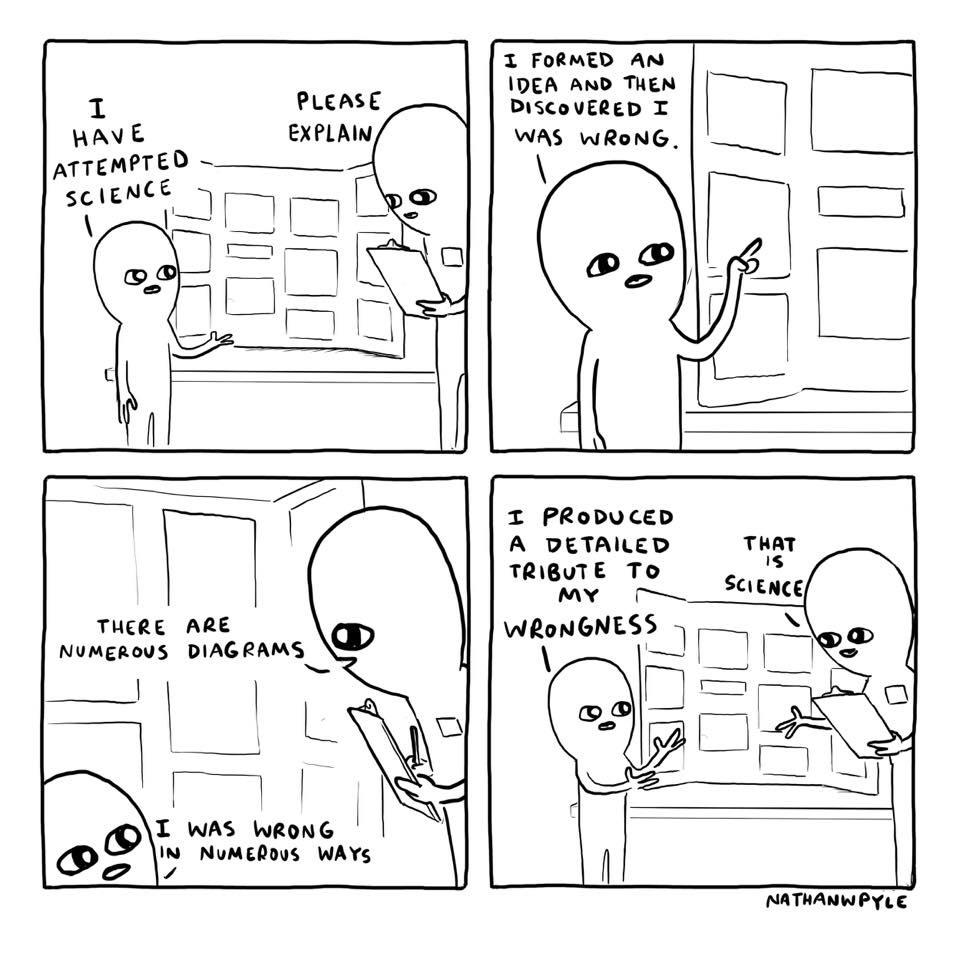
\includegraphics[width=0.75\linewidth]{Preface/front-comic.jpg}

  \hspace*{\fill} - Strange Planet, Nathan Pyle 2019
}
\frontpagestyle{1}

% Make it harder for widows and orphans to appear:
% \widowpenalty10000
% \clubpenalty10000

% Dedication
 \dedication{To my wife, Jinjuan, and our son, Charles.}%ZZZZ

% Acknowledgments
 \acknowledgments[6]{
  While this thesis represents my work over the past 5 years, this work would not exist without the contributions from many different people.

  I would like to thank the entirety of my thesis committee for guiding my research, and offering insights.
  In particular I would like to thank my chair, Professor Brendan Kochunas, whose thesis was the original inspiration for this work.
  I am thankful for his continued mentorship throughout my PhD studies, and his clear interest and dedication to helping this work progress.
  I am especially thankful to Professor Thomas Downar, my original advisor, who has been instrumental to the development of my studies.
  As an undergraduate, Professor Downar gave me the opportunity to work in his research group.
  Without this experience it is unlikely I would have pursued my PhD studies.
  I'd like to thank Professor Edward Larsen, whose passion for neutron transport has helped to keep me motivated throughout my studies.
  I owe a special thanks to Dr. Rodolfo Ferrer, whose work with the linear source served as a foundation to base parts of this work.

  The work of this thesis has relied heavily on the MPACT code;
    without the hard work of all the MPACT team developers, this work would certainly not have been possible for me.
  I am grateful for the opportunity to have worked on this code, alongside my colleagues, for the past 6 years.
  I would also like to express my gratitude to the \ac{DOE}, for funding the majority of my PhD studies,
    through the Nuclear Energy University Graduate fellowship.
    % CASL?

  Finally, I would like to thank my family, friends, and colleagues.
  My parents, who inspired my passion for mathematics and computer science.
  To my wife, Jinjuan, who has helped to keep me motivated throughout my studies.
  And my friends and colleagues who have allowed me to vent my countless struggles and frustrations over the course of my studies.
 }
%  This command sets the width of the acknowledgments area as a fraction
%  of the total width of the text area.
 \acknowledgmentswidth{0.95} %ZZZZ

% Committee
\committee{ %
    Assistant Professor Brendan Kochunas, Chair\\
    Professor Thomas Downar\\
    Dr. Rodolfo Ferrer\\
    Professor Emeritus Edward Larsen\\
    Professor Venkat Raman
}

% Commands to hide or show lists of figures, tables, etc.
% \hidelistoftables
% \hidelistoffigures %ZZZ check captions
\showlistoftables
\showlistoffigures %ZZZ check captions
\showlistofalgorithms
\hidelistofappendices

% Definition of any abbreviations used.
\abbreviations{
    \acro{MOC}[MoC]{Method of Characteristics}
    \acro{FS}{Flat Source}
    \acro{LS}{Linear Source}
    \acro{FSA}{flat-source approximation}
    \acro{LSA}{linear-source approximation}
    \acro{FSMOC}[FSMoC]{flat-source method of characteristics}
    \acro{LSMOC}[LSMoC]{linear-source method of characteristics}
    \acro{DOE}{Department of Energy}
    \acro{CASL}{Consortium for the Advanced Simulation of Light Water Reactors}
    \acro{LWR}{Light Water Reactor}
    \acro{PWR}{Pressurized Water Reactor}
    \acro{BWR}{Boiling Water Reactor}
    \acro{NEAMS}{Nuclear Energy Advanced Modeling and Simulation Program}
    \acro{PDE}{Partial Differential Equation}
    \acro{ODE}{Ordinary Differential Equation}
    \acro{PN}[$P_{N}$]{Spherical Harmonics}
    \acro{SPN}[S\ac{PN}]{Simplified \ac{PN}}
    \acro{CP}{Collision Probability}
    \acro{CDP}{method of Characteristic Direction Probabilities}
    \acro{SN}[$S_{N}$]{Discrete Ordinates}
    \acro{NDA}{non-linear diffusion acceleration}
    \acro{CMFD}{coarse mesh finite-difference}
    \acro{TH}[T/H]{thermal-hydraulic}
    \acro{TCP0}{transport-corrected $P_0$}
    \acro{DNPL}{direct neutron path linking}
    \acro{MRMB}{memory reduction technique for macroband}
    \acro{MRT}{modular ray-tracing}
    \acro{LEAF}{Legendre polynomial expansion of angular flux}
    \acro{VERA}{Virtual Environment for Reactor Analysis}
    \acro{VERA-CS}{Virtual Environment for Reactor Analysis Core Simulator}
    \acro{UO2}[UO$_2$]{UO$_2$}
    \acro{CPU}{central processing unit}
    \acro{GPU}{graphics processing unit}
    \acro{GPGPU}{general purpose graphics processing unit}
}

%%% This requires double spacing! go back and fix it in thesis.cls! %%%
\abstract{
  In the design and analysis of nuclear fission reactor systems, simulations are an essential tool for improving efficiency as well as safety.
  Neutronics simulations have always been limited by the available computational resources.
  This is because of the large discretizations that are needed for the neutron transport equation, which has a 6-dimensional phase space for steady-state eigenvalue problems.

  The ``gold standard'' for 3-D neutron transport simulations is Monte Carlo with explicit geometry representation because it treats all dependent variables continuously.
  However, there are significant remaining challenges for Monte Carlo methods that prohibit their widespread use, and put them at a disadvantage compared to deterministic methods.
  The ``gold standard'' for deterministic 3-D neutron transport is the 3-D \ac{MOC}.
  Numerous deterministic methods exist for solving the 3-D transport equation. Each of them has their own drawback.
  3-D \ac{MOC} is considered the ``best'' due to its ability to accurately model the exact geometry and approximate anisotropic scattering (other methods do just one of these well or become undesirably complex).
  The downside of the 3-D \ac{MOC} method is the substantial computational resources required to discretize the problem.

  Over the past decade, there has been renewed interest in assessing the state of the art for 3-D \ac{MOC} and the tractability of this problem on the newest computer architectures.
  Previous work made significant strides in parallelizing the \ac{MOC} algorithm for 100,000's of processors, but ultimately did not prove viable due to the extreme compute resources required.
  Since then there has been progress in making 3-D MOC less computationally burdensome by adopting more advanced discretization methods that lead to fewer spatial mesh regions and rays; namely the linear source approximation, and chord-classification or on-the-fly ray-tracing.
  The goal of this thesis is to continue progress in reducing the computational burden of \acf{MOC} calculations, with a particular focus on three-dimensional calculation.
  This thesis makes an effort to reach this goal through three related contributions: the utilization of graph-theory for spatial decomposition, improvements to the \ac{LSA} for multiphysics calculations, and a novel 3-D ray-tracing method with advanced transverse integration.

  Spatial decomposition is typically very beneficial, if not necessary, for whole-core direct transport methods.
  Previous works on 3-D \ac{MOC} calculations have used simple spatial decomposition schemes, that often resulted in poor load-balancing, particularly when using the \ac{LSA}.
  This work addresses this issue by utilizing graph partitioning methods to give a better load-balance, even in cases where the number of computational cells is very different in different regions of the reactor.

  The \ac{LSA} has previously been shown to allow for the use of a coarser mesh while maintaining accuracy in pure neutronics calculations.
  However, typically the problems of interest involve multiple physics such as isotopic depletion and \ac{TH} feedback.
  This work improves the \ac{LSA} method for such problems by re-formulating the equations to eliminate an inefficiency in cases with non-constant cross sections.
  This is shown to significantly improve run-times and reduce memory usage, even in such cases.

  Finally, a novel 3-D ray-tracing method, based on the macroband, is developed to reduce the number of characteristic tracks necessary for an accurate result.
  The method is compared against a traditional ray-tracing method for several benchmark problems.
  In several of these cases, the method is shown to significantly reduce the number of segments necessary for similar accuracy from a traditional ray-tracing method.
  The ray-tracing method is also shown to have very desirable properties such as near-monotonic convergence, and is able to act as more of a ``black-box'' solver.
}
\begin{document}
    \acresetall
    \chapter{Introduction}{\label{ch:Introduction}
    \section{Motivation}{\label{sec:Introduction:Motivation}
        Computer simulations have played an important role in the design and analysis of nuclear reactor systems over the past 60 years \cite{FewGroupDiffusion}.
        The methods used by these simulations have always been limited by the available computational resources; as such, in the 1950's two-group diffusion theory was used as a basis for simulation tools \cite{FewGroupDiffusion}.
        As computers became more powerful, multigroup diffusion calculations became the method of choice for \ac{LWR} design calculations.

        More accurate and detailed simulation tools allow for designs to have higher power density, and thus be more profitable, without compromising safety.
        However, computational resources have always limited the level of detail of simulation tools.
        Exponential increases in computing power, and high-performance computing clusters have made whole-core transport calculations possible \cite{CASMO-4,Apollo2-2010,DeCART,Denovo,Yang2010,Boyd2014,Collins2016,Gunow2018}.
        Programs such as \ac{CASL} and \ac{NEAMS} have focused on development of modern advanced simulation tools to address certain challenge problems.
        Large computing clusters are generally unavailable to reactor analysts in industry, and so using direct whole-core 3-D transport methods is not common outside academia or national laboratories.

        The ``gold standard'' of deterministic methods has been the 3-D \ac{MOC} \cite{Askew1972} due to its' ability to exactly model complicated geometries.
        At the time of writing, whole-core 3-D \ac{MOC} calculations are generally not possible without use of large computing clusters.
        This is due to the large discretizations that are necessary for the neutron transport equation, which has a 6-dimensional phase space for steady-state eigenvalue problems.
        In the past decade, there has been renewed interest in making 3-D \ac{MOC} more efficient and performant by using parallelism \cite{Kochunas2013}, modern \ac{GPU} architectures \cite{Boyd2014}, and ray-tracing storage techniques \cite{Sciannandrone2016, Gunow2016}.
        There has also been work done to make \ac{MOC} faster by improving the efficiency of the calculations by using higher-order approximations \cite{Ferrer2016,Gunow2018}.

        The bulk of this thesis work is comprised of three distinct, yet connected, topics, all with a focus on improving the feasibility of 3-D \ac{MOC} calculations.
        It is the author's opinion, that improving efficiency of 3-D \ac{MOC} calculations should be the primary focus of current research, as it is not feasible for industry to use thousands of processors.
        Thus, two techniques are utilized as part of this thesis work: the \acf{LSA}, and the macroray.

        The \ac{LSA} has been studied by other research groups \cite{Ferrer2016,Ferrer2018,Gunow2018}, and has been worked on as part of this thesis project; specifically, this work has led to improvements of the method for stability in near-void regions \cite{Fitzgerald2018}, and efficiency in multi-physics simulations \cite{Fitzgerald2019}.
        The \ac{LSA} is an approximation that is used to improve \ac{MOC} efficiency by reducing the number of computational cells required for accurate results.

        The macroray is a new ray-tracing technique under development as part of this thesis work; this technique is an extension of the two-dimensional macroband \cite{Villarino1992} ray-tracing technique.
        This technique has been shown to reduce the number of characteristic rays required for accurate results in two-dimensional flat-source calculations \cite{Yamamoto2005,Fevotte2007}.
        To the best of the author's knowledge, there have been no studies of this ray-tracing technique in three-dimensional ray-tracing calculations.
        Fewer characteristic rays results in more efficient calculations; the improvement in efficiency is expected to be more significant in 3-D calculations due to the square scaling of tracks with ray-spacing, rather than linear scaling in 2-D.
        Additionally, efficiency should be improved further by the \ac{LS} which allows for coarser cells and fewer track-segments.

        The third contribution of this thesis is work in improving parallel efficiency.
        While large scale parallelism on thousands of processors may not be feasible for industry, some degree of parallelism is necessary for whole-core calculations due to memory constraints.
        An automated spatial decomposition scheme based on graph theory, is developed leading to significantly improved parallel efficiency \cite{Fitzgerald2017,Fitzgerald2019a}.
    }
    \section{Outline}{\label{sec:Introduction:Outline}
        % The remainder of this document is structured as follows.
        % \Cref{ch:Neutron Transport Theory} gives an overview of neutron transport theory, with a focus on what is relevant to this work.
        % The derivation and details on the \acf{MOC} are provided in \cref{ch:The Method of Characteristics}, with a focus on the contributions made in this work.
        % Ray-tracing is an important aspect of \acf{MOC} calculations, and details about ray-tracing techniques are provided in \cref{ch:Ray-Tracing}.
    }

    % References
    \printbibliography
}
    \chapter{Neutron Transport Theory}{\label{ch:Neutron Transport Theory}
  %%% Continuous Energy quantities %%%
% Cross-sections
\DeclareDocumentCommand{\xst}{ O{\loc} O{E} }{\ensuremath{\CrossSection_{t}(#1,#2)}}
\DeclareDocumentCommand{\xsa}{ O{\loc} O{E} }{\ensuremath{\CrossSection_{a}(#1,#2)}}
\DeclareDocumentCommand{\xsf}{ O{\loc} O{\Eprime} }{\ensuremath{\CrossSection_{f}(#1,#2)}}
\DeclareDocumentCommand{\xss}{ o O{\loc} O{\dirprime\vdot\dir} O{\Eprime \to E}}{
    \IfNoValueOrEmptyTF{#1}
    {\ensuremath{\CrossSection_{s}(#2,#3,#4)}}
    {\ensuremath{\CrossSection_{s,#1}(#2,#4)}}
}
\DeclareDocumentCommand{\spect}{ O{\loc} O{E} }{\ensuremath{\Spectrum(#1,#2)}}
\DeclareDocumentCommand{\nufis}{ O{\loc} O{E^{\prime}} }{ \ensuremath{\nu\xsf[#1][#2] }}

% Flux
\DeclareDocumentCommand{\aflux}{ O{\loc} O{\dir} O{E} }{\ensuremath{\AngularFlux(#1,#2,#3)}}
\DeclareDocumentCommand{\sflux}{ O{\loc} O{E} }{\ensuremath{\ScalarFlux(#1,#2)}}
\DeclareDocumentCommand{\current}{ O{\loc} O{E} }{\ensuremath{\Current(#1,#2)}}
\DeclareDocumentCommand{\afluxmom}{ O{\loc} O{E} O{\ell} O{n} }{\FluxMoment^{#4}_{#3}(#1,#2)}

% Source
\DeclareDocumentCommand{\source}{ O{\loc} O{\dir} O{E} }{\ensuremath{Q(#1,#2,#3)}}
   % Continuous space, direction, and energy quantities
  \def\figpath{chapters/TransportTheory/figures/}
  \graphicspath{ {\figpath} }

  In this chapter, the basic theory behind the neutron transport equation, and the numerical methods used to solve it, are introduced.

  \section{Neutron Transport Equation}{\label{sec:NTT:Neutron Transport Equation}
    The mean behavior of neutrons in a (steady-state) system is described by the Boltzmann transport equation:
    \begin{subequations}\label[subeqs]{eqs:NTT:Boltzmann Transport}
      \begin{aequation}\label{eq:NTT:Boltzmann Transport}
        &\Big[\dir\vdot\grad + \xst[\loc][E]\Big]\aflux[\loc][\dir][E]
          = \\&\qquad\qquad
          \rfourpi\Bigg[
            \source[\loc][\dir][E]\\&\qquad\qquad
            + \intl[0][\infty]\intl[\fourpi]\xss[][\loc][\dirprime\vdot\dir][\Eprime\to E]\aflux[\loc][\dirprime][\Eprime]\ddirprime\dif{\Eprime}\\&\qquad\qquad
            + \spect\intl[0][\infty]\nufis[\loc][\Eprime]\intl[\fourpi]\aflux[\loc][\dirprime][\Eprime]\ddirprime\dif{\Eprime}
        \Bigg],
      \end{aequation}
      \begin{equation*}
        \forall\loc\in V, \quad \forall\dir\in\fourpi,\quad \forall E\in[0,\infty),
      \end{equation*}
      \begin{equation}\label{eq:NTT:Boundary Conditions}
        \aflux[\loc][\dir][E] = \psi^{b}(\loc,\dir,E),
      \end{equation}
      \begin{equation*}
        \forall\loc\in \delta V, \quad \forall\dir\vdot\vec{\hat{n}}<0, \quad, \forall E \in [0,\infty),
      \end{equation*}
    \end{subequations}
    where $\loc$ is the position vector, $\dir$ is the direction vector, $E$ is the neutron energy, $\CrossSection$ quantities are the macroscopic cross sections, $\AngularFlux$ is the angular flux, $\nu$ is the average number of neutrons produced per fission, $\Spectrum$ is the fission neutron energy spectrum, $\delta V$ is the problem boundary, and $\vec{\hat{n}}$ is the outward surface normal vector.

    The position vector, $\loc$, is a column vector of the spatial coordinates:
    \begin{equation}\label{eq:NTT:Location Vector}
      \loc \defined \begin{bmatrix}x\\y\\z\end{bmatrix}.
    \end{equation}
    The direction vector, $\dir$, is a column unit-vector that gives the direction of flight for neutrons, and is defined by
    \begin{subequations}\label[subeqs]{eqs:NTT:Direction Definitions}
      \begin{equation}\label{eq:NTT:Direction Vector}
        \dir \defined
          \begin{bmatrix}
            \Direction_x\\\Direction_y\\\Direction_z
          \end{bmatrix}
          =
          \begin{bmatrix}
            \sqrt{1-\PolarCos^2}\cos(\Azimuthal)\\
            \sqrt{1-\PolarCos^2}\sin(\Azimuthal)\\
            \PolarCos
          \end{bmatrix},
      \end{equation}
      where $\Azimuthal$ is the azimuthal angle, and $\PolarCos$ is the cosine of the polar angle $\Polar$,
      \begin{equation}\label{eq:NTT:Polar Cosine}
        \PolarCos \defined \cos(\Polar).
      \end{equation}
    \end{subequations}
    The spatial and angular coordinates systems are depicted visually in \cref{fig:NTT:Transport Coordinate System}.

    \begin{figure}[h]
      \centering
      \def\svgwidth{0.4\linewidth}
      \input{\figpath/TransportCoordinateSystem.pdf_tex}
      \caption{Depiction of the spatial and directional coordinate system used in the neutron transport equation.}
      \label{fig:NTT:Transport Coordinate System}
    \end{figure}

    The transport equation, given by \cref{eq:NTT:Boltzmann Transport}, is an equation that represents the balance of neutrons.
    The streaming term, $\dir\vdot\grad\aflux$, gives the rate at which neutrons are moving in or out of the of an infinitesimal volume in phase-space due to motion.
    The collision term, $\xst[\loc][E]\aflux$, gives the rate at which neutrons have interactions (collisions) with a nucleus of the surrounding material.
    The source terms make up the right-hand side of the equation, and are separated into three components: an external source, the scattering source, and the fission source.
    The scattering source, $\intl[0][\infty]\intl[\fourpi]\xss[][\loc][\dirprime\vdot\dir][\Eprime\to E]\aflux[\loc][\dirprime][\Eprime]\ddirprime\dif{\Eprime}$, gives the rate at which neutrons are scattered into the given direction and energy at a set point in space.
    The fission source, $\spect\intl[0][\infty]\nufis[\loc][\Eprime]\intl[\fourpi]\aflux[\loc][\dirprime][\Eprime]\ddirprime\dif{\Eprime}$, gives the production rate of neutrons due to fission events.
    The vast majority of fission events are prompt, though a small fraction of fission events emit \emph{delayed} neutrons.
    Generally, in steady-state calculations the difference between prompt and delayed fission neutrons is ignored.
    However, for transient calculations, capturing this difference is essential.
    The external source, $\source[\loc][\dir][E]$, is a generic term that accounts for neutrons produced by all other processes that are not dependent on the angular flux.

    Generally, reactor physicists are interested in reaction rates, that are useful for determining power production, rather than the angular flux.
    A reaction rate at a specific point, direction, and energy can be computed as the product of the reaction cross section and the angular flux,
    \begin{equation}\label{eq:NTT:Reaction Rate}
      R_r(\loc,\dir,E) = \Sigma_r(\loc,E)\aflux[\loc][\dir][E].
    \end{equation}
    Integration over a volume, energy range, and direction gives a total reaction rate.
    These quantities are the primary figures of merit for engineering applications.
    For convenience, it is useful to define derived quantities that are used in these calculations.
    The \emph{scalar flux}
    \begin{equation}\label{eq:NTT:Scalar Flux Definition}
      \sflux \defined \intl[\fourpi]\aflux\ddir,
    \end{equation}
    is the zeroth order angular moment.
    The neutron \emph{current} is a vector quantity, and is the first order angular moment of the angular flux
    \begin{equation}\label{eq:NTT:Current Definition}
      \current \defined \intl[\fourpi]\dir\aflux\ddir.
    \end{equation}
    Generally, the angular moments of the angular flux are defined as
    \begin{equation}\label{eq:NTT:Angular Flux Moments}
      \afluxmom \defined \intl[\fourpi]\SH\aflux\ddir,
    \end{equation}
    where $\SH$ are the real spherical harmonics functions defined by
    \begin{subequations}\label[subeqs]{eqs:NTT:Spherical Harmonics Definitions}
      \begin{equation}\label{eq:NTT:Real SH Functions}
        \SH \defined \sqrt{(2-\delta_{n,0})\frac{(\ell-\abs{n})!}{(\ell+\abs{n})!}} P_{\ell}^{\abs{n}}(\PolarCos) \mathcal{T}(\Azimuthal),
      \end{equation}
      where $P_{\ell}^{\abs{n}}(\PolarCos)$ is the Ferrer definition \cite{Trlifaj1958} of the associated Legendre Polynomial defined as
      \begin{equation}\label{eq:NTT:Associated Legendre Polynomial}
        P_{\ell}^{\abs{n}}(\PolarCos) \defined \left(1-\PolarCos^2\right)^{n/2} \frac{\dif^{n}}{\dif{\PolarCos}^n}P_{\ell}(\PolarCos), \quad n\geq0,
      \end{equation}
      and
      \begin{equation}\label{eq:NTT:SH Azimuthal Dependence}
        \mathcal{T}(\Azimuthal) \defined
          \begin{cases}
            \cos(n\Azimuthal), \quad \text{if}~n\geq0,\\
            \sin(\abs{n}\Azimuthal), \quad \text{otherwise}.
          \end{cases}
      \end{equation}
    \end{subequations}
  }

  \section{\texorpdfstring{$k$}{k}-Eigenvalue Problems}{\label{sec:NTT:k-Eigenvalue Problems}
    One of the most common calculations in reactor analysis is the simulation of reactor systems at operating conditions.
    A reactor operating at normal conditions is effectively unchanging in time.
    The common technique for solving this class of problems is to transform \cref{eq:NTT:Boltzmann Transport} into an eigenvalue problem, such that the fission source is scaled to preserve neutron balance:
    \begin{subequations}\label[subeqs]{eqs:NTT:Eigenvalue Transport Problem}
      \begin{aequation}\label{eq:NTT:Eigenvalue Transport Problem}
        \Big[\dir\vdot\grad &+ \xst\Big]\aflux
          =
          \rfourpi\Bigg[
            \source\\
            &+ \intl[0][\infty]\intl[\fourpi]\xss\aflux[\loc][\dirprime][\Eprime]\ddirprime\dif{\Eprime}\\\qquad\qquad
            &+ \frac{\spect}{\keff}\intl[0][\infty]\nufis\sflux[\loc][\Eprime]\dif{\Eprime}
          \Bigg],
      \end{aequation}
      \begin{equation*}
        \forall\loc\in V, \quad \forall\dir\in\fourpi,\quad \forall E\in[0,\infty),
      \end{equation*}
      \begin{equation}\label{eq:NTT:Eigenvalue:Boundary Conditions}
        \aflux[\loc][\dir][E] = \psi^{b}(\loc,\dir,E),
      \end{equation}
      \begin{equation*}
        \forall\loc\in \delta V, \quad \forall\dir\vdot\vec{\hat{n}}<0, \quad, \forall E \in [0,\infty),
      \end{equation*}
    \end{subequations}
    where $\keff$ is the inverse of the largest eigenvalue of the system $\Eigenvalue_1$.
    The multiplication factor, $\keff$, indicates the criticality of the system.
    If $\keff$ is one, then the system is \emph{critical} and will remain at the current conditions unless otherwise changed.
    A $\keff$ less than one means that the system is \emph{subcritical} and indicates the reactor system is unable to sustain the chain reaction of nuclear fission reactions to produce power.
    Finally, a $\keff$ greater than one indicates that a system is \emph{supercritical} and, if not changed, the neutron population will increase.

    Generally, this class of problems are solved iteratively.
    This will be discussed in more detail in \cref{sec:NTT:Source Iteration}, which lists algorithms for this iteration process.
    Still, \cref{eq:NTT:Eigenvalue Transport Problem} has a six-dimensional phase space and cannot, in general systems, be solved exactly.
    Numerical techniques must be used to obtain approximate solutions to this equation in calculations for realistic reactor systems.
    In the \cref{sec:NTT:Computational Methods}, an overview of several methods for solving this equation, or approximate forms of this equation, is provided.
  }

  \section{Computational Transport Methods}{\label{sec:NTT:Computational Methods}
    Generally, transport methods are divided into two broad categories: stochastic and deterministic.
    Stochastic methods, also called ``Monte Carlo'' methods, rely on random sampling to emulate the ``life'' of individual neutrons.
    Deterministic methods rely on discretization of the transport equation.
    The process of discretization introduces approximations.
    An overview of these different approaches is given in the following subsections.

    \subsection{Monte Carlo}{\label{ssec:NTT:Monte Carlo}
      Stochastic, or ``Monte Carlo'' methods are methods that simulate individual neutrons in the system.
      The simulation of each neutron relies on the random sampling of probability distributions for all aspects such as, where the \emph{free} neutron is born, the direction it is traveling in, the energy of the neutron, the distance to the next collision, and the type of collision event.
      This process is repeated until the neutron leaks out of the system or is absorbed, possibly inducing a fission event with other neutrons to simulate, for many different neutrons.

      Monte Carlo methods give a probabilistic estimate of the true solution as well as an associated uncertainty in that result.
      This class of methods is generally considered to be the most accurate because it is capable of representing the phase-space continuously.
      As more particles are simulated, the uncertainty in the estimated solution is reduced.

      For whole-core reactor analysis, the quantities of interest would typically require an extremely large number of individual neutron histories to be simulated, typically trillions.
      Variance reduction techniques are an area of active research that allow for quantities of interest to be estimated accurately with fewer histories. % [CITATION].
      However, Monte Carlo methods generally remain too expensive for whole-core calculations, and have challenges with multiphysics and time-dependent problems.
    }

    \subsection{Deterministic Methods}{\label{ssec:NTT:Deterministic Methods}
      In deterministic methods, it is generally not possible to represent the phase-space continuously.
      Thus these methods rely on discretization of the transport equation.
      In particular, spatial, directional, and energy discretization are common in these methods.
      %%% Multi-group Energy quantities %%%
\DeclareDocumentCommand{\gprime}{}{g^{\prime}}
% Cross-sections
\DeclareDocumentCommand{\xs}{ O{t} O{\loc} O{g}}{\ensuremath{\CrossSection_{#1}^{#3}(#2)}}
\DeclareDocumentCommand{\xst}{ O{\loc} O{g} }{\xs[t][#1][#2]}
\DeclareDocumentCommand{\xsa}{ O{\loc} O{g} }{\xs[a][#1][#2]}
\DeclareDocumentCommand{\xsf}{ O{\loc} O{\gprime} }{\xs[f][#1][#2]}
\DeclareDocumentCommand{\xss}{ o O{\loc} O{\dirprime\vdot\dir} O{\gprime \to g} }{
    \IfNoValueOrEmptyTF{#1}
    {\xs[s][#2,#3][#4]}
    {\xs[s,#1][#2][#4]}
}
\DeclareDocumentCommand{\spect}{ O{\loc} O{g} }{\ensuremath{\Spectrum^{#2}(#1)}}
\DeclareDocumentCommand{\nufis}{ O{\loc} O{\gprime} }{ \ensuremath{\nu\xsf[#1][#2]}}
\DeclareDocumentCommand{\D}{ O{\loc} O{g} }{\ensuremath{D^{#2}(#1)}}

% Flux
\DeclareDocumentCommand{\aflux}{ O{\loc} O{\dir} O{g} }{\ensuremath{\AngularFlux^{#3}(#1,#2)}}
\DeclareDocumentCommand{\sflux}{ O{\loc} O{\gprime} }{\ensuremath{\ScalarFlux^{#2}(#1)}}
\DeclareDocumentCommand{\current}{ O{\loc} O{g} }{\ensuremath{\Current^{#2}(#1)}}
\DeclareDocumentCommand{\fluxmoma}{ O{\ell} O{n} O{\loc} O{g} }{\ensuremath{\ScalarFlux^{#2,#4}_{#1}(#3)}}

% Source
\DeclareDocumentCommand{\source}{ O{\loc} O{\dir} O{g} }{\ensuremath{q^{#3}(#1,#2)}}
\DeclareDocumentCommand{\sourcemoma}{ O{\ell} O{n} O{\loc} O{g} }{\ensuremath{q^{#2,#4}_{#1}(#3)}}

      \subsubsection{The Multigroup Approximation}{\label{sssec:NTT:The Multigroup Approximation}
        The multigroup approximation is common in nearly every deterministic neutron transport method.
        This approximation discretizes the energy variable into discrete energy groups.
        Generally, cross sections have strong dependence on the energy of incident neutrons; this dependence is typically not smooth, due to the presence of resonances.
        Around resonance energies, the cross sections increase significantly, as observed in \cref{fig:NTT:Cross Section plot}.
        The data of this plot was provided by the ENDF/B-VIII.0 nuclear reaction data library \cite{ENDF8}.

        \begin{figure}[h]
          \centering
          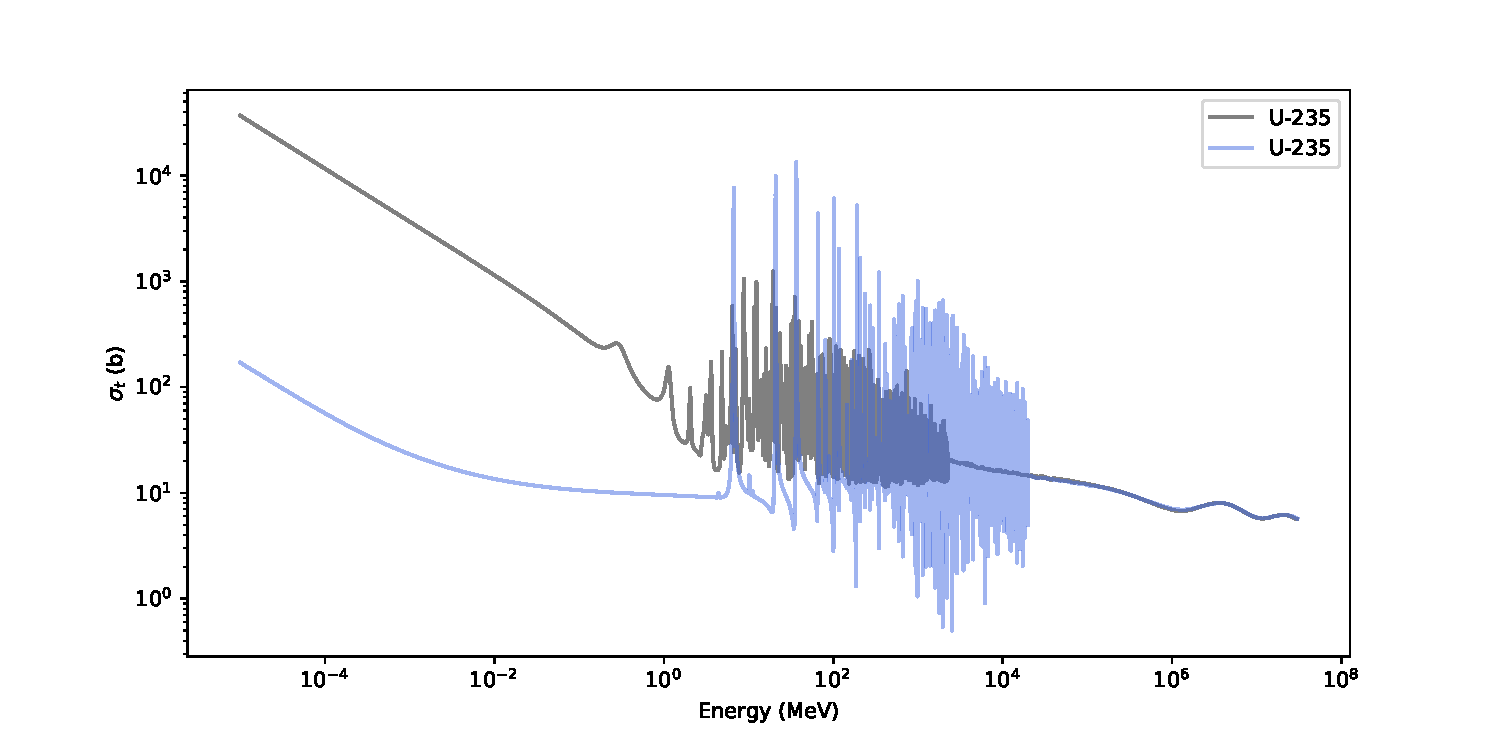
\includegraphics[width=0.85\linewidth]{\figpath/U235-8-XST}
          \caption{Uranium 235 and 238 total microscopic cross sections as a function of energy. Data provided through the ENDF/B-VIII.0 nuclear reaction data library.}
          \label{fig:NTT:Cross Section plot}
        \end{figure}

        The complicated dependence on energy would require hundreds of thousands of energy points to faithfully represent all the resonances of interest in thermal reactors.
        Modeling of this many energy points in whole-core simulations would be computationally impractical.
        The multigroup eigenvalue transport equation can be found by integrating the \cref{eq:NTT:Eigenvalue Transport Problem} over an energy energy interval $[E_{g}, E_{g-1})$, where $E_{g} > E_{g-1}$.
        \begin{aequation}\label{eq:NTT:MGEV Transport Problem w/ Anisotropic XS}
          \left[\dir\vdot\grad + \xst[\loc,\dir]\right]\aflux
            = \rfourpi\Bigg[&\suml[\gprime=1][G]\intl[\fourpi]\xss[][\loc][\dir,\dirprime]\aflux[\loc][\dirprime][\gprime]\ddirprime \\
            + &\frac{\spect}{\keff}\suml[\gprime=1][G]\nufis[\loc,\dir]\sflux[\loc]\Bigg],
        \end{aequation}
        \begin{equation*}
          \forall\loc, \quad \forall\dir\in\fourpi,\quad \forall g\in\{1,2,\ldots,G\},
        \end{equation*}
        where the multigroup quantities are defined by
        \begin{subequations}\label[subeqs]{eqs:NTT:Multigroup Quantities Anisotropic}
          \begin{equation}\label{eq:NTT:Multigroup Angular Flux}
            \aflux \defined \intl[E_g][E_{g-1}]\AngularFlux(\loc,\dir,E)\dif{E},
          \end{equation}
          \begin{equation}\label{eq:NTT:Multigroup Spectrum}
            \spect \defined \intl[E_g][E_{g-1}]\Spectrum(\loc,E)\dif{E},
          \end{equation}
          \begin{equation}\label{eq:NTT:Multigroup Total Cross Section Anisotropic}
            \xst[\loc,\dir] \defined \frac{\intl[E_{g}][E_{g-1}]\CrossSection_{t}(\loc,E)\AngularFlux(\loc,\dir,E)\dif{E}}{\aflux},
          \end{equation}
          \begin{equation}\label{eq:NTT:Multigroup Fission Cross Section Anisotropic}
            \nufis[\loc,\dir][g] \defined \frac{\intl[E_{g}][E_{g-1}]\nu\CrossSection_{f}(\loc,E)\AngularFlux(\loc,\dir,E)\dif{E}}{\aflux},
          \end{equation}
          \begin{equation}\label{eq:NTT:Multigroup Scattering Cross Section Anisotropic}
            \xss[][\loc][\dir,\dirprime] \defined \frac{\intl[E_{g}][E_{g-1}]\intl[E_{\gprime}][E_{\gprime-1}]\CrossSection_{s}(\loc,\dirprime\vdot\dir,\Eprime\to E)\AngularFlux(\loc,\dirprime,\Eprime)\dif{\Eprime}\dif{E}}{\aflux[\loc][\dirprime][\gprime]}.
          \end{equation}
        \end{subequations}

        By defining the cross sections in this way, no approximations have been made, and the reaction rates of each energy group are preserved.
        However, this approach has two issues: the cross sections are dependent on the angular flux which is not known \textit{a priori}, and have dependence on the neutron direction of flight.
        Generally, the dependence on the angular flux is addressed by solving a \emph{spatially} simplified problem to generate a continuous or fine-group neutron energy spectrum.
        This spectrum is then used as the weighting function (in place of $\aflux$) to ``collapse'' the cross sections into coarser multigroup values \cite{Knott2010}.
        This introduces an approximation into the transport equation.

        To eliminate the directional dependence of the multigroup cross sections, an additional approximation is made: isotropic angular flux spectrum,
        \begin{equation}\label{eq:NTT:Multigroup Isotropic Spectrum}
          \AngularFlux(\loc,\dir,E) \approx \rfourpi\FluxSpectrum(\loc, E).
        \end{equation}
        Using this approximate angular flux as the weighting function for multigroup cross sections in \cref{eq:NTT:MGEV Transport Problem w/ Anisotropic XS,eqs:NTT:Multigroup Quantities Anisotropic} can be simplified to
        \begin{aequation}\label{eq:NTT:MGEV Transport Problem}
          \left[\dir\vdot\grad + \xst\right]\aflux = \rfourpi\Bigg[&\suml[\gprime=1][G]\intl[\fourpi]\xss\aflux[\loc][\dirprime][\gprime]\ddirprime\\
              + \frac{\spect}{\keff}&\suml[\gprime=1][G]\nufis\intl[\fourpi]\aflux[\loc][\dirprime][\gprime]\ddirprime\Bigg],
        \end{aequation}
        \begin{equation*}
          \forall\loc, \quad \forall\dir\in\fourpi,\quad \forall g\in\{1,2,\ldots,G\},
        \end{equation*}
        where the approximated multigroup cross sections are defined as
        \begin{subequations}\label[subeqs]{eqs:NTT:Multigroup Cross Sections}
          \begin{equation}\label{eq:NTT:Multigroup Total Cross Section}
            \xst \defined \frac{\intl[E_{g}][E_{g-1}]\CrossSection_{t}(\loc,E)\FluxSpectrum(\loc,E)\dif{E}}{\intl[E_{g}][E_{g-1}]\FluxSpectrum(\loc,E)\dif{E}},
          \end{equation}
          \begin{equation}\label{eq:NTT:Multigroup Fission Cross Section}
            \nufis[\loc][g] \defined \frac{\intl[E_{g}][E_{g-1}]\nu\CrossSection_{f}(\loc,E)\FluxSpectrum(\loc,E)\dif{E}}{\intl[E_{g}][E_{g-1}]\FluxSpectrum(\loc,E)\dif{E}},
          \end{equation}
          \begin{equation}\label{eq:NTT:Multigroup Scattering Cross Section}
            \xss \defined \frac{\intl[E_{g}][E_{g-1}]\intl[E_{\gprime}][E_{\gprime-1}]\CrossSection_{s}(\loc,\dirprime\vdot\dir,\Eprime\to E)\FluxSpectrum(\loc,\Eprime)\dif{\Eprime}\dif{E}}{\intl[E_{\gprime}][E_{\gprime-1}]\FluxSpectrum(\loc,\Eprime)\dif{\Eprime}}.
          \end{equation}
        \end{subequations}

        For thermal reactors, the weighting spectrum, $\FluxSpectrum(\loc, E)$, is well approximated by a spatially uniform spectrum, $\FluxSpectrum(E)$.
        This justifies the use of the spectrum of the spatially simplified system.
        However, this is not the case for other systems, such as fast reactors.
        In such systems, the spatial dependence of the weighting spectrum plays is important to capture accurately, and the above methods cannot be used.
      }

      \subsubsection{Spatial Discretization}{\label{sssec:NTT:Spatial Discretization}
        Nearly all computational transport methods involve some form of spatial discretization.
        Reactor designs include many different material regions, and nearly all simulation tools will discretize the spatial domain into these different material regions.
        Deterministic methods will generally apply a finer meshing within these material regions, to discretize them into \emph{transport cells}.
        For the purposes of this work, a cell $\mathcal{R}_i$ is indexed with $i$.
        A visualization of the material and hypothetical meshing of a characteristics based transport method for a single pin-cell are shown in \cref{fig:NTT:Pin Cell}.
        In deterministic codes, the typical assumption is that material properties (cross sections) are constant within each computational cell.

        \begin{figure}[h]
          \centering
          \begin{subfigure}[t]{0.45\linewidth}
            \centering
            \def\svgwidth{\linewidth}
            \input{\figpath/PinCell.pdf_tex}
            \caption{Material regions}
            \label{fig:NTT:Pin Cell Materials}
          \end{subfigure}%
          \hfill
          \begin{subfigure}[t]{0.45\linewidth}
            \centering
            \def\svgwidth{\linewidth}
            \input{\figpath/PinCellMesh.pdf_tex}
            \caption{Hypothetical computational cell mesh}
            \label{fig:NTT:Pin Cell Mesh}
          \end{subfigure}
          \caption{Material and mesh spatial discretization examples for a single pin cell.}
          \label{fig:NTT:Pin Cell}
        \end{figure}
      }

      \subsubsection{Directional Discretization}{\label{sssec:NTT:Directional Discretization}
        %%% Discrete Ordinates Quantities %%%
\DeclareDocumentCommand{\mprime}{}{m^{\prime}}
\DeclareDocumentCommand{\dirm}{ O{m} }{\dir_{#1}}
\DeclareDocumentCommand{\wt}{ O{m} }{\Weight_{#1}}

% Quadrature set
\DeclareDocumentCommand{\angquad}{ O{N} }{ \mathcal{M}_{#1} }

% Cross-Sections
\DeclareDocumentCommand{\xss}{ o O{\loc} O{ m^{\prime}\!\to m} O{\gprime\!\to g} }{
    \IfNoValueOrEmptyTF{#1}
    {\xs[s,#3][#2][#4]}
    {\xs[s,#1][#2][#4]}
}

% Flux
\DeclareDocumentCommand{\aflux}{ O{\loc} O{m} O{g}}{\ensuremath{\AngularFlux^{#3}_{#2}\!\left(#1\right)}}

% Source
\DeclareDocumentCommand{\source}{ O{\loc} O{m} O{g} }{\ensuremath{q^{#3}_{#2}\!\left(#1\right)}}


        Typically, the directional variable cannot be treated exactly in deterministic methods.
        There are two common methods of approximating the solution as a function of direction $\dir$:
        \begin{enumerate}
          \item{\acf{PN} Expansion}
          \item{\acf{SN}}
        \end{enumerate}

        \paragraph{\acf{PN} Expansion} {
          Expansion in spherical harmonics, often referred to as \acs{PN}, is one of the oldest transport methods, where $N$ indicates the order of the expansion.
          In this method, the angular flux is expanded as a linear combination of spherical harmonics moments:
          \begin{equation}\label{eq:PN:PN Infinite Expansion}
            \aflux = \suml[l=0][\infty]\suml[n=-l][l]\afluxmom\SH,
          \end{equation}
          where the spherical harmonics,$\SH$, are defined by \cref{eqs:NTT:Spherical Harmonics Definitions}.
          No approximation has been introduced at this point, but in practice this series is truncated at some finite number $N$:
          \begin{equation}\label{eq:PN:PN Expansion}
            \aflux \approx \suml[l=0][N]\suml[n=-l][l]\afluxmom\SH.
          \end{equation}

          The \ac{PN} equations can be obtained by multiplying the multi-group transport equation (\cref{eq:NTT:MGEV Transport Problem}) by $\SH$ for each valid $(l,n)$ pair under the specified order, and integrating over $\fourpi$.
          This yields a system of $(N+1)^2$ equations for each energy group; the number of equations increases quadratically with increasing orders, making \ac{PN} methods less feasible for large calculations.
        }

        \paragraph{\acf{SN}}{
          The \acf{SN} method is a discretization of the directional variable $\dir$ by a quadrature.
          \begin{subequations}\label[subeqs]{eqs:NTT:Directional Quadrature}
            Let the $\angquad$ be the set of discrete directions, and weights,
            \begin{equation}\label{eq:NTT:Directional Quadrature Definition}
              \angquad \defined \left\{\dirm \in \{\dir_1,\dir_2,\ldots,\dir_N\}, \wt \in \{\wt[1], \wt[2], \ldots,\wt[N]\}\right\},
            \end{equation}
            such that a directional integration can be approximated as
            \begin{equation}\label{eq:NTT:Directional Quadrature Integration}
              \intl[\fourpi]f(\dir)\ddir \approx \fourpi\suml[m\in\angquad]\wt f(\dirm),
            \end{equation}
            where
            \begin{equation}\label{eq:NTT:Directional Quadrature Weight Sum}
              \suml[m\in\angquad]\wt = 1.
            \end{equation}
          \end{subequations}

          There are two common forms of quadrature sets that are commonly used in transport calculations: level-symmetric and product quadratures.
          The level-symmetric quadratures include directions that are (roughly) evenly distributed over the unit-sphere; this is optimal in situations where each direction has similar variation.
          However, typical reactor designs have significantly less variation in the axial ($z$) direction, along which fuel rods are oriented.
          In this situation, neutrons with directions close to the $z$-axis are modeled poorly because there are few azimuthal angles at these polar levels, as is demonstrated in \cref{fig:NTT:S8 Quadrature}.
          These steep polar angles are important in reactor analysis due to self-shielding effects, which are strongly dependent on polar angle. % [CITATION].

          Product quadratures are generated by a multiplicative combination of separate quadrature sets in the azimuthal and polar directions.
          The azimuthal quadrature set is generated over the domain $[0,2\pi]$, while the polar quadrature set is generated for the polar cosine, $\mu$, over the domain $[-1,1]$.
          This quadrature generation technique does not suffer from the same issue for steep polar directions, as each polar level has the same number of azimuthal directions.
          A common choice for the azimuthal quadrature generation is the Chebyshev quadrature, which gives evenly spaced azimuthal angles with equal weights.
          The polar cosine quadrature set typically uses a Gauss-Legendre quadrature, or an optimized quadrature such as the Tabuchi-Yamamoto quadrature \cite{TabuchiYamamotoQuad}.
          \Cref{fig:NTT:ChebyshevGauss Quadrature} shows an example of a product quadrature's set of directions using a Chebyshev azimuthal quadrature and Gauss-Legendre polar quadrature.

          \begin{figure}[h]
            \centering
            \begin{subfigure}[t]{0.45\linewidth}
              \centering
              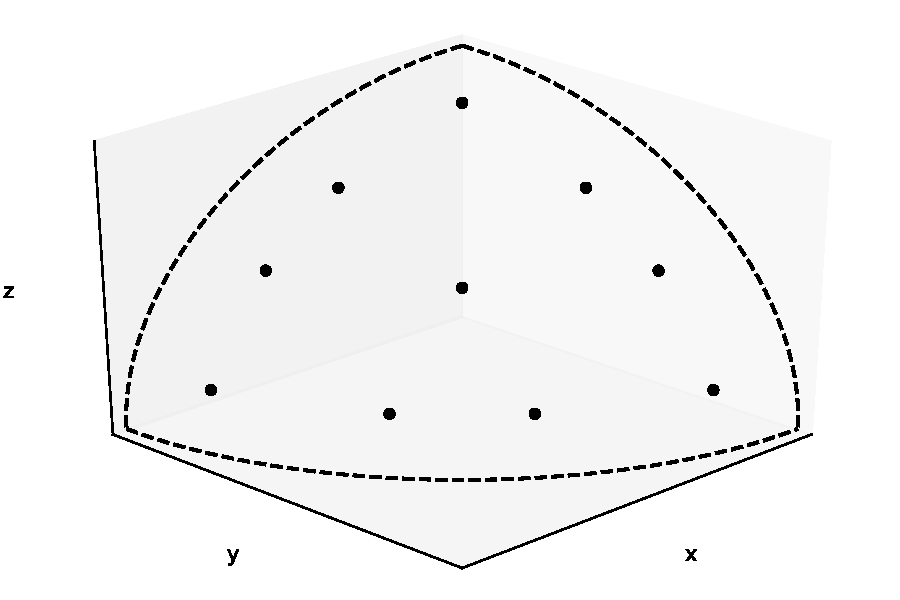
\includegraphics[width=\linewidth]{S8-Quadrature}
              \caption{Level-Symmetric Quadrature ($S_8$)}
              \label{fig:NTT:S8 Quadrature}
            \end{subfigure}%
            \hfill
            \begin{subfigure}[t]{0.45\linewidth}
              \centering
              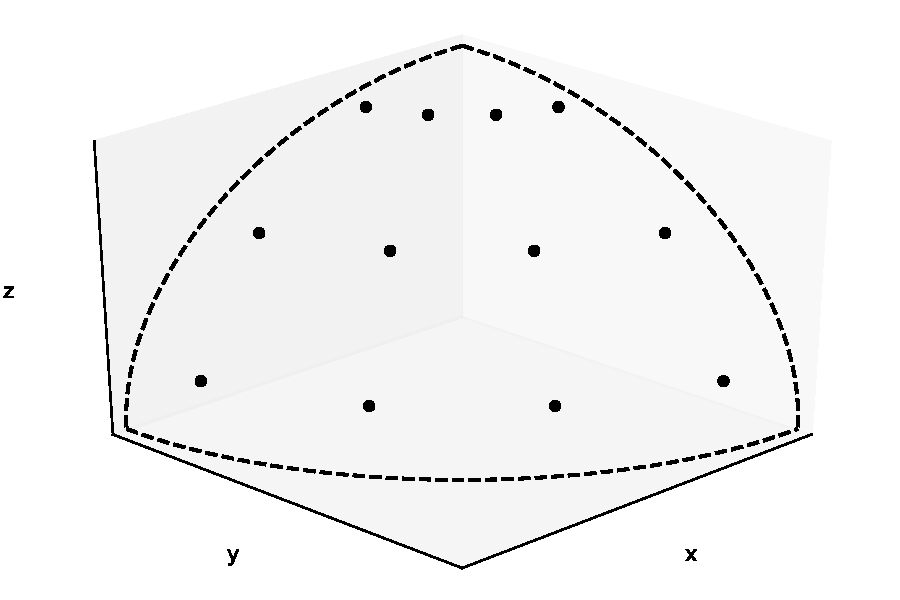
\includegraphics[width=\linewidth]{ChebyshevGauss}
              \caption{Chebyshev-Gauss Product Quadrature with 4 azimuthal and 3 polar angles}
              \label{fig:NTT:ChebyshevGauss Quadrature}
            \end{subfigure}
            \caption{(a) Level-Symmetric and (b) product quadrature direction set examples shown for a single octant of the unit-sphere.}
            \label{fig:NTT:Quadrature Examples}
          \end{figure}
        }
      }
    }
  }

  \section{State-of-the-Art 3-D Computational Transport Methods}{\label{sec:NTT:3-D Transport Methods}
    Until recently, whole-core neutronics calculations were carried out primarily through a two-step procedure.
    First, a transport method was used to compute homogenized cross section data for assemblies, and then 3-D diffusion was used to solve the problem.
    More recently, research has focused on a one-step approach, so-called direct whole-core transport.
    In this approach, the 3-D reactor is directly modeled using transport methods.
    There are many different transport methods that are currently being researched; this section seeks to give an overview of several state-of-the-art 3-D transport methods.

    \subsection{S\texorpdfstring{$P_N$}{PN}}{\label{ssec:3T:SPN}
      \DeclareDocumentCommand{\xstr}{ m }{\CrossSection_{tr,#1}}
      \DeclareDocumentCommand{\xsa}{}{\CrossSection_{a}}
      \DeclareDocumentCommand{\xst}{}{\CrossSection_{t}}
      \DeclareDocumentCommand{\xss}{ m }{\CrossSection_{s,#1}}
      \DeclareDocumentCommand{\fluxm}{ m }{ \phi_{#1} }
      \DeclareDocumentCommand{\Q}{}{Q}
      \DeclareDocumentCommand{\D}{}{D}

      The \acf{SPN} method was introduced by \citet{SPN} in 1961, and was seen as a middle ground between diffusion and transport \cite{Mcclarren2010}.
      The \ac{SPN} equations were first derived by examining the form of the 1-D \ac{PN} equations; in fact, the 1-D \ac{SPN} and \ac{PN} equations are equivalent.
      While the original derivation \citet{SPN} lacked theoretical justification, the \ac{SPN} method has since been shown to be an asymptotic correction to standard diffusion theory \cite{Larsen2010}.

      The mono-energetic planar geometry \ac{PN} equations can be written as
      \begin{subequations}\label[subeqs]{eqs:eqs}
        \begin{equation}\label{eq:SPN:Planar PN}
          \deriv{}{z}\left[\frac{l}{2l+1}\fluxm{l-1} + \frac{l+1}{2l+1}\fluxm{l+1}\right] + \xst\fluxm{l} = \xss{l}\fluxm{l} + \Q\delta_{l,0}, \quad\text{for}\quad 0\leq l\leq N,
        \end{equation}
        where $\xss{l}$ is the lth order scattering moment and $\Q$ is either an external source or fission source.
      \end{subequations}
      The expansion is generally truncated by assuming that $\fluxm{N+1}=0$.

      The 1-D $P_1$ equation can be written as
      \begin{equation}\label{eq:SPN:P1}
        -\deriv{}{z}\D\deriv{}{z}\fluxm{0} + \xst\fluxm{0} = \xss{0}\fluxm{0} + \Q,
      \end{equation}
      where
      \begin{equation}\label{eq:SPN:Diffusion Coefficient}
        \D \defined \frac{1}{3(\xst-\xss{1})}.
      \end{equation}
      The 3-D $P_1$ equations simply replace the derivative term operator of \cref{eq:SPN:P1} with the 3-D diffusion operator,
      \[
        \deriv{}{z}\D\deriv{}{z} \to \grad\vdot\D\grad,
      \]
      yielding the 3-D $P_1$ (diffusion) equation:
      \begin{equation}\label{eq:SPN:3D Diffusion}
        -\grad\vdot\D\grad\fluxm{0} + \xst\fluxm{0} = \xss{0}\fluxm{0} + \Q.
      \end{equation}

      This simple relation between 1-D and 3-D equations only holds for the special $P_1$ case.
      The \ac{SPN} method uses a similar modification for higher-order $P_N$ equations.
      This results in some lost accuracy compared to \ac{PN}, but the \ac{SPN} equations are significantly simpler to solve \cite{SPN,Mcclarren2010}.
      Unlike \ac{PN}, \ac{SPN} equations do not converge to the transport solution as $N\to\infty$, but they do generally have higher accuracy than diffusion (for orders of $N > 1$).
      Generally, S$P_3$ or S$P_5$ are considered to have sufficient accuracy, and are generally less computationally intensive than transport methods.

      The mono-energetic \ac{SPN} equations can be written as
      \begin{subequations}\label[subeqs]{eqs:SPN:SPN}
        \begin{equation}\label{eq:SPN:SPN 0}
          -\grad\vdot\frac{1}{3\xstr{1}}\grad\fluxm{0} -\grad\vdot\frac{2}{3\xstr{1}}\grad\fluxm{2} + \xstr{0}\fluxm{0} = \Q,
        \end{equation}
        \begin{aequation}\label{eq:SPN:SPN N}
          &-\grad\vdot\left(\frac{n(n-1)}{(2n+1)(2n-1)\xstr{n-1}}\right)\grad\fluxm{n-2}\\
          &-\grad\vdot\left(\frac{(n+1)(n+2)}{(2n+1)(2n+3)\xstr{n+1}}\right)\grad\fluxm{n+2}\\
          &-\grad\vdot\left(\frac{n^2}{(2n+1)(2n-1)\xstr{n-1}} + \frac{(n+1)^2}{(2n+1)(2n+3)\xstr{n+1}}\right)\grad\fluxm{n}\\
          &+\xstr{n}\fluxm{n} = 0, \quad{\text{for}\quad n=2,4,...,N-1},
        \end{aequation}
        where
        \begin{equation}\label{eq:SPN:xstr}
          \xstr{n} \defined \CrossSection_t - \CrossSection_{s,n}.
        \end{equation}
      \end{subequations}

      % [CURRENT RESEARCH]
    }

    \subsection{Method of Characteristics}{\label{ssec:3T:Method of Characteristics}
      The \acf{MOC} is a technique used to solve first-order \acp{PDE}, by transforming the \ac{PDE} into a system of \acp{ODE}.
      The method was first applied to the neutron transport problem by \citeauthor{Askew1972} in 1972 \cite{Askew1972}, but it only began to see real use in the 1980's \cite{Halsall1980}.
      The \ac{MOC} transforms the transport equation into the characteristic form, by examining the equation along straight neutron paths through the spatial domain.
      By examining the equation along one of these characteristic ``tracks'' or ``rays'', the average angular flux along the track within a cell can be calculated.
      The scalar flux can then be found by collecting the average angular flux along all tracks passing through this region, in a numerical integration over space and angle.

      Like the \ac{CP} method, \ac{MOC} is able to handle completely arbitrary geometry; however, unlike the \ac{CP} method, it is also able to account for anisotropic scattering in a straightforward manner.
      Additionally, the \ac{MOC} does not produce the large matrices in realistic applications as the \ac{CP} method does.
      For problems that contain more than a few hundred cells, the \ac{MOC} is generally preferred over \ac{CP} methods \cite{Hebert2010}.

      The \ac{CDP} is a method similar to both \ac{CP} method and the \ac{MOC} \cite{Hong1999,Liu2014}.
      The \ac{CDP} uses ray-tracing to evaluate transmission probabilities between cells.
      However, it only considers transmission probabilities between cells that are traversed by a shared characteristic ray, rather than considering the transmission probability between all cells as in the \ac{CP} methods.
      This significantly reduces the computational resources required by traditional \ac{CP} methods.
      This method has also shown improvements over \ac{MOC} in cases with few unique geometries and constant material properties throughout the simulation; however these conditions are not applicable in problems of interest to industry.

      \ac{MOC} has seen extensive use as a 2-D transport method in lattice codes \cite{CASMO-4,Ferrer2016}, and as a radial transport method in 2D/1D method \cite{MPACT2016,Collins2016,DeCART,Lee2006}.
      However, due to the large number of segments generated by 3-D ray-tracing, the \ac{MOC} has been viewed as too expensive for realistic applications \cite{Sanchez2012}.
      Nonetheless, 3-D \ac{MOC} is typically seen as the ``gold-standard'' of transport methods due to its general treatment of geometry, ability to handle anisotropic scattering, and accuracy.
      For this reason, there has been active research on improving the 3-D \ac{MOC}.

      \citet{Kochunas2013} developed a hybrid shared/distributed parallel algorithm for 3-D \ac{MOC}.
      This contribution significantly increased the ability to parallelize 3-D \ac{MOC} on modern computer clusters, and showed good parallel scaling on thousands of cores.
      Other works investigated the \acf{LSA} for 3-D \ac{MOC} applications \cite{Gunow2018}, which reduces the number of segments generated during ray-tracing.
      \citet{Sciannandrone2016} developed optimized tracking strategies (chord-classification) for locally extruded geometries for 3-D \ac{MOC} calculations.
      These optimized strategies did not reduce the number of tracks or segments generated, but they significantly reduced the memory required to store them.
      Still, 3-D \ac{MOC} remains too expensive for usage outside work in academia or national laboratories.

      The \ac{MOC} is the primary subject of this thesis work.
      \Cref{ch:The Method of Characteristics} is devoted to the details of the method, and \cref{sec:MOC:Ray-Tracing} expands upon the details of current ray-tracing techniques used in \ac{MOC}.
      \Cref{ch:Improved Linear Source Formulation for Multi-physics and 2D/1D Applications} details improvements made to the \ac{MOC} in this thesis work, and \cref{ch:MacroRay} describes a newly investigated ray-tracing method.
    }

    % Here just to make sure previous macros didn't screw anything up
    %%% Multi-group Energy quantities %%%
\DeclareDocumentCommand{\gprime}{}{g^{\prime}}
% Cross-sections
\DeclareDocumentCommand{\xs}{ O{t} O{\loc} O{g}}{\ensuremath{\CrossSection_{#1}^{#3}(#2)}}
\DeclareDocumentCommand{\xst}{ O{\loc} O{g} }{\xs[t][#1][#2]}
\DeclareDocumentCommand{\xsa}{ O{\loc} O{g} }{\xs[a][#1][#2]}
\DeclareDocumentCommand{\xsf}{ O{\loc} O{\gprime} }{\xs[f][#1][#2]}
\DeclareDocumentCommand{\xss}{ o O{\loc} O{\dirprime\vdot\dir} O{\gprime \to g} }{
    \IfNoValueOrEmptyTF{#1}
    {\xs[s][#2,#3][#4]}
    {\xs[s,#1][#2][#4]}
}
\DeclareDocumentCommand{\spect}{ O{\loc} O{g} }{\ensuremath{\Spectrum^{#2}(#1)}}
\DeclareDocumentCommand{\nufis}{ O{\loc} O{\gprime} }{ \ensuremath{\nu\xsf[#1][#2]}}
\DeclareDocumentCommand{\D}{ O{\loc} O{g} }{\ensuremath{D^{#2}(#1)}}

% Flux
\DeclareDocumentCommand{\aflux}{ O{\loc} O{\dir} O{g} }{\ensuremath{\AngularFlux^{#3}(#1,#2)}}
\DeclareDocumentCommand{\sflux}{ O{\loc} O{\gprime} }{\ensuremath{\ScalarFlux^{#2}(#1)}}
\DeclareDocumentCommand{\current}{ O{\loc} O{g} }{\ensuremath{\Current^{#2}(#1)}}
\DeclareDocumentCommand{\fluxmoma}{ O{\ell} O{n} O{\loc} O{g} }{\ensuremath{\ScalarFlux^{#2,#4}_{#1}(#3)}}

% Source
\DeclareDocumentCommand{\source}{ O{\loc} O{\dir} O{g} }{\ensuremath{q^{#3}(#1,#2)}}
\DeclareDocumentCommand{\sourcemoma}{ O{\ell} O{n} O{\loc} O{g} }{\ensuremath{q^{#2,#4}_{#1}(#3)}}

    %%% Discrete Ordinates Quantities %%%
\DeclareDocumentCommand{\mprime}{}{m^{\prime}}
\DeclareDocumentCommand{\dirm}{ O{m} }{\dir_{#1}}
\DeclareDocumentCommand{\wt}{ O{m} }{\Weight_{#1}}

% Quadrature set
\DeclareDocumentCommand{\angquad}{ O{N} }{ \mathcal{M}_{#1} }

% Cross-Sections
\DeclareDocumentCommand{\xss}{ o O{\loc} O{ m^{\prime}\!\to m} O{\gprime\!\to g} }{
    \IfNoValueOrEmptyTF{#1}
    {\xs[s,#3][#2][#4]}
    {\xs[s,#1][#2][#4]}
}

% Flux
\DeclareDocumentCommand{\aflux}{ O{\loc} O{m} O{g}}{\ensuremath{\AngularFlux^{#3}_{#2}\!\left(#1\right)}}

% Source
\DeclareDocumentCommand{\source}{ O{\loc} O{m} O{g} }{\ensuremath{q^{#3}_{#2}\!\left(#1\right)}}

    %%% MOC quantities %%%
% Geometric
\DeclareDocumentCommand{\Length}{}{s}
\DeclareDocumentCommand{\NormalizedLength}{}{t}
\DeclareDocumentCommand{\len}{ O{} }{\Length_{#1}}
\DeclareDocumentCommand{\segl}{ O{mki} }{\Length_{#1}}
\DeclareDocumentCommand{\nlen}{ O{m} }{\NormalizedLength_{#1}}
\DeclareDocumentCommand{\nsegl}{ O{mki} }{\NormalizedLength_{#1}}

\DeclareDocumentCommand{\centroid}{ O{\loc} O{i} }{#1_{#2}^{\text{c}}}
\DeclareDocumentCommand{\locIn}{ O{\loc} O{mki} }{{#1}_{#2}^{\text{in}}}
\DeclareDocumentCommand{\locOut}{ O{\loc} O{mki} }{{#1}_{#2}^{\text{out}}}
\DeclareDocumentCommand{\locCent}{ O{\loc} O{mki} }{{#1}_{#2}^{\text{c}}}
\DeclareDocumentCommand{\M}{ o O{i}}{%
    \IfNoValueOrEmptyTF{#1}
        {\vec{M}_{#2}}
        {M_{#2,#1}}
}
\DeclareDocumentCommand{\C}{o O{i} O{g}}{%
    \IfNoValueOrEmptyTF{#1}
        {\vec{C}_{#2}^{#3}}
        {C_{#2,#1}^{#3}}
}


% Integration
\DeclareAutoPairedDelimiter{\MOCTrackIntegral}{\langle}{\rangle_{mki}}
\DeclareAutoPairedDelimiter{\MOCSingleAngleIntegral}{\langle}{\rangle_{mi}}
\DeclareAutoPairedDelimiter{\MOCIntegral}{\langle}{\rangle_{i}}

% Cross-sections
\DeclareDocumentCommand{\xs}{ O{t} O{i} O{g}}{\ensuremath{\CrossSection_{#1,#2}^{#3}}}
\DeclareDocumentCommand{\xst}{ O{i} O{g} }{\xs[t][#1][#2]}
\DeclareDocumentCommand{\xsa}{ O{i} O{g} }{\xs[a][#1][#2]}
\DeclareDocumentCommand{\xsf}{ O{i} O{\gprime} }{\xs[f][#1][#2]}
\DeclareDocumentCommand{\xss}{ o O{i} O{m'\to m} O{\gprime \to g} }{
    \IfNoValueOrEmptyTF{#1}
    {\xs[s][#2,#3][#4]}
    {\xs[s,#1][#2][#4]}
}

\DeclareDocumentCommand{\spect}{ O{i} O{g} }{\ensuremath{\Spectrum^{#2}_{#1}}}
\DeclareDocumentCommand{\nufis}{ O{i} O{\gprime} }{ \ensuremath{\nu\xsf[#1][#2]}}
\DeclareDocumentCommand{\D}{ O{i} O{g} }{\ensuremath{D^{#2}_{#1}}}
\DeclareDocumentCommand{\opt}{ O{m} O{g} }{\OpticalThickness_{#1}^{#2}}
\DeclareDocumentCommand{\segopt}{ O{mki} O{g} }{\opt[#1][#2]}

% MOC Parameters
\DeclareDocumentCommand{\tA}{ O{a} }{\ensuremath{\delta\!A_{#1}}}
\DeclareDocumentCommand{\Weight}{}{w}
\DeclareDocumentCommand{\wt}{ O{m} }{\Weight_{#1}}
\DeclareDocumentCommand{\wtbar}{ O{m} }{\overline{\Weight}_{#1}}
\DeclareDocumentCommand{\renorm}{ O{i} }{\ensuremath{\xi_{#1}}}

% Flux
\DeclareDocumentCommand{\aflux}{ O{mki} O{g} O{\len} }{
    \IfNoValueOrEmptyTF{#3}
    {\AngularFlux^{#2}_{#1}}
    {\ensuremath{\AngularFlux^{#2}_{#1}\!\left(#3\right)}}
}
\DeclareDocumentCommand{\afluxin}{ O{mki} O{g} }{\AngularFlux^{#2,\text{in}}_{#1}}
\DeclareDocumentCommand{\afluxout}{ O{mki} O{g} }{\AngularFlux^{#2,\text{out}}_{#1}}
\DeclareDocumentCommand{\sflux}{ O{g} O{i} }{\ScalarFlux_{#2}^{#1}}
\DeclareDocumentCommand{\current}{ O{i} O{g} }{\Current^{#2}_{#1}}
\DeclareDocumentCommand{\tfluxF}{ O{mki} O{g} }{ \overline{\AngularFlux}_{#1}^{#2} }          % Average flux-moment along track
\DeclareDocumentCommand{\tfluxL}{ O{mki} O{g} }{  \widehat{\AngularFlux}_{#1}^{#2} }          % Linear flux-moment along track
\DeclareDocumentCommand{\dflux}{ O{mki} O{g} }{ \Delta\AngularFlux_{#1}^{#2} }                % Difference of angular flux along track
\DeclareDocumentCommand{\sfluxF}{ O{i} O{g} }{ \overline{\ScalarFlux}_{#1}^{#2} }             % Average scalar flux
% \DeclareDocumentCommand{\sfluxL}{ o O{i} O{g} }{ % Linear expansion coeff (Scalar Flux)
%     \IfNoValueOrEmptyTF{#1}
%         {\lvec{\widehat{\ScalarFlux}}_{#2}^{#3}}
%         {\widehat{\ScalarFlux}_{#2,#1}^{#3}}
% }
\DeclareDocumentCommand{\sfluxL}{ O{i} O{g} o }{ % Linear expansion coeff (Scalar Flux)
    \IfNoValueOrEmptyTF{#3}
        {\lvec{\widehat{\ScalarFlux}}_{#1}^{#2}}
        {\widehat{\ScalarFlux}_{#1,#3}^{#2}}
}
% \DeclareDocumentCommand{\sfluxL}{ m O{i} O{g} }{\widehat{\ScalarFlux}_{#2,#1}^{#3} }          % Linear expansion coeff (Scalar flux)
\DeclareDocumentCommand{\afluxmom}{ O{\ell} O{n} O{i} O{\gprime} }{\FluxMoment_{#3,#1}^{#4,#2}}

% Source
\DeclareDocumentCommand{\source}{ O{mki} O{g} O{\len} }{\ensuremath{q^{#2}_{#1}\!\left(#3\right)}}
\DeclareDocumentCommand{\tsrcF}{ O{mki} O{g} }{ \overline{q}_{#1}^{#2} }          % Average source along track
\DeclareDocumentCommand{\tsrcL}{ O{mi} O{g} }{ \widehat{q}_{#1}^{#2} }          % Linear source along track
\DeclareDocumentCommand{\src}{ O{i} O{g} }{ \Source_{#1}^{#2}}                          % Generic source
\DeclareDocumentCommand{\srcF}{ O{i} O{g} }{ q_{#1}^{#2} }             % Average source
\DeclareDocumentCommand{\srcL}{ o O{i} O{g} }{ % Linear expansion coeff (Source)
    \IfNoValueOrEmptyTF{#1}
        {\lvec{\widehat{q}}_{#2}^{#3}}
        {\widehat{q}_{#2,#1}^{#3}}
}

% Linear source operators / functions
\DeclareDocumentCommand{\FluxToSource}{ O{g} }{\mathcal{S}^{#1}}

    \subsection{2D/1D Methods}{\label{ssec:3T:2D/1D Methods}
      The 2D/1D methods were first developed by researchers at \ac{KAIST} \cite{Cho2002} and \ac{KAERI} \cite{DeCART}, in the CRX and DeCART codes, respectively.
      Though different, these two methods followed the same fundamental approach to solving 3-D reactor transport problems:
      \begin{enumerate}
        \item{Divide the core into separate axial slices/planes,}
        \item{Perform 2-D transport calculations within each plane,}
        \item{Couple the planes with transverse leakages.}
      \end{enumerate}
      These methods were based on the assumption that reactors may be very heterogeneous in the radial direction, but in the axial direction they are relatively homogeneous.
      The primary difference between the two methods is in the transverse leakage terms; in CRX the transverse leakages are anisotropic, but in DeCART the leakages are isotropic.
      To distinguish these methods, they will be referred to as anisotropic and isotropic 2D/1D methods.

      Following the relative success of these methods, other research groups have followed in their paths.
      nTRACER \cite{Jung2009}, and MPACT \cite{MPACT2016} used the isotropic 2D/1D method.
      The STREAM \cite{Zheng2017}, and APOLLO3 \cite{Faure2018} have also implemented 2D/1D methods.

      \citet{Stimpson2015} implemented an anisotropic 2D/1D method in MPACT using a Fourier expansion of the azimuthal angles for the axial and radial transverse leakages.
      \citet{Jarrett2018} further improved upon \citetp{Stimpson2015} work by introducing a 2D/1D method using $P_3$ in the axial direction.
      2D/1D methods are fundamentally based on the idea that heterogeneity in the axial direction is low;
      in cases where this is not true these methods have been observed to break down, or yield solutions with larger errors.

      \DeclareDocumentCommand{\aflux}{}{\psi}
      \DeclareDocumentCommand{\xst}{ O{t} }{\Sigma_{#1}}
      \DeclareDocumentCommand{\mxst}{ O{t} }{\widetilde{\Sigma}_{#1}}
      \DeclareDocumentCommand{\dir}{}{\vec{\Omega}}
      \DeclareDocumentCommand{\rloc}{}{\loc_{xy}}
      \DeclareDocumentCommand{\TL}{}{\widetilde{J}}
      \DeclareDocumentCommand{\L}{}{\widetilde{L}}

      \subsubsection{Derivation}{\label{sssec:3T:Derivation}
        The details of the 2D/1D equations have implications on results in \cref{ch:Improved Linear Source Formulation for Multi-physics and 2D/1D Applications}.
        In this section, the 2D/1D equations are derived.
        We begin with the mono-energetic transport equation
        \begin{equation}\label{eq:2D/1D:Transport}
          \dir\vdot\grad\aflux(\loc,\dir) + \xst(\loc)\aflux(\loc,\dir) = \frac{Q(\loc)}{\fourpi},
        \end{equation}
        where $Q(\loc)$ is the source.

        2D/1D methods divide the transport equation into radial (2-D) and axial (1-D) equations.
        The streaming term, $\dir\vdot\grad\aflux$ can be divided into the radial and axial components:
        \begin{equation}\label{eq:2D/1D:Streaming Split}
          \dir\vdot\grad\aflux = (\dir\vdot\grad)_{xy}\aflux + \PolarCos\pderiv{\aflux}{z}.
        \end{equation}
        The radial equation is obtained by first separating the axial derivative from the streaming term:
        \begin{equation}\label{eq:2D/1D:Radial Eqn. 1}
          \left[(\dir\vdot\grad)_{xy} + \xst\right]\aflux(\loc,\dir) = \frac{Q(\loc)}{\fourpi} - \PolarCos\pderiv{\aflux}{z}.
        \end{equation}
        \Cref{eq:2D/1D:Radial Eqn. 1} is then integrated over an axial plane $k$, over the interval $[z_{k-1/2}, z_{k+1/2}]$, yielding
        \begin{subequations}\label[subeqs]{eqs:2D/1D:Radial Eqn.}
          \begin{equation}\label{eq:2D/1D:Radial Eqn.}
            \left[(\dir\vdot\grad)_{xy} + \xst[t,k](\rloc)\right]\aflux_k(\rloc,\dir) = \frac{Q_k(\rloc)}{\fourpi} - \TL_{z,k}(\rloc,\dir),
          \end{equation}
          where
          \begin{equation}\label{eq:2D/1D:Radial Flux}
            \aflux_k(\rloc,\dir) \defined \frac{1}{h_k}\intl[z_{k-1/2}][z_{k+1/2}]\aflux(\loc,\dir)\dif{z},
          \end{equation}
          \begin{equation}\label{eq:2D/1D:Radial Source}
            Q_k(\rloc) \defined \frac{1}{h_k}\intl[z_{k-1/2}][z_{k+1/2}]Q(\loc,\dir)\dif{z},
          \end{equation}
          \begin{equation}\label{eq:2D/1D:Axial TL}
            \TL_{z,k}(\rloc,\dir) = \frac{\PolarCos}{h_k}\left[\aflux(\rloc,z_{k+1/2},\dir) - \aflux(\rloc,z_{k-1/2})\right],
          \end{equation}
          and $h_k = z_{k+1/2}-z_{k-1/2}$.
        \end{subequations}
        Generally, the difference between isotropic and anisotropic 2D/1D methods is in the treatment of the transverse leakages, $\TL_{z,k}$.
        In MPACT, the axial transverse leakage is typically discretized over the coarse radial mesh (typically a pin cell), and is assumed to be isotropic.

        The axial equations are found by moving the radial streaming term to the right hand side of \cref{eq:2D/1D:Transport},
        \begin{equation}\label{eq:2D/1D:Axial Eqn. 1}
          \left[\PolarCos\pderiv{}{z} + \xst\right]\aflux(\loc,\dir) = \frac{Q(\loc)}{\fourpi} - (\dir\vdot\grad)_{xy}\aflux(\loc,\dir),
        \end{equation}
        and integrating over a radial area.
        This radial area can be a fine cell (transport cell), but is typically a coarser discretization such as a pin cell \cite{Jarrett2018}.
        We operate on \cref{eq:2D/1D:Axial Eqn. 1} by
        \[
          \frac{1}{A_{ij}}\intl[x_{i-1/2}][x_{i+1/2}]\intl[y_{j-1/2}][y_{j+1/2}](\vdot)\dif{x}\dif{y}
          =
          \frac{1}{A_{ij}}\iint_{ij}(\vdot)\dif{x}\dif{y},
        \]
        to obtain:
        \begin{subequations}\label[subeqs]{eqs:2D/1D:Axial}
          \begin{equation}\label{eq:2D/1D:Axial}
            \left[\PolarCos\pderiv{}{z}+\xst[t,k,ij](z,\dir)\right]\aflux_{ij}(z,\dir)
              = \frac{Q_{ij}(z)}{\fourpi} - \frac{1}{A_{ij}}\suml[s\in\{N,S,E,W\}](\dir\vdot\widehat{n}_s)\aflux_{ij,s}(z,\dir),
          \end{equation}
          where
          \begin{equation}\label{eq:2D/1D:Axial XS}
            \xst[t,k,ij](z,\dir) \defined \frac{\iint_{ij}\xst[t,k](\rloc)\aflux_k(\rloc,\dir)\dif{x}\dif{y}}{\iint_{ij}\aflux_k(\rloc,\dir)\dif{x}\dif{y}},
          \end{equation}
          where $s$ indicates a surface for the cardinal directions $\{N,S,E,W\}$.
          For hexagonal pins there would instead be six directions to loop over; for simplicity this work assumes cartesian pin cells.
        \end{subequations}
        Typically the coarse cell cross sections are taken to be isotropic, but polar dependence has been investigated \cite{Jarrett2018}.

        The radial equations, \cref{eqs:2D/1D:Radial Eqn.}, are solved by a 2-D transport method, such as \ac{MOC}, while the axial equations, \cref{eqs:2D/1D:Axial}, are solved by either a transport method or approximate method such as diffusion \cite{Collins2016,Jarrett2018}.
        The radial equations yield surface fluxes on the pin faces, while the axial equations yield surface fluxes on the axial planar faces.
        The radial equations are, however, integrated over an axial plane which results in an axial flat solution within each plane.
        These methods then require many axial planes to resolve the axial behavior in a system, particularly if there is significant axial variation in the solution.
      }

      \subsubsection{Transverse Leakage Splitting}{\label{sssec:3T:Transverse Leakage Splitting}
        \Cref{eqs:2D/1D:Radial Eqn.} give no guarantee that the right-hand-sides are positive.
        Negative sources present considerable challenges to iteration stability when using non-linear acceleration methods such as \ac{CMFD} \cite{Jarrett2018}.
        The transverse leakage splitting method \cite{Stimpson2015,Kelley2015} was developed to ``split'' the transverse leakage term such that the total source ($Q+\TL$) is non-negative.
        A split term, $\L_{z}$, is defined
        \begin{equation}\label{eq:2D/1D:Split Term}
          \L_z \defined -\left[\frac{Q_k(\rloc)}{\fourpi} - \TL_{z,k}(\rloc,\dir)\right],
        \end{equation}
        and is added to both sides of \cref{eq:2D/1D:Radial Eqn.}.
        The left hand side (the 2-D transport operator) cannot have a free-source term, so it is necessary to merge this split term into the cross section term.
        The angular flux is not known a priori, so a approximation is used, typically isotropic flux:
        \begin{equation}\label{eq:2D/1D:Isotropic Flux}
          \aflux_k(\rloc,\dir) \approx \frac{\phi_k(\rloc)}{\fourpi}.
        \end{equation}
        This approximation is introduced only to combine the left-hand-side leakage term into the cross section term as
        \begin{equation}\label{eq:2D/1D:Split XS}
          \mxst[t,k](\rloc) \defined \xst[t,k](\rloc) + \fourpi\frac{\L_z}{\phi_k(\rloc)}.
        \end{equation}
        The radial equation then becomes
        \begin{equation}\label{eq:2D/1D:Split Radial Eqn.}
          \left[(\dir\vdot\grad)_{xy} + \mxst[t,k](\rloc)\right]\aflux_k(\rloc,\dir) = 0.
        \end{equation}

        Because splitting introduces an approximation, it generally decreases the accuracy of the solution.
        Thus, the transverse splitting method is typically use only in cells that have a negative source.
        More recently, alternative methods have been investigated \cite{Zhao2018}, but they will not be covered in this work.
      }
    }

    % Here just to make sure previous macros didn't screw anything up
    %%% Multi-group Energy quantities %%%
\DeclareDocumentCommand{\gprime}{}{g^{\prime}}
% Cross-sections
\DeclareDocumentCommand{\xs}{ O{t} O{\loc} O{g}}{\ensuremath{\CrossSection_{#1}^{#3}(#2)}}
\DeclareDocumentCommand{\xst}{ O{\loc} O{g} }{\xs[t][#1][#2]}
\DeclareDocumentCommand{\xsa}{ O{\loc} O{g} }{\xs[a][#1][#2]}
\DeclareDocumentCommand{\xsf}{ O{\loc} O{\gprime} }{\xs[f][#1][#2]}
\DeclareDocumentCommand{\xss}{ o O{\loc} O{\dirprime\vdot\dir} O{\gprime \to g} }{
    \IfNoValueOrEmptyTF{#1}
    {\xs[s][#2,#3][#4]}
    {\xs[s,#1][#2][#4]}
}
\DeclareDocumentCommand{\spect}{ O{\loc} O{g} }{\ensuremath{\Spectrum^{#2}(#1)}}
\DeclareDocumentCommand{\nufis}{ O{\loc} O{\gprime} }{ \ensuremath{\nu\xsf[#1][#2]}}
\DeclareDocumentCommand{\D}{ O{\loc} O{g} }{\ensuremath{D^{#2}(#1)}}

% Flux
\DeclareDocumentCommand{\aflux}{ O{\loc} O{\dir} O{g} }{\ensuremath{\AngularFlux^{#3}(#1,#2)}}
\DeclareDocumentCommand{\sflux}{ O{\loc} O{\gprime} }{\ensuremath{\ScalarFlux^{#2}(#1)}}
\DeclareDocumentCommand{\current}{ O{\loc} O{g} }{\ensuremath{\Current^{#2}(#1)}}
\DeclareDocumentCommand{\fluxmoma}{ O{\ell} O{n} O{\loc} O{g} }{\ensuremath{\ScalarFlux^{#2,#4}_{#1}(#3)}}

% Source
\DeclareDocumentCommand{\source}{ O{\loc} O{\dir} O{g} }{\ensuremath{q^{#3}(#1,#2)}}
\DeclareDocumentCommand{\sourcemoma}{ O{\ell} O{n} O{\loc} O{g} }{\ensuremath{q^{#2,#4}_{#1}(#3)}}

    %%% Discrete Ordinates Quantities %%%
\DeclareDocumentCommand{\mprime}{}{m^{\prime}}
\DeclareDocumentCommand{\dirm}{ O{m} }{\dir_{#1}}
\DeclareDocumentCommand{\wt}{ O{m} }{\Weight_{#1}}

% Quadrature set
\DeclareDocumentCommand{\angquad}{ O{N} }{ \mathcal{M}_{#1} }

% Cross-Sections
\DeclareDocumentCommand{\xss}{ o O{\loc} O{ m^{\prime}\!\to m} O{\gprime\!\to g} }{
    \IfNoValueOrEmptyTF{#1}
    {\xs[s,#3][#2][#4]}
    {\xs[s,#1][#2][#4]}
}

% Flux
\DeclareDocumentCommand{\aflux}{ O{\loc} O{m} O{g}}{\ensuremath{\AngularFlux^{#3}_{#2}\!\left(#1\right)}}

% Source
\DeclareDocumentCommand{\source}{ O{\loc} O{m} O{g} }{\ensuremath{q^{#3}_{#2}\!\left(#1\right)}}

    %%% MOC quantities %%%
% Geometric
\DeclareDocumentCommand{\Length}{}{s}
\DeclareDocumentCommand{\NormalizedLength}{}{t}
\DeclareDocumentCommand{\len}{ O{} }{\Length_{#1}}
\DeclareDocumentCommand{\segl}{ O{mki} }{\Length_{#1}}
\DeclareDocumentCommand{\nlen}{ O{m} }{\NormalizedLength_{#1}}
\DeclareDocumentCommand{\nsegl}{ O{mki} }{\NormalizedLength_{#1}}

\DeclareDocumentCommand{\centroid}{ O{\loc} O{i} }{#1_{#2}^{\text{c}}}
\DeclareDocumentCommand{\locIn}{ O{\loc} O{mki} }{{#1}_{#2}^{\text{in}}}
\DeclareDocumentCommand{\locOut}{ O{\loc} O{mki} }{{#1}_{#2}^{\text{out}}}
\DeclareDocumentCommand{\locCent}{ O{\loc} O{mki} }{{#1}_{#2}^{\text{c}}}
\DeclareDocumentCommand{\M}{ o O{i}}{%
    \IfNoValueOrEmptyTF{#1}
        {\vec{M}_{#2}}
        {M_{#2,#1}}
}
\DeclareDocumentCommand{\C}{o O{i} O{g}}{%
    \IfNoValueOrEmptyTF{#1}
        {\vec{C}_{#2}^{#3}}
        {C_{#2,#1}^{#3}}
}


% Integration
\DeclareAutoPairedDelimiter{\MOCTrackIntegral}{\langle}{\rangle_{mki}}
\DeclareAutoPairedDelimiter{\MOCSingleAngleIntegral}{\langle}{\rangle_{mi}}
\DeclareAutoPairedDelimiter{\MOCIntegral}{\langle}{\rangle_{i}}

% Cross-sections
\DeclareDocumentCommand{\xs}{ O{t} O{i} O{g}}{\ensuremath{\CrossSection_{#1,#2}^{#3}}}
\DeclareDocumentCommand{\xst}{ O{i} O{g} }{\xs[t][#1][#2]}
\DeclareDocumentCommand{\xsa}{ O{i} O{g} }{\xs[a][#1][#2]}
\DeclareDocumentCommand{\xsf}{ O{i} O{\gprime} }{\xs[f][#1][#2]}
\DeclareDocumentCommand{\xss}{ o O{i} O{m'\to m} O{\gprime \to g} }{
    \IfNoValueOrEmptyTF{#1}
    {\xs[s][#2,#3][#4]}
    {\xs[s,#1][#2][#4]}
}

\DeclareDocumentCommand{\spect}{ O{i} O{g} }{\ensuremath{\Spectrum^{#2}_{#1}}}
\DeclareDocumentCommand{\nufis}{ O{i} O{\gprime} }{ \ensuremath{\nu\xsf[#1][#2]}}
\DeclareDocumentCommand{\D}{ O{i} O{g} }{\ensuremath{D^{#2}_{#1}}}
\DeclareDocumentCommand{\opt}{ O{m} O{g} }{\OpticalThickness_{#1}^{#2}}
\DeclareDocumentCommand{\segopt}{ O{mki} O{g} }{\opt[#1][#2]}

% MOC Parameters
\DeclareDocumentCommand{\tA}{ O{a} }{\ensuremath{\delta\!A_{#1}}}
\DeclareDocumentCommand{\Weight}{}{w}
\DeclareDocumentCommand{\wt}{ O{m} }{\Weight_{#1}}
\DeclareDocumentCommand{\wtbar}{ O{m} }{\overline{\Weight}_{#1}}
\DeclareDocumentCommand{\renorm}{ O{i} }{\ensuremath{\xi_{#1}}}

% Flux
\DeclareDocumentCommand{\aflux}{ O{mki} O{g} O{\len} }{
    \IfNoValueOrEmptyTF{#3}
    {\AngularFlux^{#2}_{#1}}
    {\ensuremath{\AngularFlux^{#2}_{#1}\!\left(#3\right)}}
}
\DeclareDocumentCommand{\afluxin}{ O{mki} O{g} }{\AngularFlux^{#2,\text{in}}_{#1}}
\DeclareDocumentCommand{\afluxout}{ O{mki} O{g} }{\AngularFlux^{#2,\text{out}}_{#1}}
\DeclareDocumentCommand{\sflux}{ O{g} O{i} }{\ScalarFlux_{#2}^{#1}}
\DeclareDocumentCommand{\current}{ O{i} O{g} }{\Current^{#2}_{#1}}
\DeclareDocumentCommand{\tfluxF}{ O{mki} O{g} }{ \overline{\AngularFlux}_{#1}^{#2} }          % Average flux-moment along track
\DeclareDocumentCommand{\tfluxL}{ O{mki} O{g} }{  \widehat{\AngularFlux}_{#1}^{#2} }          % Linear flux-moment along track
\DeclareDocumentCommand{\dflux}{ O{mki} O{g} }{ \Delta\AngularFlux_{#1}^{#2} }                % Difference of angular flux along track
\DeclareDocumentCommand{\sfluxF}{ O{i} O{g} }{ \overline{\ScalarFlux}_{#1}^{#2} }             % Average scalar flux
% \DeclareDocumentCommand{\sfluxL}{ o O{i} O{g} }{ % Linear expansion coeff (Scalar Flux)
%     \IfNoValueOrEmptyTF{#1}
%         {\lvec{\widehat{\ScalarFlux}}_{#2}^{#3}}
%         {\widehat{\ScalarFlux}_{#2,#1}^{#3}}
% }
\DeclareDocumentCommand{\sfluxL}{ O{i} O{g} o }{ % Linear expansion coeff (Scalar Flux)
    \IfNoValueOrEmptyTF{#3}
        {\lvec{\widehat{\ScalarFlux}}_{#1}^{#2}}
        {\widehat{\ScalarFlux}_{#1,#3}^{#2}}
}
% \DeclareDocumentCommand{\sfluxL}{ m O{i} O{g} }{\widehat{\ScalarFlux}_{#2,#1}^{#3} }          % Linear expansion coeff (Scalar flux)
\DeclareDocumentCommand{\afluxmom}{ O{\ell} O{n} O{i} O{\gprime} }{\FluxMoment_{#3,#1}^{#4,#2}}

% Source
\DeclareDocumentCommand{\source}{ O{mki} O{g} O{\len} }{\ensuremath{q^{#2}_{#1}\!\left(#3\right)}}
\DeclareDocumentCommand{\tsrcF}{ O{mki} O{g} }{ \overline{q}_{#1}^{#2} }          % Average source along track
\DeclareDocumentCommand{\tsrcL}{ O{mi} O{g} }{ \widehat{q}_{#1}^{#2} }          % Linear source along track
\DeclareDocumentCommand{\src}{ O{i} O{g} }{ \Source_{#1}^{#2}}                          % Generic source
\DeclareDocumentCommand{\srcF}{ O{i} O{g} }{ q_{#1}^{#2} }             % Average source
\DeclareDocumentCommand{\srcL}{ o O{i} O{g} }{ % Linear expansion coeff (Source)
    \IfNoValueOrEmptyTF{#1}
        {\lvec{\widehat{q}}_{#2}^{#3}}
        {\widehat{q}_{#2,#1}^{#3}}
}

% Linear source operators / functions
\DeclareDocumentCommand{\FluxToSource}{ O{g} }{\mathcal{S}^{#1}}

    \subsection{Extruded 3-D Methods}{\label{ssec:3T:Extruded 3-D Methods}
      Due to the wide adoption of 2D/1D methods in recent years, some current research paths have turned towards \emph{extruded mesh} 3-D transport methods.
      An axially extruded mesh is a mesh that uses the same radial discretization for all axial positions in the domain.
      These methods generally rely on the mesh of the problem to be an axially extruded mesh, and use 3-D transport methods that rely on that assumption.
      This an active area of research and while they usually rely on similar assumptions, many different approaches have been taken.

      The PROTEUS \cite{Marin-Lafleche2013} code introduced a new transport methodology that combined 2-D \ac{MOC} with a discontinuous Galerkin method (finite-elements) for treatment of the axial variable.
      Other groups have used similar approaches, but with different axial basis functions; STREAM \cite{Zheng2017} uses linear orthogonal functions, and recent work at \ac{UM} \cite{HerringExtruded} has utilized the Legendre polynomials.
      Recent work on STREAM has used a diamond-difference method for approximating axial behavior.% [CITATION].
      Generally, these methods do not suffer from the same inaccuracies of standard 2D/1D methods, but they do still assume the use of extruded meshes.

      The \acf{LEAF} method, developed by \citet{Yamamoto2017} in the GENESIS code, is an extruded method that is distinct from the PROTEUS-like methods.
      This method is the successor of the ASMOC3D method \cite{Giho2008}.
      The \ac{LEAF} method performs 2-D radial ray-tracing to generate a set of characteristic planes.
      The angular flux on the left, right, top, and bottom surfaces of each characteristic plane is given an assumed shape as a linear combination of Legendre polynomials.
      A transport calculation is then carried out in each of these characteristic planes by the method of short characteristics.

      The extruded 3-D transport methods seem to have accuracy benefits over the more traditional 2D/1D methods;
        however, they are usually more computationally expensive, though reducing this cost is an active area of research.
      Unlike general 3-D transport methods, such as 3-D \ac{MOC}, these extruded methods are unable to handle general geometries.
      This may be of concern in future reactor designs, but in most modern reactor designs this is an appropriate simplification to make.
    }
  }

  \section{Source Iteration}{\label{sec:NTT:Source Iteration}
    Generally, the $k$-eigenvalue transport problems, introduced in \cref{sec:NTT:k-Eigenvalue Problems}, are solved iteratively.
    Given an initial guess for the $k$-eigenvalue, boundary conditions, and interior flux-moments, an estimate of the source can be computed.
    A transport ``sweep'' can be performed, in which updated boundary conditions and flux-moments are computed.
    Given these updated flux-moments a new estimate of the eigenvalue can be calculated.
    This process can be repeated until the eigenvalue and flux-moments are converged within some tolerance.
    This procedure is referred to as either source iteration, or power iteration; typically, power iteration is used to refer to this procedure in problems with a fixed source.
    For simplicity, this process is shown for a isotropic mono-energetic, continuous-space, one-dimensional transport problem in \cref{alg:NTT:Source Iteration}.

    \begin{algorithm}[ht]
      \centering
      \caption{Source Iteration algorithm for the $k$-eigenvalue transport problem.}
      \label{alg:NTT:Source Iteration}
      \begin{algorithmic}[1]
        \State{Begin iteration $j$ with a known boundary conditions, scalar flux estimate, $\ScalarFlux^{(j)}(x)$, and a $k$-eigenvalue estimate, $\keff^{j}$.}
        \State{Perform a transport sweep:
          \begin{subequations}\label[subeqs]{eqs:NTT:Source Iteration:Transport Sweep}
            \begin{equation}\label{eq:NTT:Source Iteration:Transport Sweep}
              \left[\PolarCos\pderiv{}{x} + \CrossSection_t(x)\right]\AngularFlux^{(j+1)}(x,\PolarCos) = \frac{1}{2}\left[\CrossSection_s(x) + \frac{1}{\keff^{(j)}}\nu\CrossSection_f(x)\right]\ScalarFlux^{(j)}(x),
            \end{equation}
            \begin{equation*}
              \forall x\in [0,X], \quad \forall\PolarCos \in [-1, 1],
            \end{equation*}
            \begin{equation}\label{eq:NTT:Source Iteration:BC-Left}
              \AngularFlux^{(j)}(0,\PolarCos) = \AngularFlux^b(\PolarCos), \quad \PolarCos\in[0,1],
            \end{equation}
            \begin{equation}\label{eq:NTT:Source Iteration:BC-Right}
              \AngularFlux^{(j)}(X,\PolarCos) = \AngularFlux^b(\PolarCos), \quad \PolarCos\in[-1,0].
            \end{equation}
          \end{subequations}
        }
        \State{Update the scalar flux, and the eigenvalue for the next iteration:
          \begin{subequations}\label[subeqs]{eqs:NTT:Source Iteration:Update}
            \begin{equation}\label{eq:NTT:Source Iteration:Scalar Flux Update}
              \ScalarFlux^{(j+1)}(x) = \left(\intl[-1][1]\AngularFlux^{(j+1)}(x,\PolarCos)\dif{\PolarCos}\right) \frac{\Phi_0}{\frac{1}{X}\intl[0][X]\intl[-1][1]\AngularFlux^{(j+1)}(x',\PolarCos)\dif{\PolarCos}\dif{x'}},
            \end{equation}
            \begin{equation}\label{eq:NTT:Source Iteration:Eigenvalue Update}
              \keff^{(j+1)} = \frac{\intl[0][X]\nu\CrossSection_f\ScalarFlux^{(j+1)}(x)\dif{x}}{\intl[0][X]\CrossSection_a\ScalarFlux^{(j+1)}(x)\dif{x} + \intl[-1][0]\AngularFlux^{(j+1)}(0,\PolarCos)\dif{\PolarCos}  + \intl[0][1]\AngularFlux^{(j+1)}(X,\PolarCos)\dif{\PolarCos}}.
            \end{equation}
          \end{subequations}
        }
        \State{Repeat steps 1. - 3. until sufficient convergence.}
      \end{algorithmic}
    \end{algorithm}

    \subsection{Transport Acceleration}{\label{ssec:NTT:Transport Acceleration}
      While \cref{alg:NTT:Source Iteration} is valid, it typically converges very slowly, requiring many iterations to obtain reasonable results.
      In full-core calculations, a single transport sweep is typically the most computationally expensive operation. For this reason, solving practical problems using \cref{alg:NTT:Source Iteration} is not feasible.
      There has been considerable effort in developing methods that accelerate the convergence of transport calculations by using a lower-order calculation, typically based on the diffusion approximation.
      These methods often reduce the number of iterations from O(1000) to O(10) for thermal reactor systems.

      While other acceleration methods exist \cite{Hebert2017}, the most common for $k$-eigenvalue problems are \ac{NDA} methods \cite{Smith2002}, typically using the \ac{CMFD} method \cite{Smith1983}.
      \Cref{alg:NTT:NDA} lists the standard \ac{NDA} algorithm for a 1-D mono-energetic $k$-eigenvalue problem.
      The primary difference between \ac{CMFD} and \ac{NDA} is that \ac{CMFD} introduces the concept of a second, coarser spatial grid, while \ac{NDA} uses the same spatial mesh as the transport problem.

      The \ac{CMFD} acceleration method has been shown to significantly reduce computational transport run-times \cite{Smith2002,Anistratov2011,Collins2016}.
      There have been several improvements upon the original \ac{CMFD} formulation \cite{Smith1983}, such as p\ac{CMFD} \cite{Cho2002} and od\ac{CMFD} \cite{Zhu2016}.
      The p\ac{CMFD} method preserves partial currents rather than net currents, and has been shown to be unconditionally stable for transport problems at fixed conditions \cite{Cho2002}.
      The od\ac{CMFD} method generalizes the \ac{CMFD} and p\ac{CMFD} methods by adding an artificial term to the diffusion coefficient, and has faster convergence properties than p\ac{CMFD} \cite{Zhu2016}.
      Recently, it was shown that the theoretical reason for this is the that most \ac{MOC} methods do not preserve the linear solutions of the transport equation, resulting in the need for an unphysical correction to the diffusion coefficient to account for truncation error in the transport discretization.

      Utilization of \ac{CMFD} acceleration in transport calculations with \ac{TH} feedback has not had the favorable stability and convergence properties as calculations without feedback \cite{Kochunas2017}.
      Many transport codes have required under-relaxation of the scalar flux in the iteration schemes for stability in these calculations; there is ongoing research investigating a less ad-hoc approach \cite{Kochunas2017}.
      This instability and convergence slow-down in problems with feedback has prevented full utilization of more advanced multi-level solvers \cite{Kochunas2017,Yee2018a}.

      \begin{algorithm}
        \caption{Non-linear Diffusion Acceleration (NDA) algorithm for the $k$-eigenvalue transport problem.}
        \label{alg:NTT:NDA}
        \newcommand{\ndaCurrent}[1][j]{J^{(#1)}(x)}
        \newcommand{\ndaFlux}[1][j]{\ScalarFlux^{(#1)}(x)}
        \newcommand{\ndaXST}{\CrossSection_{t}(x)}
        \newcommand{\ndaXSA}{\CrossSection_{a}(x)}
        \newcommand{\ndaNUFIS}{\nu\CrossSection_{f}(x)}
        \newcommand{\ndaD}{\frac{1}{3\ndaXST}}
        \newcommand{\ndaDHAT}{\widehat{D}^{(j)}(x)}

        \begin{algorithmic}[1]
          \State{Begin iteration $i$ with known boundary conditions, scalar flux estimate, $\ScalarFlux^{(j)}(x)$, a net current estimate, $\Current^{(j)}(x)$, and a $k$-eigenvalue estimate, $\keff$.}
          \State{Compute linear and non-linear correction factors for low-order diffusion equation:
            \begin{equation}\label{eq:NTT:NDA:Dhat}
              \ndaDHAT = \frac{\deriv{}{x}\left[\ndaCurrent + \ndaD\deriv{\ndaFlux}{x}\right]}{\ndaFlux}
            \end{equation}
          }
          \State{Solve the low-order diffusion eigenvalue problem:
            \begin{equation}\label{eq:NTT:NDA:NDA Equation}
              -\deriv{}{x}\ndaD\deriv{\ndaFlux[j+1/2]}{x}
              +\left[\ndaXSA + \ndaDHAT\right]\ndaFlux[j+1/2] = \frac{1}{\keff}\ndaNUFIS\ndaFlux[j+1/2].
            \end{equation}
          }
          \State{Perform a transport sweep using the scalar flux, and eigenvalue estimates from the low-order diffusion calculation:
            \begin{equation}\label{eq:NTT:NDA:Transport Sweep}
              \left[\PolarCos\pderiv{}{x} + \ndaXST\right]\AngularFlux^{(j+1)}(x,\PolarCos) = \frac{1}{2}\left[\CrossSection_s(x) + \frac{1}{\keff^{(j)}}\nu\CrossSection_f(x)\right]\ScalarFlux^{(j)}(x),
            \end{equation}
            \begin{equation*}
              \forall x\in [0,X], \quad \forall\PolarCos \in [-1, 1].
            \end{equation*}
          }
          \State{Update the scalar flux, current, and eigenvalue estimates for next iteration:
            \begin{subequations}\label[subeqs]{eqs:NTT:NDA:Update}
              \begin{equation}\label{eq:NTT:NDA:Scalar Flux Update}
                \ScalarFlux^{(j+1)}(x) = \intl[-1][1]\AngularFlux^{(j+1)}(x,\PolarCos)\dif{\PolarCos} \frac{\Phi_0}{\frac{1}{X}\intl[0][X]\intl[-1][1]\AngularFlux^{(j+1)}(x',\PolarCos)\dif{\PolarCos}\dif{x'}},
              \end{equation}
              \begin{equation}\label{eq:NTT:NDA:Current Update}
                \Current^{(j+1)}(x) = \intl[-1][1]\PolarCos\AngularFlux^{(j+1)}(x,\PolarCos)\dif{\PolarCos} \frac{\Phi_0}{\frac{1}{X}\intl[0][X]\intl[-1][1]\AngularFlux^{(j+1)}(x',\PolarCos)\dif{\PolarCos}\dif{x'}},
              \end{equation}
              \begin{equation}\label{eq:NTT:NDA:Eigenvalue Update}
                \keff^{(j+1)} = \frac{\intl[0][X]\nu\CrossSection_f\ScalarFlux^{(j+1)}(x)\dif{x}}{\intl[0][X]\CrossSection_a\ScalarFlux^{(j+1)}(x)\dif{x} + \intl[-1][0]\AngularFlux^{(j+1)}(0,\PolarCos)\dif{\PolarCos}  + \intl[0][1]\AngularFlux^{(j+1)}(X,\PolarCos)\dif{\PolarCos}}.
              \end{equation}
            \end{subequations}
          }
        \end{algorithmic}
      \end{algorithm}
    }
  }

  % References
  \printbibliography
}
    \chapter{The Method of Characteristics}{\label{ch:The Method of Characteristics}
    %%% Multi-group Energy quantities %%%
\DeclareDocumentCommand{\gprime}{}{g^{\prime}}
% Cross-sections
\DeclareDocumentCommand{\xs}{ O{t} O{\loc} O{g}}{\ensuremath{\CrossSection_{#1}^{#3}(#2)}}
\DeclareDocumentCommand{\xst}{ O{\loc} O{g} }{\xs[t][#1][#2]}
\DeclareDocumentCommand{\xsa}{ O{\loc} O{g} }{\xs[a][#1][#2]}
\DeclareDocumentCommand{\xsf}{ O{\loc} O{\gprime} }{\xs[f][#1][#2]}
\DeclareDocumentCommand{\xss}{ o O{\loc} O{\dirprime\vdot\dir} O{\gprime \to g} }{
    \IfNoValueOrEmptyTF{#1}
    {\xs[s][#2,#3][#4]}
    {\xs[s,#1][#2][#4]}
}
\DeclareDocumentCommand{\spect}{ O{\loc} O{g} }{\ensuremath{\Spectrum^{#2}(#1)}}
\DeclareDocumentCommand{\nufis}{ O{\loc} O{\gprime} }{ \ensuremath{\nu\xsf[#1][#2]}}
\DeclareDocumentCommand{\D}{ O{\loc} O{g} }{\ensuremath{D^{#2}(#1)}}

% Flux
\DeclareDocumentCommand{\aflux}{ O{\loc} O{\dir} O{g} }{\ensuremath{\AngularFlux^{#3}(#1,#2)}}
\DeclareDocumentCommand{\sflux}{ O{\loc} O{\gprime} }{\ensuremath{\ScalarFlux^{#2}(#1)}}
\DeclareDocumentCommand{\current}{ O{\loc} O{g} }{\ensuremath{\Current^{#2}(#1)}}
\DeclareDocumentCommand{\fluxmoma}{ O{\ell} O{n} O{\loc} O{g} }{\ensuremath{\ScalarFlux^{#2,#4}_{#1}(#3)}}

% Source
\DeclareDocumentCommand{\source}{ O{\loc} O{\dir} O{g} }{\ensuremath{q^{#3}(#1,#2)}}
\DeclareDocumentCommand{\sourcemoma}{ O{\ell} O{n} O{\loc} O{g} }{\ensuremath{q^{#2,#4}_{#1}(#3)}}

    %%% Discrete Ordinates Quantities %%%
\DeclareDocumentCommand{\mprime}{}{m^{\prime}}
\DeclareDocumentCommand{\dirm}{ O{m} }{\dir_{#1}}
\DeclareDocumentCommand{\wt}{ O{m} }{\Weight_{#1}}

% Quadrature set
\DeclareDocumentCommand{\angquad}{ O{N} }{ \mathcal{M}_{#1} }

% Cross-Sections
\DeclareDocumentCommand{\xss}{ o O{\loc} O{ m^{\prime}\!\to m} O{\gprime\!\to g} }{
    \IfNoValueOrEmptyTF{#1}
    {\xs[s,#3][#2][#4]}
    {\xs[s,#1][#2][#4]}
}

% Flux
\DeclareDocumentCommand{\aflux}{ O{\loc} O{m} O{g}}{\ensuremath{\AngularFlux^{#3}_{#2}\!\left(#1\right)}}

% Source
\DeclareDocumentCommand{\source}{ O{\loc} O{m} O{g} }{\ensuremath{q^{#3}_{#2}\!\left(#1\right)}}

    %%% MOC quantities %%%
% Geometric
\DeclareDocumentCommand{\Length}{}{s}
\DeclareDocumentCommand{\NormalizedLength}{}{t}
\DeclareDocumentCommand{\len}{ O{} }{\Length_{#1}}
\DeclareDocumentCommand{\segl}{ O{mki} }{\Length_{#1}}
\DeclareDocumentCommand{\nlen}{ O{m} }{\NormalizedLength_{#1}}
\DeclareDocumentCommand{\nsegl}{ O{mki} }{\NormalizedLength_{#1}}

\DeclareDocumentCommand{\centroid}{ O{\loc} O{i} }{#1_{#2}^{\text{c}}}
\DeclareDocumentCommand{\locIn}{ O{\loc} O{mki} }{{#1}_{#2}^{\text{in}}}
\DeclareDocumentCommand{\locOut}{ O{\loc} O{mki} }{{#1}_{#2}^{\text{out}}}
\DeclareDocumentCommand{\locCent}{ O{\loc} O{mki} }{{#1}_{#2}^{\text{c}}}
\DeclareDocumentCommand{\M}{ o O{i}}{%
    \IfNoValueOrEmptyTF{#1}
        {\vec{M}_{#2}}
        {M_{#2,#1}}
}
\DeclareDocumentCommand{\C}{o O{i} O{g}}{%
    \IfNoValueOrEmptyTF{#1}
        {\vec{C}_{#2}^{#3}}
        {C_{#2,#1}^{#3}}
}


% Integration
\DeclareAutoPairedDelimiter{\MOCTrackIntegral}{\langle}{\rangle_{mki}}
\DeclareAutoPairedDelimiter{\MOCSingleAngleIntegral}{\langle}{\rangle_{mi}}
\DeclareAutoPairedDelimiter{\MOCIntegral}{\langle}{\rangle_{i}}

% Cross-sections
\DeclareDocumentCommand{\xs}{ O{t} O{i} O{g}}{\ensuremath{\CrossSection_{#1,#2}^{#3}}}
\DeclareDocumentCommand{\xst}{ O{i} O{g} }{\xs[t][#1][#2]}
\DeclareDocumentCommand{\xsa}{ O{i} O{g} }{\xs[a][#1][#2]}
\DeclareDocumentCommand{\xsf}{ O{i} O{\gprime} }{\xs[f][#1][#2]}
\DeclareDocumentCommand{\xss}{ o O{i} O{m'\to m} O{\gprime \to g} }{
    \IfNoValueOrEmptyTF{#1}
    {\xs[s][#2,#3][#4]}
    {\xs[s,#1][#2][#4]}
}

\DeclareDocumentCommand{\spect}{ O{i} O{g} }{\ensuremath{\Spectrum^{#2}_{#1}}}
\DeclareDocumentCommand{\nufis}{ O{i} O{\gprime} }{ \ensuremath{\nu\xsf[#1][#2]}}
\DeclareDocumentCommand{\D}{ O{i} O{g} }{\ensuremath{D^{#2}_{#1}}}
\DeclareDocumentCommand{\opt}{ O{m} O{g} }{\OpticalThickness_{#1}^{#2}}
\DeclareDocumentCommand{\segopt}{ O{mki} O{g} }{\opt[#1][#2]}

% MOC Parameters
\DeclareDocumentCommand{\tA}{ O{a} }{\ensuremath{\delta\!A_{#1}}}
\DeclareDocumentCommand{\Weight}{}{w}
\DeclareDocumentCommand{\wt}{ O{m} }{\Weight_{#1}}
\DeclareDocumentCommand{\wtbar}{ O{m} }{\overline{\Weight}_{#1}}
\DeclareDocumentCommand{\renorm}{ O{i} }{\ensuremath{\xi_{#1}}}

% Flux
\DeclareDocumentCommand{\aflux}{ O{mki} O{g} O{\len} }{
    \IfNoValueOrEmptyTF{#3}
    {\AngularFlux^{#2}_{#1}}
    {\ensuremath{\AngularFlux^{#2}_{#1}\!\left(#3\right)}}
}
\DeclareDocumentCommand{\afluxin}{ O{mki} O{g} }{\AngularFlux^{#2,\text{in}}_{#1}}
\DeclareDocumentCommand{\afluxout}{ O{mki} O{g} }{\AngularFlux^{#2,\text{out}}_{#1}}
\DeclareDocumentCommand{\sflux}{ O{g} O{i} }{\ScalarFlux_{#2}^{#1}}
\DeclareDocumentCommand{\current}{ O{i} O{g} }{\Current^{#2}_{#1}}
\DeclareDocumentCommand{\tfluxF}{ O{mki} O{g} }{ \overline{\AngularFlux}_{#1}^{#2} }          % Average flux-moment along track
\DeclareDocumentCommand{\tfluxL}{ O{mki} O{g} }{  \widehat{\AngularFlux}_{#1}^{#2} }          % Linear flux-moment along track
\DeclareDocumentCommand{\dflux}{ O{mki} O{g} }{ \Delta\AngularFlux_{#1}^{#2} }                % Difference of angular flux along track
\DeclareDocumentCommand{\sfluxF}{ O{i} O{g} }{ \overline{\ScalarFlux}_{#1}^{#2} }             % Average scalar flux
% \DeclareDocumentCommand{\sfluxL}{ o O{i} O{g} }{ % Linear expansion coeff (Scalar Flux)
%     \IfNoValueOrEmptyTF{#1}
%         {\lvec{\widehat{\ScalarFlux}}_{#2}^{#3}}
%         {\widehat{\ScalarFlux}_{#2,#1}^{#3}}
% }
\DeclareDocumentCommand{\sfluxL}{ O{i} O{g} o }{ % Linear expansion coeff (Scalar Flux)
    \IfNoValueOrEmptyTF{#3}
        {\lvec{\widehat{\ScalarFlux}}_{#1}^{#2}}
        {\widehat{\ScalarFlux}_{#1,#3}^{#2}}
}
% \DeclareDocumentCommand{\sfluxL}{ m O{i} O{g} }{\widehat{\ScalarFlux}_{#2,#1}^{#3} }          % Linear expansion coeff (Scalar flux)
\DeclareDocumentCommand{\afluxmom}{ O{\ell} O{n} O{i} O{\gprime} }{\FluxMoment_{#3,#1}^{#4,#2}}

% Source
\DeclareDocumentCommand{\source}{ O{mki} O{g} O{\len} }{\ensuremath{q^{#2}_{#1}\!\left(#3\right)}}
\DeclareDocumentCommand{\tsrcF}{ O{mki} O{g} }{ \overline{q}_{#1}^{#2} }          % Average source along track
\DeclareDocumentCommand{\tsrcL}{ O{mi} O{g} }{ \widehat{q}_{#1}^{#2} }          % Linear source along track
\DeclareDocumentCommand{\src}{ O{i} O{g} }{ \Source_{#1}^{#2}}                          % Generic source
\DeclareDocumentCommand{\srcF}{ O{i} O{g} }{ q_{#1}^{#2} }             % Average source
\DeclareDocumentCommand{\srcL}{ o O{i} O{g} }{ % Linear expansion coeff (Source)
    \IfNoValueOrEmptyTF{#1}
        {\lvec{\widehat{q}}_{#2}^{#3}}
        {\widehat{q}_{#2,#1}^{#3}}
}

% Linear source operators / functions
\DeclareDocumentCommand{\FluxToSource}{ O{g} }{\mathcal{S}^{#1}}
    \def\figpath{chapters/MOC/figures/}
    \graphicspath{ {\figpath} }

    \section{Fundamentals}{\label{sec:MOC:Fundamentals}
        The \acf{MOC} is a technique used in mathematics to solve \acp{PDE}, by transforming a \ac{PDE} into a system of \acp{ODE}.
        The method was first applied to the neutron transport equation by \citeauthor{Askew1972} in 1972 \cite{Askew1972}, but only began to see real use in the 1980's \cite{Halsall1980}.
        The \ac{MOC} transforms the transport equation into the characteristic form, by following the equation along straight neutron paths through the spatial domain.
        For brevity, the derivation of this method will begin with the multigroup \ac{SN} $k$-eigenvalue transport equation with spatially discretized mesh with constant material properties within each cell.
        Here, the spatial derivatives have not yet been discretized.
        \begin{equation}\label{eq:MOC:SSMGFS Transport}
            \left[\dirm\vdot\grad + \xst\right]\aflux[mi][g][\loc] = \rfourpi\source[mi][g][\loc],
        \end{equation}
        \begin{equation*}
            \forall\loc\in\Region, \quad \forall m \in \angquad, \quad \forall i, g,
        \end{equation*}
        where $\Region$ is the spatial cell, $\angquad$ is the directional quadrature, as described in \cref{sssec:NTT:Directional Discretization}, and the fixed-source, $
        \source[mi][g][\loc]$ can be found by applying the discrete-to-moment operator, $\FluxToSource$, defined by
        \begin{equation}\label{eq:MOC:LSA:Flux To Source Operator}
          \FluxToSource(f) \defined
            \suml[\gprime]\suml[\ell=0][L]\suml[n=-\ell][\ell]\SH[\ell][n][\dirm]\xss[\ell]f^{\ell,\gprime}_{n,i}(\loc)
            + \frac{\spect}{\keff}\suml[\gprime]\nufis f^{\gprime}_{i}(\loc),
        \end{equation}
        to get
        \begin{equation}\label{eq:MOC:Source}
            \source[mi][g][\loc] \defined
                \left[\suml[\gprime]\suml[\ell=0][L]\suml[n=-\ell][\ell]\SH\xss[\ell]\afluxmom(\loc) + \frac{\spect}{\keff}\suml[\gprime]\nufis\sflux[\gprime](\loc)\right],
        \end{equation}
        where $L$ is the maximum scattering order.
        If $L$ were infinite, there would not any additional approximation to the scattering source; however, the first several orders have the most effect on the figures of merit, and in practice the sum is truncated with $L$ typically being less than five.

        Consider a point, $\loc_0$, and a line passing through this point in direction $\dirm$.
        Any location along this \emph{characteristic} line (also referred to as a ray, or track), can be described as
        \begin{equation}\label{eq:MOC:Characteristic Ray}
            \loc = \loc_0 + \len\dirm,
        \end{equation}
        where $\len$ is the distance along the track from $\loc_0$.
        Applying this transformation, \cref{eq:MOC:SSMGFS Transport} is put into the characteristic form
        \begin{equation}\label{eq:MOC:Characteristic Form Deriv 1}
            \left[\deriv{}{\len} + \xst\right]\aflux[mi][g][\loc_0 + \len\dirm] = \rfourpi\source[mi][g][\loc_0 + \len\dirm].
        \end{equation}
        As stated in \cref{sec:NTT:Neutron Transport Equation}, reactor physicists are generally interested in spatially and directionally integrated angular flux quantities rather than the angular flux along a single path.
        Thus typical in the \ac{MOC} to have many different characteristic tracks through our problem; in this work separate tracks will be subscripted with the index $k$.
        Each track is broken up into track-segments by considering the segments contained within each computational cell.
        The characteristic form of the transport equation then becomes
        \begin{equation}\label{eq:MOC:MOC Equation Generic}
            \left[\deriv{}{\len} + \xst\right]\aflux = \rfourpi\source[mi][g][\len],
        \end{equation}
        \begin{equation*}
            \forall \len \in [0,\segl], \forall m\in\angquad, \forall i,k,g,
        \end{equation*}
        where $\segl$ is the total length of the track-segment, as depicted in \cref{fig:MOC:MOC Coordinate System}.

        \begin{figure}[h]
            \centering
            \def\svgwidth{0.4\linewidth}
            \input{\figpath/MOCCoordinateSystem.pdf_tex}
            \caption{Depiction of a single characteristic track through a cell $i$.}
            \label{fig:MOC:MOC Coordinate System}
        \end{figure}

        \Cref{eq:MOC:MOC Equation Generic} can be solved analytically along a characteristic track-segment using an integrating factor,
        \begin{equation}\label{eq:MOC:Integrating Factor}
            M(\len) = \exp\!\left(\intl[0][\len]\xst\dif{s'}\right) = \exp\!\left(\opt\right),
        \end{equation}
        where the \emph{optical thickness}, $\opt$, can be simplified as
        \begin{equation}\label{eq:MOC:Optical Thickness Definition}
            \opt \defined \xst\len,
        \end{equation}
        \begin{equation*}
          \forall \len \in [0,\segl],
        \end{equation*}
        assuming constant properties along the track-segment.
        Using this integrating factor, the generic solution to the \ac{MOC} equation, given in \cref{eq:MOC:MOC Equation Generic}, is
        \begin{equation}\label{eq:MOC:MOC Generic Solution}
            \aflux = \afluxin\exp\!\left(-\opt\right) + \intl[0][\len]\rfourpi\source[mi][g][\len']\exp\!\left(-\xst\left[\len-\len'\right]\right)\dif{s'},
        \end{equation}
        where $\afluxin$ is the incident angular flux, $\aflux[mki][g][0]$.
        If a source shape is provided, \cref{eq:MOC:MOC Generic Solution} can be evaluated for every track-segment in the problem.
        The next subsection introduces formal methods to approximate the integration of quantities over both space and direction.
        These procedures can be used to determine the scalar flux or other quantities necessary in \ac{MOC} calculations.

        \subsection{Track-Based Integration}{\label{ssec:MOC:Track-Based Integration}
            Determining the angular flux along a single characteristic track is typically not very useful for reactor physics calculations.
            It is most often necessary to evaluate reaction rates, and therefore the scalar flux through integration of the angular flux.
            This section aims to provide a formal basis for the integration process used in the \ac{MOC} for transport calculations.

            \begin{figure}[h]
                \centering
                \def\svgwidth{0.4\linewidth}
                \input{\figpath/MOCTracks.pdf_tex}
                \caption{Example characteristic tracks (2D) through a cell for a single direction.}
                \label{fig:MOC:MOC Tracks}
            \end{figure}

            The \ac{MOC} is based on the \acf{SN} approximation; integration over the directional variable simply becomes a quadrature integration:
            \begin{equation}\label{eq:MOC:Directional Quadrature Integration}
                \intl[\fourpi]f(\dir)\ddir \approx \fourpi\suml[m]\wt[m]f(\dirm).
            \end{equation}
            Within a cell, $\Region$, there are many characteristic track-segments for each direction in the directional quadrature, as is shown for a single direction in \cref{fig:MOC:MOC Tracks}.
            Thus, the spatial discretization is different for each direction, and spatial integration is linked with the directional integration.
            For a single direction, the integration over the spatial domain can be approximated by the weighted summation of track-averaged values, with the weight being equal to the area of the track-segment.
            The average value of a function, $f(\loc,\dirm)$, along a track-segment is denoted as
            \begin{equation}\label{eq:MOC:Track-Averaged Definition UnRenormalized}
                \MOCTrackIntegral{f(\loc,\dirm)} \defined \frac{1}{\segl}\intl[0][\segl]f(\len,\dirm)\dif{\len},
            \end{equation}
            where $\segl$ is the total length of the track-segment.
            The spatial integration for a single direction becomes
            \begin{equation}\label{eq:MOC:Spatial Averaging Definition UnRenormalized}
                \frac{1}{V_i}\intl[\loc\in\Region]f(\loc,\dirm)\dif^3{\loc} \approx \MOCSingleAngleIntegral{f(\loc,\dirm)} \defined \frac{1}{V_i}\suml[k]\tA[mki]\segl\MOCTrackIntegral{f(\loc,\dirm)} ,
            \end{equation}
            where $\tA[mki]$ is the cross-sectional area of the track (width in 2-D).
            In this notation, the integral is divided by the volume such that $\MOCSingleAngleIntegral{f}$ is approximately the mean value in the region, for the direction $\dirm$.
            Finally, an integration over both space and angle can be defined as
            \begin{equation}\label{eq:MOC:Spatial and Directional Integration Definition}
                \MOCIntegral{f(\loc,\dir)} = \fourpi\suml[m]\wt[m]\MOCSingleAngleIntegral{f(\loc,\dirm)}.
            \end{equation}

            These integrations have been expressed as 3-D \ac{MOC} equations.
            The general form remains the same for 2-D calculations, with minor changes.
            The spatial integration, \cref{eq:MOC:Spatial Averaging Definition UnRenormalized}, requires an additional scaling factor ($\sin(\Polar_p)$), and the volume, $V_i$, is the area of the cell:
            \begin{equation}
              \label{eq:MOC:Spatial Averaging Definition UnRenormalized 2D}
              \frac{1}{V_i}\intl[\loc\in\Region]f(\loc,\dirm)\dif^3{\loc} \approx \MOCSingleAngleIntegral{f(\loc,\dirm)} \defined \frac{\sin(\Polar_p)}{V_i}\suml[k]\tA[mki]\segl\MOCTrackIntegral{f(\loc,\dirm)}
            \end{equation}
            The scaling factor is necessary (but not sufficient) for the integrated cell area to be preserved for each polar angle.
        }
        \subsection{Track-Length Renormalization}{\label{sec:MOC:Track-Length Renormalization}
            In general, the spatial integration described in \cref{ssec:MOC:Track-Based Integration} does not preserve the cell volume; this is visually apparent in \cref{fig:MOC:MOC Tracks}.
            In order to preserve spatial volumes within a cell, track-lengths are often ``renormalized''.
            As the area of each ray, $\tA[mki]$ approaches zero, the renormalization becomes irrelevant; thus it is only of consequence when rays have relatively coarse spacing between each other.
            There are three renormalization methods which become obvious through the notation presented in \cref{ssec:MOC:Track-Based Integration}:
            \begin{enumerate}
                \item{segment-volume preservation}
                \item{direction-volume preservation}
                \item{volume preservation}
            \end{enumerate}

            Track-length renormalization involves adjusting the lengths of track-segments such that volume is preserved.
            Let us define a renormalization factor, $\renorm[mki]$, such that the renormalized track-length is given by
            \begin{equation}\label{eq:MOC:Track-Length Renormalization}
                \nsegl = \renorm[mki]\segl.
            \end{equation}
            The spatial integration schemes given by \cref{eq:MOC:Track-Averaged Definition UnRenormalized,eq:MOC:Spatial Averaging Definition UnRenormalized} become
            \begin{subequations}\label{eq:MOC:Renormalized Spatial Integration Definition}
                \begin{equation}\label{eq:MOC:Renormalized Track-Averaged Definition}
                    \MOCTrackIntegral{f(\loc,\dirm)} \defined \frac{1}{\nsegl}\intl[0][\nsegl]f(\len,\dirm)\dif{\nlen},
                \end{equation}
                and
                \begin{equation}\label{eq:MOC:Renormalized Spatial Averaging Definition}
                    \MOCSingleAngleIntegral{f(\loc,\dirm)} \defined \frac{1}{V_i}\suml[k]\tA[mki]\nsegl\MOCTrackIntegral{f(\loc,\dirm)},
                \end{equation}
                where the spatial variable $\loc$ can now be written as a function of the renormalized track-distance, $\nlen$, as
                \begin{equation}\label{eq:MOC:Renormalized Location Variable}
                    \loc =  \locIn + \nlen\dirm / \renorm[mki],
                \end{equation}
                where $\locIn$ is the starting point of the track-segment.
            \end{subequations}

            Segment-volume preservation is a renormalization method in which the track-length is adjusted such that the analytic volume within the cross-sectional area of each track-segment is preserved.
            This renormalization technique is the most ``correct'' method of renormalization, but is very expensive as each track is renormalized separately.
            It is also more difficult to implement, as the analytic area of each track-segment must be found.
            To the best of our knowledge, this method is not implemented in any production-level \ac{MOC} code.

            Direction-volume preservation is the next ``most-correct'' renormalization technique.
            In this method, every mono-directional spatial integration should preserve the cell volume, i.e.
            \begin{equation}\label{eq:MOC:Angle-Volume Preservation}
                \MOCSingleAngleIntegral{1} = 1.
            \end{equation}
            This constraint leads to the renormalization factor given by
            \begin{equation}\label{eq:MOC:Direction-Dependent Renormalization}
                \renorm[mi] = \frac{V_i}{\suml[k]\tA[mki]\segl}.
            \end{equation}
            This method is significantly less expensive in terms of memory, computational time, and difficulty of implementation.

            The simplest renormalization technique, volume preservation, only preserves the volume over the spatial and directional integration, i.e.
            \begin{equation}\label{eq:MOC:Volume Preservation}
                \MOCIntegral{1} = \fourpi.
            \end{equation}
            This constraint leads to the renormalization factor given by
            \begin{equation}\label{eq:MOC:Region Renormalization}
                \renorm[i] = \frac{V_i}{\suml[m]\wt[m]\suml[k]\tA[mki]\segl}.
            \end{equation}

            Renormalization is not the only technique used for volume preservation.
            Another method is to use the numerical volume, $\suml[k]\tA[mki]\segl$ in place of $V_i$ in \cref{eq:MOC:Spatial Averaging Definition UnRenormalized}.
            This seems to be a more consistent method; however, a detailed comparison of these methods has not taken place, to the best of our knowledge.
            The renormalization technique generally seems to be the faster approach, and is the approach used in MPACT \cite{Collins2016}, which is used extensively in this work.
        }
    }
    \section{The Flat-Source Approximation}{\label{sec:MOC:FSA}
        The simplest approximation to the spatial shape of the source, $\source[mi][g][\loc]$, within each cell is the \acf{FSA}.
        The \ac{MOC} has been widely used in lattice physics and neutron transport codes \cite{Knott2010}, many of which have utilized the \ac{FSMOC} \cite{Halsall1980,Hong1998,Saji2000,Smith2002,Sugimura2006,Masiello2008,Boyd2014,Collins2016}.

        \subsection{Derivation}{\label{ssec:MOC:FSA:Derivation}
            The \ac{FSA} is simply the assumption that within each cell, $\Region$, the source, $\source[mi][g][\loc]$, is uniform.
            This can be expressed as
            \begin{equation}\label{eq:MOC:FSA:Source Shape}
                \source[mi][g][\loc] \approx \srcF[mi] = \srcF + \suml[\ell=0][L]\suml[n=-\ell][\ell]\SH[\ell][n][\dirm]\srcF[i,\ell][g,n]
            \end{equation}
            Thus, to get a source in this form, \cref{eq:MOC:Source} requires that the region averaged scalar flux and higher-order angular moments (up to order $L$) be determined.
            In mathematical terms, the flat-source can be determined as
            \begin{equation}\label{eq:MOC:FSA:Source Computation}
                \srcF[mi] =
                    \left[
                        \suml[\gprime]\suml[\ell=0][L]\suml[n=-\ell][\ell]\SH[\ell][n][\dirm]\xss[\ell]\afluxmom[\gprime]
                        + \frac{\spect}{\keff}\suml[\gprime]\nufis\sflux[\gprime]
                    \right],
            \end{equation}
            where the $\sflux[\gprime]$ is the region-averaged scalar flux, and $\afluxmom[\gprime]$ are the region-averaged angular moments of the flux.

            In order to get these region-averaged flux moments, the spatial and directional integration operators, introduced in \cref{ssec:MOC:Track-Based Integration}, are used.
            \begin{subequations}\label[subeqs]{eqs:MOC:FSA:Region-Averaged Flux Moments Definition}
                The region-averaged scalar flux is given by
                \begin{equation}\label{eq:MOC:FSA:Region-Averaged Scalar Flux Definition}
                    \sflux = \MOCIntegral{\aflux[][g][]} = \frac{\fourpi}{V_i}\suml[m]\wt[m]\suml[k]\nsegl\tA[mki]\MOCTrackIntegral{\aflux[][g][]},
                \end{equation}
                and the higher-order angular moments of the flux are given by
                \begin{equation}\label{eq:MOC:FSA:Region-Averaged Angular Moments of Flux Definition}
                    \afluxmom[g] = \MOCIntegral{\SH\aflux[][g][]} = \frac{\fourpi}{V_i}\suml[m]\wt[m]\SH[\ell][n][\dirm]\suml[k]\nsegl\tA[mki]\MOCTrackIntegral{\aflux[][g][]}.
                \end{equation}
            \end{subequations}

            To evaluate these flux moments, the track-averaged angular flux, $\MOCTrackIntegral{\aflux[][g][]}$, must be found.
            By applying the \ac{FSA}, \cref{eq:MOC:MOC Equation Generic} becomes
            \begin{equation}\label{eq:MOC:FSA:Characteristic Form}
                \left[\deriv{}{\nlen} + \xst\right]\aflux[mki][g][\nlen] = \tsrcF[mi],
            \end{equation}
            where
            \begin{equation}
              \label{eq:MOC:FSA:Track Average Source}
              \tsrcF[mi] \defined \rfourpi\srcF[mi].
            \end{equation}
            This can be solved analytically for the angular flux along the track,
            \begin{subequations}\label[subeqs]{eqs:MOC:FSA:Angular Flux Solution}
                \begin{equation}\label{eq:MOC:FSA:Angular Flux Solution}
                    \aflux[mki][g][\nlen] = \afluxin + \left(\frac{\tsrcF[mi]}{\xst} - \afluxin\right)F_1(\opt),
                \end{equation}
                where
                \begin{equation}\label{eq:MOC:FSA:F1}
                    F_1(\opt) \defined 1 - \exp(-\opt),
                \end{equation}
                and $\opt$ is the (renormalized) optical thickness,
                \begin{equation}\label{eq:MOC:FSA:Optical Thickness}
                    \opt \defined \nlen\xst.
                \end{equation}
            \end{subequations}

            One approach to find $\MOCTrackIntegral{\aflux[][g][]}$, is to perform integration of \cref{eq:MOC:FSA:Angular Flux Solution} to evaluate the track-average value, resulting in
            \begin{equation}\label{eq:MOC:FSA:Track-Averaged Angular Flux Explicit}
                \MOCTrackIntegral{\aflux[][g][]} = \frac{\tsrcF[mi]}{\xst} - \left(\frac{\tsrcF[mi]}{\xst} - \afluxin\right)\frac{F_1(\segopt)}{\segopt}.
            \end{equation}
            This approach will be referred to as \emph{explicit}, as the moment's integral is explicitly evaluated.
            Another, approach, which in the author's opinion is simpler, is use the track-averaging operator on the characteristic form of the transport equation, \cref{eq:MOC:FSA:Characteristic Form}, which simplifies to
            \begin{equation}\label{eq:MOC:FSA:Track-Averaged Angular Flux Implicit}
                \MOCTrackIntegral{\aflux[][g][]} = \frac{\tsrcF[mi]}{\xst} + \frac{\afluxin-\afluxout}{\segopt}.
            \end{equation}
            This approach will be referred to as \emph{implicit}, as the moment's integral is not explicitly evaluated.
            Note, that the resulting forms of these two approaches are equivalent; by evaluating the outgoing flux in \cref{eq:MOC:FSA:Angular Flux Solution} at the outgoing position, \cref{eq:MOC:FSA:Track-Averaged Angular Flux Implicit} can be put into the form of \cref{eq:MOC:FSA:Track-Averaged Angular Flux Explicit}.
            By substituting the track-averaged angular flux in \cref{eqs:MOC:FSA:Region-Averaged Flux Moments Definition}, the flux moments can be evaluated, and used to compute the source.
            A transport calculation may be carried out using the source iteration algorithm defined by \cref{alg:NTT:Source Iteration}.
        }
        \subsection{Particle Conservation}{\label{ssec:MOC:FSA:Particle Conservation}
            The neutron transport equation, \cref{eq:NTT:Boltzmann Transport}, is a statement of particle balance within the defined phase-space.
            Previous works \cite{LeTellier2008,Ferrer2018} have examined the \ac{FSMOC} with respect to \emph{particle conservation}.
            \citet{LeTellier2008} defined necessary constraints on the directional quadrature and the characteristic tracks (trajectories) in order to ensure particle conservation for the anisotropic \ac{FSMOC}.
            The constraints can be found by requiring
            \begin{equation}\label{eq:MOC:FSA:Anisotropic Source Conservation}
                \rfourpi\MOCIntegral{\SH\srcF[mi]} = \srcF[i,\ell][g,n].
            \end{equation}
            Substituting \cref{eq:MOC:FSA:Source Shape} into \cref{eq:MOC:FSA:Anisotropic Source Conservation}, requires that
            \begin{subequations}\label[subeqs]{eqs:MOC:FSA:Anisotropic Constraints}
                \begin{equation}\label{eq:MOC:FSA:Quadrature Constraint}
                    \suml[m]\wt[m]\SH[\ell][n][\dirm]\SH[\ell'][n'][\dirm] = \delta_{\ell\ell'}\delta_{nn'},
                \end{equation}
                and
                \begin{equation}\label{eq:MOC:FSA:Track Constraint}
                    \suml[k]\nsegl\tA[mki] = V_i.
                \end{equation}
            \end{subequations}
            \Cref{eq:MOC:FSA:Quadrature Constraint} is a constraint on the directional quadrature, requiring orthogonality of the real spherical harmonics \cite{LeTellier2008}.
            \Cref{eq:MOC:FSA:Track Constraint} requires that \emph{at least} direction-dependent renormalization, \cref{eq:MOC:Direction-Dependent Renormalization}, be used.

            If the constraints on directional quadrature, and characteristic tracks, are satisfied several simplifications to \cref{eqs:MOC:FSA:Region-Averaged Flux Moments Definition} are possible.
            \begin{subequations}\label[subeqs]{eqs:MOC:FSA:Region-Averaged Flux Moments}
                \begin{equation}\label{eq:MOC:FSA:Region-Averaged Scalar Flux}
                    \sflux = \frac{\srcF}{\xst} + \frac{\fourpi}{V_i\xst}\suml[m]\wt[m]\suml[k]\tA[mki]\dflux,
                \end{equation}
                \begin{equation}\label{eq:MOC:FSA:Region-Averaged Angular Moments of Flux}
                    \afluxmom[g] = \frac{\srcF[i,\ell][g,n]}{\xst} + \frac{\fourpi}{V_i\xst}\suml[m]\wt[m]\SH[\ell][n][\dirm]\suml[k]\tA[mki]\dflux,
                \end{equation}
                where
                \begin{equation}\label{eq:MOC:FSA:Delta Flux}
                    \dflux \defined \afluxin - \afluxout.
                \end{equation}
            \end{subequations}
        }
        \subsection{Isotropic Simplifications}{\label{ssec:MOC:FSA:Isotropic Simplifications}
            While anisotropic scattering is necessary for accurate calculations, it is also common for isotropic source calculations to be performed.
            Typically, these account for anisotropic behavior by using the \ac{TCP0} approximation \cite{YamamotoAnisotropy2008}.
            While not as accurate as truly anisotropic calculations, use of an isotropic source results in significantly fewer calculations, and allows for additional simplifications to be made.

            \Cref{eq:MOC:FSA:Anisotropic Source Conservation} is now only of concern for the isotropic component of the source.
            This results in the following constraint,
            \begin{equation}\label{eq:MOC:FSA:Isotropic Track Constraint}
                \suml[m]\wt[m]\suml[k]\nsegl\tA[mki] = V_i,
            \end{equation}
            which is equivalent to the direction-independent renormalization, given by \cref{eq:MOC:Region Renormalization}.
            These isotropic calculations become significantly less expensive, as only the scalar flux needs to be computed.
        }
        \subsection{Applications}{\label{ssec:FSA:Applications}
            The \ac{FSMOC} has been utilized in many \ac{MOC} production codes \cite{Halsall1980,Hong1998,Saji2000,Smith2002,Sugimura2006,Masiello2008,Boyd2014,Collins2016}.
            However, previous studies on the \ac{FSMOC} have found that a fine mesh must be used to obtain accurate results, particularly in the presence of control rods or blades, strong absorber rods, gadolinia poisoned fuel rods \cite{Petkov1999}, as well as in the presence of large reflector regions (such as in critical experiments) \cite{Ferrer2016}.
            As the number of mesh elements increase, so does the number of track-segments (on which the \ac{MOC} computations are performed).
            This results in large run-times, and has motivated the development of \acfp{LSA} to the \ac{MOC}, that are discussed in detail in \cref{sec:MOC:LSA}.
        }
    }
    \section{The Linear-Source Approximation}{\label{sec:MOC:LSA}
        \subsection{Overview}{\label{ssec:MOC:LSA:Overview}
            The \acf{LSA}, in the \ac{MOC}, assumes the shape of the source along a characteristic track-segment is linear.
            There has long been motivation for the development of \acp{LSA} for the \ac{MOC}, as previous work \cite{Larsen1980} indicated that a spatially linear source was able to achieve faster computational performance in \ac{SN} calculations.
            There have been many different variants of this approximation.
            The first instance of the \ac{LSA} was the \emph{gradient source approximation} introduced by \citet{Halsall1993}.
            This early \ac{LSMOC} was based on the averaging of the angular flux gradient along tracks, and was implemented in the WIMS \cite{Halsall1993}, and PEACH \cite{Tang2009} \ac{MOC} transport codes.
            These averaged gradients were then used as estimates to the gradient of the scalar flux, which were used to compute the source shape as spatially linear.

            \citeauthor{Petkov1998} devised a \ac{LSA} that estimated the gradient of the scalar flux based on the $P_1$ approximation in the MARIKO code \cite{Petkov1998,Petkov1999}.
            In this approximation, the gradient of the scalar flux is computed from the neutron current, the total cross section, and the linearly anisotropic scattering matrix:
            \begin{equation}\label{eq:MOC:LSA:Current2Gradient}
                \grad\sflux \approx -3\left(\xst\current - \suml[\gprime]\xss[1]\current[i][\gprime]\right).
            \end{equation}
            A similar approach, using the diffusion approximation to compute the scalar flux gradient, was used in the so called ``quasi-linear'' source implemented by \citet{Rabiti2009}.
            In this approach, the $\xss[1]$ matrix is diagonalized, turning the $P_1$ approximation into the diffusion approximation.
            Due to their basis on the $P_1$ and diffusion approximations, these early \acp{LSA} are inaccurate in situations where more transport-like effects are present.
            It can be shown, even in simple cases, that this approximation can be predict the opposite direction for the scalar flux gradient.
            % NOTE[show TCP0 work here?]

            \citet{Santandrea2002} introduced the positive linear and nonlinear surface characteristics scheme, which constructed a linear source by interpolating between source values on the surfaces of cell regions.
            Various improvements have been made to this surface characteristics scheme for conservation \cite{Santandrea2002}, as well as coupling in APOLLO2 \cite{Santandrea2008}.
            \citet{LeTellier2006} introduced a simplification to the linear characteristics scheme for conservation, by using a diamond-differencing scheme.
            This work was extended by \citet{Hebert2016}, to include higher-order diamond difference schemes, as well as allowing for acceleration \cite{Hebert2017}.

            The most recent \ac{LSA} examined in this work was introduced as a 2-D general high-order method for unstructured meshes by \citet{Masiello2009}.
            The approximation uses track-based integration, defined in \cref{ssec:MOC:Track-Based Integration}, in order to compute spatial moments of the angular flux.
            This \ac{LSA} was shown to reduce memory and computation times in 3-D \ac{MOC} calculations \cite{Chai2009}.
            The general method was simplified in the case of the isotropic and anisotropic \ac{LS} by \citet{Ferrer2016}; this also introduced the ``LS-P0'' method in which the isotropic source is spatially linear, but the anisotropic source components are spatially uniform within each cell.
            This \ac{LSA} was also shown to be consistent with particle conservation, under certain constraints, and shown to be compatible with \ac{CMFD} acceleration \cite{Ferrer2018}.

            This thesis work has made extensive use of this \ac{LSA}, and has made improvements upon the method.
            For this reason, in the following section the formulation prior to the work of this thesis is derived.
        }
        \subsection{Derivation}{\label{ssec:MOC:LSA:Derivation}
            The moment-based \ac{LSA} assumes the shape of the source, $\source[mi][g][\loc]$, is spatially linear within each cell, $\Region$.
            This can be expressed as
            \begin{subequations}\label[subeqs]{eqs:MOC:LSA:Source Shape}
                \begin{equation}\label{eq:MOC:LSA:Source Shape}
                    \source[mi][g][\loc] \approx \srcF[mi] + \loc\vdot\srcL[][mi],
                \end{equation}
                where $\srcL[][mi]$ is a column vector of source spatial expansion coefficients,
                \begin{equation}
                    \srcL[][mi] \defined\begin{bmatrix}\srcL[x][mi]\\\srcL[y][mi]\\\srcL[z][mi]\end{bmatrix},
                \end{equation}
                and $\loc$ is the position in \emph{local} coordinates.
            \end{subequations}
            A similar spatial expansion of the angular moments of the flux can be performed,
            \begin{equation}\label{eq:MOC:LSA:Flux Expansion}
                \fluxA(\loc) = \fluxF + \loc\vdot\fluxL,
            \end{equation}
            the source can then be expressed as
            \begin{equation}\label{eq:MOC:LSA:Linear Source Computation}
                \source[mi][g][\loc]
                    = \suml[\gprime]\suml[\ell=0][L]\suml[n=-\ell][\ell]\SH[\ell][n][\dirm]\xss[\ell]\fluxA[\gprime](\loc)
                    + \frac{\spect}{\keff}\suml[\gprime]\nufis\sflux[\gprime](\loc),
            \end{equation}
            and the linear expansion coefficients are explicitly given by
            \begin{equation}\label{eq:MOC:LSA:Linear Source Coefficients}
                \srcL[][mi]
                    = \suml[\gprime]\suml[\ell=0][L]\suml[n=-\ell][\ell]\SH[\ell][n][\dirm]\xss[\ell]\fluxL[\gprime]
                    + \frac{\spect}{\keff}\suml[\gprime]\nufis\sfluxL[\gprime].
            \end{equation}

            In the spatial moment-base \ac{LSA}, it is convenient to define the spatially linear source (and flux) in terms of a cell-local coordinate system.
            Allow $\Loc$ to be the position variable in the global coordinate system, the local coordinates are then defined as
            \begin{equation}\label{eq:MOC:LSA:Global to Local Coordinates}
                \loc = \Loc - \centroid[\Loc][mi],
            \end{equation}
            where $\centroid[\Loc][mi]$ is the numerical centroid of the cell $i$.

            These numerical centroids can be defined as either direction-dependent, or direction-independent, which will have implications on particle conservation, as is discussed in \cref{ssec:MOC:LSA:Particle Conservation}.
            The direction-dependent centroids are defined by
            \begin{equation}\label{eq:MOC:LSA:Direction-Dependent Centroids}
                \centroid[\Loc][mi] \defined \MOCSingleAngleIntegral{\Loc} = \frac{1}{V_i}\suml[k]\tA[mki]\nsegl\locCent[\Loc],
            \end{equation}
            where $\locCent[\Loc]$ is the global coordinate vector of the track-segment mid-point.
            Similarly, the direction-independent centroids are defined by
            \begin{equation}\label{eq:MOC:LSA:Direction-Independent Centroids}
                \centroid[\Loc][i] \defined \rfourpi\MOCIntegral{\Loc} = \frac{1}{V_i}\suml[m]\wt\suml[k]\tA[mki]\nsegl\locCent[\Loc].
            \end{equation}

            Following the same approach as the \ac{FSMOC} derivation, in \cref{ssec:MOC:FSA:Derivation}, computing the source requires the region-averaged flux moments, $\fluxF$, and the flux expansion coefficients, $\fluxL$.
            \begin{subequations}\label[subeqs]{eqs:MOC:LSA:Region-Averaged Flux Moments Definitions}
                The region-averaged flux moment can be found using the same definition as previously,
                \begin{equation}\label{eq:MOC:LSA:Region-Averaged Flux Moment Definition}
                    \fluxF \defined \MOCIntegral{\SH \aflux[][g][]} = \frac{\fourpi}{V_i}\suml[m]\wt\SH[\ell][n][\dirm]\suml[k]\tA[mki]\nsegl\MOCTrackIntegral{\aflux[][g][]}.
                \end{equation}
                In order to determine the spatial expansion coefficients of the flux moments, \cref{eq:MOC:LSA:Flux Expansion} is operated on by $\MOCIntegral{\SH\loc(\vdot)}$.
                Recognizing that this should be directly proportional to angular flux operated on by $\MOCIntegral{\SH\loc\aflux[][g][]}$, a system of equations is found
                \begin{equation}\label{eq:MOC:LSA:Moment to Expansion Coefficient}
                    \M\fluxL = \MOCIntegral{\SH\loc\aflux[][g][]},
                \end{equation}
                where
                \begin{equation}\label{eq:MOC:LSA:Geometric Moments}
                    \M \defined \MOCIntegral{\loc^T\loc}.
                \end{equation}
                The spatial angular flux moments, $\MOCIntegral{\SH\loc\aflux[][g][]}$, are then defined as
                \begin{equation}\label{eq:MOC:LSA:Revion-Averaged Spatial Angular Flux Moments Definition}
                    \MOCIntegral{\SH\loc\aflux[][g][]} = \frac{\fourpi}{V_i}\suml[m]\wt\SH[\ell][n][\dirm]\suml[k]\tA[mki]\nsegl\left(\locIn\MOCTrackIntegral{\aflux[][g][]} + \dirm\MOCTrackIntegral{\nlen\aflux[][g][]} / \renorm[mi]\right).
                \end{equation}
            \end{subequations}

            In order to evaluate the flux moments defined in \cref{eqs:MOC:LSA:Region-Averaged Flux Moments Definitions}, the track-averaged angular flux values, $\MOCTrackIntegral{\aflux[][g][]}$, and $\MOCTrackIntegral{\nlen\aflux[][g][]}$, must be determined.
            First, the transport equation must be put into characteristic form, using \cref{eq:MOC:Renormalized Location Variable} the spatially expanded source, \cref{eq:MOC:LSA:Source Shape}, can be defined along the characteristic.
            \begin{subequations}\label[subeqs]{eqs:MOC:LSA:Characteristic Form}
                The characteristic transport equation becomes
                \begin{equation}\label{eq:MOC:LSA:Characteristic Form}
                    \left[\deriv{}{\nlen} + \xst\right]\aflux = \tsrcF + \tsrcL\left(\nlen - \frac{\nsegl}{2}\right),
                \end{equation}
                where
                \begin{equation}\label{eq:MOC:LSA:Track Average Source}
                    \tsrcF \defined \rfourpi\left[\srcF[mi] + \locCent \vdot \srcL[][mi]\right],
                \end{equation}
                \begin{equation}\label{eq:MOC:LSA:Track Linear Source}
                    \tsrcL \defined \rfourpi\left[\frac{\dirm\vdot\srcL[][mi]}{\renorm[mi]}\right],
                \end{equation}
                and $\locCent$ is the local-coordinate centroid of the track-segment.
            \end{subequations}
            Substituting this assumed source shape (linear) into the generic \ac{MOC} solution, given by \cref{eq:MOC:MOC Generic Solution}, the angular flux along a track-segment is found to be
            \begin{subequations}\label[subeqs]{eqs:MOC:LSA:Angular Flux Solution}
                \begin{equation}\label{eq:MOC:LSA:Angular Flux Solution}
                    \aflux = \afluxin + \left(\frac{\tsrcF}{\xst} - \afluxin\right)F_1(\opt) + \frac{\tsrcL}{2(\xst)^2}F_2(\opt),
                \end{equation}
                where
                \begin{equation}\label{eq:MOC:LSA:F1}
                    F_1(\opt) \defined 1 - \exp(-\opt),
                \end{equation}
                and
                \begin{equation}\label{eq:MOC:LSA:F2}
                    F_2(\opt) \defined 2[\opt-F_1(\opt)] - \segopt F_1(\opt).
                \end{equation}
            \end{subequations}

            As discussed in \cref{ssec:MOC:FSA:Derivation}, there are two \emph{equivalent} methods with which one could determine the track-averaged angular flux values.
            The original derivation of the \ac{LSA} method by \citet{Ferrer2016} used the \emph{implicit} definition for the track-average angular flux, but the \emph{explicit} definition for the first spatial moment of the angular flux.
            In \cref{ch:Improved Linear Source Formulation for Multi-physics and 2D/1D Applications}, the implicit definition is taken for the first spatial moment of the angular flux as well, which allows for additional improvements for the method in multi-physics and 2D/1D applications.
            For the remainder of this section, the formulation as it was originally derived by \citet{Ferrer2016} is shown, using the explicit form of $\MOCTrackIntegral{\nlen\aflux[][g][]}$.

            The implicitly defined track-average flux is given by operating on \cref{eq:MOC:LSA:Characteristic Form} by $\MOCTrackIntegral{(\vdot)}$, and the explicitly defined first spatial moment of the angular flux is given by operating on \cref{eq:MOC:LSA:Angular Flux Solution} by $\MOCTrackIntegral{\nlen(\vdot)}$.
            These are shown in \cref{eqs:MOC:LSA:Track-Averaged Moments}.
            \begin{subequations}\label[subeqs]{eqs:MOC:LSA:Track-Averaged Moments}
                \begin{equation}\label{eq:MOC:LSA:Track-Averaged Angular Flux}
                    \MOCTrackIntegral{\aflux[][g][]} = \frac{\tsrcF}{\xst} + \frac{\dflux}{\segopt},
                \end{equation}
                and
                \begin{equation}\label{eq:MOC:LSA:Track-Averaged Linear Angular Flux}
                    \MOCTrackIntegral{\nlen\aflux[][g][]} =
                      \afluxin\frac{\nsegl}{2} + \left(\frac{\tsrcF}{\xst} - \afluxin\right)\frac{G_1(\segopt)}{\xst}
                      + \frac{\tsrcL}{2(\xst)^2}\nsegl G_2(\segopt).
                \end{equation}
            \end{subequations}
            Here
            \begin{subequations}\label[subeqs]{eqs:MOC:LSA:G Functions}
              \begin{equation}\label{eq:MOC:LSA:G1}
                  G_1(\segopt) \defined 1 + \frac{\segopt}{2} - \left(1+\frac{1}{\segopt}\right)F_1(\segopt),
              \end{equation}
              and
              \begin{equation}\label{eq:MOC:LSA:G2}
                  G_2(\segopt) \defined \frac{2}{3}\segopt - \left(1+\frac{2}{\segopt}\right)G_1(\segopt).
              \end{equation}
            \end{subequations}

            % Ferrer & Rhodes derivation
            The original derivation further simplified \cref{eqs:MOC:LSA:Region-Averaged Flux Moments Definitions} into the following forms.
            \begin{subequations}\label[subeqs]{eqs:MOC:LSA:Region-Averaged Flux Moments}
                \begin{equation}\label{eq:MOC:LSA:Region-Averaged Angular Moments}
                    \fluxF = \frac{\fourpi}{\xst V_i}\suml[m]\wt[m]\SH[\ell][n][\dirm] \xst \FerrerFlatPsi,
                \end{equation}
                \begin{equation}\label{eq:MOC:LSA:Region-Averaged Spatial Moments}
                  \MOCIntegral{\loc\SH\aflux[][g][]} = \frac{\fourpi}{\xst V_i}\suml[m]\wt[m]\SH[\ell][n][\dirm] \xst \left(\FerrerLinearPsi + \dirm\FerrerLinearPsiHat/\renorm\right),
                \end{equation}
            \end{subequations}
            where
            \begin{subequations}{\label[subeqs]{eqs:MOC:LSA:Ferrer Psis}}
                \begin{equation}\label{eq:MOC:LSA:Ferrer Flat Psi}
                    \FerrerFlatPsi \defined
                      \frac{1}{\xst}\left[
                          \frac{\srcF[mi]}{\fourpi}\suml[k]\tA\nsegl
                        + \frac{\srcL[][mi]}{\fourpi}\vdot\suml[k]\tA\locCent\nsegl
                        + \suml[k]\tA\dflux
                      \right],
                \end{equation}
                \begin{equation}\label{eq:MOC:LSA:Ferrer Linear Psi}
                  \begin{aligned}
                    \FerrerLinearPsi \defined
                      \frac{1}{\xst}\Bigg[
                          &\left(\suml[k]\tA\nsegl\locIn\right)\frac{\srcF[mi]}{\fourpi}
                        + \left(\suml[k]\tA\nsegl\locIn(\locCent)^T\right)\frac{\srcL[][mi]}{\fourpi}\\
                        &+ \suml[k]\tA\locIn\dflux
                      \Bigg],
                  \end{aligned}
                \end{equation}
                and
                \begin{equation}\label{eq:MOC:LSA:Ferrer Linear PsiHat}
                    \FerrerLinearPsiHat \defined
                      \frac{1}{\xst}\left[
                          \frac{\srcF[mi]}{\fourpi}\FerrerAnisotropicFlatC
                         +\frac{\srcL[][mi]}{\fourpi}\vdot\FerrerAnisotropicLinearC
                         +\suml[k]\tA\nsegl\afluxin H(\segopt)
                      \right],
                \end{equation}
            \end{subequations}
            where
            \begin{subequations}
              \begin{equation}\label{eq:MOC:LSA:Ferrer Ansitropic Flat C}
                \FerrerAnisotropicFlatC \defined
                  \frac{1}{\xst}\suml[k]\tA\nsegl G_1(\segopt),
              \end{equation}
              \begin{equation}\label{eq:MOC:LSA:Ferrer Ansitropic Linear C}
                \FerrerAnisotropicLinearC \defined
                  \frac{1}{\xst}\suml[k]\tA\nsegl\left(
                      \locCent G_1(\segopt) + \dirm\frac{\segl}{2}G_2(\segopt)
                  \right),
              \end{equation}
            \end{subequations}
            and
            \begin{equation}\label{eq:MOC:LSA:H Function}
              H(\segopt) \defined \frac{\segopt}{2} - G_1(\segopt).
            \end{equation}

            The $\FerrerAnisotropicFlatC$ and $\FerrerAnisotropicLinearC$ are dependent on both the energy group, $g$, and direction $m$, for each region, $i$.
            If these terms are stored, this leads to considerable memory usage, and will often use more memory than the flux moments that are of interest.
            If cross sections are constant in the problem (no feedback, or 2D/1D transverse leakage splitting), these coefficients can be pre-computed once at the outset of the simulation.
            However, if this is not the case, these coefficients must be re-evaluated each time there is a change in cross sections.
            The re-evaluation of these coefficients can lead to significant overhead.
            In cases with \ac{TH} feedback, cross sections typically change each iteration.
        }
        \subsection{Particle Conservation}{\label{ssec:MOC:LSA:Particle Conservation}
            When considering particle conservation, use of the \ac{LSA} results in additional constraints on the calculations.
            Similarly to \cref{ssec:MOC:FSA:Particle Conservation}, the track-based integration of the source must exactly integrate to the spatial and angular moments of the source.
            The conservation of spatial moments is the basis of this \ac{LSA} \cite{Ferrer2018}, so this constraint is satisfied without additional constraints on the method.
            The angular moment constraint is expressed as
            \begin{equation}\label{eq:MOC:LSA:Angular Moment Constaint}
                \rfourpi\MOCIntegral{\SH\source[mi][g][\loc]} = \srcF[i,\ell][g,n].
            \end{equation}
            In addition to the constraints introduced in \cref{ssec:MOC:FSA:Particle Conservation}, namely direction-dependent renormalization, and directional quadrature restrictions, there is a constraint on the definition of the local coordinate system:
            \begin{equation}\label{eq:MOC:LSA:Anisotropic Coordinate Constraint}
                \MOCSingleAngleIntegral{\loc} = 0.
            \end{equation}
            This is equivalent to stating that the local coordinate system must be defined with respect to direction-dependent global centroids, as is given by \cref{eq:MOC:LSA:Direction-Dependent Centroids}.
        }
        \subsection{Isotropic Simplifications}{\label{ssec:MOC:LSA:Isotropic Simplifications}
            \citet{Ferrer2016} suggested that allowing only the flat source components to consider anisotropic scattering has performance benefits, while not significantly affecting accuracy.
            It was demonstrated for the \acf{BandW} experiments \cite{Hoovler1980} that considering anisotropic scattering only with spatially flat flux moments resulted in approximately 10 pcm error.
            Furthermore, by making this simplification, run-times were reduced significantly (up to 45\%), while memory savings were even more significant (up to 89\%) \cite{Ferrer2016}.

            As stated in \cref{ssec:MOC:FSA:Isotropic Simplifications}, it is very common in reactor simulations to use \ac{TCP0} cross-sections (which are isotropic).
            Assuming isotropic scattering, \cref{eqs:MOC:LSA:Region-Averaged Flux Moments} become
            \begin{subequations}\label[subeqs]{eqs:MOC:LSA:Isotropic Region-Averaged Flux Moments}
              \begin{equation}\label{eq:MOC:LSA:Isotropic Scalar Flux}
                \sflux = \frac{\srcF}{\xst} + \frac{\fourpi}{\xst V_i}\suml[m]\wt[m]\suml[k]\tA\dflux,
              \end{equation}
              \begin{equation}\label{eq:MOC:LSA:Isotropic Spatial Moments of Flux}
                \MOCIntegral{\loc\aflux[][g][]} =
                    \C\frac{\srcL}{\xst}
                  + \frac{\fourpi}{\xst V_i}\suml[m]\wt\suml[k]\tA\left[
                        \locIn\dflux + \dirm\segl\afluxin H(\segopt)
                    \right],
              \end{equation}
            \end{subequations}
            where
            \begin{equation}\label{eq:MOC:LSA:C Matrix}
              \C \defined
                \frac{1}{\xst V_i}\suml[m/2]\wt\suml[k]\tA\dirm\dirm^{T}\segl^2G_2(\segopt)
                + \frac{2}{V_i}\suml[m/2]wt\suml[k]\tA\loc\loc^T\nsegl.
            \end{equation}

            These $\C$ coefficients are no longer dependent on the direction, but still require significant memory usage; using more than the memory requirements of the scalar flux coefficients.
            However, these coefficients are still dependent on the energy group, and the same inefficiencies mentioned previously are present if cross sections are not constant through the simulation.
        }
        \subsection{Applications}{\label{ssec:MOC:LSA:Applications}
            Various different \acp{LSA} to the \ac{MOC} have been developed and implemented in transport codes \cite{Halsall1993,Petkov1999,Santandrea2002,Tang2009,Rabiti2009,Boyd2014,Ferrer2016,Fitzgerald2018}.
            Results have indicated that by using a \ac{LSA}, the spatial mesh discretization can be made coarser, relative to the \ac{FSA}, while maintaining transport accuracy.
            Although each segment calculation is more expensive when using a \ac{LSA}, the number of calculations (due to the coarser spatial mesh) can be significantly reduced, leading to reduced run-times.
            Additionally, the reduction in spatial mesh elements generally reduces the amount of memory used by the calculation.
        }
    }

    \section{Ray-Tracing}{\label{sec:MOC:Ray-Tracing}
      The \acf{MOC} \cite{Askew1972} is based on solving the transport equation along many characteristic tracks or rays.
      These rays are followed through the reactor geometry in a process generally referred to as ``ray-tracing''.
      The placement and storage of these tracks is significant with respect to both calculation accuracy as well as computational performance.
      This section serves to give an overview of the current state-of-the-art ray-tracing methods used for \ac{MOC}-like transport calculations.

      \subsection{Modular Ray-Tracing}{\label{ssec:RT:Modular Ray-Tracing}
        The most straight-forward approach to perform a \ac{MOC} calculation is to create rays which span the domain of the transport problem being solved.
        However, in this approach, the information of each ray-segment must be stored, or computed on-the-fly.
        In large problems the number of ray-segments can become exceedingly large, and this approach is not feasible due to memory constraints.

        This led to the development of so-called ``modular'' ray-tracing methods \cite{Filippone1980,Saji2000,Wu2003,Kochunas2013}, in which the regularity of reactor designs is utilized to reduce memory usages.
        In typical reactor designs, certain geometries (like assemblies) are repeated throughout the core.
        Rather than laying tracks down for the global geometry, the transport problem is partitioned into ``modules'' which represent a small often repeated geometries in the problem.
        The ray-tracing data is generated for each module, in such a way there is direct linking of tracks on module interfaces; this is the \ac{DNPL} technique devised by \citet{Saji2000}.
        This significantly reduces the amount of ray-tracing data that needs to be stored in \ac{MOC} calculations, and has been widely adopted in \ac{MOC} transport codes \cite{Hong1998,Jung2009,Tang2009,DeCART,APOLLO3,MPACT2016,Hebert2017a}.
        Tracks spanning the global domain are then constructed by connecting multiple modular rays, as is depicted in \cref{fig:MRT:Modular Ray Tracing}.

        \begin{figure}[h]
            \centering
            \def\svgwidth{0.4\linewidth}
            \input{\figpath/ModularRayTracing.pdf_tex}
            \caption{Depiction of modular ray-tracing method. Global (long) rays can be constructed by connecting multiple modular rays, as is shown in red.}
            \label{fig:MRT:Modular Ray Tracing}
        \end{figure}

        The modular ray-tracing technique, with \ac{DNPL}, requires that the number of tracks on a modular boundary is an integer.
        This additionally requires that all modules have the same spatial dimensions, given by the pitches $P_x$ and $P_y$, and that the spacing between all tracks in a direction are constant.
        Let $\tA[a0]$ be the desired ray-spacing for an azimuthal angle $a$, and $\Azimuthal_{a0}$ be the desired azimuthal angle.
        The number of rays on the $x$ and $y$ module boundaries can be determined as
        \begin{subequations}\label[subeqs]{eqs:MRT:Nx/y}
            \begin{equation}\label{eq:MRT:Nx}
                N_x = \ceil*{\frac{P_x \sin(\Azimuthal_{a0})}{\tA[a0]}},
            \end{equation}
            and
            \begin{equation}\label{eq:MRT:Ny}
                N_y = \ceil*{\frac{P_x \cos(\Azimuthal_{a0})}{\tA[a0]}}.
            \end{equation}
        \end{subequations}
        The $x$ and $y$ distance between rays can be determined by
        \begin{subequations}\label[subeqs]{eqs:MRT:x/y ray-spacing}
            \begin{equation}\label{eq:MRT:x ray-spacing}
                \delta_x = \frac{P_x}{N_x},
            \end{equation}
            and
            \begin{equation}\label{eq:MRT:y ray-spacing}
                \delta_y = \frac{P_y}{N_y}.
            \end{equation}
        \end{subequations}
        The azimuthal angle is then ``corrected'' to represent the true angle at which the rays are placed,
        \begin{equation}\label{eq:MRT:Azimuthal Correction}
            \Azimuthal_{a} = \tan^{-1}\!\left(\frac{\delta_y}{\delta_x}\right),
        \end{equation}
        and the corrected ray-spacing is then given by
        \begin{equation}\label{eq:MRT:Corrected Radial Ray-Spacing}
            \tA[a] = \delta_x \sin(\Azimuthal_{a}).
        \end{equation}

        Due to the constraint of \ac{DNPL}, the directional quadrature is perturbed in the process of ray-tracing.
        As described in \cref{ssec:MOC:FSA:Particle Conservation}, this has implications on particle conservation in calculations.
        To maintain accuracy, a higher-order directional quadrature may need to be used would otherwise have been necessary.
      }

      \subsection{Mobile Chords}{\label{ssec:RT:Mobile Chords}
        The mobile chord method was introduced by \citet{Villarino1992} in the HELIOS code for \ac{CP} calculations, and adapted to the \ac{MOC} by \citet{Yamamoto2008}.
        In the typical equidistant ray-tracing method, a ray is placed at the center of the ray-width.
        The mobile chord method offsets the ray from the center, with differing offsets in each direction.
        This has generally shown to be more accurate than the typical equidistant ray-tracing method \cite{Yamamoto2008}, but is not directly compatible with the \ac{DNPL} technique.
        While ray widths are still linked, the ray-traces are not; though, this does not seem to introduce significant discretization errors \cite{Yamamoto2008}.
      }

      \subsection{Random Rays}{\label{ssec:RT:Random Rays}
        The random ray method was developed in the ARRC code by \citet{Tramm2018}, and is a hybrid method between Monte Carlo and \ac{MOC} methods.
        This ray-tracing method uses stochastic discretizations of the directions and space (characteristic rays).
        The method uses a unique directional quadrature and ray-trace each iteration; this significantly decreases the memory usage, as tracking storage is completely eliminated.
        The use of random rays on boundaries also allows for the storage of boundary/interface flux to be eliminated entirely; this is due to the consideration of cyclic-tracks, and cancellation of errors due to stochastic ray placement \cite{Tramm2018}.

        This also significantly increases the amount of work that needs to be done for each track, as intersection data needs to be recomputed for each track each iteration.
        There are claims that the cache benefits of not storing the rays out-weighs the increased computational work \cite{Tramm2018}.
        Initial results for this method have been promising, but no \ac{CMFD} acceleration has been utilized at this time.
      }

      \subsection{Macroband}{\label{ssec:RT:Macroband}
        The \emph{macroband} method  was originally proposed by \citet{Villarino1992} for \ac{CP} calculations in HELIOS.
        In this method, characteristic rays placed within ``macrobands'' which are separated by tangential and intersection points in the mesh.
        There is no material or geometric discontinuities within each macroband segment (macrosegment), and thus the direction-of-flight averaged angular flux in each macrosegment is smooth with regards to the transverse direction.
        Since integration in the \ac{MOC} is akin to a quadrature integration, this indicates that a more advanced quadrature, for ray placement and width, can be used to reduce discretization error \cite{Yamamoto2005}.

        \begin{figure}[h]
          \centering
          \begin{subfigure}[t]{0.45\linewidth}
            \centering
            \def\svgwidth{0.85\linewidth}
            \input{\figpath/EquidistantRaySpacing.pdf_tex}
            \caption{Equidistant}
          \end{subfigure}%
          ~
          \begin{subfigure}[t]{0.45\linewidth}
              \centering
            \def\svgwidth{0.85\linewidth}
            \input{\figpath/MacroBandRays.pdf_tex}
            \caption{Macroband}
          \end{subfigure}
          \caption{Visualization of hypothetical tracks for (a) equidistant and (b) macroband ray-tracing methods. Boundaries between macrobands are shown as red dotted lines.}
          \label{fig:RT:Equidisant vs Macroband}
        \end{figure}

        The \ac{MRT} ray-tracing technique does not consider the internal geometry when laying down tracks.
        For a specified ray-spacing and module size, the tracks are the same regardless of the internal mesh.
        The macroband takes an entirely different approach, and the internal mesh is the primary guide for laying down the tracks.

        Macrobands are determined by the computational mesh; for large heterogeneous assemblies, this results in very thin macrobands, which would result in significantly increased computation time.
        In the related \ac{CDP} \citet{Hong1999} proposed that macroband ray-tracing data only be generated on unique subsystems.
        Similarly, \citet{Yamamoto2005} proposed the \ac{MRMB} in which macroband ray-tracing data is only generated for unit-cells.
        These techniques are similar to the modular ray-tracing technique in that ray-tracing data is only generated for unique subsystems, which significantly reduces the amount of ray-tracing data.
        The macroband ray-tracing process is displayed for a single pin-cell mesh in \cref{fig:RT:Macroband Process}.

        \begin{figure}[!ht]
          \centering
          \begin{subfigure}[t]{0.33\linewidth}
            \centering
            \def\svgwidth{0.95\linewidth}
            \input{\figpath/MacroBandProcess1.pdf_tex}
            \caption{Determine intersection and tangent points}
          \end{subfigure}%
          \hfill
          \begin{subfigure}[t]{0.33\linewidth}
            \centering
            \def\svgwidth{0.95\linewidth}
            \input{\figpath/MacroBandProcess2.pdf_tex}
            \caption{Determine macroband boundaries (through identified points)}
          \end{subfigure}%
          \hfill
          \begin{subfigure}[t]{0.33\linewidth}
            \centering
            \def\svgwidth{0.95\linewidth}
            \input{\figpath/MacroBandProcess3.pdf_tex}
            \caption{Perform ray-tracing within macroband boundaries}
          \end{subfigure}
          \caption{Ray-tracing process for macroband.}
          \label{fig:RT:Macroband Process}
        \end{figure}

        However, these techniques are fundamentally incompatible with the \ac{DNPL} technique, at thus an approximation of angular flux must be made on subsystem interfaces.
        \citet{Yamamoto2005} proposed linearly interpolating the angular flux on cell boundaries, though other techniques involving averaging the angular flux on sub-boundaries have been utilized in the \ac{CDP} \cite{Liu2014}.
        Alternatively, these methods do not require adjustment to the angular quadrature.

        \citet{Yamamoto2005} found that the macroband method (using a Gauss-Legendre quadrature for ray placement), was more accurate than conventional ray-tracing methods with equidistant ray-spacing.
        \citet{Fevotte2007} proposed a new tracking technique similar to the macroband method, in which rays (placed equidistantly) are divided into sub-bands, which are effectively \emph{locally} projected macrobands, and the average flux of the sub-bands is propagated along each ray.
        Studies of ray-spacing with macroband, and \citetp{Fevotte2007} method, have indicated that coarser ray-spacing can be used while maintaining accuracy \cite{Yamamoto2005,Fevotte2007,Yamamoto2008}.

        \subsubsection{Interface Flux Approximations}{\label{sssec:RT:Interface Flux Approximations}
          The macroband ray-tracing method is fundamentally incompatible with \acf{DNPL}.
          Although ray-tracing can be performed on small unique subsystems, similarly to the \ac{MRT} method, the rays on module interfaces are no longer guaranteed to align.
          This makes it necessary for an approximation of the spatial dependence of the angular flux on these interfaces.
          However, there are multiple different options for performing this approximation.

          \citet{Yamamoto2005} proposed performing a linear of the flux on these interfaces.
          However, without adjustment, linear interpolation will not preserve the total flux passing through the surface; which is an important aspect when considering acceleration techniques such as \ac{CMFD}.
          For 3-D \ac{CDP} with uniformly spaced rays, \citet{Liu2014} proposed a sub-boundary averaging method.
          This method partitioned each interface into sub-boundaries, with the size depending on the interface and the direction; each sub-boundary represented a single angular flux value for each energy group, that was the average of the angular flux of all rays with centroids that intersected the sub-boundary.
          However, because only the centroids of each ray are considered using ray-spacing that is coarse compared to the sub-boundary size it not feasible.

          An earlier work \cite{Hong1999} used a similar 2-D sub-boundary averaging (though not directionally dependent); but rather than only considering the ray centroids, it considered the ``projection'' of rays.
          The ``projection'' being the area on the surface which would be intersected by the ray if it were infinite in length.
          Then, partial intersections of the projection and sub-boundaries are considered.
          This allows for coarse ray-spacing to be used without as much accuracy on the interfaces as the previously mentioned method.

          \Cref{fig:RT:2D SubBoundarySurfaceFlux} visually depicts the surface projections of 2-D rays on a single surface.
          This figure will be used as an example for the equations of this sub-boundary averaging method.
          $\psi_s^1$ should be a linear combination of the ray fluxes $\psi_r^1$ and $\psi_r^2$, based on their fractional areas, $A_1^1$ and $A_2^1$, respectively.
          Let us denote a sub-boundary as $S_i$ where $i$ is some index, and a ray projection as $R_j$ where $j$ is some index.
          We expect the surface flux to be a linear combination of the ray fluxes which intersect it; this can be expressed mathematically as
          \begin{equation}\label{eq:RT:SubBoundary Flux}
            \psi_s^i = \suml[j] \frac{A(S_i\cap R_j)}{A(S_i)}\psi_r^j,
          \end{equation}
          where $A$ denotes a function returning the area of the argument, and $\cap$ indicates the intersection of two objects.
          To show that this preserves the total neutron flux through the surface, consider the total flux through the surface
          \begin{aequation}\label{eq:RT:SubBoundary Flux Total}
            \psi_t &= \suml[i] A(S_i)\psi_s^i\\
                    &= \suml[i]A(S_i)\suml[j]\frac{A(S_i\cap R_j)}{A(S_i)}\psi_r^j\\
                    &= \suml[i]\suml[j]A(S_i\cap R_j)\psi_r^j\\
                    &= \suml[j]A(R_j)\psi_r^j,
          \end{aequation}
          where this last line is simply the summation of all ray fluxes.
          The reverse problem, computing the ray fluxes from the sub-boundary fluxes, is found to be
          \begin{equation}\label{eq:RT:Ray Flux}
            \psi_r^j = \suml[i] \frac{A(S_i\cap R_j)}{A(R_j)}\psi_s^i.
          \end{equation}
          \Cref{fig:RT:2D SubBoundarySurfaceFlux} also highlights a problem with only considering the centroids of each ray.
          Ray 2 is split nearly evenly between sub-boundaries 1 and 2.
          If only the centroids was considered, all ray 2's flux would be put into sub-boundary 2 and in the reverse direction all it's flux would come from sub-boundary 2.
          If the flux is relatively uniform along the surface direction, this is fine; however, if there are discontinuities in the flux then this can lead to considerable inaccuracies.

          \citet{Liu2014} did introduce a very useful concept to sub-boundary averaging, with the direction-dependence in the number of sub-boundaries on each surface.
          Rather than using a fixed number of sub-boundaries on each surface, it is expected that directions which are closer to being perpendicular to the surface will have larger variation, and thus need more sub-boundaries.
          The number of sub-boundaries on each surface can be computed using the dimensions of the surface, and the direction.
          Similarly to \ac{MRT}, the number of sub-boundaries on a surface is constrained to be an integer.
          The \ac{MRT} equations, \cref{eqs:MRT:Nx/y}, can be used to determine the number of sub-boundaries on the $x$ and $y$ surfaces.

          \begin{figure}
            \centering
            \def\svgwidth{0.75\linewidth}
            \input{\figpath/SubBoundarySurfaceFlux.pdf_tex}
            \caption{
              Example of sub-boundary surface flux for a single surface.
              Ray flux denoted with the $r$ subscript, and surface flux denoted with $s$ subscript.
              Ray projection areas are split by sub-boundaries in the line to the right of the impacted surface.
              \label{fig:RT:2D SubBoundarySurfaceFlux}}
          \end{figure}
        }
      }

      \subsection{Three-Dimensional Ray-Tracing Techniques}{\label{ssec:RT:Three-Dimensional Ray-Tracing Techniques}
        The \ac{MOC} is naturally extended to three-dimensional calculations along characteristic tracks spanning three-dimensions.
        However, 3-D \ac{MOC} presents significant computational challenges.
        This has led to significant research effort into developing more efficient approaches to three-dimensional \ac{MOC} \cite{Kochunas2013,Tramm2016,Yamamoto2017,Graziano2017,Gunow2017}.
        One of the main focuses of this research has been in reducing the complexity introduced by three-dimensional ray-tracing.

        \subsubsection{3-D Modular Ray-Tracing}{\label{sssec:RT:3D Modular Ray-Tracing}
          In three-dimensional \ac{MOC} calculations, characteristic rays must be laid down through the three-dimensional domain;
          Generally, three-dimensional tracks are generated by first creating a set to two-dimensional tracks, and generating three-dimensional tracks that project onto these two-dimensional tracks \cite{Kochunas2013,Shaner2015}.
          The generation of these two-dimensional tracks can be simplified as viewing each of the two-dimensional tracks as a plane in the axial and characteristic directions, $z$ and $\len$ respectively.
          Three-dimensional tracks are then produced by performing two-dimensional ray-tracing on this characteristic plane \cite{Kochunas2013}, as is shown in \cref{fig:RT:3-D Ray-tracing}

          \begin{figure}[h]
            \centering
            \def\svgwidth{0.85\linewidth}
            \input{\figpath/3D-raytracing.pdf_tex}
            \caption{3-D ray-tracing process. Generate 2-D tracks, these become characteristic planes. Along each plane, perform 2-D ray-tracing. The highlighted (red) characteristic track in the 2-D pin-cell on the left becomes the characteristic plane on the right.}
            \label{fig:RT:3-D Ray-tracing}
          \end{figure}

          There are subtleties in the generation of three-dimensional tracks, which have led to the development of different 3-D modular ray-tracing techniques \cite{Kochunas2013,Shaner2015}.
          Previous work had reported that direct use of the \ac{MRT} method in 3-D, required that tracks be stored separately for the forward and backward directions \cite{Kochunas2013};
          this has, however, been shown not to be the case \cite{Shaner2015}.
          The simplified \ac{MRT} was developed to avoid this issue \cite{Kochunas2013}, but generates significantly more characteristic tracks \cite{Shaner2015}.

          As discussed in \cref{ssec:RT:Modular Ray-Tracing}, 2-D \ac{MRT} perturbs the azimuthal angles in the directional quadrature to ensure \ac{DNPL}.
          For 3-D \ac{MRT}, this also perturbs the polar angles in the directional quadrature.
          \citet{Kochunas2013} also found that modularization of the directional quadratures led to clustering of the discrete directions, which introduces significant error in the integration of spherical harmonics moments \cite{Kochunas2013}, and has implications on particle conservation in anisotropic calculations (\cref{ssec:MOC:FSA:Particle Conservation}).
          In order to avoid this issue, the axial ray-spacing can be reduced until the modularized polar angle is only perturbed within some error criteria \cite{Kochunas2013}; however, this leads to significant increases in the number of tracks (and thus increases computational costs).
        }

        \subsubsection{Chord-Classification}{\label{sssec:RT:Chord-Classification}
          While \ac{MRT} significantly reduces the storage requirements of ray-tracing data, in realistic calculations, the data cannot fully be stored in a processors cache.
          Loading this data from main memory is slow, and in general, the movement of this ray-tracing data into different levels of cache uses significant amounts of time in these calculations.
          This led to the development of a technique called \emph{chord-classification} for locally axially extruded geometries \cite{Sciannandrone2016}.
          Chord-classification recognizes that reactors typically have regularities in the 3-D geometries; this allows for characteristic track-segments to be classified into sets which share the same length.
          As shown in \cref{fig:RT:Chord-Classification}, rays on the same characteristic plane that intersect two vertical mesh boundaries will have the same lengths.
          Similarly for rays which intersect horizontal planes (though, as axial meshes are usually tall, this is not as common).

          \begin{figure}[h]
            \centering
            \def\svgwidth{0.45\linewidth}
            \input{\figpath/ChordClassification.pdf_tex}
            \caption{3-D example of chord-classification. Colored (red and blue) characteristic tracks represent groups of ``V-chords'', rays between two vertical surfaces.}
            \label{fig:RT:Chord-Classification}
          \end{figure}

          By classifying chords of the same length, the length can be stored only once.
          Additionally, this means that the exponential functions ($F_1(\segopt)$ for \ac{FSMOC}), only need to be calculated once as well.
          This adds irregularity to the data accessing, which is generally not optimal for computation, and thus is only expected to improve calculation speeds if a large number of chords can be classified \cite{Sciannandrone2016}.
          Indeed, it was observed that most rays (96\%) could be categorized as ``V-chords'' which intersect two vertical surfaces, which led to a 40\% reduction in transport sweep time \cite{Sciannandrone2016}.
          Additionally, chord-classification allows for reduced track-storage, reducing memory by up to 93\%.
        }

        \subsubsection{On-the-Fly Ray-Tracing}{\label{ssec:RT:On-the-Fly Ray-Tracing}
          The on-the-fly ray-tracing technique \cite{Gunow2016} uses some of the ideas of the chord-classification method \cite{Sciannandrone2016}, but only stores two-dimensional track information.
          All three-dimensional tracks are generated and temporarily stored during the transport sweep (on-the-fly), leading to significant memory savings (94\% reduction), with minimal computational overhead \cite{Gunow2016}.
          While leading to significant (compared to the storage of all rays) memory reduction, this approach does not see the 40\% run-time improvement that the chord-classification method has.
          It would also be a fairer comparison to compare the memory storage compared to the chord-classification method, which also showed significant improvement over traditional storage techniques.
          The chord-classification technique already boasted a 93\% reduction in track-storage memory \cite{Sciannandrone2016}; while on-the-fly ray-tracing allows for additional reduction, it is not a significant improvement over chord-classification.
        }
      }

      \subsection{Transport Sweeping with the Method of Characteristics}{\label{ssec:RT:Transport Sweeping with the Method of Characteristics}
        The \ac{MOC} is used to iteratively solve the transport equation, the iterations are generally referred to as \emph{transport sweeps}.
        For given boundary conditions and source, a transport sweep is used to compute estimates of the scalar flux and other moments using equations in the form \cref{eqs:MOC:FSA:Region-Averaged Flux Moments} for \ac{FSMOC} and \cref{eqs:MOC:LSA:Region-Averaged Flux Moments} for \ac{LSMOC}.
        This is an overly generalized description of a transport sweep, and there are considerations that arise from the different ray-tracing techniques discussed.

        In global ray-tracking procedures, calculations are most often carried out by examining a ray from end to end.
        The angular flux at the ends can be found from the boundary conditions.
        Along each segment, a transmission calculation can be carried out (\cref{eqs:MOC:FSA:Angular Flux Solution,eqs:MOC:LSA:Angular Flux Solution}), and flux moments can be accumulated.
        This procedure is shared by the \ac{MRT} which constructs global rays (long rays) by linking modular rays, as shown in \cref{fig:MRT:Modular Ray Tracing}.
        This allows for each ray calculation to be carried out in parallel, since each ray calculation is effectively independent \cite{Kochunas2013}; though special considerations must be taken to avoid race-conditions in the accumulation of moments.

        However, in the macroband method, transport sweeping is carried out in a different manner.
        It is not possible to generate a continuous characteristic track spanning the global domain when using \ac{MRMB} techniques.
        Thus, transport calculations are carried out in a pin-by-pin (assuming pins are the subsystems on which track data is generated) basis.
        For each pin calculation, boundary or interface angular flux can be computed as described in \cref{sssec:RT:Interface Flux Approximations}, and transmission/accumulation calculations are carried out by sweeping over the tracks.
        This can be done by considering each track separately, or by considering each macroband which are guaranteed to pass through the same regions.
        The angular flux on the exiting interface must be approximated, this can be done as described in \cref{sssec:RT:Interface Flux Approximations}.

        Pin-by-pin transport calculations must be carried out in a specific order, by considering the dependencies of angular flux.
        \Cref{fig:RT:Macroband Sweep Order} displays the sweeping order for a $2\times2$ array of pins in 2-D; this order is significantly different than the ray-by-ray order used in traditional \ac{MRT}-based \ac{MOC} calculations.
        Sweeping in this manner limits parallelism, though it may be possible to construct a dependency graph to get an optimal sweeping order considering macrorays individually, rather than on the pin-by-pin basis.

        \begin{figure}[h]
          \centering
          \def\svgwidth{0.45\linewidth}
          \input{\figpath/MacroBandSweepOrder.pdf_tex}
          \caption{Pin-by-pin sweeping order for a $2\times2$ domain with colors representing the order starting from the bottom left pin.}
          \label{fig:RT:Macroband Sweep Order}
        \end{figure}
      }
    }

    \section{Parallelism}{\label{sec:MOC:Parallelism}
        High-fidelity transport methods, such as the \ac{MOC}, can require significant computational resources for full core calculations; this is particularly true for 3-D calculations.
        While processing power has increased exponentially since the \ac{MOC} was first conceived in 1972 \cite{Askew1972}, since the early 2000's, single-core processing power has largely leveled off.
        System architectures, as well as code design, have become more focused on \emph{parallel} computations.
        Previous works \cite{Kochunas2013} made significant progress in the efficient parallelization of the \ac{MOC}.

        \citet{Kochunas2013} developed a hybrid-parallel algorithm for the \ac{MOC} that included thread-based parallelism over characteristic tracks, as well as spatial and angular decomposition.
        This work showed that the \ac{MOC} was able to scale well up to 10000's of processors.
        While this work is important, and has led to significant advancement, the use of 1000's of processors is not feasible for industrial use.
        It is thus the author's opinion that the primary focus of research on 3-D \ac{MOC} techniques should be on serial efficiency, such as the \acf{LSA} (\cref{ch:Improved Linear Source Formulation for Multi-physics and 2D/1D Applications}), and macroray (\cref{ch:MacroRay Three-Dimensional Ray-tracing Technique});
        however, moderate levels of parallelism are feasible for industry, and so more efficient use of parallel resources should also be a focus of research (\cref{ch:Spatial Decomposition}).

        In \ac{MOC} calculations, each characteristic track calculation is nearly independent from others; previous works have indicated that loops over characteristic tracks can be parallelized efficiently by using threads on traditional \acp{CPU} \cite{Kochunas2013} or on \acp{GPGPU} \cite{Boyd2014}.
        This type of parallelism is called \emph{shared-data parallelism}, as data is shared between the parallel threads.

        Large neutronics calculations may require significant amounts of memory, and thus \emph{distributed-data parallelism} is necessary.
        In general, this type of parallelism separates (partitions) a domain of the problem, and separate computing nodes are assigned a subdomain.
        Only data for the assigned subdomain is stored, and thus whole-core simulations become possible; additionally, because each subdomain can be processed in parallel, overall runtimes typically decrease with increasing numbers of subdomains (processors).

        MPACT has the capabilities for domain decomposition/parallelism over two separate domains: space and direction.
        In MPACT, each discrete direction has an easily calculable amount of work, and the decomposition is trivial; in general the same cannot be said of the spatial domain.
        As part of this thesis work, a more efficient method of spatial decomposition has been investigated and developed in MPACT \cite{Fitzgerald2019a}.
        Details on the spatial decomposition techniques used in this work are given in \cref{ch:Spatial Decomposition}.
    }

    % References
    \printbibliography
}
    \chapter{Spatial Decomposition}{\label{ch:Spatial Decomposition}
  \def\figpath{chapters/SpatialDecomposition/figures/}
  \graphicspath{ {\figpath} }
  \newcommand{\resultwidth}{0.85\linewidth}
  %%%%%%%%%%%%%%%%%%%%%%%%%%%%%%%%%%%%%%%%%%%%%%%%%%%%%%%%%%%%%%%%%%%%%%%%%%%%%%
  % Introduction
  %%%%%%%%%%%%%%%%%%%%%%%%%%%%%%%%%%%%%%%%%%%%%%%%%%%%%%%%%%%%%%%%%%%%%%%%%%%%%%
  \section{Introduction}{\label{sec:Spatial Decomposition:Introduction}
    Until relatively recently, the method of choice for whole-core neutronics calculations has been neutron diffusion.
    Neutron diffusion codes can perform whole-core calculations, on a typical workstation, in relatively short run-times.
    However, with the recent shift towards higher fidelity methods such as \ac{SN}, and \ac{MOC} \cite{Askew1972}, more significant computational resources are necessary.
    These high fidelity methods allow for more detailed analysis, through finer resolution and use of fewer approximations, but typically take far more time to perform calculations.
    Although processor clock-speeds have significantly improved, in the past several years computer cores have, for the most part, not gotten faster.
    Instead, computers have adopted multi-core architectures to continue to improve performance through parallel computations.
    Therefore, to reduce the run-times (real-time) of high fidelity simulations, it is thus necessary to rely on parallelism.

    There are many different aspects of parallelism, and thread-based parallelism has been discussed previously \cref{sec:MOC:Parallelism}.
    Shared-data parallelism (threads), is limited to the resources of a single computational node.
    In order to utilize more resources, it is necessary to use a technique called \emph{domain decomposition}.
    Even without considerations for run-times, these high-fidelity simulations typically use more memory than is available on a single node, and domain decomposition becomes necessary.
    In general, domain decomposition involves decomposing one domain of the problem into smaller subdomains; the domains to decompose are the independent variables of the solution e.g. space, direction, and energy.
    Each smaller subdomain is assigned to a separate processor, and run in parallel.
    This model also requires communication between the processors/subdomains.

    In Monte-Carlo simulations, it is common that spatial decomposition involves duplication of some spatial locations.
    However, in deterministic transport methods, each domain is typically \emph{partitioned}, that is the domain is split without any overlap between subdomains.
    The MPACT \cite{MPACT2016} code has the ability to decompose two domains: space and direction.
    In MPACT, each discrete direction has a calculable amount of work, and the decomposition can simply be performed by a greedy algorithm; in general, the same cannot be said of the spatial domain.
    This chapter focuses on improvements to the spatial decomposition techniques used in MPACT.
    These techniques are also applicable to other deterministic transport codes and similar results would be expected.
    The contents of this chapter are adapted from an article published on this work \cite{Fitzgerald2019a}.

    As diffusion has been the method of choice for so long in the reactor physics field, spatial partitioning techniques common in other fields have, largely, not been applied.
    Transport codes such as MPACT \cite{MPACT2016}, or OpenMOC \cite{Gunow2018} used simple spatial partitioning methods that divided the core into uniformly sized blocks.
    However, the spatial partitioning of a reactor can be abstracted to a graph partitioning problem \cite{Fitzgerald2017}, which has been well studied in computer science \cite{Elsner1997} and applied to other simulation fields such as computational fluid dynamics \cite{Yao1998}.
    In general, the graph partitioning problem is \emph{NP-complete}, meaning that a partitioning cannot be easily verified as optimal; therefore, graph partitioning relies on approximate heuristic methods.
    Many different methods have been developed for graph partitioning, several of which are discussed in \cref{sec:Spatial Decomposition:Applied Graph Theory}.

    There are also existing libraries for graph partitioning, such as METIS\cite{METIS} and Zoltan \cite{Boman2012}.
    These libraries have been used by codes such as PROTEUS and Rattlesnake \cite{Marin-Lafleche2013,Rattlesnake}.
    However, due to constraints on the spatial decomposition which may not be satisfied by these libraries, this work has opted not to use these libraries.
    This is discussed in detail in \cref{sec:Spatial Decomposition:Spatial Decomposition in MPACT}.

    The remainder of this chapter is structured as follows:
    in \cref{sec:Spatial Decomposition:Spatial Decomposition in MPACT}, a description of spatial decomposition in MPACT is given.
    \Cref{sec:Spatial Decomposition:Applied Graph Theory} introduces relevant graph theory concepts, and the methods used for spatial partitioning in this work.
    \Cref{sec:Spatial Decomposition:Applications for MPACT} describes the applications of these graph theory methods in MPACT.
    \Cref{sec:Spatial Decomposition:Results} compares methods for 2-D and 3-D reactor simulations.
    Finally, \cref{sec:Spatial Decomposition:Conclusions} lists the conclusions that are drawn from this work.
  }
  %%%%%%%%%%%%%%%%%%%%%%%%%%%%%%%%%%%%%%%%%%%%%%%%%%%%%%%%%%%%%%%%%%%%%%%%%%%%%%
  % Spatial Decomposition in MPACT
  %%%%%%%%%%%%%%%%%%%%%%%%%%%%%%%%%%%%%%%%%%%%%%%%%%%%%%%%%%%%%%%%%%%%%%%%%%%%%%
  \section{Spatial Decomposition in MPACT}{\label{sec:Spatial Decomposition:Spatial Decomposition in MPACT}
    The MPACT code uses the \ac{MOC} for neutronics calculations, and was originally developed for direct whole-core simulation of \acp{LWR}.
    As mentioned in \cref{ssec:RT:Modular Ray-Tracing}, MPACT uses the modular ray-tracing \cite{Saji2000} to significantly reduce track memory usage.
    The ray-tracing modules are small geometries that are often repeated in the reactor; these ray-tracing modules are used as the smallest unit for spatial decomposition in MPACT \cite{StimpsonPartitioning2017}.
    The ray-tracing modules are typically an axial slice of a quarter of a full \ac{PWR} fuel assembly, as shown in \cref{fig:Spatial Decomposition:5a-2d abstraction}
    The core consists of a structured grid of these modules in which each module has the same dimensions but may have different numbers of computational cells.
    Therefore, in MPACT, the spatial decomposition is a structured grid partitioning problem.

    In general, it is possible to use the computational cells as the smallest unit in the decomposition.
    However, this causes the decomposition problem to become an unstructured mesh partitioning problem.
    This has not been done in MPACT because communication would become significantly more complicated.
    Additionally, there would be more re-entrant rays which would have negative impacts on the rate of convergence.

    \begin{figure}
      \centering
      \begin{subfigure}[t]{0.45\textwidth}
        \centering
        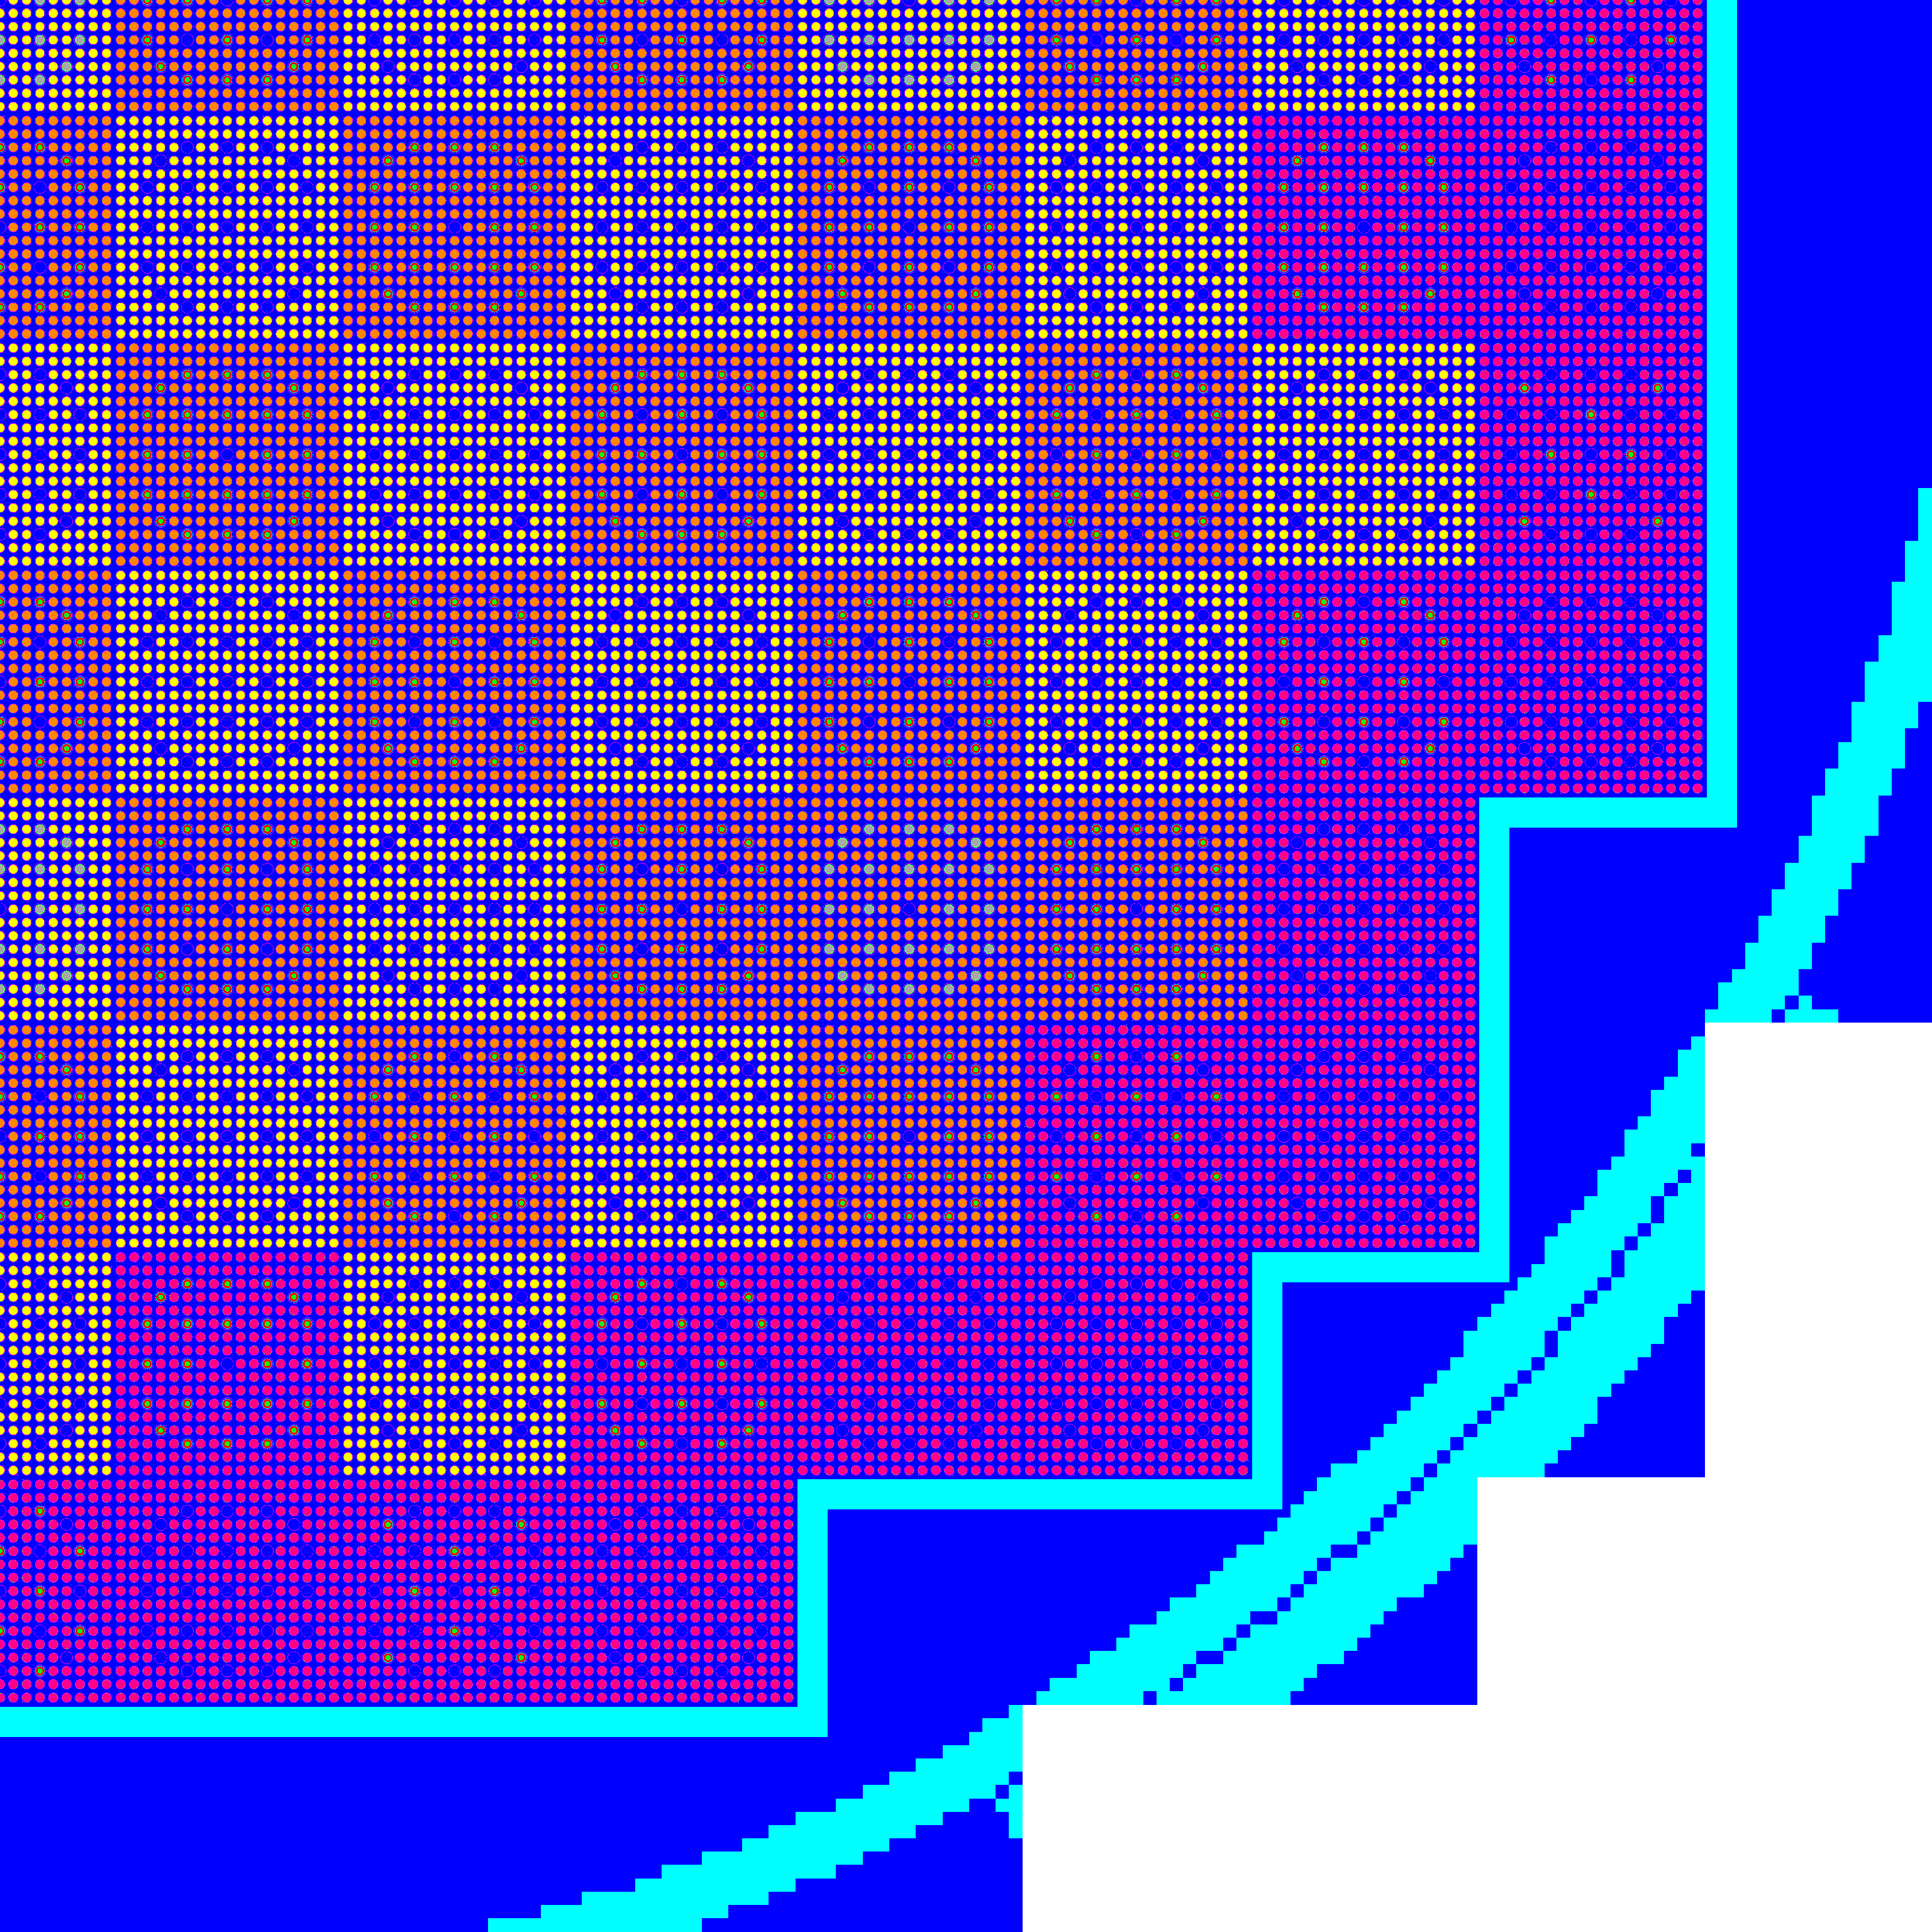
\includegraphics[width=0.9\textwidth]{5a-2d_core}
        \caption{fine mesh\label{fig:Spatial Decomposition:5a-2d configuration}}
      \end{subfigure}%
      ~
      \begin{subfigure}[t]{0.45\textwidth}
        \centering
        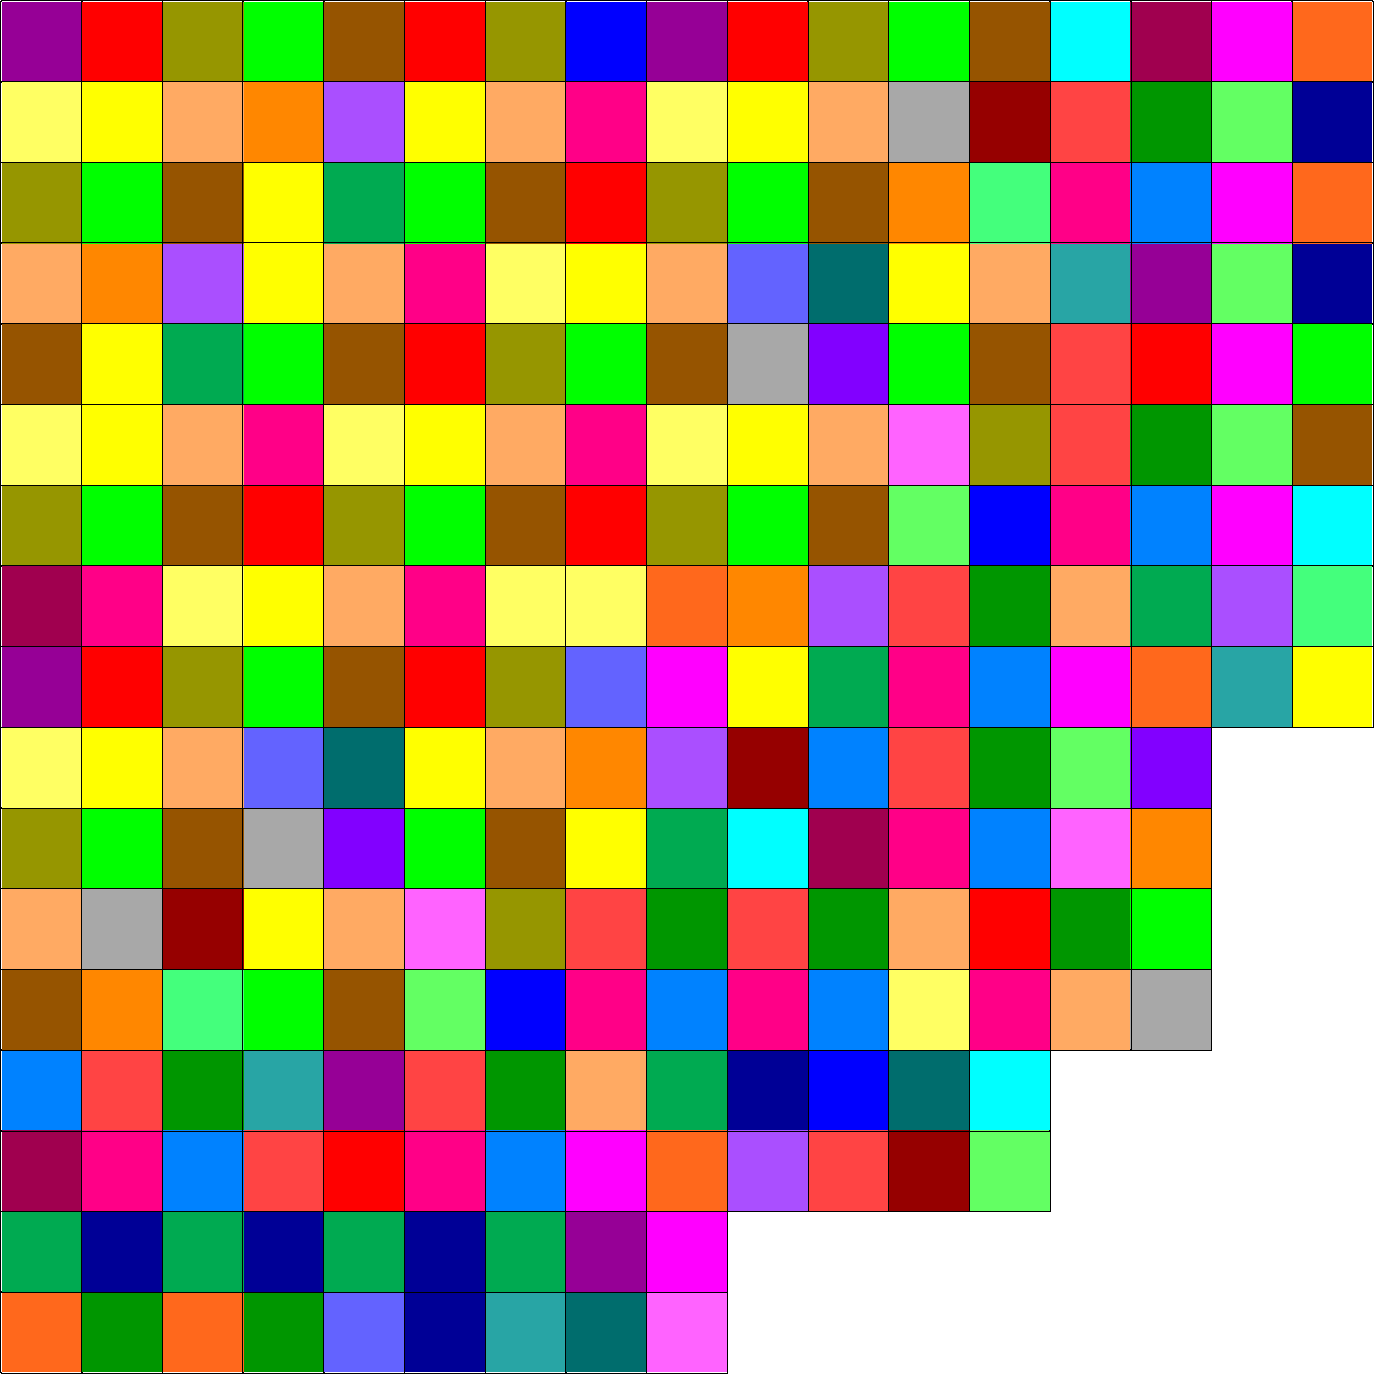
\includegraphics[width=0.9\textwidth]{modmesh_5a-2d}
        \caption{ray-tracing module mesh\label{fig:Spatial Decomposition:5a-2d modular mesh}}
      \end{subfigure}
      \caption{Example quarter core configuration and corresponding ray-tracing modular mesh in MPACT. \label{fig:Spatial Decomposition:5a-2d abstraction}}
    \end{figure}

    MPACT has had two spatial decomposition methods in the past: manual decomposition, and assembly-based decomposition.
    A user may manually enter a decomposition \cite{StimpsonPartitioning2017}, but it is time consuming to construct a balanced decomposition and will likely still be suboptimal to some degree.
    An automated method exists that recursively bisects the core using Morton-ordering \cite{Morton1966} applied to the reactor assembly geometries.
    While this method is automated, it often yields very imbalanced domains, and also restricts the number of subdomains that can be used.

    Previous work has shown that spatial decomposition of reactors can be abstracted to a graph partitioning problem \cite{Fitzgerald2017}.
    The use of graph partitioning methods in MPACT is expected to solve the issues encountered in each of the two approaches described above.
    These methods can be used to decompose into an arbitrary number of domains with high quality results, without user input.

    Existing graph partitioning libraries such as METIS \cite{METIS} partition graphs very efficiently and have very high quality results.
    To use all given processors, MPACT requires that each spatial subdomain contains at least one module, i.e. no partition can be empty.
    However, in some cases, particularly when the number of partitions is high, METIS may generate empty partitions.
    This means METIS cannot be used to decompose the core into an arbitrary number of subdomains without modifying the resulting partitions.
    For this reason, MPACT does not rely on third-party libraries for graph partitioning in the spatial decomposition process.
  }
  %%%%%%%%%%%%%%%%%%%%%%%%%%%%%%%%%%%%%%%%%%%%%%%%%%%%%%%%%%%%%%%%%%%%%%%%%%%%%%
  % Applied Graph Theory
  %%%%%%%%%%%%%%%%%%%%%%%%%%%%%%%%%%%%%%%%%%%%%%%%%%%%%%%%%%%%%%%%%%%%%%%%%%%%%%
  \section{Applied Graph Theory}{\label{sec:Spatial Decomposition:Applied Graph Theory}
    The spatial decomposition of a reactor core can be abstracted to the partitioning of a graph.
    Specifically, this would be a weighted graph, $G(V,E)$, that is comprised of a set of vertices, $V$, and a set of edges, $E$, that connect pairs of vertices.
    In general, these vertices and edges may have weights; a vertex $v_i$ will have weight $w_i$, and an edge $e_i$ between vertices $v_i$ and $v_j$ will have weight $c_{ij}$.
    In MPACT, a vertex represents a ray-tracing module, and the edges represent communication between adjacent modules in the \ac{MOC}.
    The graphs are undirected because communication between ray-tracing modules is two-way.

    Previous work \cite{Fitzgerald2017} applied unweighted graph partitioning techniques to the reactor spatial decomposition problem; the work presented here applies generalizations and improvements to the methods used for graphs with weighted vertices and edges.
    A vertex's weight indicates the amount of computational work that is needed; as one might expect, this is highly correlated with the number of computational cells.
    This is shown in \cref{sec:Spatial Decomposition:Results}.
    In general, the edges may also be weighted to account for different amounts of data transfer.
    This is discussed in more detail in \cref{sec:Spatial Decomposition:Applications for MPACT}.

    The goal of partitioning is for each subdomain to have equal weight, with minimal weight of edges cut by partition boundaries.
    This is equivalent to each subdomain having the same amount of computational work with minimized communication between processes.
    If each process has roughly the same amount of work to perform, then less time will be spent waiting for other processes, thus improving parallel efficiency.
    Also, with less communication, less time will be spent passing data between processes, so the parallel overhead will be reduced.

    In this work, methods were separated into two distinct categories: partitioning methods and partition refinement (improvement) methods.
    Partitioning methods give a near-balanced partitioning for a given graph.
    Refinement methods attempt to reduce communication between existing partitions in a graph.
    As applied in MPACT, these refinement methods typically did not significantly reduce communication.
    These methods and results are presented in \cref{sec:Spatial Decomposition:Partition Refinement}.
    %%%%%%%%%%%%%%%%%%%%%%%%%%%%%%%%%%%%%%%%%%%%%%%%%%%%%%%%%%%%%%%%%%%%%%%%%%%%
    % Graph Partitioning Methods
    %%%%%%%%%%%%%%%%%%%%%%%%%%%%%%%%%%%%%%%%%%%%%%%%%%%%%%%%%%%%%%%%%%%%%%%%%%%%
    \subsection{Graph Partitioning Methods}{\label{ssec:Spatial Decomposition:Graph Partitioning Methods}
      In this work, recursive partition methods were considered due to their capability to partition into arbitrary numbers of domains.
      Each of these recursive partitioning methods sorts the graph, using different methods, and then divides or ``cuts'' the graph into two sub-graphs with approximately equal vertex weights.
      Once a graph's vertices are sorted into a list, $V_s$, the graph can be bisected using \cref{alg:Graph Cutting}.

      Multi-level partitioning methods are widely used in other fields such as networking, where graphs can become very large; however, in MPACT, the number of ray-tracing modules is on the order of a few hundred to several thousand, which directly correlates to the size of the graph.
      Additionally, for MPACT, the decomposition problem is static, so the computation time for partitioning is expected to be negligible as it can simply be performed one time at the outset.
      Due to the small graph size, multi-level methods were not considered as part of this work.

      \begin{algorithm}[ht]
        \centering
        \caption{The algorithm used to determine how to cut a graph, $G(V,E)$, into two sub-graphs based on a sorted vertex list $V_s$, and that the graph will be recursively partitioned into $N$ groups.}
        \label{alg:Graph Cutting}
        \begin{algorithmic}[1]
          \Procedure{Graph Cut}{$G(V,E), V_s, N$}
            \State{$N_1 \gets \floor{N/2}$} \Comment{Desired number of recursive partitions for first subgraph}
            \State{$W_1 \gets \frac{N_1}{N}\suml[v_i\in V]w_i$} \Comment{Ideal weight of first subgraph}
            \State{Let $V_1$ be a set of vertices such that:
                \begin{itemize}[leftmargin=1.5cm]
                    \item{$V_1 \subset V$}
                    \item{The vertices $V_1$ are taken in order from $V_s$}
                    \item{$W_1 - \suml[v_i\in V_1] w_i$ is minimized}
                \end{itemize}
            }
            \State{Let $V_2$ be the subset $V \setminus V_1$}
            \State{Optionally call a refinement method}
            \State{Create a graph $G_1$ from $V_1$}
            \State{Create a graph $G_2$ from $V_2$}
          \EndProcedure
        \end{algorithmic}
      \end{algorithm}
      %%%%%%%%%%%%%%%%%%%%%%%%%%%%%%%%%%%%%%%%%%%%%%%%%%%%%%%%%%%%%%%%%%%%%%%%%%
      % Recursive Spectral Bisection
      %%%%%%%%%%%%%%%%%%%%%%%%%%%%%%%%%%%%%%%%%%%%%%%%%%%%%%%%%%%%%%%%%%%%%%%%%%
      \subsubsection{Recursive Spectral Bisection}{\label{sssec:Spatial Decomposition:Recursive Spectral Bisection}
        The \ac{RSB} method, originally developed by \citet{Pothen1989}, has been highly successful and widely used in graph partitioning \cite{Simon1991,Spielman2007}.
        This method relies entirely on the connectivity of the graph and not on its geometry.
        The \ac{RSB} method has been improved to allow for partitioning of \emph{weighted} graphs into any number of domains \cite{Hsieh1995}.

        The \ac{RSB} method makes use of the Laplacian matrix of a graph; specifically the second-smallest eigenvalue of this matrix, referred to by Fiedler as the \emph{algebraic connectivity} \cite{Fiedler1973}.
        The eigenvector associated with this eigenvalue has also been known as the \emph{Fiedler vector}.
        For weighted graphs, the weighted Laplacian matrix is used in lieu of the Laplacian matrix; matrix elements are given by
        \begin{align}
          \label{eq:Spatial Decomposition:Weighted Laplacian}
          L_{ij} =
            \begin{cases}
              d_i, \quad&{i=j},\\
              -c_{ij}, \quad&{i\neq j},\\
              0, \quad&{\text{else}},
            \end{cases}
        \end{align}
        where $d_i$ is the sum of edge weights from vertex $v_i$, and $c_{ij}$ is the weight of the edge between vertices $v_i$ and $v_j$.
        The Fiedler vector is found from this weighted Laplacian matrix; by sorting the values of the Fiedler vector, the vertices can be reordered in a one-dimensional list $V_s$.
        This list of vertices is then divided into two sets, based on weight and total number of partitions needed (see \cref{alg:Graph Cutting}).
        The recursive spectral bisection algorithm is listed in \cref{alg:Recursive Spectral Bisection}.

        \begin{algorithm}
          \centering
          \caption{The recursive spectral bisection (RSB) algorithm.}
          \label{alg:Recursive Spectral Bisection}
          \begin{algorithmic}[1]
            \Procedure{RSB}{$G(V,E)$}
              \State{Let $L$ be the weighted Laplacian of $G(V,E)$}
              \State{Compute eigenvectors of $L$}
              \State{Use the Fiedler vector to sort $V\to V_s$} \Comment{If tie, use larger eigenvectors}
              \State{Cut graph into $G_1(V_1,E_1), G_2(V_2,E_2)$: \Cref{alg:Graph Cutting}}
              \State{RSB($G_1(V_1,E_1)$)}
              \State{RSB($G_2(V_2,E_2)$)}
            \EndProcedure
          \end{algorithmic}
        \end{algorithm}
      }
      %%%%%%%%%%%%%%%%%%%%%%%%%%%%%%%%%%%%%%%%%%%%%%%%%%%%%%%%%%%%%%%%%%%%%%%%%%
      % Recursive Inertial Bisection
      %%%%%%%%%%%%%%%%%%%%%%%%%%%%%%%%%%%%%%%%%%%%%%%%%%%%%%%%%%%%%%%%%%%%%%%%%%
      \subsubsection{Recursive Inertial Bisection}{\label{sssec:Spatial Decomposition:Recursive Inertial Bisection}
        Another class of recursive partitioning methods are coordinate or geometric methods.
        There are many different geometric partitioning methods in existence; in this study, the \ac{RIB} method \cite{Elsner1997,Floros1995} was investigated.
        This method uses only the geometry of the graph to construct a bisector and does not consider the connectivity (edges) in any way.

        The \ac{RIB} method determines a bisector which cuts the graph into two approximately equally sized subdomains.
        This is easily generalized for weighted graphs.
        The bisector should have approximately equal amounts of weight on each side.
        The \ac{RIB} makes no assumption of the orientation of the graph in space, unlike some other coordinate partitioning methods.
        The principle axes of the graph are equivalent to the eigenvectors of the inertial matrix given by
        \begin{equation}
          \label{eq:Spatial Decomposition:Inertial Matrix}
          \mat{I} \defined \suml[i=1][n] w_i\left(\vec{x}_i-\avg{\vec{x}}\right)^T\left(\vec{x}_i-\avg{\vec{x}}\right),
        \end{equation}
        where $n$ is the number of vertices, $\vec{x}_i$ is a row-vector containing coordinates of vertex $v_i$, and $\avg{\vec{x}}$ is the mean coordinate vector given by
        \begin{equation}
          \label{eq:Spatial Decomposition:Mean Coordinates}
          \avg{\vec{x}} \defined \frac{\suml[i=1][n] w_i \vec{x_i}}{\suml[i=1][n] w_i}.
        \end{equation}
        An approximate bisector is given as passing through the weighted centroid with normal vector given as one of the eigenvectors of $\mat{I}$.

        Other works \cite{Elsner1997,Floros1995} have used the smallest eigenvalue's eigenvector as a normal vector to minimize the mean-square distance of vertices from the bisecting line or plane.
        However, in this work, the largest eigenvalue's eigenvector is used, so a smaller cut-size is typically given while still bisecting the graph into two subdomains of approximately equal weight.
        This is the case because in the \ac{MOC}, communication scales with the surface area between adjacent ray-tracing modules.
        This may not be the case for other computational methods.

        In general, a line or plane passing through the weighted centroid with the eigenvector normals will not cut the graph into two equally weighted subdomains.
        Instead, the vertices will be sorted according to their distance from the approximate bisectors, and then a cut will be made so that near equal amounts of weight are in each set using \cref{alg:Graph Cutting}.
        This sorting and cutting based on weights is equivalent to shifting the bisector in the direction of the normal vector.
        An example is visualized in \cref{fig:Spatial Decomposition:RIB Diagram}.
        The \ac{RIB} algorithm is listed in \cref{alg:Recursive Inertial Bisection}.

        \begin{algorithm}
          \centering
          \caption{The basic \acf{RIB} algorithm.}
          \label{alg:Recursive Inertial Bisection}
          \begin{algorithmic}[1]
            \Procedure{RIB}{$G(V,E)$}
              \State{Compute the weighted centroid of the graph $\avg{\vec{x}}$, given by \cref{eq:Spatial Decomposition:Mean Coordinates}}
              \State{Shift coordinates relative to centroid: $\vec{x}^c_i = \vec{x}_i - \avg{\vec{x}} \quad{\forall i\in V}$}
              \State{Compute inertial matrix $\mat{I}$, given by \cref{eq:Spatial Decomposition:Inertial Matrix}}
              \State{Compute eigenvectors of $\mat{I}$. Largest eigenvalue's eigenvector $\vec{e}_1$}
              \State{Compute distance from largest eigen-pair bisector: $d_i = \vec{x}^c_i \cdot \vec{e}_1$}
              \State{Sort $V \to V_s$ based on $d_i$.} \Comment{In ties use smaller eigenvalue's eigenvector}
              \State{Cut graph into $G_1(V_1,E_1), G_2(V_2,E_2)$: \Cref{alg:Graph Cutting}}
              \State{RIB($G_1(V_1,E_1)$)}
              \State{RIB($G_2(V_2,E_2)$)}
            \EndProcedure
          \end{algorithmic}
        \end{algorithm}

        \begin{figure}
          \centering
          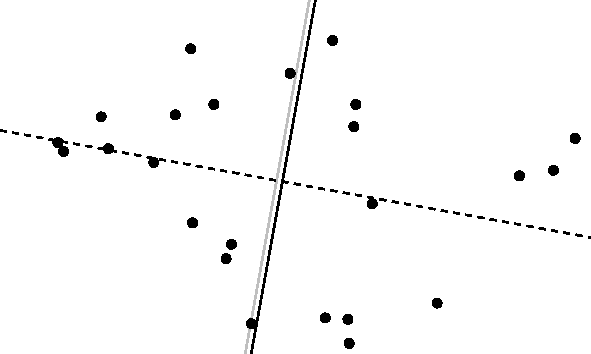
\includegraphics[width=0.85\linewidth]{RIB/RIB_diagram}
          \caption{
            Example of an inertial bisection.
            Vertices are shown as black points, the bisectors of the largest eigen-pair is shown by the black solid, and the bisector of the smallest eigen-pair is shown by the black dashed line.
            The ``shifted'' bisector used in the partitioning is shown in grey.
            While the communication between vertices is not drawn, it is clear that the length (proportional to cut size) of the smallest eigen-pair bisector is larger than that of the largest eigen-pair bisector.
            \label{fig:Spatial Decomposition:RIB Diagram}
          }
        \end{figure}
      }
      %%%%%%%%%%%%%%%%%%%%%%%%%%%%%%%%%%%%%%%%%%%%%%%%%%%%%%%%%%%%%%%%%%%%%%%%%%
      % Recursive Expansion-Based Methods
      %%%%%%%%%%%%%%%%%%%%%%%%%%%%%%%%%%%%%%%%%%%%%%%%%%%%%%%%%%%%%%%%%%%%%%%%%%
      \subsubsection{Recursive Expansion-Based Methods}{\label{sssec:Spatial Decomposition:Recursive Expansion-Based Methods}
        The \ac{REB} methods comprise the last class of partitioning methods examined in this work.
        These methods begin a bisection step by selecting a vertex as the starting point of a subdomain.
        This subdomain is then expanded until it is approximately half the size of the graph \cite{Farhat1988,Nasra1991,Elsner1997,Fitzgerald2017}.
        In this work, the method outlined by \citet{Fitzgerald2017} was slightly modified and generalized to weighted graphs.
        For the remainder of this work, the acronym \emph{\ac{REB}} will be used to denote this specific expansion-based method rather than the entire class of methods.

        This \ac{REB} method considers both the geometry and connectivity of the graph.
        The method begins by choosing a starting vertex for the subdomain and then expands based on a set of prioritized rules.
        At each expansion step, the next vertex is chosen so that it is geometrically close to the vertices within the subdomain and to minimize edges between the subdomain and the remaining graph.
        However, this method makes the assumptions that the mesh is structured, and that every mesh element is the same shape and size.
        For the application in MPACT, this is always true.

        This \ac{REB} method uses the concept of a \emph{\ac{SOI}} around a vertex.
        The \ac{SOI} includes directly neighboring vertices and vertices that neighbor more than one of the direct neighbors or that would if the direct neighbor were present in each structured position around the primary vertex.
        This is shown for 2-D rectangular structured mesh in \cref{fig:Spatial Decomposition:Sphere of Influence}.
        In the implementation, the sphere of influence is calculated using a geometric distance rather than connectivity.

        The starting vertex in this \ac{REB} method is chosen using a set of prioritized rules:
        \begin{enumerate}
            \item{must be on graph boundary, i.e. at least one direct neighbor is not present,}
            \item{must have the lowest summed weight of edges, and}
            \item{must be located furthest from weighted centroid (given by \cref{eq:Spatial Decomposition:Mean Coordinates}).}
        \end{enumerate}
        These rules prioritize the domain beginning its' expansion in a ``corner'' of the graph; this helps to avoid the creation of disjoint subdomains.
        Vertices within the expanding subdomain are considered internal vertices, and the remaining vertices are considered to be external vertices.
        During expansion, the next vertex is determined using a set of prioritized rules:
        \begin{enumerate}
            \item{must be neighboring at least one internal vertex,}
            \item{must have the highest summed weight of edges with internal vertices,}
            \item{must have the lowest summed weight of edges with external vertices,}
            \item{must have the largest number of internal SOI vertices,}
            \item{must have the largest number of external SOI vertices, and}
            \item{must have the smallest distance from reference vertex.}
        \end{enumerate}
        The reference vertex is in the expanding subdomain, which begins as the first vertex but changes during expansion; the reference vertex is the most recently added vertex with less external communication than the previously added vertex.
        An example of the expansion order is shown in \cref{fig:Spatial Decomposition:REB Expansion Order}.
        The rules ensure that the next vertex is connected to the current domain, and prioritizes minimizing communication, and avoids creating disjoint subdomains.

        \begin{algorithm}
          \centering
          \caption{The chosen Recursive Expansion Bisection (REB) algorithm.}
          \label{alg:Recursive Expansion Bisection}
          \begin{algorithmic}[1]
            \Procedure{REB}{$G(V,E)$}
              \State{Compute weighted centroid of the graph}
              \State{Choose a starting vertex for the expanding domain: See rules in \cref{sssec:Spatial Decomposition:Recursive Expansion-Based Methods}}
              \State{Expand the domain from the starting vertex. Let $V_s$ be the list of vertices in order of the expansion: See rules in \cref{sssec:Spatial Decomposition:Recursive Expansion-Based Methods}}
              \State{Cut graph into $G_1(V_1,E_1), G_2(V_2,E_2)$: \Cref{alg:Graph Cutting}}
              \State{REB($G_1(V_1,E_1)$)}
              \State{REB($G_2(V_2,E_2)$)}
            \EndProcedure
          \end{algorithmic}
        \end{algorithm}

        \begin{figure}
          \centering
          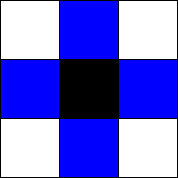
\includegraphics[width=0.45\linewidth]{REB/SoI_Rectangular}
          \caption{
              ``Sphere of influence'' example for 2-D rectangular structured grid.
              The primary vertex is shown in black, direct neighbors are blue, and additional vertices in the sphere are white.
              \label{fig:Spatial Decomposition:Sphere of Influence}
          }
        \end{figure}

        \begin{figure}
          \centering
          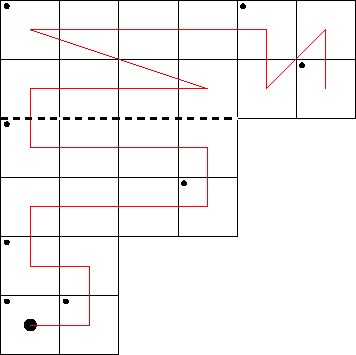
\includegraphics[width=0.65\linewidth]{REB/Expansion}
          \caption{
              An example of the \ac{REB} method expansion on a small graph.
              The black lines show the square mesh cells.
              The expansion begins at the large black point in the center of a cell, and the red line from this shows the expansion's order.
              Each small black dot in the upper left of a cell indicates the reference vertices during expansion.
              The thick black dashed line shows the bisecting cut.
              \label{fig:Spatial Decomposition:REB Expansion Order}
          }
        \end{figure}

      }
    }
  }
  %%%%%%%%%%%%%%%%%%%%%%%%%%%%%%%%%%%%%%%%%%%%%%%%%%%%%%%%%%%%%%%%%%%%%%%%%%%%%%
  % Applications for MPACT
  %%%%%%%%%%%%%%%%%%%%%%%%%%%%%%%%%%%%%%%%%%%%%%%%%%%%%%%%%%%%%%%%%%%%%%%%%%%%%%
  \section{Applications for MPACT}{\label{sec:Spatial Decomposition:Applications for MPACT}
    As described in \cref{sec:Spatial Decomposition:Spatial Decomposition in MPACT}, MPACT's spatial decomposition is performed on the ray-tracing module mesh.
    However, there are a couple of restrictions on spatial subdomains in MPACT.
    Each spatial subdomain must be contiguous, and cannot wrap around other spatial subdomains.
    To account for these restrictions, adaptations are made to the graph partitioning process.

    Due to restrictions in MPACT, at each recursive step, each subdomain in a bisection is made contiguous.
    If a partitioning method results in a noncontiguous subdomain, then each noncontiguous group of modules will be moved into the other subdomain except for the largest group.
    This fix is done at the expense of load-balance, but is necessary for these methods to be robust in MPACT.
    To ensure that no subdomain wraps around another, a fix is applied after the graph partitioning process.
    If a subdomain wraps around another, then the concave subdomain will be given the modules it wraps around.

    The ray-tracing modules that make up the core in MPACT can be abstracted into a weighted graph, where vertex weights are the number of computational cells in a module, and edges connecting neighboring modules.
    These edges represent the communication in MPACT's \ac{MOC} solver.
    However, MPACT typically relies on the \ac{CMFD} acceleration method \cite{Smith1983}, which involves solving a sparse linear system.
    The work-load and communication of the \ac{CMFD} solver, in MPACT this is a linear system solver from PETSc \cite{Petsc}, are different than than of the \ac{MOC}.
    Thus, what may be an optimal decomposition for the \ac{MOC} solver, is likely not for the \ac{CMFD} solver.
    As the \ac{MOC} solver is expected to take longer than the \ac{CMFD} solver, the graph is constructed based on the work-load and communication of \ac{MOC}.

    For 2-D simulations, the application of graph partitioning methods is clear: abstract the 2-D mesh into a graph for partitioning.
    However, for 3-D, there are additional concerns.
    MPACT's primary 3-D transport method is the 2D-1D method, in which the \ac{MOC} is used in the radial directions, and a lower-order solver couples axial planes \cite{Collins2016}.
    For 2D-1D simulations, MPACT currently restricts spatial domains to be aligned in both the radial and axial directions; this is due to implementation, and is not a general requirement of the methods.

    To comply with MPACT's restrictions on 3-D spatial domains, the current approach is to axially average module weights (numbers of cells), perform a 2-D graph partitioning on a single plane, and apply the resulting partitioning to all axial planes.
    This approach will restrict the number of spatial domains to be an integer multiple of the number of planes.
    This axially and radially aligned scheme is expected to work well in many cases since reactor cores do not typically vary significantly in the axial direction.
    However, for some designs, this may not be true, and planes near the top or bottom of the core have significantly fewer cells; in these cases, high load imbalance is to be expected.

    It is possible to change MPACT's implementation to lift these alignment restrictions, but that is beyond the scope of this work.
    If spatial domains were aligned in only the radial direction, there may be some benefit to load-balance.
    In this scheme, each axial plane can be assigned an appropriate number of processes, and a separate 2-D decomposition can be performed for each plane.
    This also lifts restrictions on the number of domains; the number of domains must only be greater than or equal to the number of planes.

    If all alignment restrictions were lifted on MPACT's spatial domains, then a direct partitioning of the 3-D core can be performed by abstracting the entire core to a graph.
    This scheme provides the most freedom and would be expected to give the most balanced decompositions.
    In MPACT's 2D-1D solver, the amount of data communicated radially is significantly larger than that communicated axially, so it may be advantageous to assign the edges connecting the neighboring modules in the axial direction lower weights than those in radial directions.
    By doing so, the overall communication would be expected to be decreased.

    \begin{figure}
      \centering
      \begin{subfigure}[t]{0.3\textwidth}
        \centering
        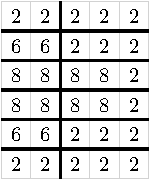
\includegraphics[width=0.9\textwidth]{alignmentComparison/pac_axial}
        \caption{}
      \end{subfigure}%
      ~
      \begin{subfigure}[t]{0.3\textwidth}
        \centering
        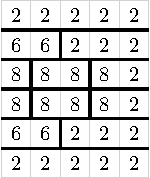
\includegraphics[width=0.9\textwidth]{alignmentComparison/pac_radial}
        \caption{}
      \end{subfigure}%
      ~
      \begin{subfigure}[t]{0.3\textwidth}
        \centering
        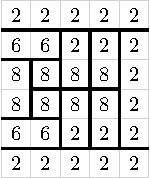
\includegraphics[width=0.9\textwidth]{alignmentComparison/pac_general}
        \caption{}
      \end{subfigure}
      \caption{
        Sample decompositions for (a) axially aligned, (b) radially aligned, and (c) generalized decomposition strategies.
        Rows represent axial planes.
        Numbers are the vertex weights.
        \label{fig:Spatial Decomposition:partitionAlignmentComparison}
      }
    \end{figure}

    \Cref{fig:Spatial Decomposition:partitionAlignmentComparison} shows a comparison of the three hypothetical decomposition schemes, for the purposes of illustration.
    Looking at the \ac{MMR}, as an indicator of load-balance, the strategies have clear differences.
    The \ac{MMR} for the axially aligned, radially aligned, and generalized strategies in this example are $4.00$, $2.67$, and $2.00$, respectively.
    However, it is important to note that the largest domain in each case has the same weight (16), so while the different schemes give different balances, the overall run-times are not expected to be different.
  }
  %%%%%%%%%%%%%%%%%%%%%%%%%%%%%%%%%%%%%%%%%%%%%%%%%%%%%%%%%%%%%%%%%%%%%%%%%%%%%%
  % Results
  %%%%%%%%%%%%%%%%%%%%%%%%%%%%%%%%%%%%%%%%%%%%%%%%%%%%%%%%%%%%%%%%%%%%%%%%%%%%%%
  \section{Results}{\label{sec:Spatial Decomposition:Results}
    %%%%%%%%%%%%%%%%%%%%%%%%%%%%%%%%%%%%%%%%%%%%%%%%%%%%%%%%%%%%%%%%%%%%%%%%%%%%
    % 2-D Results
    %%%%%%%%%%%%%%%%%%%%%%%%%%%%%%%%%%%%%%%%%%%%%%%%%%%%%%%%%%%%%%%%%%%%%%%%%%%%
    \subsection{2-D Results}{\label{ssec:Spatial Decomposition:2-D Results}
      Results were generated for the planar 2-D version of VERA progression problem 5a \cite{VERAProblems}.
      This problem is a quarter core with reflector, barrel, and neutron pad regions surrounding several fuel assemblies, as shown in \cref{fig:Spatial Decomposition:5a-2d}.
      In the model, there are 257 ray-tracing modules in total, which provides the upper bound for the number of domains.
      Each subdomain is assigned to a single processor, with a maximum of 36 processors (subdomains) per computational node.
      Each of the graph decomposition methods was applied to the geometry of this problem, and MPACT was run for each case without applying refinement methods.
      The assembly-based decomposition was run for all possible numbers of subdomains: 1, 4, 16, 73, and 257.
      The possible numbers of subdomains are limited by powers of 4 (8 in 3-D), until subdomains would be located entirely outside the core shape.
      It is also possible to decompose into the fuel assemblies or ray-tracing modules, in this case 73 and 257 respectively.
      Example decompositions for 73 subdomains are shown in \cref{fig:Spatial Decomposition:5a-2d example decomp}.

      \begin{figure}
        \centering
        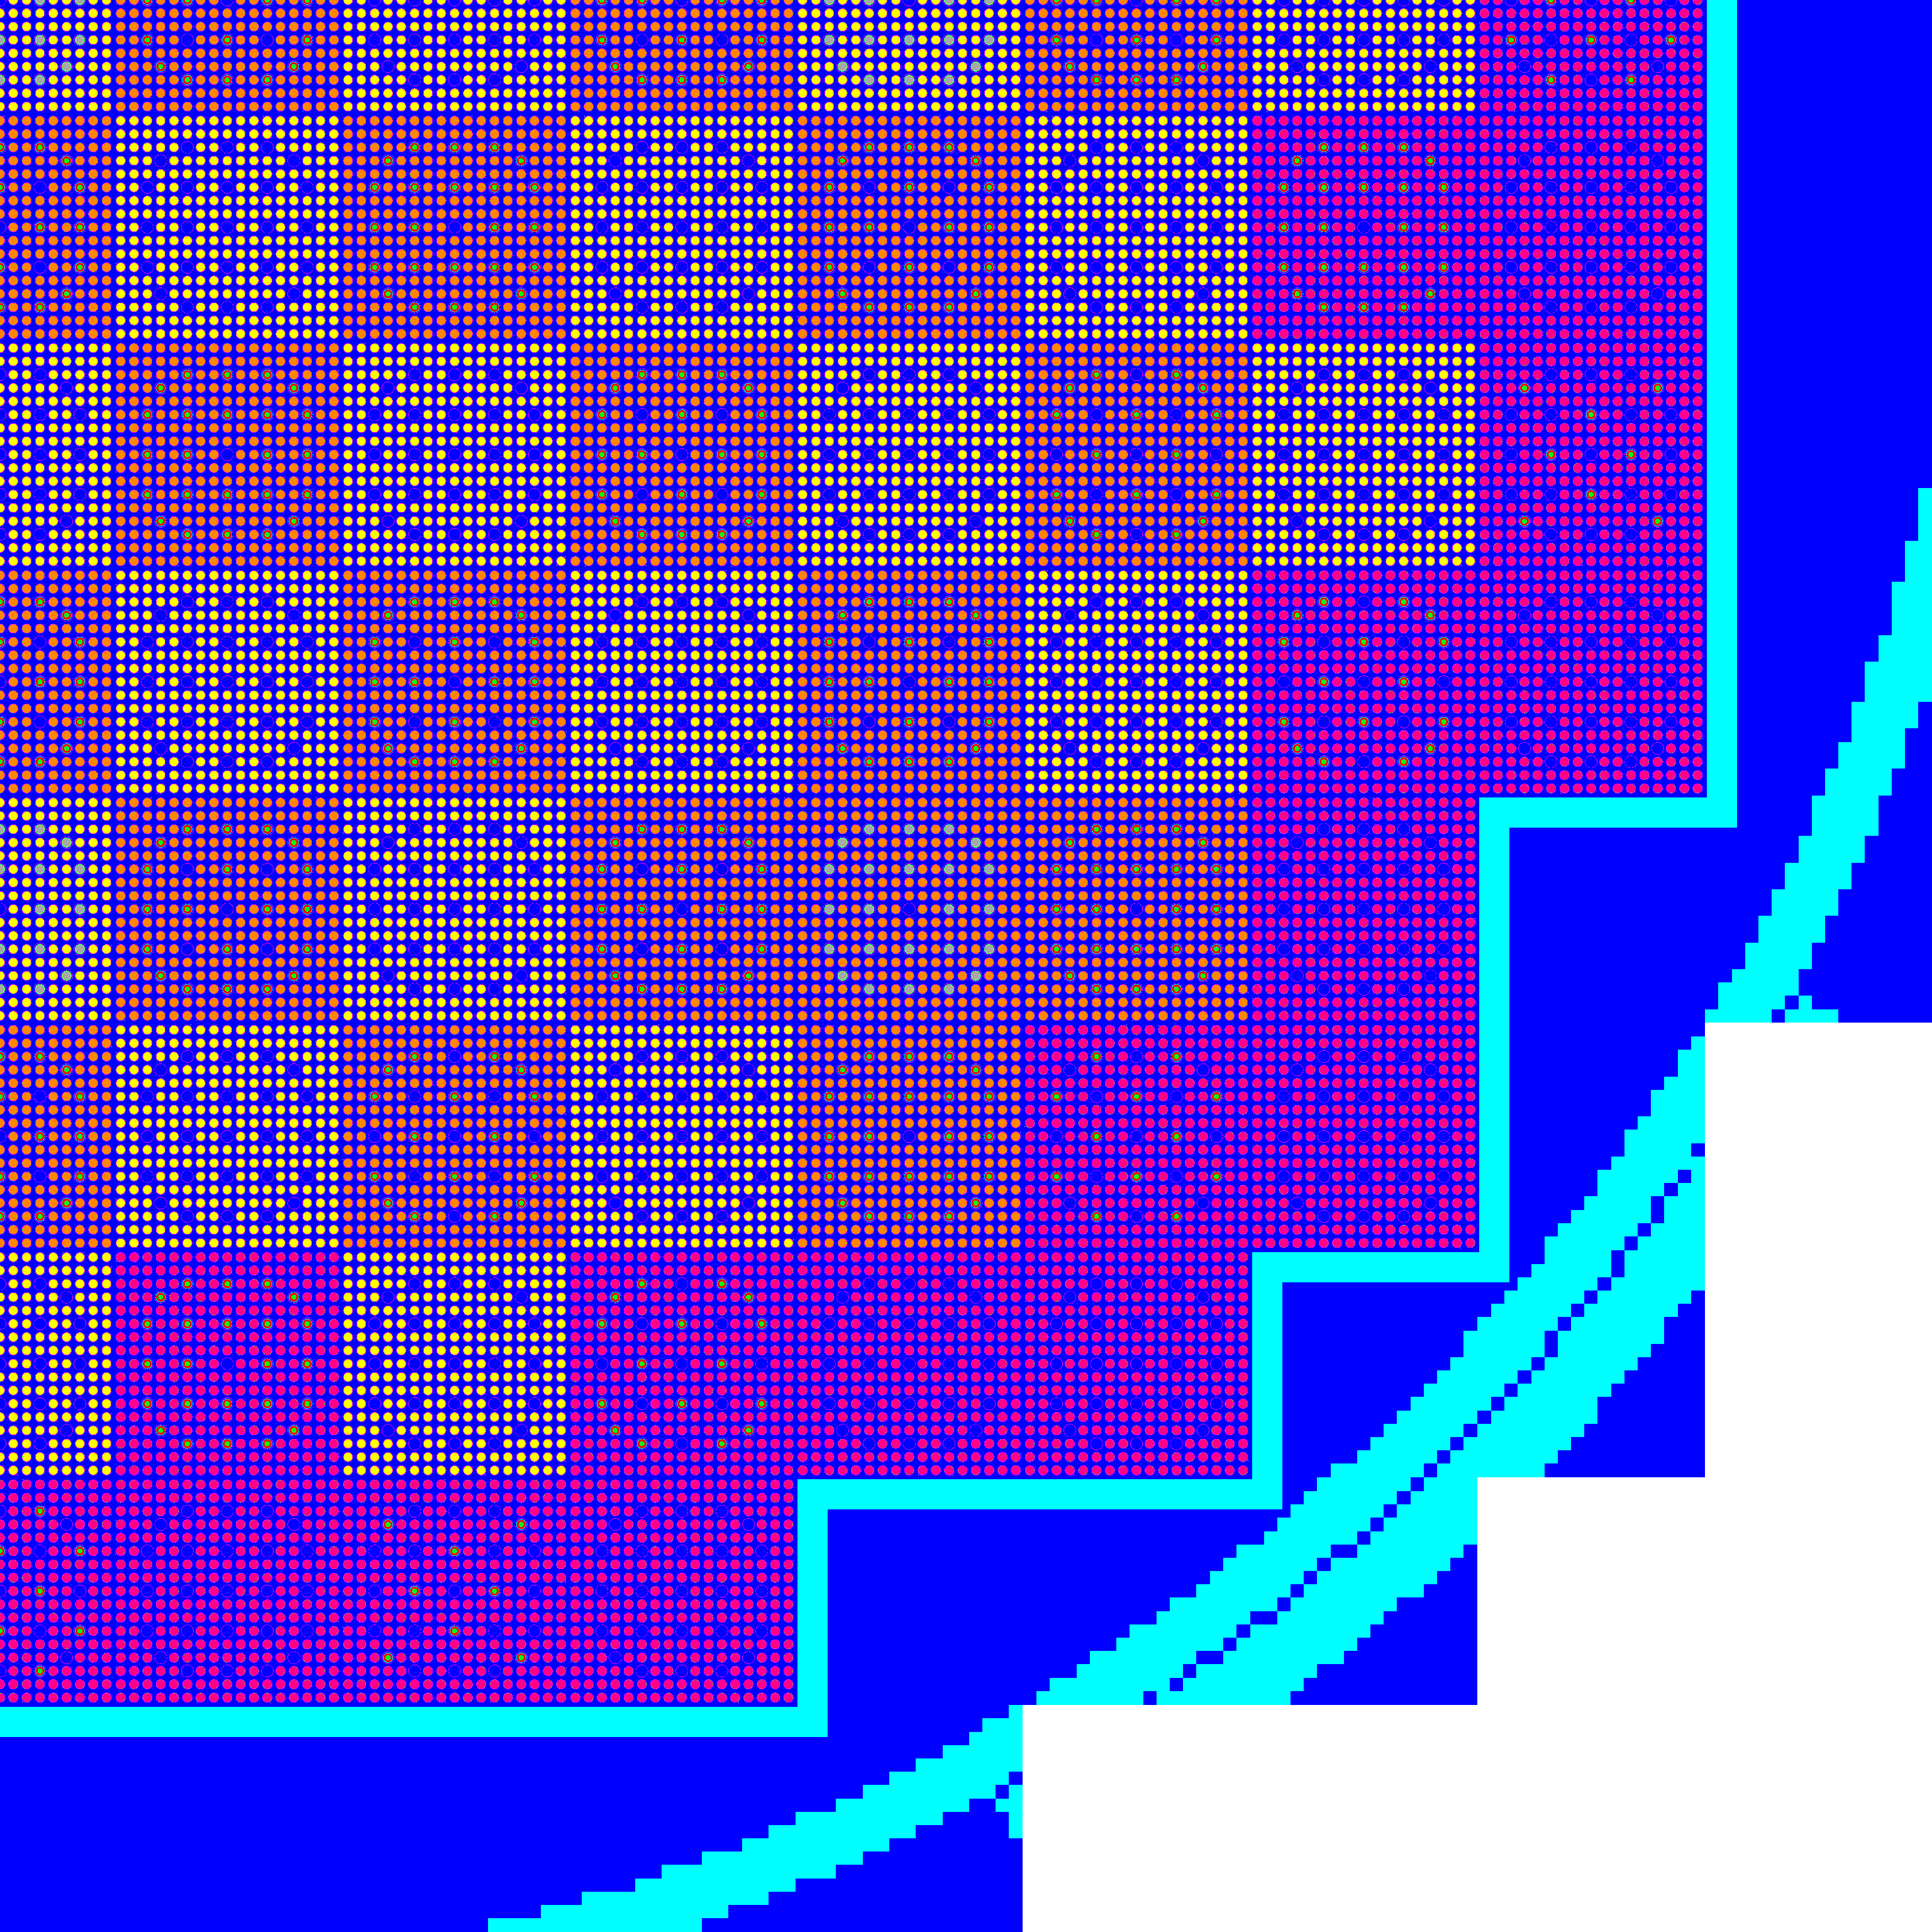
\includegraphics[width=0.35\textwidth]{5a-2d_core}
        \caption{VERA progression problem 5a-2d core configuration. \label{fig:Spatial Decomposition:5a-2d}}
      \end{figure}

      \begin{figure}[H]
        \centering
        \begin{subfigure}[t]{0.45\textwidth}
          \centering
          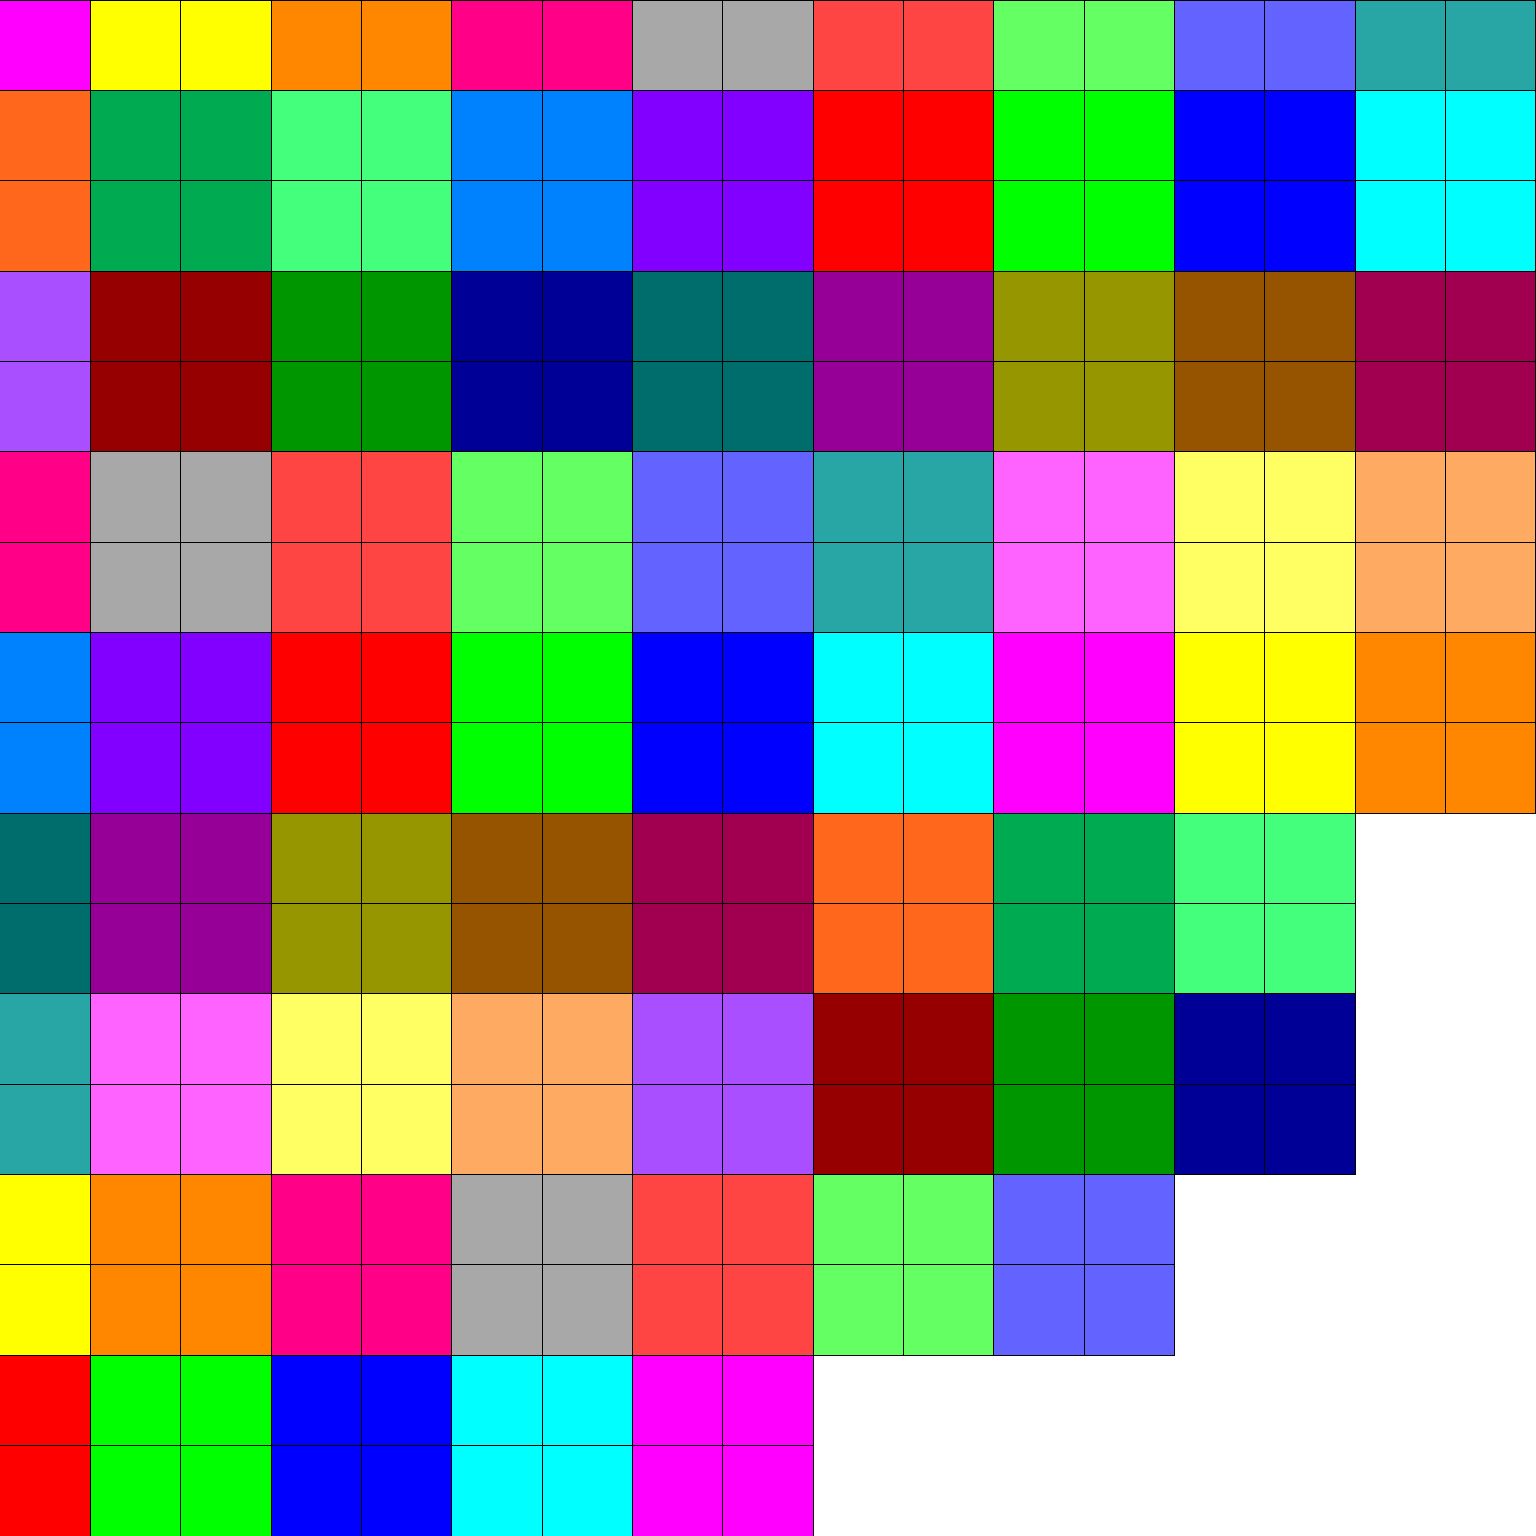
\includegraphics[width=0.9\textwidth]{results/2D/Assembly}
          \caption{Assembly-based decomposition method. \label{fig:Spatial Decomposition:5a-2d 73 Assembly}}
        \end{subfigure}%
        ~
        \begin{subfigure}[t]{0.45\textwidth}
          \centering
          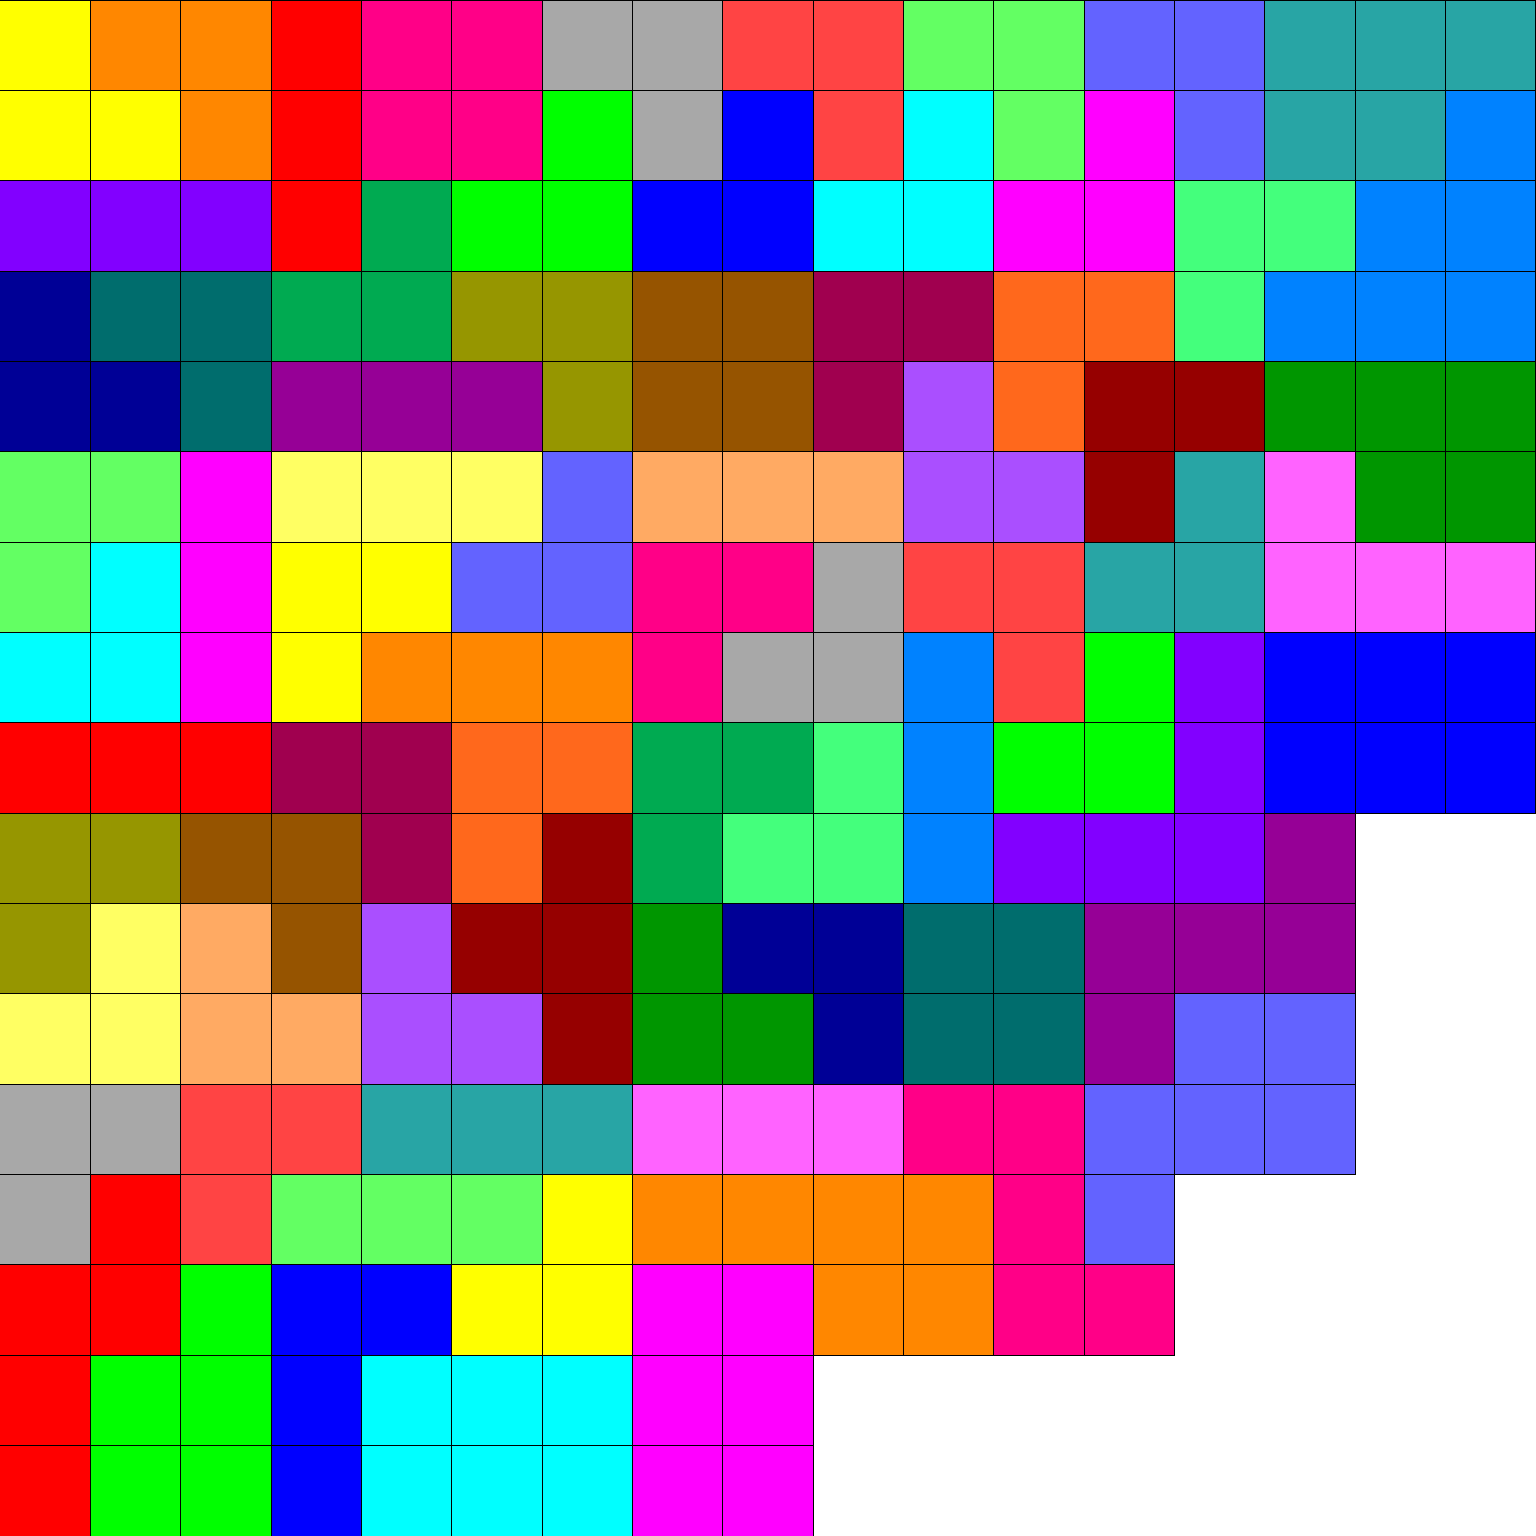
\includegraphics[width=0.9\textwidth]{results/2D/REB_none}
          \caption{\ac{REB} partitioning method. \label{fig:Spatial Decomposition:5a-2d 73 REB None}}
        \end{subfigure}
        \caption{
          Example decompositions for 73 subdomains for VERA progression problem 5a-2d.
          Each color represents a different subdomain.
          \label{fig:Spatial Decomposition:5a-2d example decomp}
        }
      \end{figure}

      %%%%%%%%%%%%%%%%%%%%%%%%%%%%%%%%%%%%%%%%%%%%%%%%%%%%%%%%%%%%%%%%%%%%%%%%%%
      % Load-Balance
      %%%%%%%%%%%%%%%%%%%%%%%%%%%%%%%%%%%%%%%%%%%%%%%%%%%%%%%%%%%%%%%%%%%%%%%%%%
      \subsubsection{Load-Balance}{\label{sssec:Spatial Decomposition:Load-Balance}
        In MPACT, each spatial subdomain is simulated concurrently.
        After each iteration, parallel boundary conditions are communicated and updated in parallel.
        The time for solve routines is measured for each subdomain, as is the \ac{MOC} communication time.
        However, the communication time includes time spent waiting for other subdomains to finish computation; that is, blocking communication.

        This parallel iteration scheme means that the wall-time of each iteration is controlled by the subdomain with the longest run-time; this is expected to be the subdomain with the largest number of cells.
        However, the wall-time is not the only important consideration; it is important to consider how well the computational resources are used.
        A measure for how well computational resources are used is the parallel efficiency, as defined by
        \begin{equation}
            \label{eq:Spatial Decomposition:Parallel Efficiency}
            E \defined \frac{T_s}{N \cdot T},
        \end{equation}
        where $T_s$ is the time in serial, and $T$ is the time in parallel with $N$ processes.

        If runtime is highly correlated with the largest number of cells in a subdomain, then this efficiency is expected to be related to the largest \emph{fraction} of cells in a subdomain.
        Specifically, the parallel efficiency is expected to be inversely proportional to the ratio of the largest fraction of cells to the optimal fraction of cells.
        In an ideally balanced decomposition, each subdomain would have $1/N$ cell fraction.
        By comparing the maximum cell fraction to this optimal value, one can estimate how much longer the simulation will take compared to an ideal decomposition, neglecting serial code sections and overhead.

        Higher parallel efficiency indicates better utilization of the available computational resources, and lower runtime.
        The expectation is that higher parallel efficiency can be obtained by having the largest cell fraction closer to the optimal cell fraction.
        As seen in \cref{fig:Spatial Decomposition:Max/Optimal Ratio}, the \ac{REB} method is expected to have slightly better parallel efficiency than the other methods for many cases.
        It is also expected that for a low number of subdomains, the assembly-based decomposition will result in significantly lower parallel efficiency.
        However, for large numbers of subdomains, the assembly-based decomposition is expected to result in comparable parallel efficiency to the graph partitioning methods.

        \begin{figure}
          \centering
          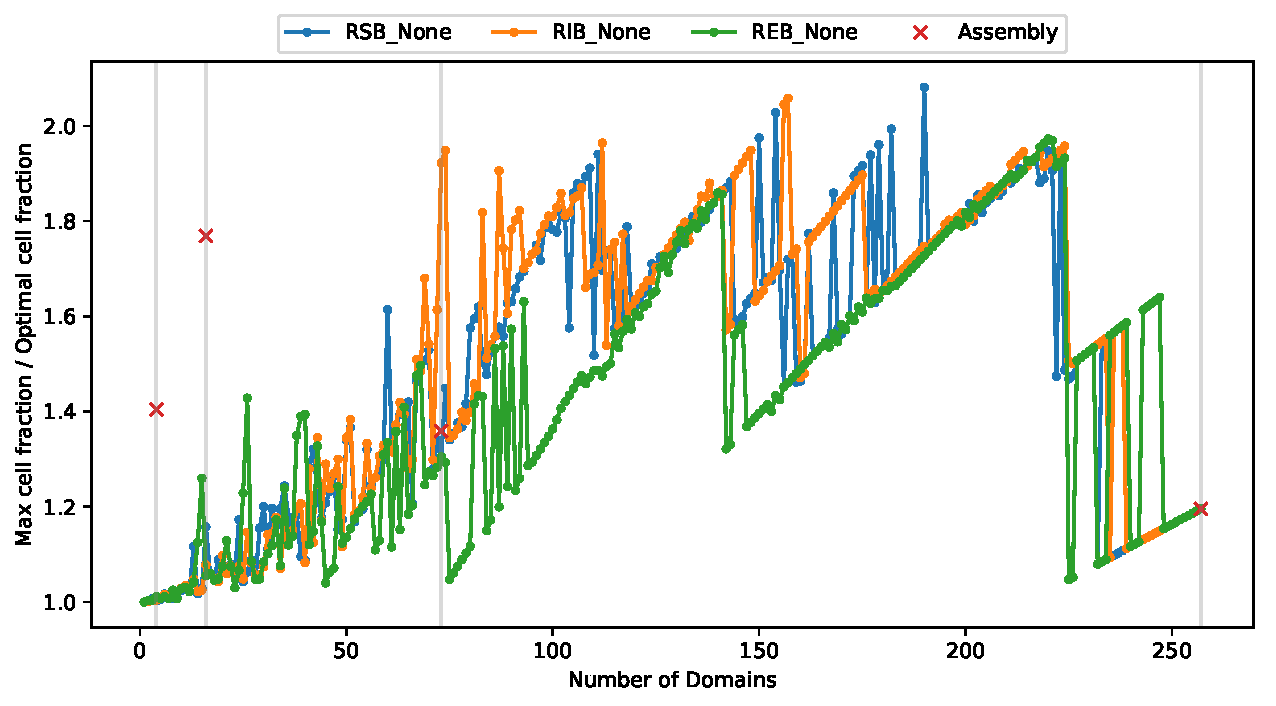
\includegraphics[width=\resultwidth]{results/2D/Size_to_Optimal}
          \caption{Ratio of largest fraction of cells to the optimal fraction of cells as a function of number of subdomains for each partitioning method without refinement.\label{fig:Spatial Decomposition:Max/Optimal Ratio}}
        \end{figure}
      }
      %%%%%%%%%%%%%%%%%%%%%%%%%%%%%%%%%%%%%%%%%%%%%%%%%%%%%%%%%%%%%%%%%%%%%%%%%%
      % Communication
      %%%%%%%%%%%%%%%%%%%%%%%%%%%%%%%%%%%%%%%%%%%%%%%%%%%%%%%%%%%%%%%%%%%%%%%%%%
      \subsubsection{Communication}{\label{sssec:Communication}
        In MPACT, parallel boundary conditions are communicated concurrently.
        However, the measurement of communication time includes any time spent waiting for other subdomains to complete their calculations.
        Generally, the time spent sending or receiving parallel boundary conditions is relatively small.
        This time is expected to increase with the weight of edges cut by parallel boundaries.

        \Cref{fig:Spatial Decomposition:2D Communication} shows that the number of edges cut increases as the number of domains increases.
        This indicates that time sending and receiving parallel boundary conditions is expected to increase with the number of subdomains.
        As the number of subdomains increases, the time spent sending and receiving parallel boundary conditions is expected to increase as more data is communicated.
        However, the time difference between the slowest and fastest subdomains decreases, so the overall communication time measurement is expected to decrease.
        Because subdomains in the assembly-based decomposition are rectangular, the number of edges cut is typically lower than in the graph partitioning methods.

        \begin{figure}
          \centering
          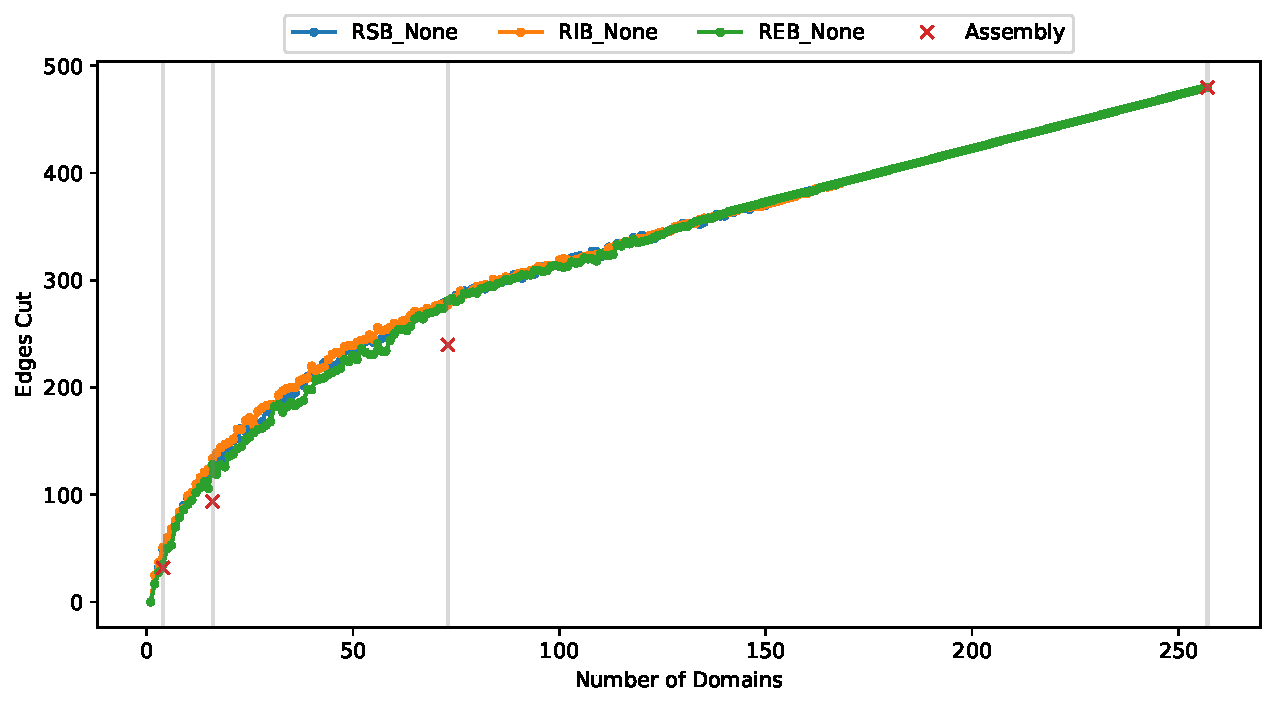
\includegraphics[width=\resultwidth]{results/2D/Edges_Cut}
          \caption{Number of edges cut as a fraction of number of domains for each partitioning method without refinement. \label{fig:Spatial Decomposition:2D Communication}}
        \end{figure}
      }
      %%%%%%%%%%%%%%%%%%%%%%%%%%%%%%%%%%%%%%%%%%%%%%%%%%%%%%%%%%%%%%%%%%%%%%%%%%
      % MPACT Results
      %%%%%%%%%%%%%%%%%%%%%%%%%%%%%%%%%%%%%%%%%%%%%%%%%%%%%%%%%%%%%%%%%%%%%%%%%%
      \subsubsection{MPACT Results}{\label{sssec:MPACT Results}
        As expected, the total and \ac{MOC} run-times are highly correlated with the largest fraction of cells in any subdomain, as shown in \cref{fig:Spatial Decomposition:Runtime Correlation}.
        Both total and \ac{MOC} run-times are very highly correlated with the largest fraction of cells in a subdomain, indicating that this metric can be used to estimate the relative run-times of decompositions.
        The assembly-based decomposition method was not used in this correlation, as there are only a few data points available.

        \begin{figure}
          \centering
          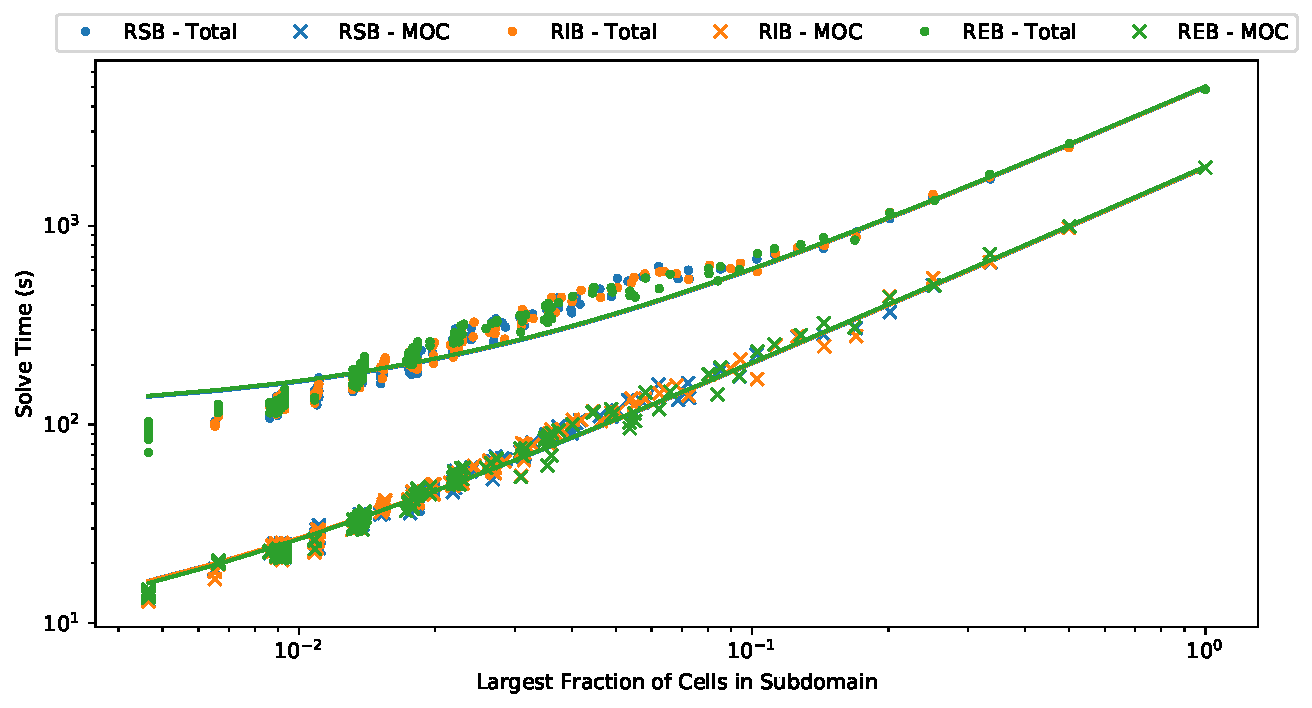
\includegraphics[width=\resultwidth]{results/2D/Run_Time_Fraction_Correlation}
          \caption{Correlation of total and \ac{MOC} run-times to the largest fraction of cells in a subdomain for each partitioning method. \label{fig:Spatial Decomposition:Runtime Correlation}}
        \end{figure}

        Utilization of computational resources is also an important aspect for a high performance simulation code; this can be measured by the parallel efficiency.
        The total parallel efficiency is shown in \cref{fig:Spatial Decomposition:Parallel Efficiency} for each decomposition method.
        As the core becomes more decomposed, the parallel efficiency drops off rapidly, approaching around 20\%.
        Generally, the graph partitioning methods result in similar parallel efficiency, though the \ac{REB} method appears to give very slightly higher efficiency in many cases.
        The assembly-based decomposition method has significantly lower parallel efficiency when there are few subdomains.
        However, for the moderately decomposed problem (73 subdomains) the assembly-based decomposition method results in significantly higher parallel efficiency.
        This was not initially expected, as the largest subdomain has a cell fraction similar to that of the graph partitioning methods.

        \begin{figure}
          \centering
          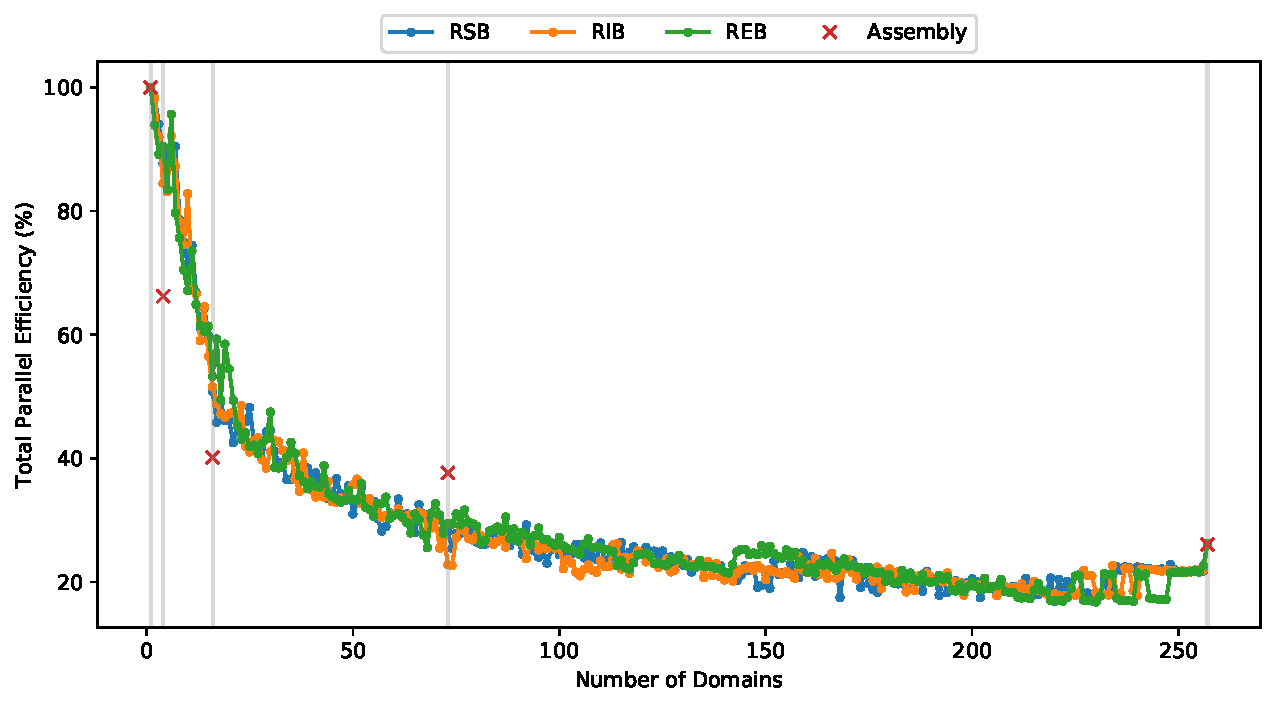
\includegraphics[width=\resultwidth]{results/2D/Total_Parallel_Efficiency}
          \caption{The total parallel efficiency for each partitioning method as a function of the number of domains. \label{fig:Spatial Decomposition:Parallel Efficiency}}
        \end{figure}

        As parallel boundary conditions have a more significant effect on the solution within each subdomain, the convergence rate decreases.
        This occurs as subdomains become smaller (geometrically), or as they become more ``jagged.''
        These jagged parallel boundaries cause re-entrant rays, in which a single ray in the \ac{MOC} will re-enter the subdomain after leaving.
        These re-entrant rays will \emph{not} occur in the assembly-based decomposition, because subdomains are forced to be rectangular.
        This can be observed in \cref{fig:Spatial Decomposition:5a-2d example decomp}.
        The number of \ac{MOC} iterations required for convergence in each case is shown in \cref{fig:Spatial Decomposition:Convergence}.
        There is not a significant increase in the number of outer iterations as the subdomains become smaller, this is consistent with previous results in parallel accelerated transport calculations \cite{Kelley2012,Stimpson2014,Kochunas2014}.
        The increase in number of iterations would be expected to be much more significant in an unaccelerated transport calculation.
        It may be possible to consider spectral information, such as subdomain optical thickness or scattering ratios, during decomposition to allow for a smaller increase in required iterations; however, this will only have an effect at moderately decomposed problems.

        \begin{figure}
          \centering
          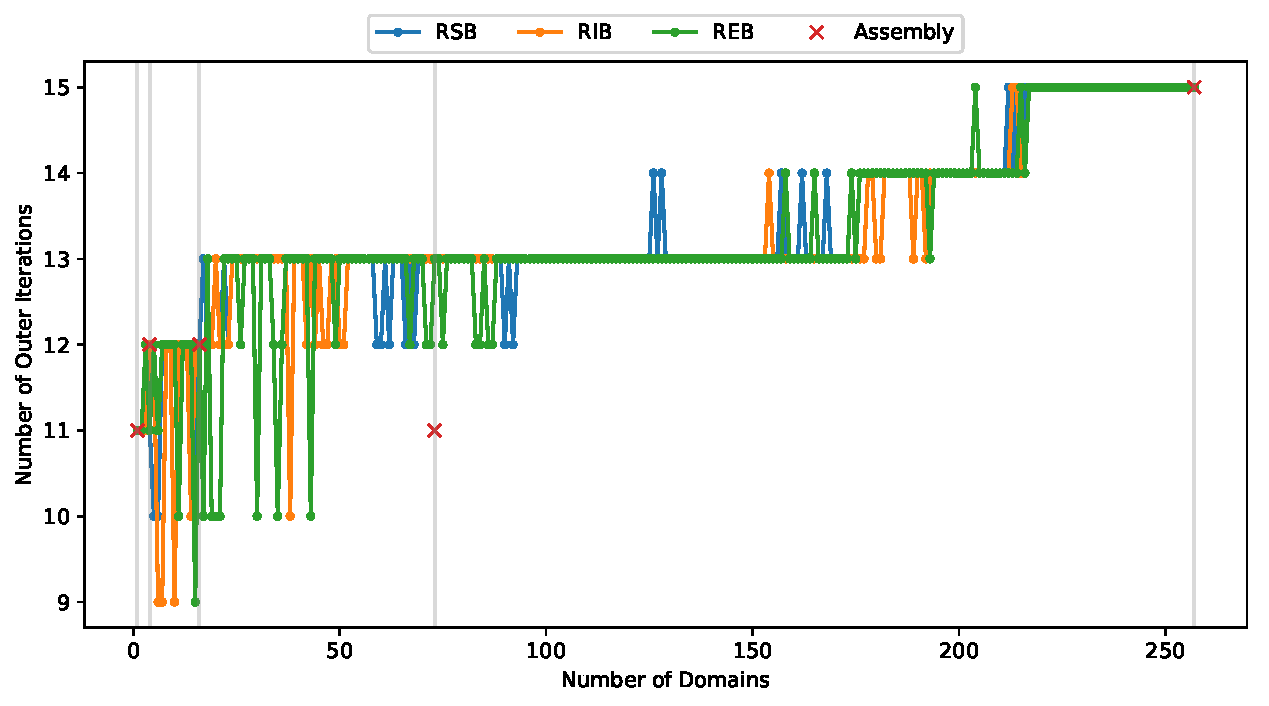
\includegraphics[width=\resultwidth]{results/2D/Convergence_Rates}
          \caption{The number of iterations used by each decomposition method as a function of the number of subdomains. \label{fig:Spatial Decomposition:Convergence}}
        \end{figure}

        By examining the parallel efficiency of \emph{runtime per iteration} these spectral effects are eliminated and the scaling of the solvers in parallel can be determined.
        As shown in \cref{fig:Spatial Decomposition:Scaled Parallel Efficiency}, the total parallel efficiency per iteration decreases as the core becomes more decomposed, limiting toward 25\%.
        However, if only the \ac{MOC} solver time is being examined, the parallel efficiency per iteration decreases at a much slower rate as shown in \cref{fig:Spatial Decomposition:Scaled MOC Parallel Efficiency}.
        This indicates that the \ac{MOC} solver in MPACT is highly efficient in parallel, and that other components of MPACT are the bottleneck in parallel simulations.
        Furthermore, for both total and \ac{MOC} run-times, the graph partitioning methods give comparable parallel efficiencies.
        The assembly-based decomposition method still results in lower efficiency when using few subdomains, but for high numbers of subdomains, it is comparable with the graph partitioning methods.

        \begin{figure}
          \centering
          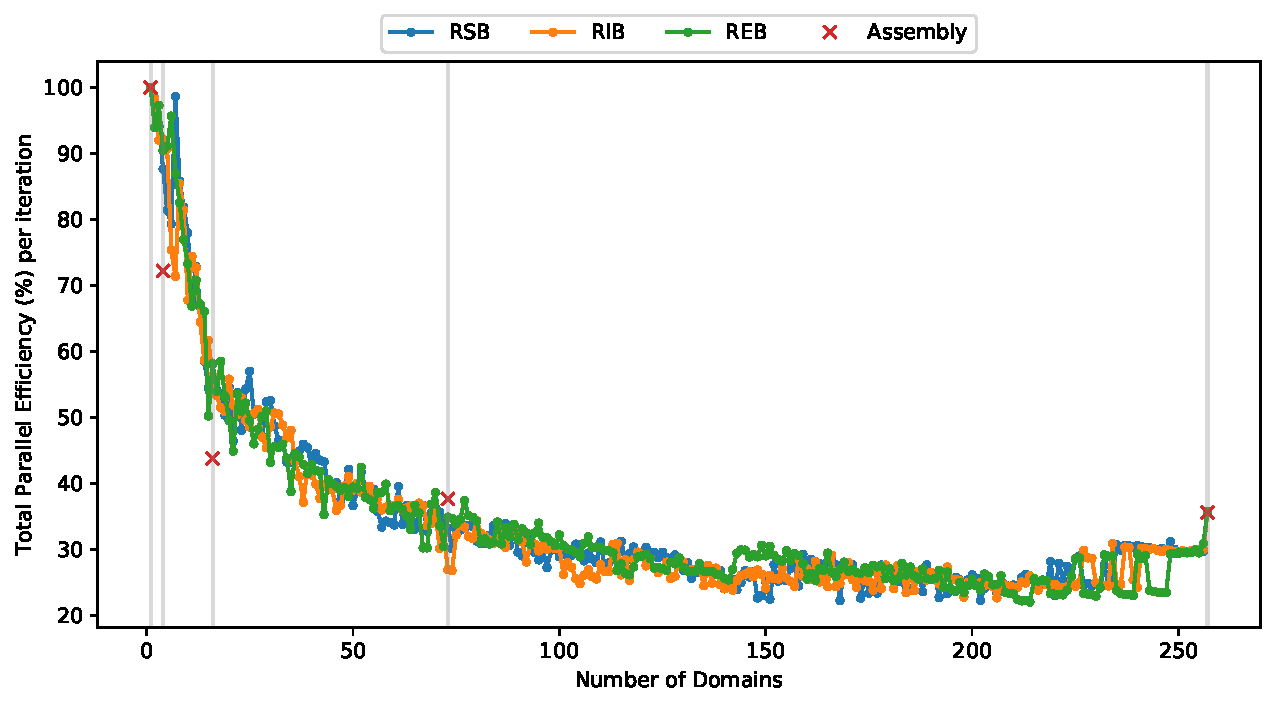
\includegraphics[width=\resultwidth]{results/2D/Scaled_Total_Parallel_Efficiency}
          \caption{The total parallel efficiency per iteration for each partitioning method as a function of the number of domains. \label{fig:Spatial Decomposition:Scaled Parallel Efficiency}}
        \end{figure}

        \begin{figure}
          \centering
          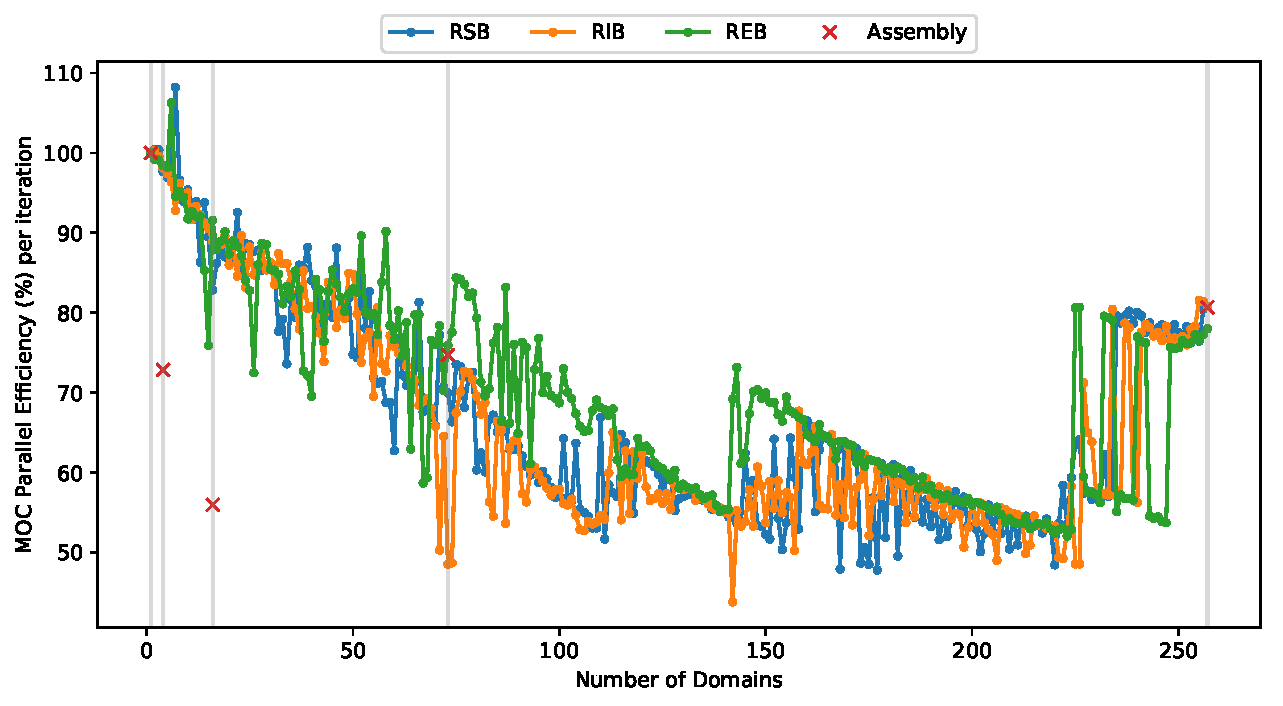
\includegraphics[width=\resultwidth]{results/2D/Scaled_MOC_Parallel_Efficiency}
          \caption{The \ac{MOC} parallel efficiency per iteration for each partitioning method as a function of the number of domains. \label{fig:Spatial Decomposition:Scaled MOC Parallel Efficiency}}
        \end{figure}


        Finally, the ratio of the optimal cell fraction to the maximum cell fraction is expected to be proportional to the parallel efficiency per iteration of the \ac{MOC} solver.
        As shown in \cref{fig:Spatial Decomposition:MOC Parallel Efficiency Correlation}, the parallel efficiency is correlated with the the ratio of optimal-to-maximum cell fractions, though it is not correlated as strongly as the runtime with the maximum cell fraction.
        This indicates that this ratio can be used to estimate the parallel efficiency of the \ac{MOC} solver for a decomposition.
        Even isolating the effect due to increased numbers of iterations, there is a significant spread in parallel efficiency as a function of the optimal to maximum cell fraction ratio; this can be explained by the fact that significantly different numbers of domains (processes) can result in similar fractions.
        This is clearly observed in \cref{fig:Spatial Decomposition:Max/Optimal Ratio}.

        \begin{figure}
          \centering
          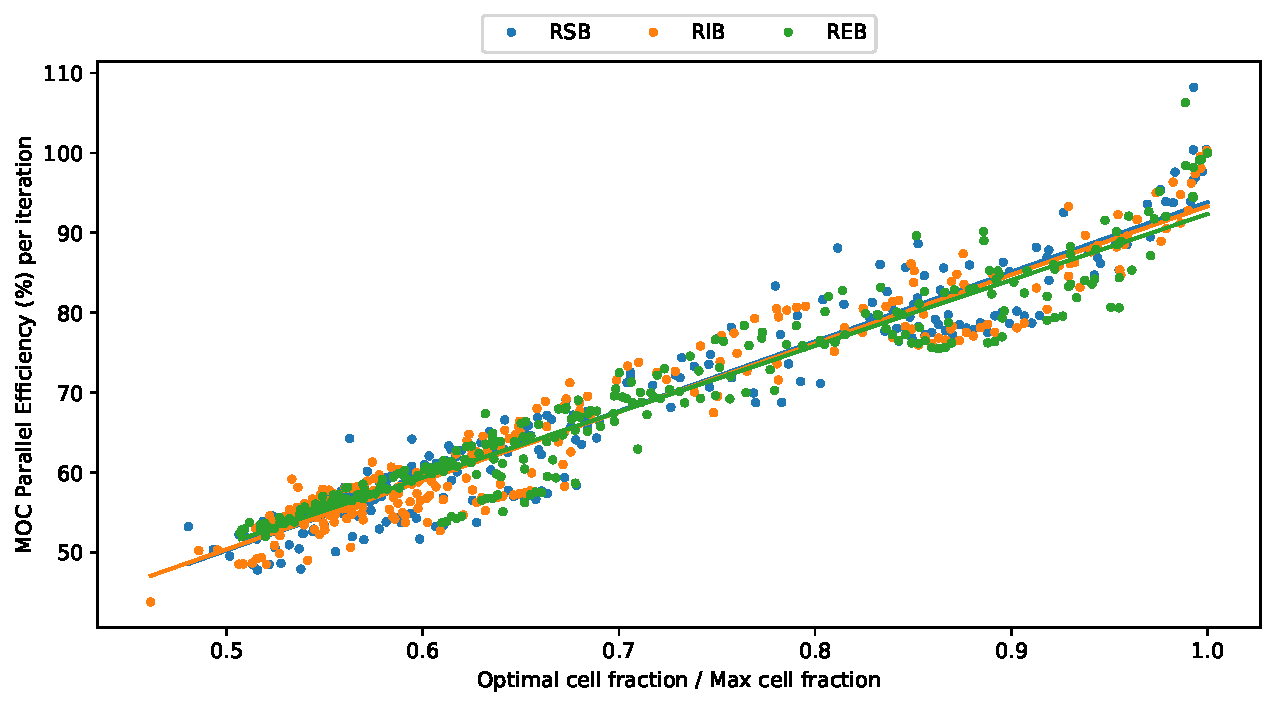
\includegraphics[width=\resultwidth]{results/2D/MOC_Parallel_Efficiency_Correlation}
          \caption{Correlation of the \ac{MOC} parallel efficiency per iteration and the ratio of optimal and maximum cell fractions for each of the partitioning methods. \label{fig:Spatial Decomposition:MOC Parallel Efficiency Correlation}}
        \end{figure}
      }
      %%%%%%%%%%%%%%%%%%%%%%%%%%%%%%%%%%%%%%%%%%%%%%%%%%%%%%%%%%%%%%%%%%%%%%%%%%
      % CMFD Acceleration
      %%%%%%%%%%%%%%%%%%%%%%%%%%%%%%%%%%%%%%%%%%%%%%%%%%%%%%%%%%%%%%%%%%%%%%%%%%
      \subsubsection{CMFD Acceleration}{\label{sssec:CMFD Acceleration}
        In MPACT, the two main solvers contributing to runtime of a steady-state eigenvalue calculation are the \ac{MOC} solver and \ac{CMFD} acceleration, each of which is parallelized using the same computational resources.
        From \cref{fig:Spatial Decomposition:Fractional Runtimes}, the \ac{MOC} and \ac{CMFD} solvers take similar amounts of time in serial; however, as more subdomains are used, the fractional runtime of \ac{CMFD} increases to almost 70\% of the total.
        This indicates that the parallel efficiency is quite low for MPACT's \ac{CMFD} linear system solvers, which heavily leverage PETSc \cite{Petsc} for parallelism.

        \begin{figure}
          \centering
          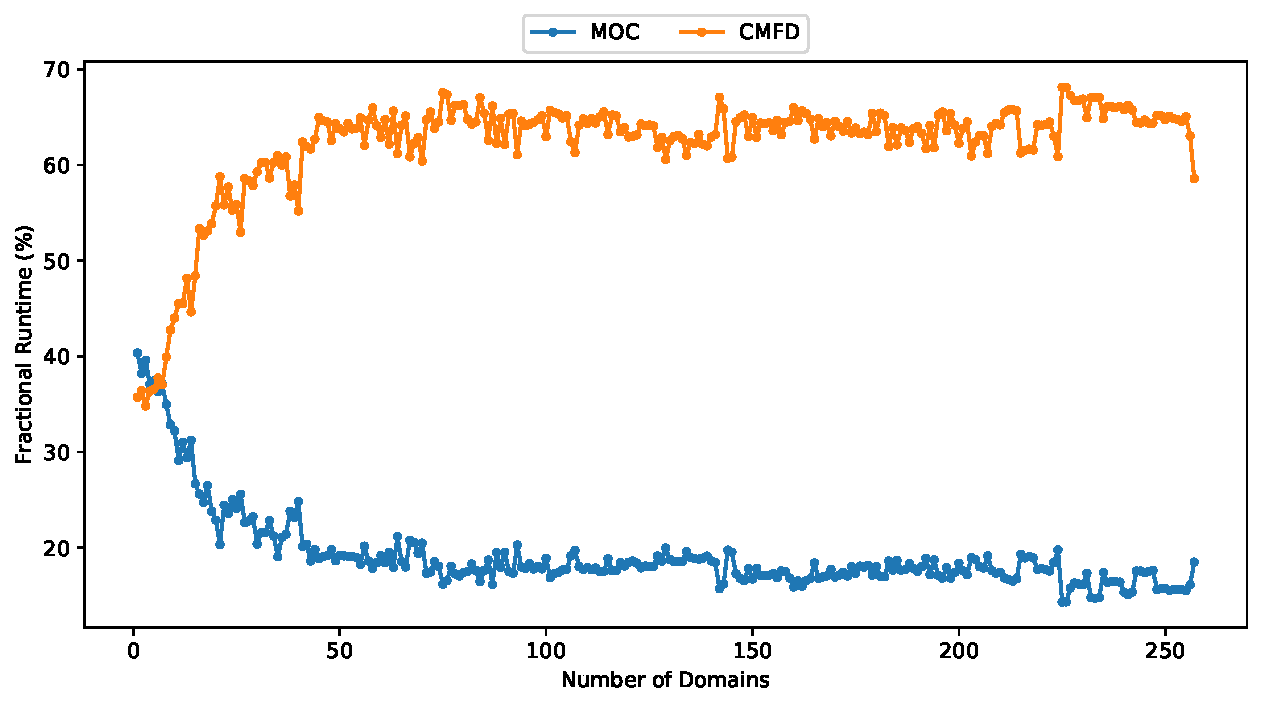
\includegraphics[width=\resultwidth]{results/2D/Fractional_Runtimes}
          \caption{Fractional runtime of the \ac{MOC} solver and \ac{CMFD} acceleration method in MPACT for varying number of domains with the \ac{REB} partitioning method. \label{fig:Spatial Decomposition:Fractional Runtimes}}
        \end{figure}

        Similar as the number of outer transport iterations, as subdomains become smaller, it is expected the \ac{CMFD} linear system will require more iterations for convergence; this is shown for the \ac{REB} partitioning method in \cref{fig:Spatial Decomposition:CMFD Efficiency Summary}.
        This is because the pre-conditioner used in MPACT is less efficient with more domains.
        However, by considering the parallel efficiency per inner iteration, these convergence effects can be eliminated, and the parallel scaling of the linear system solvers can be examined.
        \Cref{fig:Spatial Decomposition:CMFD Efficiency Summary} shows that the parallel efficiency of the linear system solvers used in MPACT for \ac{CMFD} calculations is quite low, limiting to around 30\%.
        By using a linear system solver that has better parallel scaling \cite{Hao2018}, the overall parallel efficiency of MPACT may be increased.
        However, these results also indicate that the parallel efficiency is, in part, lowered by spectral effects, that will not be eliminated by a more efficient parallel linear solver.

        \begin{figure}
          \centering
          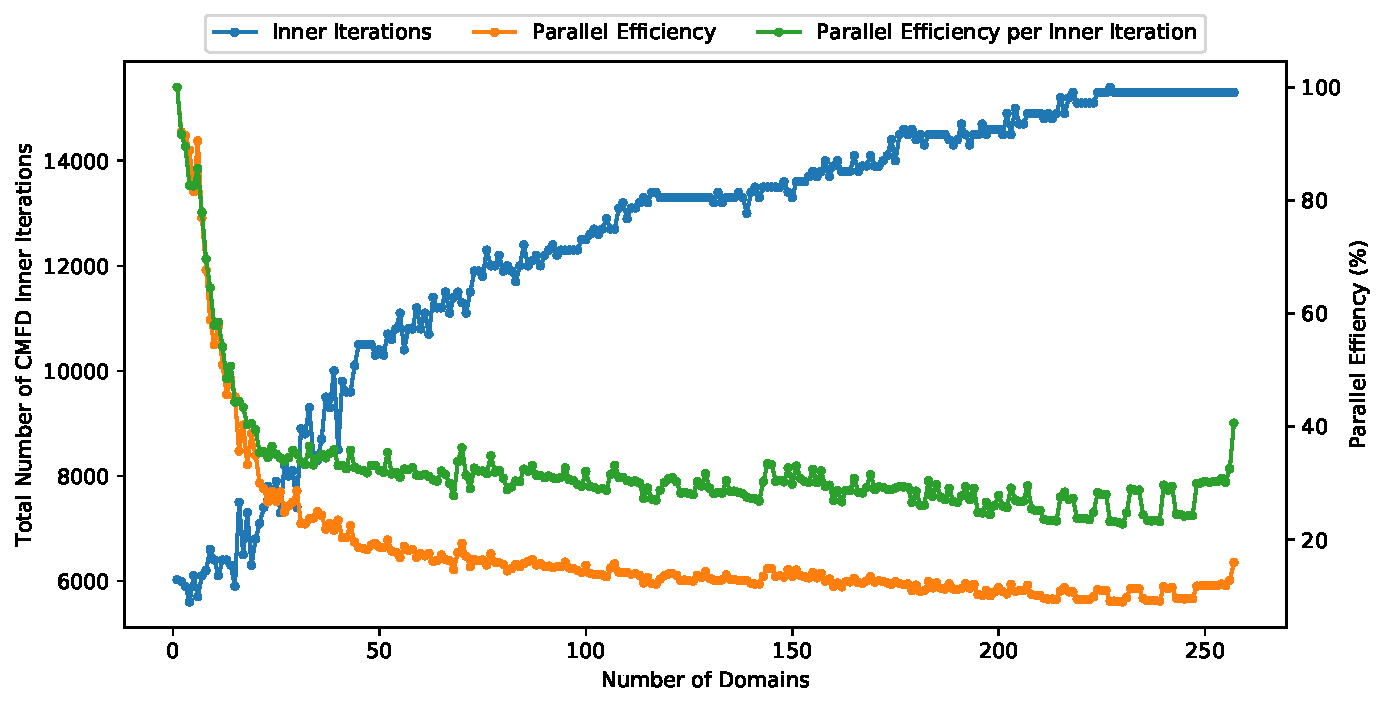
\includegraphics[width=\resultwidth]{results/2D/CMFD_Efficiency_Summary.pdf}
          \caption{The total number of \ac{CMFD} inner iterations, parallel efficiency, and parallel efficiency per inner iteration for varying number of domains with the \ac{REB} partitioning method. \label{fig:Spatial Decomposition:CMFD Efficiency Summary}}
        \end{figure}
      }
    }
    %%%%%%%%%%%%%%%%%%%%%%%%%%%%%%%%%%%%%%%%%%%%%%%%%%%%%%%%%%%%%%%%%%%%%%%%%%%%
    % 3-D Results
    %%%%%%%%%%%%%%%%%%%%%%%%%%%%%%%%%%%%%%%%%%%%%%%%%%%%%%%%%%%%%%%%%%%%%%%%%%%%
    \subsection{3-D Results}{\label{ssec:Spatial Decomposition:3-D Results}
      As shown in \cref{ssec:Spatial Decomposition:2-D Results}, decomposition metrics can be used to estimate the runtime and parallel efficiency without needing to run the simulations.
      There are different approaches to decomposition in 3-D; these are discussed in more detail in \cref{sec:Spatial Decomposition:Applications for MPACT}.
      Decompositions were performed without refinement for three different 3-D decomposition schemes:  \ac{ARA}, \ac{RA}, and \ac{UR}.
      Given fewer restrictions, the resulting decompositions were expected to be more balanced.
      Decompositions were performed on VERA progression problem 5a-0 in 3-D \cite{VERAProblems} with 58 axial planes, but the simulations for this problem were not run.

      The ratio of maximum cell fraction to optimal cell fraction can easily be converted to the maximum cell fraction by dividing by $N$.
      For brevity, only this load balance metric is shown herein.
      The resulting decompositions from the \ac{ARA} approach are very similar to those in the 2-D case.
      Just as in the 2-D case, the maximum-to-optimal cell fraction ratio is lowest for the \ac{REB} method as compared to the other partitioning methods for many cases, as seen in \cref{fig:Spatial Decomposition:3D AR Max. to Optimal Cell Ratio}.
      This indicates that, barring any differences in the number of iterations, the \ac{REB} method is expected to have slightly higher parallel efficiencies.

      \begin{figure}
        \centering
        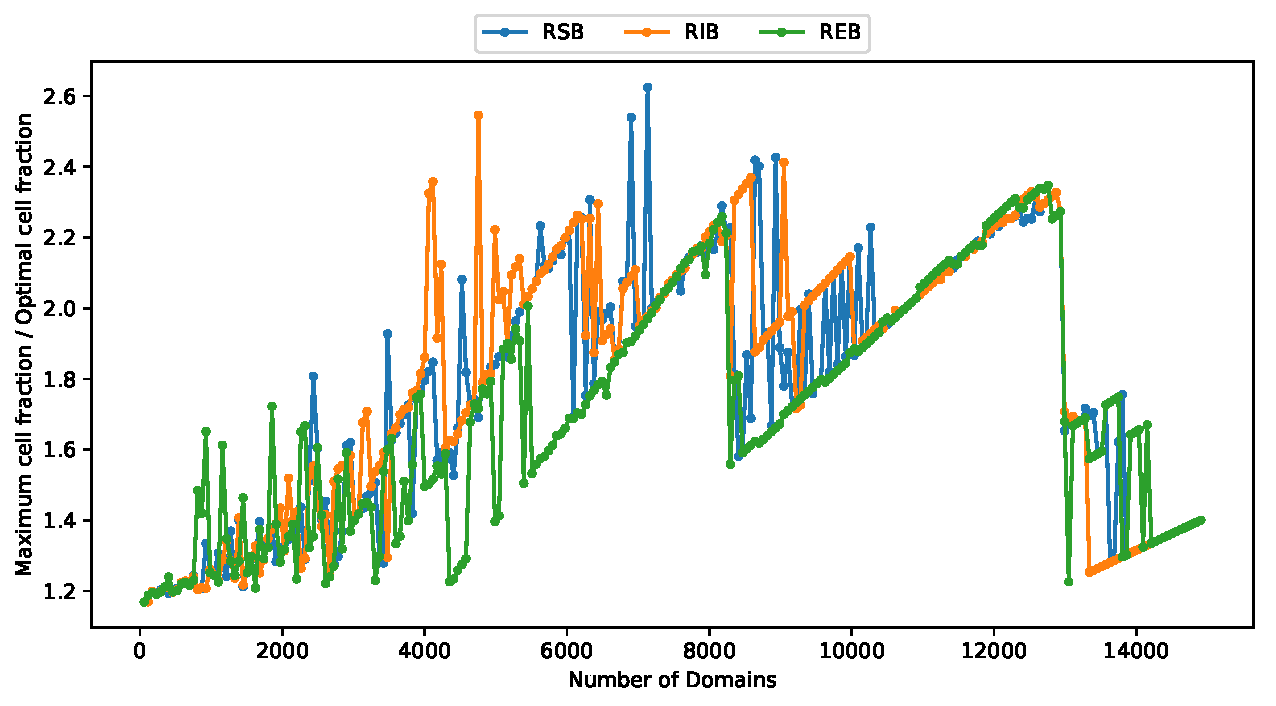
\includegraphics[width=\resultwidth]{results/3D/AxialRadial_Comparison_Ratio}
        \caption{Maximum-to-optimal cell fraction ratio for each partitioning method as a function of number of domains in the \acf{ARA} scheme. \label{fig:Spatial Decomposition:3D AR Max. to Optimal Cell Ratio}}
      \end{figure}

      In the \ac{RA} scheme, a separate decomposition is performed for each axial plane, with an appropriate number of subdomains based on the number of cells in the plane.
      Unlike in the 2-D case, the \ac{REB} method seems to perform significantly worse than the other two methods for low numbers of subdomains.
      For highly decomposed cores, the \ac{REB} method seems to perform slightly better than the other partitioning methods.
      Additionally, by comparing the magnitude of the ratios in \cref{fig:Spatial Decomposition:3D R Max. to Optimal Cell Ratio} and \cref{fig:Spatial Decomposition:3D AR Max. to Optimal Cell Ratio}, it is clear that the \ac{RA} approach typically has less imbalance.

      \begin{figure}
        \centering
        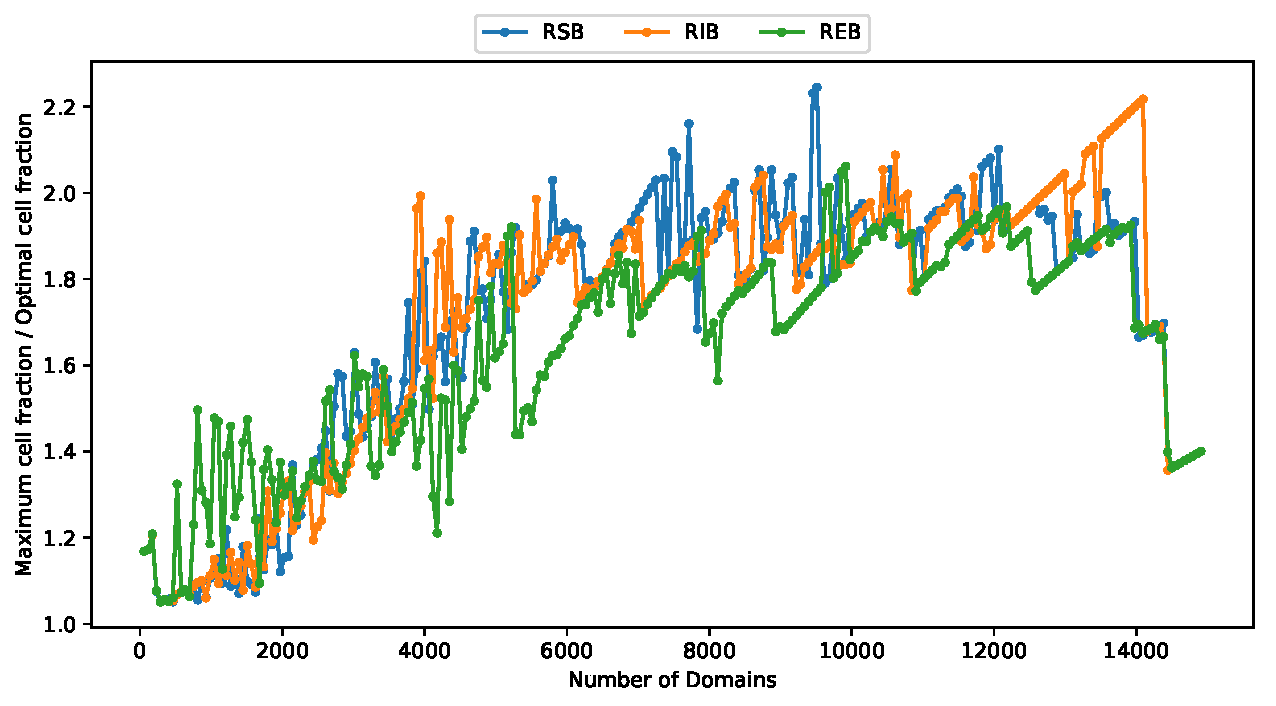
\includegraphics[width=\resultwidth]{results/3D/Radial_Comparison_Ratio}
        \caption{Maximum-to-optimal cell fraction ratio for each partitioning method as a function of number of domains in the \acf{RA} scheme. \label{fig:Spatial Decomposition:3D R Max. to Optimal Cell Ratio}}
      \end{figure}

      Finally, the \ac{UR} approach decomposes the 3-D core by directly abstracting the entire core into a graph.
      The \ac{REB} method is significantly more imbalanced than other methods for lower numbers of subdomains; however, for highly decomposed cores, the \ac{REB} method outperforms the other methods, as shown in \cref{fig:Spatial Decomposition:3D U Max. to Optimal Cell Ratio}.
      Additionally, for highly decomposed problems, both the \ac{RSB} and \ac{RIB} methods seem to have worse balance when using the \ac{UR} scheme compared to the \ac{RA} scheme.

      \begin{figure}
        \centering
        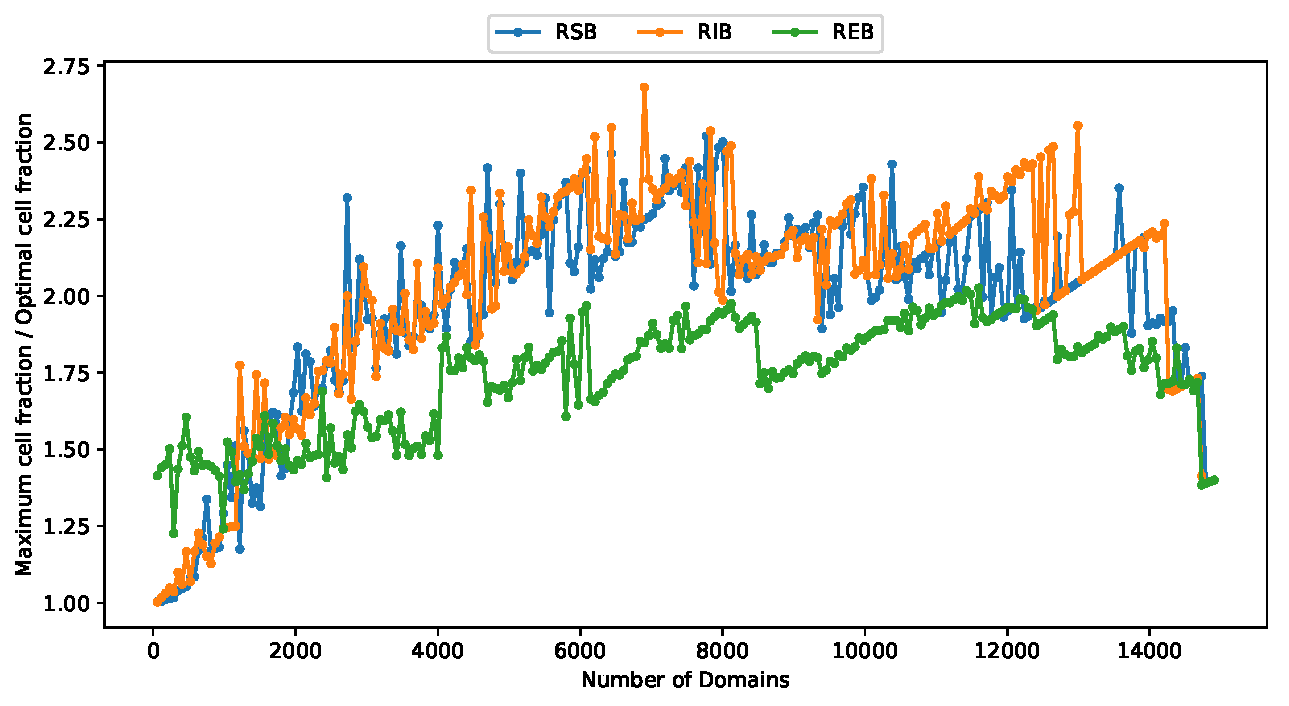
\includegraphics[width=\resultwidth]{results/3D/General_Comparison_Ratio}
        \caption{Maximum-to-optimal cell fraction ratio for each partitioning method as a function of number of domains in the \acf{UR} scheme. \label{fig:Spatial Decomposition:3D U Max. to Optimal Cell Ratio}}
      \end{figure}

      The approach currently used in MPACT is the axially and radially aligned 3-D decomposition scheme.
      If other approaches were to be used, the implementation of parallel communication in the 2D-1D method would need to be made more general.
      To justify these changes, the less restricted approaches would need to offer significant advantages over the current approach.
      \Cref{fig:Spatial Decomposition:RSB 3D Comparison,fig:Spatial Decomposition:RIB 3D Comparison,fig:Spatial Decomposition:REB 3D Comparison} examine the maximum cell fraction of each scheme relative to the current scheme.
      The smaller the relative maximum cell fraction, the lower the expected runtime will be.

      For most applications, reactor cores in MPACT are not highly decomposed.
      At maximum, on the order of 30 subdomains per axial plane are unrestricted.
      In this context, modestly decomposed cores are defined as those with fewer than 2,000 subdomains; otherwise, the core is considered highly decomposed.
      For the \ac{RSB} and \ac{RIB} methods, the \ac{RA} approach is expected to give 10\% better performance than the \ac{ARA} approach on average.
      For highly decomposed cases, these partitioning methods are only expected to give an average of 2 -- 3\% better performance.
      On average, the \ac{UR} approach is expected to give \emph{worse} performance by more than 10\% using these partitioning methods.
      However, for the \ac{REB} partitioning method, the \ac{RA} approach is only expected to give 3\% better performance on average.
      Typically, the \ac{UR} approach is still expected to result in worse performance.
      This may be a result of the problem examined in this work which had axial planes that were fairly well balanced.
      By giving the graph partitioning methods more degrees of freedom the heuristic graph partitioning methods perform worse overall.
      Multi-level partitioning methods reduce the degrees of freedom during coarsening and may be more appropriate in these cases.

      \begin{figure}
        \centering
        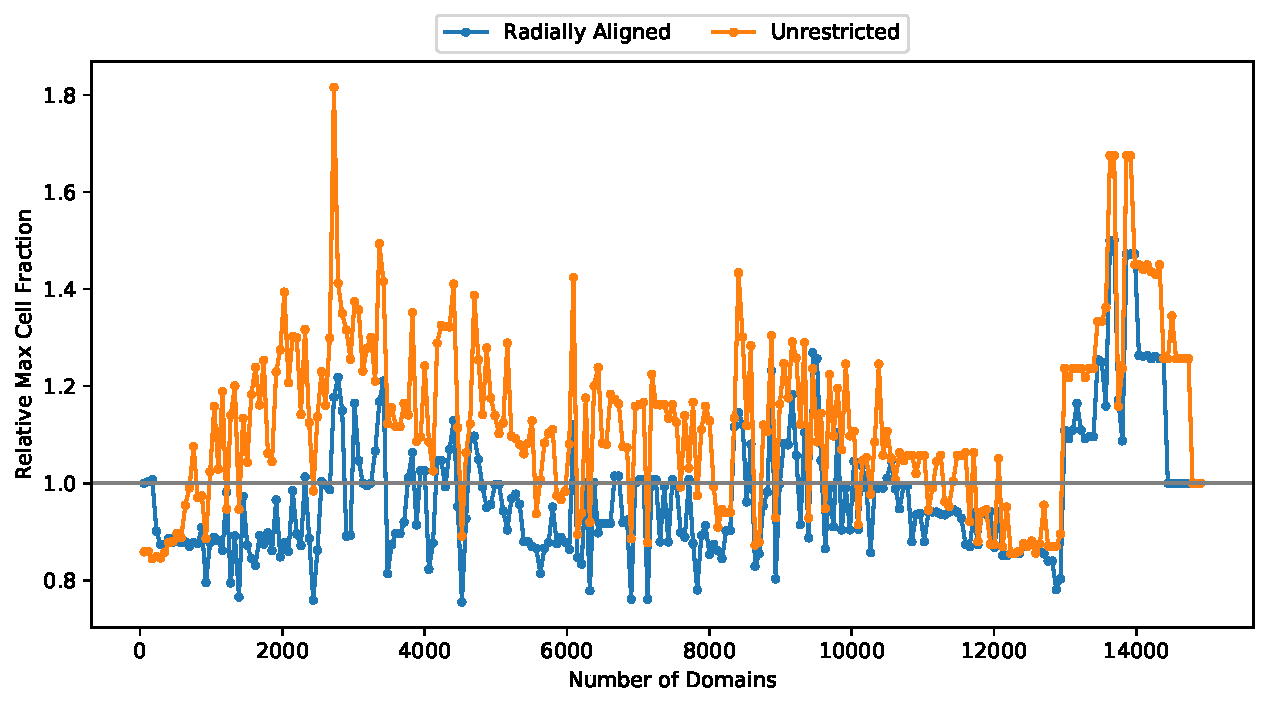
\includegraphics[width=\resultwidth]{results/3D/RSB_Comparison}
        \caption{Maximum cell fraction relative to the \acf{ARA} approach for the \ac{RSB} partitioning method. \label{fig:Spatial Decomposition:RSB 3D Comparison}}
      \end{figure}
      \begin{figure}
        \centering
        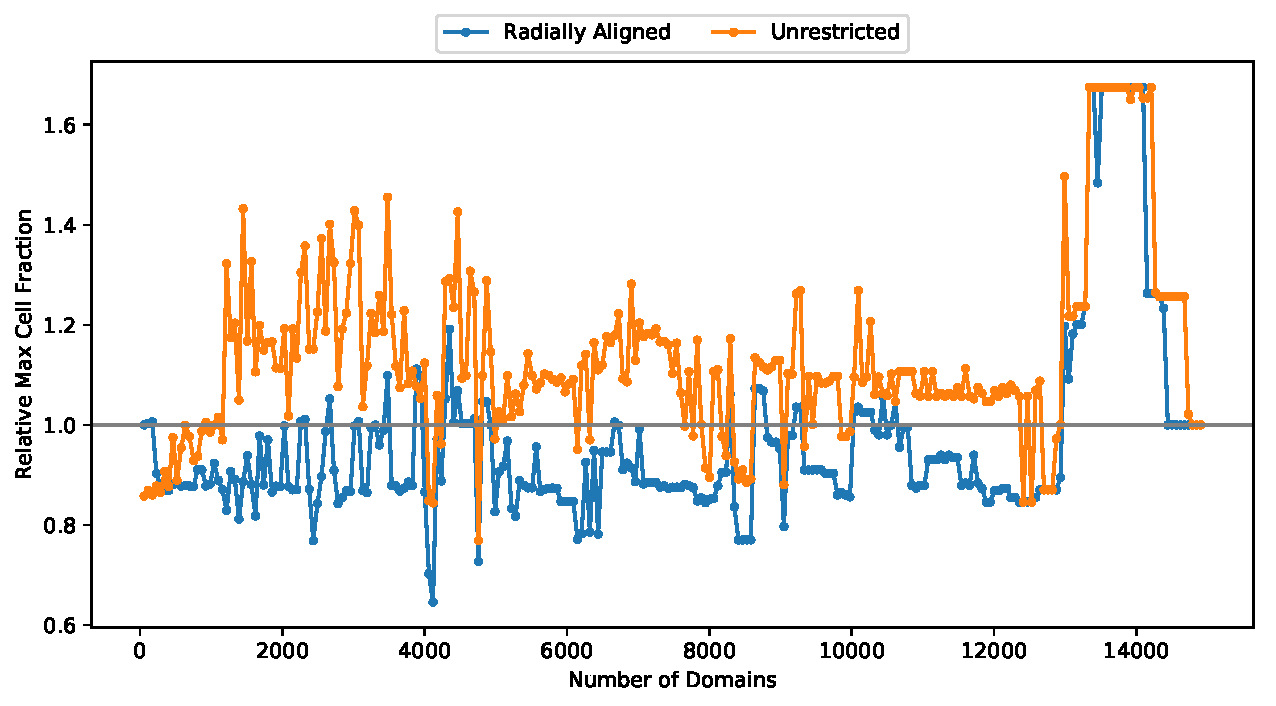
\includegraphics[width=\resultwidth]{results/3D/RIB_Comparison}
        \caption{Maximum cell fraction relative to the \acf{ARA} approach for the \ac{RIB} partitioning method. \label{fig:Spatial Decomposition:RIB 3D Comparison}}
      \end{figure}
      \begin{figure}
        \centering
        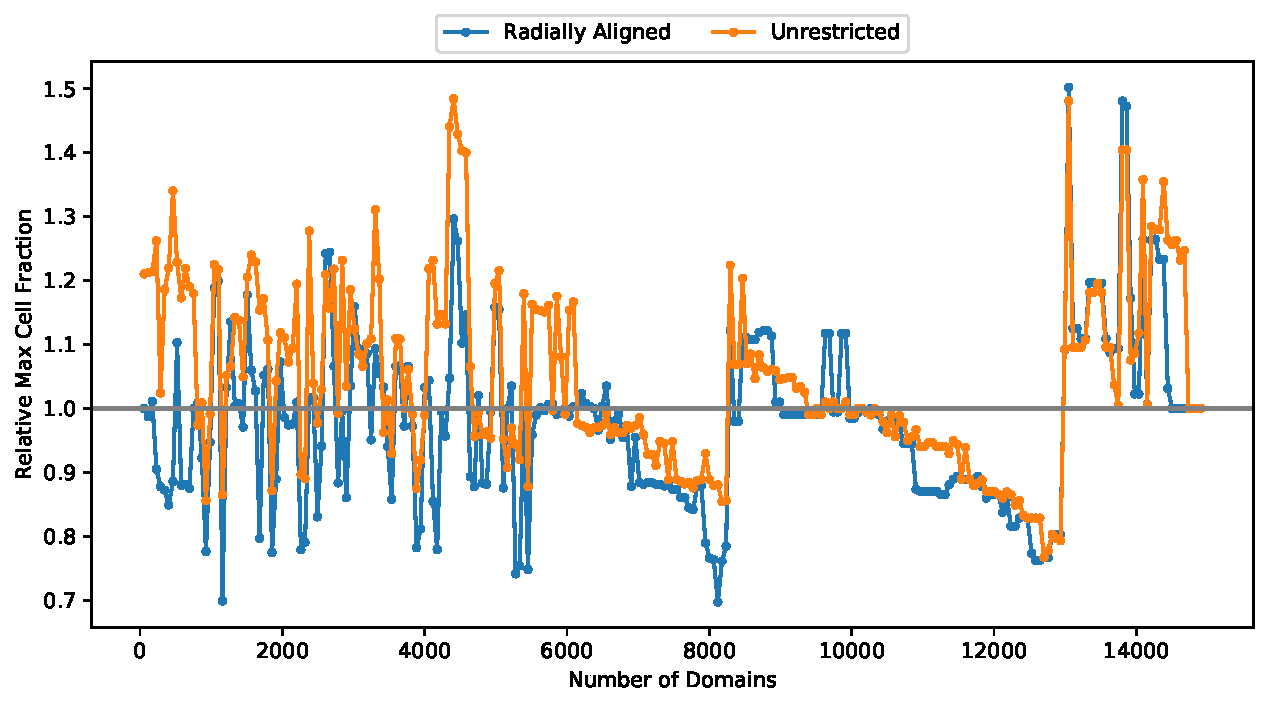
\includegraphics[width=\resultwidth]{results/3D/REB_Comparison}
        \caption{Maximum cell fraction relative to the \acf{ARA} approach for the \ac{REB} partitioning method. \label{fig:Spatial Decomposition:REB 3D Comparison}}
      \end{figure}
    }
  }
  %%%%%%%%%%%%%%%%%%%%%%%%%%%%%%%%%%%%%%%%%%%%%%%%%%%%%%%%%%%%%%%%%%%%%%%%%%%%%%
  % Partition Refinement Methods
  %%%%%%%%%%%%%%%%%%%%%%%%%%%%%%%%%%%%%%%%%%%%%%%%%%%%%%%%%%%%%%%%%%%%%%%%%%%%%%
  \section{Partition Refinement}{\label{sec:Spatial Decomposition:Partition Refinement}
    %%%%%%%%%%%%%%%%%%%%%%%%%%%%%%%%%%%%%%%%%%%%%%%%%%%%%%%%%%%%%%%%%%%%%%%%%%%%
    % Partition Refinement Methods
    %%%%%%%%%%%%%%%%%%%%%%%%%%%%%%%%%%%%%%%%%%%%%%%%%%%%%%%%%%%%%%%%%%%%%%%%%%%%
    \subsection{Partition Refinement Methods}{\label{ssec:Spatial Decomposition:Partition Refinement Methods}
      The Kernighan-Lin algorithm \cite{Kernighan1970} is often described as one of the earliest developed graph partitioning algorithms; however, the algorithm does not actually create a partitioning of the graph, it improves, or refines, the quality by reducing the number of edges cut between existing partitions \cite{Elsner1997}.
      Therefore, in this work, this method and a modified version of it are called \emph{refinement methods}.

      As suggested by Pothen \cite{Pothen1989}, the \ac{RSB} method or other partitioning methods can create a high quality initial partitioning to use in the Kernighan-Lin algorithm.
      Significant improvements have been made to the efficiency of the original Kernighan-Lin algorithm \cite{Fiduccia1982}; however, the graphs of concern in this work are relatively small, and graph decomposition time is negligible when compared to the overall simulation runtime.
      Two partition refinement methods were examined: the Kernighan-Lin algorithm \cite{Kernighan1970} and a modification to the Kernighan-Lin algorithm which takes some geometric information of the graph into account \cite{Fitzgerald2017}.

      The investigated partition refinement algorithms reduce the weight of edges cut between two partitions by swapping vertex pairs between the partitions iteratively.
      The original Kernighan-Lin algorithm operates entirely on the connectivity of the graph, while the modified Spatial Kernighan-Lin algorithm uses both connectivity and geometric information from the graph.

      For each vertex in the graph, $D$ is defined as
      \begin{equation}
          \label{eq:Spatial Decomposition:KL D}
          D_i \equiv E_{E,i} - E_{I,i},
      \end{equation}
      where $E_{E,i}$ is the sum of edge weights from vertex $i$ connecting with vertices outside the partition containing vertex $i$, and $E_{I,i}$ is the sum of edge weights from vertex $i$ connecting with vertices within the partition containing vertex $i$.
      The reduction in communication or ``gain,'' from swapping a pair of vertices $(a,b)$ is defined as
      \begin{equation}
          \label{eq:Spatial Decomposition:KL gain}
          g_{(a,b)} \equiv D_a + D_b - 2c_{a,b}.
      \end{equation}

      The Kernighan-Lin algorithm, given in \cref{alg:Kernighan-Lin}, is a greedy algorithm, in that it will swap a pair $(a,b)$ with maximal $g$ at the current step.
      The idea is that by doing this iteratively, the algorithm will lead to a minimized cut-size; in reality, the algorithm will often get stuck in local minima that do not have a global minimized cut-size.
      Additionally, there may be multiple pairs $(a,b)$ with the same maximal gain value: the algorithm will only consider one of these pairs.

      The Spatial Kernighan-Lin algorithm, given in \cref{alg:Spatial Kernighan-Lin}, is an adaptation of the Kernighan-Lin algorithm that accounts for the multiple pairs with maximal gain.
      This algorithm was developed as part of this work, in an attempt to improve the original Kernighan-Lin algorithm for this specific application.
      This algorithm prioritizes vertex pairs which are geometrically distant from one another.
      The idea behind this modification is that to minimize the edge-cut, the cut should be as straight as possible.
      By prioritizing distant vertex pairs, the bisector is typically ``straightened out''; this process can be likened to pulling on the ends of a string in order to straighten it.

      \begin{algorithm}
        \centering
        \caption{Kernighan-Lin Algorithm, with input graph $G(V,E)$, and vertex sets $A$ and $B$ within the graph.}
        \label{alg:Kernighan-Lin}
        \begin{algorithmic}[1]
          \Procedure{Kernighan-Lin}{$G(V,E), A, B$}
            \State{$g_m = 1$}
            \While{$g_m > 0$}
              \State{$W_A = \suml[i \in A]w_i$}
              \State{$W_B = \suml[i \in B]w_i$}
              \State{Compute $D \ \forall \ V$ (\Cref{eq:Spatial Decomposition:KL D})}
              \State{Let $a_v, b_v, g_v$ be empty sets}
              \For{$n=1$~to~$N/2$}
                \State{Find unmarked pair $(a,b)$ such that:
                    \begin{enumerate}[leftmargin=2.5cm]
                        \item{$a \in A$ and $b \in B$}
                        \item{$g$ is maximized (\Cref{eq:Spatial Decomposition:KL gain})}
                    \end{enumerate}
                }
                \State{$\widehat{W}_A = W_A + w_b - w_a$}
                \State{$\widehat{W}_B = W_B + w_a - w_b$}
                \If{MAX($W_A$, $W_B$) $\geq$ MAX($\widehat{W}_A, \widehat{W}_B$)}
                  \State{Append $a$ to $a_v$, $b$ to $b_v$, and $g$ to $g_v$}
                  \State{Update $D$ values as if $a,b$ have been swapped}
                  \State{$W_A = \widehat{W}_A$}
                  \State{$W_A = \widehat{W}_B$}
                \Else
                  \State{End search}
                \EndIf
              \EndFor
              \State{Find $k$ maximizing $g_m = \suml[i=1][k]g_v(i)$}
              \If{$g_m > 0$}
                \State{Exchange vertices in $a_v(1:k)$ and $b_v(1:k)$}
              \EndIf
            \EndWhile
          \EndProcedure
        \end{algorithmic}
      \end{algorithm}

      \begin{algorithm}
        \centering
        \caption{Spatial Kernighan-Lin Algorithm, with input graph $G(V,E)$, and vertex sets $A$ and $B$ within the graph.}
        \label{alg:Spatial Kernighan-Lin}
        \begin{algorithmic}[1]
          \Procedure{Spatial Kernighan-Lin}{$G(V,E), A, B$}
            \State{$g_m = 1$}
            \While{$g_m > 0$}
              \State{$W_A = \suml[i \in A]w_i$}
              \State{$W_B = \suml[i \in B]w_i$}
              \State{Compute $D \ \forall \ V$ (\Cref{eq:Spatial Decomposition:KL D})}
              \State{Let $a_v, b_v, g_v$ be empty sets}
              \For{$n=1$~to~$N/2$}
                \State{Allow $(f_a,f_b)$ to be sets from $A,B$ satisfying:
                    \begin{enumerate}
                        \item{$a \in A$, $b \in B$}
                        \item{$g$ is maximized (\Cref{eq:Spatial Decomposition:KL gain})}
                        \item{$a$ and $b$ are on the boundary between $A$ and $B$}
                    \end{enumerate}
                }
                \State{Find pair $(f_a',f_b')$ such that distance is maximized}
                \If{No pair found}
                  \State{Search using standard Kernighan-Lin rules}
                \EndIf
                \State{$\widehat{W}_A = W_A + w_b - w_a$}
                \State{$\widehat{W}_B = W_B + w_a - w_b$}
                \If{MAX($W_A$, $W_B$) $\geq$ MAX($\widehat{W}_A, \widehat{W}_B$)}
                  \State{Append $a$ to $a_v$, $b$ to $b_v$, and $g$ to $g_v$}
                  \State{Update $D$ values as if $a,b$ have been swapped}
                  \State{$W_A = \widehat{W}_A$}
                  \State{$W_A = \widehat{W}_B$}
                \Else
                  \State{End search}
                \EndIf
              \EndFor
              \State{Find $k$ maximizing $g_m = \suml[i=1][k]g_v(i)$}
              \If{$g_m > 0$}
                \State{Exchange vertices in $a_v(1:k)$ and $b_v(1:k)$}
              \EndIf
            \EndWhile
          \EndProcedure
        \end{algorithmic}
      \end{algorithm}
    }
    %%%%%%%%%%%%%%%%%%%%%%%%%%%%%%%%%%%%%%%%%%%%%%%%%%%%%%%%%%%%%%%%%%%%%%%%%%%%
    % Partition Refinement Results
    %%%%%%%%%%%%%%%%%%%%%%%%%%%%%%%%%%%%%%%%%%%%%%%%%%%%%%%%%%%%%%%%%%%%%%%%%%%%
    \subsection{Partition Refinement Results}{\label{ssec:Spatial Decomposition:Partition Refinement Results}
      In \cref{ssec:Spatial Decomposition:Partition Refinement Methods}, refinement methods are introduced as a method for further reducing communication.
      \Cref{fig:Spatial Decomposition:2D RSB Refinement} shows that both refinement methods are able to slightly reduce the number of edges cut compared to the cases without refinement for \ac{RSB}.
      Similar trends are observed for the other partitioning methods.
      While these refinement methods offer a slight reduction in communication, the parallel efficiency due to load imbalance may be negatively affected by applying refinement, as shown in \cref{fig:Spatial Decomposition:RSB Refinement Balance}.
      Communication is not expected to have as significant of an effect as load imbalance, so for the simulations in MPACT, partitioning methods were used without refinement.

      \begin{figure}
        \centering
        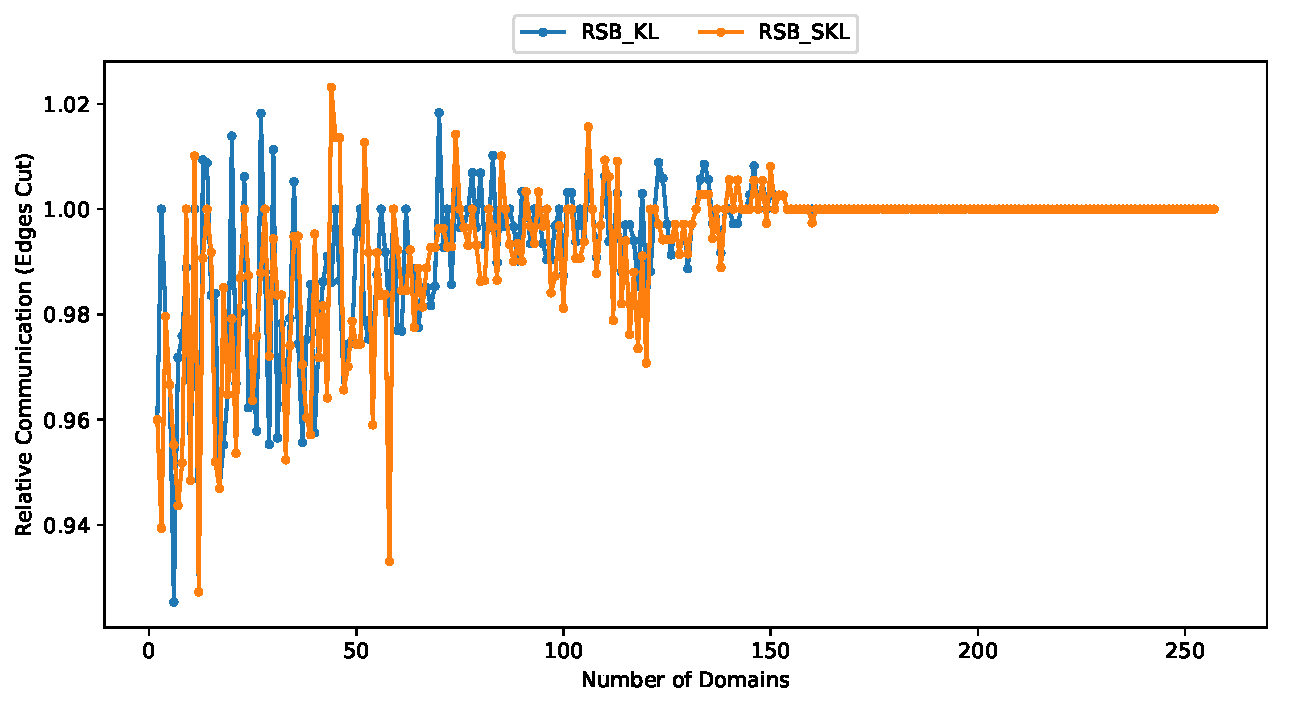
\includegraphics[width=\resultwidth]{results/2D/RSB_Edges_Cut_Relative}
        \caption{Communication relative to the \ac{RSB} method without refinement as a function of number of domains for each refinement method using the \ac{RSB} partitioning method.\label{fig:Spatial Decomposition:2D RSB Refinement}}
      \end{figure}

      \begin{figure}
        \centering
        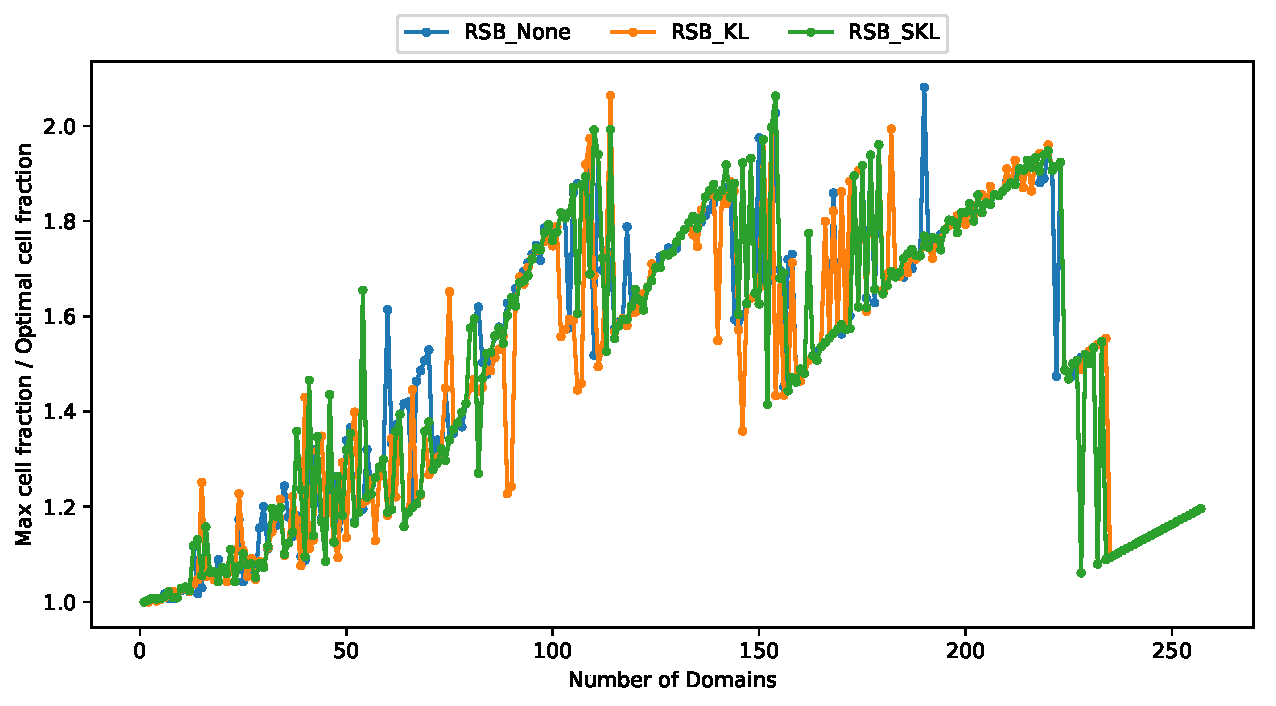
\includegraphics[width=\resultwidth]{results/2D/RSB_Size_to_Optimal}
        \caption{Ratio of maximum cell fraction to optimal cell fraction for the \ac{RSB} partitioning method with each refinement method. \label{fig:Spatial Decomposition:RSB Refinement Balance}}
      \end{figure}
    }
  }
  %%%%%%%%%%%%%%%%%%%%%%%%%%%%%%%%%%%%%%%%%%%%%%%%%%%%%%%%%%%%%%%%%%%%%%%%%%%%%%
  % Conclusions
  %%%%%%%%%%%%%%%%%%%%%%%%%%%%%%%%%%%%%%%%%%%%%%%%%%%%%%%%%%%%%%%%%%%%%%%%%%%%%%
  \section{Conclusions}{\label{sec:Spatial Decomposition:Conclusions}
    Spatial decomposition is a useful technique for reducing the runtime of simulations and is necessary to run whole-core high fidelity reactor calculations.
    Using graph partitioning methods to decompose the spatial domain of a core has significant advantages when compared to previous decomposition methods.
    Graph partitioning allows for the usage of an arbitrary number of spatial subdomains, and it generalizes to different module geometries such as a hexagonal lattice.
    Graph partitioning methods generally provide high quality decompositions that increase parallel efficiency.
    These automated spatial decomposition methods improve code usability and flexibility by allowing users to easily fit simulations to any number of processors.

    However, for highly decomposed cores, the convergence rate decreases due to jagged subdomain boundaries.
    This caused graph partitioning methods to significantly reduce runtime for problems that were not highly decomposed but actually increase runtime for highly decomposed problems.
    Additionally, the graph partitioning methods allow for an arbitrary number of domains to be used, unlike the previous method, giving the user significantly more options.
    This is because the assembly-based decomposition method used rectangular (non-jagged) subdomains.
    This indicates that it may be advantageous to create a high quality decomposition method that enforces rectangular subdomains.
    However, this approach will not generalize to other lattice types, such as hexagonal lattices.

    In the current MPACT implementation, there is no significant difference in run-times when using any of the three partitioning methods discussed, although \ac{REB} typically results in slightly lower \ac{MOC} run-times.
    The 2-D results indicate that the maximum fraction of cells in a subdomain is highly correlated with the runtime of the simulation.
    Furthermore, 2-D results indicate that the parallel efficiency of \ac{MOC} is highly correlated with the ratio of the optimal cell fraction per subdomain to the maximum cell fraction in a subdomain.

    In 3-D, MPACT currently requires spatial domains to be axially and radially aligned, for the 2D/1D method.
    If these restrictions are lifted, then other approaches can be used to perform the 3-D spatial decomposition.
    Three 3-D decomposition approaches were investigated in this work: radial and axial aligned subdomains, radially aligned subdomains, and an approach with no alignment restrictions.
    The radially aligned approach is expected to out perform the current approach by an average of 10\% for typical cases.
    However, the unrestricted approach is actually expected to perform worse than the current approach on average because the problem is well balanced axially.
    This analysis was performed on a 3-D core, which was relatively homogeneous in the axial direction; if a core design were to be more axially heterogeneous, then a more significant increase in performance might be expected.

    The parallel efficiency is a measure of how well computational resources are utilized in parallel applications.
    MPACT's overall parallel efficiency decreases rapidly as more domains are used due to two factors: increased number of iterations, and the inefficiency of the parallel \ac{CMFD} solve.
    For the 2-D VERA progression problem 5a, the overall parallel efficiency of MPACT dropped to nearly 20\%.
    The parallel efficiency of only the \ac{MOC} computations in MPACT drops to between 40--60\%, while the parallel efficiency of the \ac{CMFD} computation drops to $<\!\!20$\%.
    This causes the \ac{CMFD} computation to dominate runtime in spatially decomposed cases, and motivates the implementation of a more efficient parallel linear system operator in MPACT rather than using a third-party library.
  }

  % References
  \printbibliography
}
    \chapter{Improved Linear Source Formulation for Multi-physics and 2D/1D Applications}{
  \label{ch:Improved Linear Source Formulation for Multi-physics and 2D/1D Applications}
  %%% Multi-group Energy quantities %%%
\DeclareDocumentCommand{\gprime}{}{g^{\prime}}
% Cross-sections
\DeclareDocumentCommand{\xs}{ O{t} O{\loc} O{g}}{\ensuremath{\CrossSection_{#1}^{#3}(#2)}}
\DeclareDocumentCommand{\xst}{ O{\loc} O{g} }{\xs[t][#1][#2]}
\DeclareDocumentCommand{\xsa}{ O{\loc} O{g} }{\xs[a][#1][#2]}
\DeclareDocumentCommand{\xsf}{ O{\loc} O{\gprime} }{\xs[f][#1][#2]}
\DeclareDocumentCommand{\xss}{ o O{\loc} O{\dirprime\vdot\dir} O{\gprime \to g} }{
    \IfNoValueOrEmptyTF{#1}
    {\xs[s][#2,#3][#4]}
    {\xs[s,#1][#2][#4]}
}
\DeclareDocumentCommand{\spect}{ O{\loc} O{g} }{\ensuremath{\Spectrum^{#2}(#1)}}
\DeclareDocumentCommand{\nufis}{ O{\loc} O{\gprime} }{ \ensuremath{\nu\xsf[#1][#2]}}
\DeclareDocumentCommand{\D}{ O{\loc} O{g} }{\ensuremath{D^{#2}(#1)}}

% Flux
\DeclareDocumentCommand{\aflux}{ O{\loc} O{\dir} O{g} }{\ensuremath{\AngularFlux^{#3}(#1,#2)}}
\DeclareDocumentCommand{\sflux}{ O{\loc} O{\gprime} }{\ensuremath{\ScalarFlux^{#2}(#1)}}
\DeclareDocumentCommand{\current}{ O{\loc} O{g} }{\ensuremath{\Current^{#2}(#1)}}
\DeclareDocumentCommand{\fluxmoma}{ O{\ell} O{n} O{\loc} O{g} }{\ensuremath{\ScalarFlux^{#2,#4}_{#1}(#3)}}

% Source
\DeclareDocumentCommand{\source}{ O{\loc} O{\dir} O{g} }{\ensuremath{q^{#3}(#1,#2)}}
\DeclareDocumentCommand{\sourcemoma}{ O{\ell} O{n} O{\loc} O{g} }{\ensuremath{q^{#2,#4}_{#1}(#3)}}

  %%% Discrete Ordinates Quantities %%%
\DeclareDocumentCommand{\mprime}{}{m^{\prime}}
\DeclareDocumentCommand{\dirm}{ O{m} }{\dir_{#1}}
\DeclareDocumentCommand{\wt}{ O{m} }{\Weight_{#1}}

% Quadrature set
\DeclareDocumentCommand{\angquad}{ O{N} }{ \mathcal{M}_{#1} }

% Cross-Sections
\DeclareDocumentCommand{\xss}{ o O{\loc} O{ m^{\prime}\!\to m} O{\gprime\!\to g} }{
    \IfNoValueOrEmptyTF{#1}
    {\xs[s,#3][#2][#4]}
    {\xs[s,#1][#2][#4]}
}

% Flux
\DeclareDocumentCommand{\aflux}{ O{\loc} O{m} O{g}}{\ensuremath{\AngularFlux^{#3}_{#2}\!\left(#1\right)}}

% Source
\DeclareDocumentCommand{\source}{ O{\loc} O{m} O{g} }{\ensuremath{q^{#3}_{#2}\!\left(#1\right)}}

  %%% MOC quantities %%%
% Geometric
\DeclareDocumentCommand{\Length}{}{s}
\DeclareDocumentCommand{\NormalizedLength}{}{t}
\DeclareDocumentCommand{\len}{ O{} }{\Length_{#1}}
\DeclareDocumentCommand{\segl}{ O{mki} }{\Length_{#1}}
\DeclareDocumentCommand{\nlen}{ O{m} }{\NormalizedLength_{#1}}
\DeclareDocumentCommand{\nsegl}{ O{mki} }{\NormalizedLength_{#1}}

\DeclareDocumentCommand{\centroid}{ O{\loc} O{i} }{#1_{#2}^{\text{c}}}
\DeclareDocumentCommand{\locIn}{ O{\loc} O{mki} }{{#1}_{#2}^{\text{in}}}
\DeclareDocumentCommand{\locOut}{ O{\loc} O{mki} }{{#1}_{#2}^{\text{out}}}
\DeclareDocumentCommand{\locCent}{ O{\loc} O{mki} }{{#1}_{#2}^{\text{c}}}
\DeclareDocumentCommand{\M}{ o O{i}}{%
    \IfNoValueOrEmptyTF{#1}
        {\vec{M}_{#2}}
        {M_{#2,#1}}
}
\DeclareDocumentCommand{\C}{o O{i} O{g}}{%
    \IfNoValueOrEmptyTF{#1}
        {\vec{C}_{#2}^{#3}}
        {C_{#2,#1}^{#3}}
}


% Integration
\DeclareAutoPairedDelimiter{\MOCTrackIntegral}{\langle}{\rangle_{mki}}
\DeclareAutoPairedDelimiter{\MOCSingleAngleIntegral}{\langle}{\rangle_{mi}}
\DeclareAutoPairedDelimiter{\MOCIntegral}{\langle}{\rangle_{i}}

% Cross-sections
\DeclareDocumentCommand{\xs}{ O{t} O{i} O{g}}{\ensuremath{\CrossSection_{#1,#2}^{#3}}}
\DeclareDocumentCommand{\xst}{ O{i} O{g} }{\xs[t][#1][#2]}
\DeclareDocumentCommand{\xsa}{ O{i} O{g} }{\xs[a][#1][#2]}
\DeclareDocumentCommand{\xsf}{ O{i} O{\gprime} }{\xs[f][#1][#2]}
\DeclareDocumentCommand{\xss}{ o O{i} O{m'\to m} O{\gprime \to g} }{
    \IfNoValueOrEmptyTF{#1}
    {\xs[s][#2,#3][#4]}
    {\xs[s,#1][#2][#4]}
}

\DeclareDocumentCommand{\spect}{ O{i} O{g} }{\ensuremath{\Spectrum^{#2}_{#1}}}
\DeclareDocumentCommand{\nufis}{ O{i} O{\gprime} }{ \ensuremath{\nu\xsf[#1][#2]}}
\DeclareDocumentCommand{\D}{ O{i} O{g} }{\ensuremath{D^{#2}_{#1}}}
\DeclareDocumentCommand{\opt}{ O{m} O{g} }{\OpticalThickness_{#1}^{#2}}
\DeclareDocumentCommand{\segopt}{ O{mki} O{g} }{\opt[#1][#2]}

% MOC Parameters
\DeclareDocumentCommand{\tA}{ O{a} }{\ensuremath{\delta\!A_{#1}}}
\DeclareDocumentCommand{\Weight}{}{w}
\DeclareDocumentCommand{\wt}{ O{m} }{\Weight_{#1}}
\DeclareDocumentCommand{\wtbar}{ O{m} }{\overline{\Weight}_{#1}}
\DeclareDocumentCommand{\renorm}{ O{i} }{\ensuremath{\xi_{#1}}}

% Flux
\DeclareDocumentCommand{\aflux}{ O{mki} O{g} O{\len} }{
    \IfNoValueOrEmptyTF{#3}
    {\AngularFlux^{#2}_{#1}}
    {\ensuremath{\AngularFlux^{#2}_{#1}\!\left(#3\right)}}
}
\DeclareDocumentCommand{\afluxin}{ O{mki} O{g} }{\AngularFlux^{#2,\text{in}}_{#1}}
\DeclareDocumentCommand{\afluxout}{ O{mki} O{g} }{\AngularFlux^{#2,\text{out}}_{#1}}
\DeclareDocumentCommand{\sflux}{ O{g} O{i} }{\ScalarFlux_{#2}^{#1}}
\DeclareDocumentCommand{\current}{ O{i} O{g} }{\Current^{#2}_{#1}}
\DeclareDocumentCommand{\tfluxF}{ O{mki} O{g} }{ \overline{\AngularFlux}_{#1}^{#2} }          % Average flux-moment along track
\DeclareDocumentCommand{\tfluxL}{ O{mki} O{g} }{  \widehat{\AngularFlux}_{#1}^{#2} }          % Linear flux-moment along track
\DeclareDocumentCommand{\dflux}{ O{mki} O{g} }{ \Delta\AngularFlux_{#1}^{#2} }                % Difference of angular flux along track
\DeclareDocumentCommand{\sfluxF}{ O{i} O{g} }{ \overline{\ScalarFlux}_{#1}^{#2} }             % Average scalar flux
% \DeclareDocumentCommand{\sfluxL}{ o O{i} O{g} }{ % Linear expansion coeff (Scalar Flux)
%     \IfNoValueOrEmptyTF{#1}
%         {\lvec{\widehat{\ScalarFlux}}_{#2}^{#3}}
%         {\widehat{\ScalarFlux}_{#2,#1}^{#3}}
% }
\DeclareDocumentCommand{\sfluxL}{ O{i} O{g} o }{ % Linear expansion coeff (Scalar Flux)
    \IfNoValueOrEmptyTF{#3}
        {\lvec{\widehat{\ScalarFlux}}_{#1}^{#2}}
        {\widehat{\ScalarFlux}_{#1,#3}^{#2}}
}
% \DeclareDocumentCommand{\sfluxL}{ m O{i} O{g} }{\widehat{\ScalarFlux}_{#2,#1}^{#3} }          % Linear expansion coeff (Scalar flux)
\DeclareDocumentCommand{\afluxmom}{ O{\ell} O{n} O{i} O{\gprime} }{\FluxMoment_{#3,#1}^{#4,#2}}

% Source
\DeclareDocumentCommand{\source}{ O{mki} O{g} O{\len} }{\ensuremath{q^{#2}_{#1}\!\left(#3\right)}}
\DeclareDocumentCommand{\tsrcF}{ O{mki} O{g} }{ \overline{q}_{#1}^{#2} }          % Average source along track
\DeclareDocumentCommand{\tsrcL}{ O{mi} O{g} }{ \widehat{q}_{#1}^{#2} }          % Linear source along track
\DeclareDocumentCommand{\src}{ O{i} O{g} }{ \Source_{#1}^{#2}}                          % Generic source
\DeclareDocumentCommand{\srcF}{ O{i} O{g} }{ q_{#1}^{#2} }             % Average source
\DeclareDocumentCommand{\srcL}{ o O{i} O{g} }{ % Linear expansion coeff (Source)
    \IfNoValueOrEmptyTF{#1}
        {\lvec{\widehat{q}}_{#2}^{#3}}
        {\widehat{q}_{#2,#1}^{#3}}
}

% Linear source operators / functions
\DeclareDocumentCommand{\FluxToSource}{ O{g} }{\mathcal{S}^{#1}}
  \def\figpath{chapters/LSMOC/figures/}
  \graphicspath{ {\figpath} }

  \NewDocumentCommand{\modFunc}{}{\widehat{F}_2(\segopt)}

  The studies performed in this thesis have made extensive use of the \acf{LSA} introduced by \citet{Ferrer2016}.
  Through the use of the approximation, as presented in the original work, instabilities and inefficiencies were found.
  This chapter aims to present two improvements made to this approximation that have been a focus of this research: improved exponential tabulation \cite{Fitzgerald2018}, and an improved formulation for multi-physics and 2D/1D applications \cite{Fitzgerald2019}.

  %%%%%%%%%%%%%%%%%%%%%%%%%%%%%%%%%%%%%%%%%%%%%%%%%%%%%%%%%%%%%%%%%%%%%%%%%%%%%%
  % Exponential Tabulation
  %%%%%%%%%%%%%%%%%%%%%%%%%%%%%%%%%%%%%%%%%%%%%%%%%%%%%%%%%%%%%%%%%%%%%%%%%%%%%%
  \section{Exponential Tabulation}{\label{sec:LSMOC:Exponential Tabulation}
    The original moment-based \ac{LSMOC} formulation \cite{Ferrer2016}, detailed in \cref{sec:MOC:LSA}, uses several exponential functions:
    \begin{subequations}\label[subeqs]{eqs:LSMOC:ET:Exponential Functions}
      \begin{equation}\label{eq:LSMOC:ET:F1}
        F_1(\opt) \defined 1 - e^{\opt},
      \end{equation}
      \begin{equation}\label{eq:LSMOC:ET:F2}
        F_2(\opt) \defined 2\left[\opt - F_1(\opt)\right] - \segopt F_1(\opt),
      \end{equation}
      \begin{equation}\label{eq:LSMOC:ET:G1}
        G_1(\segopt) \defined 1 + \frac{\segopt}{2} - \left(1 + \frac{1}{\segopt}\right)F_1(\segopt),
      \end{equation}
      \begin{equation}\label{eq:LSMOC:ET:G2}
        G_2(\segopt) \defined \frac{2}{3}\segopt - \left(1 + \frac{2}{\segopt}\right)G_1(\segopt),
      \end{equation}
      and
      \begin{equation}\label{eq:LSMOC:ET:H}
        H(\segopt) \defined \frac{\segopt}{2} - G_1(\segopt),
      \end{equation}
    \end{subequations}
    where $\opt$ is the variable optical thickness, and $\segopt$ is the total optical thickness of a segment.
    Although the functions $F_1(\opt)$, and $F_2(\opt)$ are functions of variable $\opt$, in the implementation of this method in code they are only ever evaluated over the full optical thickness, $\segopt$.
    The functions, $G_1(\segopt)$, $G_2(\segopt)$, and $H(\segopt)$ all require special treatment around $\segopt = 0$, in this work this is handled via Taylor interpolation about $\segopt=0$.

    \begin{figure}
        \centering
        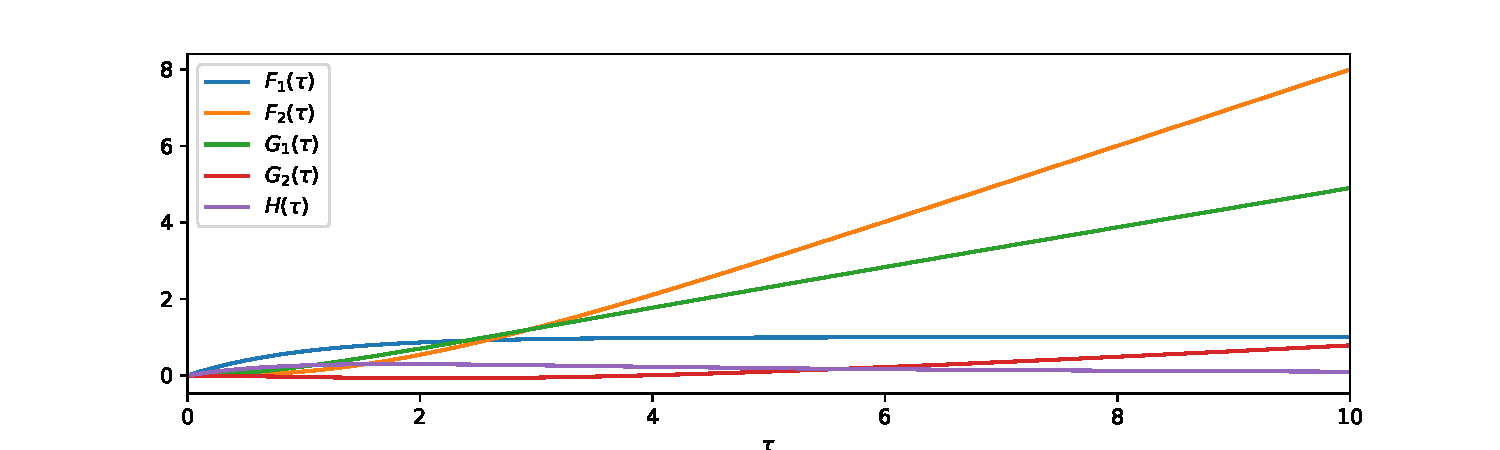
\includegraphics[width=0.90\linewidth]{exponentials/exponential-functions}
        \caption{The exponential functions, \cref{eqs:LSMOC:ET:Exponential Functions}, from 0 to 10.\label{fig:Exponential Functions}}
    \end{figure}

    These functions all involve an exponential, $e^{-\segopt}$; although this does not present a problem mathematically, the exponential function is a transcendental function that tends to be slow when evaluated computationally.
    For efficient transport codes, this presents a challenge.
    Previous works have demonstrated that function interpolation can provide significant run-time reduction \cite{Yamamoto2004}, and the original formulation \cite{Ferrer2016} suggested the use of function interpolation (though no details were provided).

    \subsection{First Approach: Improved Accuracy}{\label{ssec:LSMOC:ET:First Approach: Improved Accuracy}
      With the implementation of \ac{LSA} into MPACT, stability issues were observed in problems with very small transport cross sections, such as the fuel-clad gap in \acp{LWR}.
      These stability issues were only observed when exponential function interpolation was used, and the simplest method for addressing the issue was to increase the accuracy of the exponential interpolation.
      It was discovered that the root of the problem was the $F_2(\segopt)$ function in the transmission equation
      \begin{equation}\label{eq:LSMOC:ET:Transmission Original}
        \afluxout = \afluxin
                  + \left(\frac{\tsrcF}{\xst}-\afluxin\right)F_1(\segopt)
                  + \frac{\tsrcL}{2\left(\xst\right)^2}F_2(\segopt).
      \end{equation}
      In MPACT, source terms are actually computed and stored as $q/\xst$; however the $F_2(\segopt)$ term has an additional inverse $\xst$.
      In problems with near-void regions, where $\xst$ is small, any error in $F_2(\segopt)$ interpolation will be magnified.
      The simplest approach is to increase the accuracy of the exponential interpolation to account for the lowest expected cross sections; in the test problem this was on the order of $10^{-5}$.
      Thus, the expectation is that an interpolation 5 orders of magnitude more accurate than previous accuracy would be sufficient.
      Previous work \cite{Yamamoto2004} indicated that for \ac{FSMOC} calculations an max interpolation error of $10^{-7}$ was sufficient, i.e. for \ac{LSMOC} the max error would be within $10^{-12}$.

      Creating interpolation tables with the necessary accuracy for these problems requires some care.
      The original investigation of exponential interpolation for transport calculations  done by \citet{Yamamoto2004} indicated two methods of controlling interpolation accuracy.
      One method to increase interpolation accuracy is to increase the number of intervals (decreased interval width); however, this increased the memory.
      Alternatively, higher order polynomials can be used in the interpolation, which overall tends to reduce memory at the expense of increased run-times.

      In this investigation, two additional methods for controlling accuracy were investigated: interpolation node choice, and non-uniform interval widths.
      \subsubsection{Interpolation Points}{\label{sssec:ET:Interpolation Points}
        Within each interval of an interpolation table, the function is computed at interpolation points and an approximation of the function is made as the polynomial passing through these points.
        The placement of these points within each interval can greatly affect the accuracy of the approximation.
        Previous works \cite{Yamamoto2004,Kochunas2013} used evenly spaced interpolation points within each interval; however, this does not minimize the error in the approximation.
        An example is shown in \cref{fig:LSMOC:ET:Interpolation Example}.

        \begin{figure}
          \centering
          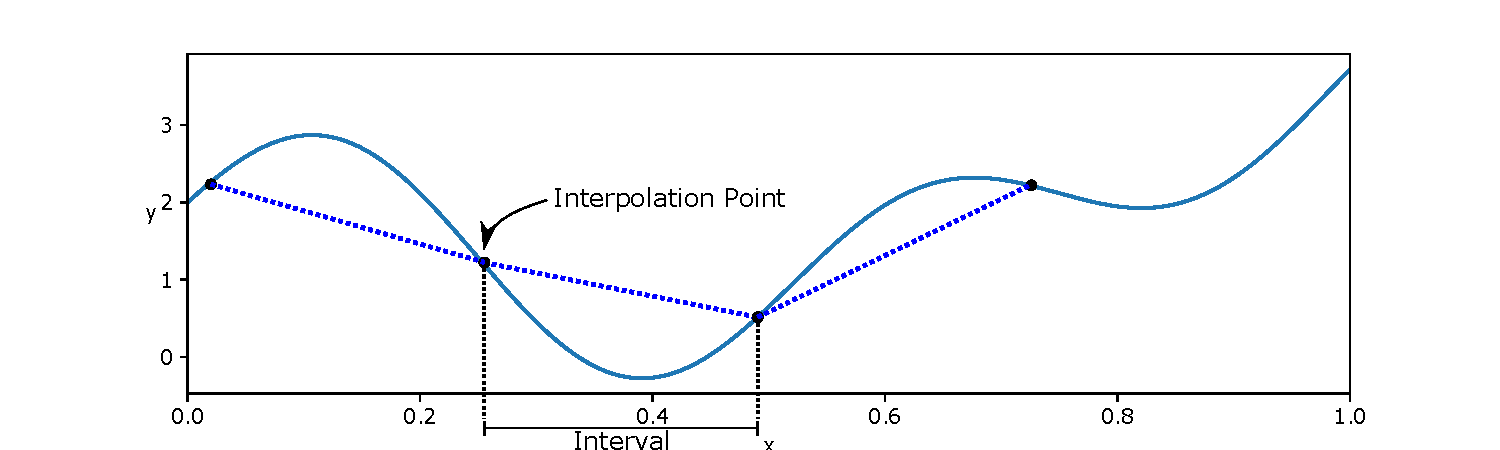
\includegraphics[width=0.90\linewidth]{exponentials/interpolation-example}
          \caption{Example of linear interpolation with uniform interval widths and interpolation points on the edge of the domain.\label{fig:LSMOC:ET:Interpolation Example}}
        \end{figure}

        Let $P_n(x)$ be the order $n$ polynomial approximating a function, $f(x)$, on an arbitrary interval $[a,b]$.
        The maximum error, $\epsilon$, within an interval is given by
        \begin{equation}\label{eq:LSMOC:ET:Interpolation Error}
          \epsilon = \frac{1}{(n+1)!}\left(\max_{\xi\in[a,b]}\lrabs{f^{(n+1)}(\xi)}\right)\left(\max_{x\in[a,b]}\lrabs{\prodl[j=1][n+1](x-x_j)}\right),
        \end{equation}
        for some value $\xi\in[a,b]$, where $f^{(n+1)}$ is the $n+1$-th derivative of $f(x)$.
        The choice of interpolation points will only affect the last term enclosed in parentheses.

        The Chebyshev points \cite{Stewart1996} are a set of values in $[a,b]$ that minimize $\max_{x\in[a,b]}\lrabs{\prodl[j=1][n+1](x-x_j)}$, and are given by
        \begin{equation}\label{eq:LSMOC:ET:Chebyshev Points}
          x_k = \frac{1}{2}\left[(a+b)+(b-1)\cos\left(\frac{2k-1}{2(n+1)}\pi\right)\right], \forall k\in\{1,2,...,n,n+1\}.
        \end{equation}
        By using the Chebyshev points, the maximum interpolation error, $\epsilon$, can be simplified to
        \begin{equation}\label{eq:LSMOC:ET:Chebyshev Interpolation Error}
          \epsilon = \frac{1}{2^n(n+1)!}\left(\frac{b-a}{2}\right)^{n+1}\max_{\xi\in[a,b]}\lrabs{f^{(n+1)}(\xi)}.
        \end{equation}
        Because the Chebyshev points do not include the end-points of the interval, there is additional cost in setting up the interpolation table, but this is negligible to typical \ac{MOC} calculation times.
        An interpolation table using Chebyshev points \emph{reduces error at no run-time cost} compared to a table using evenly spaced points.
        For this reason, Chebyshev points will be assumed for the remainder of this section.
        \Cref{tab:LSMOC:ET:Chebyshev Error} shows maximum errors for $F_1(\opt)$ interpolation for uniformly spaced points and Chebyshev points for an interval width $\Delta=b-a$.
        \begin{table}
          \centering
          \renewcommand{\arraystretch}{1.45}
          \caption{Maximum error in $F_1(\tau)$ for interval width $\Delta$.}
          \label{tab:LSMOC:ET:Chebyshev Error}
          \begin{tabular}{@{}ccc@{}}\toprule
            Polynomial Order & Uniform points   & Chebyshev points\\\midrule
            1                & $\frac{\Delta^2}{8}$           & $\frac{\Delta^2}{16}$\\
            2                & $\frac{\Delta^3}{72\sqrt{3}}$  & $\frac{\Delta^3}{192}$\\
            3                & $\frac{\Delta^4}{1536}$        & $\frac{\Delta^4}{3072}$\\\bottomrule
          \end{tabular}
        \end{table}
      }
      \subsubsection{Interval Width}{\label{sssec:LSMOC:ET:Interval Width}
        The conventional approach for interpolation tables has been to use a constant interval width, $\Delta$, for all intervals in the domain.
        This interval width is then used to control the error of the table.
        \Cref{eq:LSMOC:ET:Interpolation Error} shows that the interval bounds affect the interpolation error through the derivative term.
        The second and higher order derivatives of each of the exponential functions (\cref{eqs:LSMOC:ET:Exponential Functions}) approach zero as $\segopt$ approaches infinity.
        This indicates that the interpolation error typically decreases as the optical thickness increases in the conventional approach.

        However, is is possible to maintain the same maximum error over each interval if a variable interval width, $\Delta_i$, is used, where $i$ indicates the interval index.
        By using a variable interval width, a table can use fewer intervals while maintaining the same maximum error.
        However, since the widths are no longer constant, there is no longer a simple/direct conversion from $\segopt$ to $i$.
        Although there may be better ways, for this work the smallest interval is used to break up the domain into a map which points to the correct interval for that range of values.

        It was found that the use of non-uniform interval widths allowed for significantly fewer total intervals, reducing the memory usage, but incurring overhead for the additional mapping to index.
        \Cref{fig:LSMOC:ET:Memory Analysis} shows the memory usage for a polar-independent interpolation table for $F_1(\segopt)$.
        Using a non-uniform table typically decreases the memory usage by nearly an order of magnitude.
        For polar-dependent tables, the memory usage will be multiplied by the largest inverse sine of the polar angle, and the number of polar angles.

        \begin{figure}
          \centering
          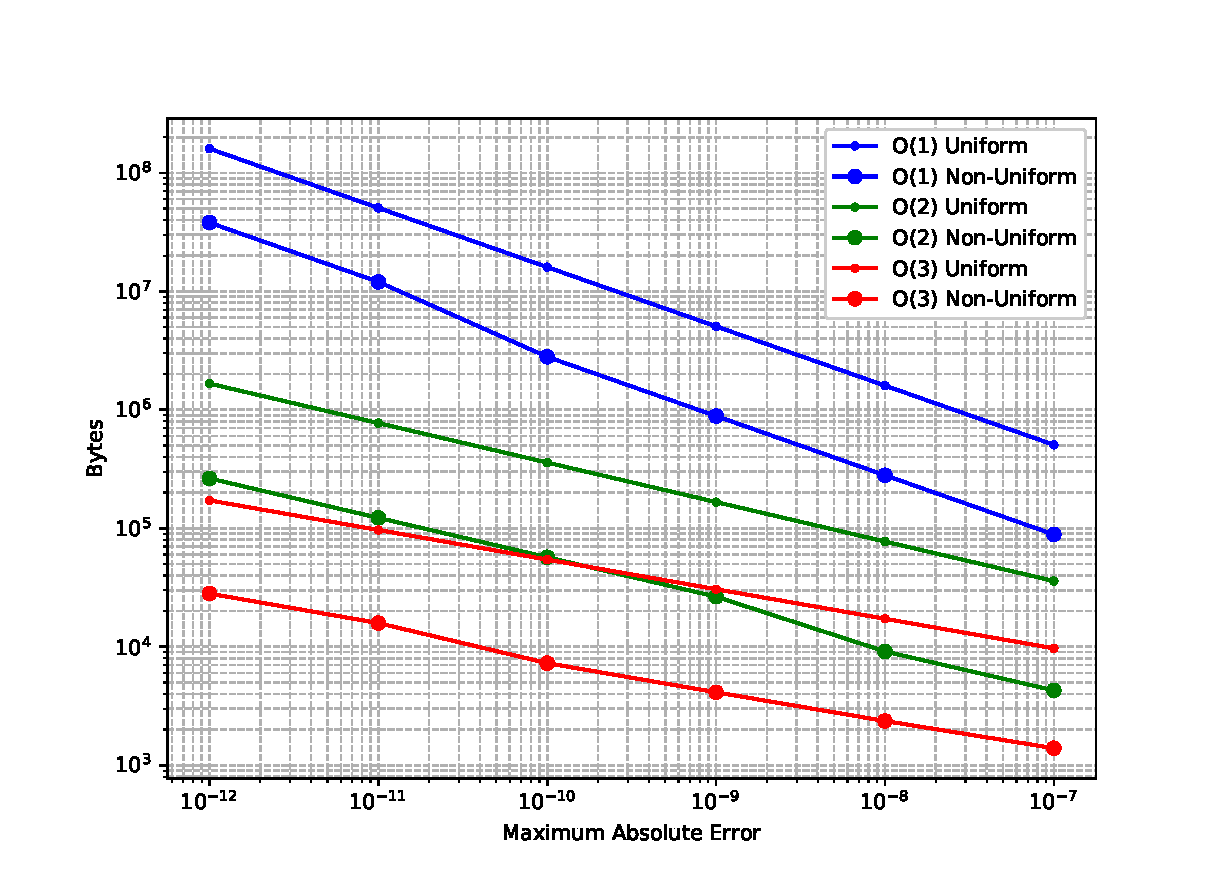
\includegraphics[width=0.90\linewidth]{exponentials/MemoryAnalysis}
          \caption{The memory usage of a single interpolation table (polar independent) for $F_1(\tau^g_{mki})$ is shown as a function of the maximum error for different interpolation orders and tabulation methods.\label{fig:LSMOC:ET:Memory Analysis}}
        \end{figure}

        Because all the functions of \cref{eqs:LSMOC:ET:Exponential Functions} are related, it is possible to tabulate only a single function and compute the others from the resulting interpolated value.
        However, if $F_1(\segopt)$ is known accurately, it is not possible to compute $H(\segopt)$ for very small $\segopt$ due to round-off errors.
        Instead one can tabulate $H(\segopt)$ and use the result to compute the other functions; however, this may incur more error than directly interpolating these functions.
      }
    }
    \subsection{Function Modification}{\label{ssec:LSMOC:ET:Function Modification}
      A second approach for addressing the instability due to inaccurate function interpolation was taken: change the functions.
      Recall that the highly accurate interpolation tables of \cref{ssec:LSMOC:ET:First Approach: Improved Accuracy} were necessary due to the inverse total (or transport) cross section on the $F_2(\segopt)$ term of \cref{eq:LSMOC:ET:Transmission Original}.
      Manipulating this term, we define a new function
      \begin{equation}\label{eq:LSMOC:ET:F2 Modified Definition}
        \frac{F_2(\segopt)}{\xst} = \nlen\modFunc,
      \end{equation}
      where
      \begin{equation}\label{eq:LSMOC:ET:F2 Modified}
        \modFunc \defined 2\left(1-\frac{F_1(\segopt)}{\segopt}\right) - F_1(\segopt).
      \end{equation}
      The $\modFunc$ function can be tabulated in place of $F_2(\segopt)$; this will require an additional multiplication by the segment length $\nsegl$ causing slight reduction in performance.
      But, by using the modified $\modFunc$ function, the underlying cause of the numerical instability is addressed, and the more accurate interpolation is no longer necessary.

      One approach is to tabulate the $\modFunc$ function in place of the $F_2(\segopt)$ function, and multiply by $\nsegl$ during evaluation.
      However, as stated in the previous section, it is possible to tabulate a single function and compute the others.
      The $H(\segopt)$ function could be tabulated again; but tabulating an intermediate function,
      \begin{equation}\label{eq:LSMOC:ET:E1}
        E_1(\segopt) \defined \frac{1-e^{-\segopt}}{\segopt},
      \end{equation}
      uses the same number of operations to compute the other functions.
      This $E_1(\segopt)$ function also has smaller derivative terms around $\segopt=0$, allowing for larger interval widths with no loss in accuracy.
      Therefore, it is expected that $E_1(\segopt)$ tabulation will be more efficient.
    }
    \subsection{Results}{\label{ssec:LSMOC:ET:Results}
      The results of this section were generated in serial on a Linux system with an Intel Xeon E3-1241 v3 (3.50 GHz) processors with 8 MB L3 cache.
      Results were generated for a 2-D \ac{MOC} transport calculation.
      In 2-D it is sometimes convenient to store separate interpolation tables for each polar angle.
      Both polar dependent and independent tables were tested.

      In both of the results sections, results were generated using tables for the three functions ($F_1(\segopt)$, $F_2(\segopt)$, $H(\segopt)$), or a single function (which is then used to compute the others).
      In the results, it is considered 3 functions, as the $G_1(\segopt)$, and $G_2(\segopt)$ functions are only used in pre-computing coefficients, and not in the main \ac{MOC} solver routine.

      \subsubsection{Results using More Accurate Tables}{\label{sssec:LSMOC:ET:Results using More Accurate Tables}
        \Cref{tab:LSMOC:ET:Naive Results} shows results for the different interpolation methods in a 2-D \ac{MOC} calculation.
        The use of non-uniform intervals significantly reduced the memory usage, but the run-times generally increased.
        This is likely due to the overhead from the additional index mapping operation; it is possible that a more efficient index mapping would change these results.

        The linear tables were significantly slower than higher-order interpolations, and the non-uniform linear tables were actually slower than just using the builtin transcendental functions.
        The poor performance is due to the main memory accesses caused by the table size exceeding the largest (L3) cache size.
        The polar independent tables were faster only in the case of the linear tables, due primarily to the reduction in memory.
        In all other cases the polar-dependent tables were able to more efficiently approximate the functions.
        Using either second or third order tables gave reasonably low run-times; compared to the analytic evaluations the order 2 uniform polar dependent table led to $\sim 3.5$x speed-up in the exponential time, and $\sim 1.9$x speed-up in the overall \ac{MOC} run-time.
        The results for both second and third order interpolation tables did not vary significantly, the second order was slightly faster for uniform tables.

        However, if a single function is tabulated and used to compute the others, the memory footprint of the interpolation tables can be significantly reduced.
        Moreover, the memory accesses are reduced in favor of floating point operations which increases the computational intensity and temporal cache locality of the implementation.
        Generally, this is a favorable strategy for improving code performance as a memory access is expected to take \emph{at minimum} the same time as a single \ac{FLOP}, with cache-misses increasing that time.
        Indeed, \cref{tab:LSMOC:ET:Naive Results} shows that tabulating the single function reduced run-time in all cases.

        \begin{table}
          \centering
          \caption{Results for different exponential function evaluation methods. Maximum interpolation error of $10^{-12}$. ``w/ pol'' indicates a table with polar dependence, and ``w/o pol'' indicates a table without polar dependence.}
          \label{tab:LSMOC:ET:Naive Results}
          \footnotesize
          \begin{tabular}{@{}ccrrrrrrrrr@{}}\toprule
            Method & Table Type & Order & \multicolumn{2}{c}{\shortstack[c]{Exponential\\Time (s)}} & & \multicolumn{2}{c}{\ac{MOC} Time (s)} && \multicolumn{2}{c}{Intervals (Memory)}\\\cmidrule{4-5}\cmidrule{7-8}\cmidrule{10-11}
                  &            &       & w/ pol & w/o pol & \phantom{}                           & w/ pol & w/o pol & \phantom{}  &  \multicolumn{1}{c}{w/ pol} & \multicolumn{1}{c}{w/o pol}\\\midrule
            Analytic & N/A & N/A & \multicolumn{2}{c}{432.5} && \multicolumn{2}{c}{654.7} && \multicolumn{2}{c}{N/A}\\\midrule
            \multirow{6}{*}{3-Functions}     & \multirow{3}{*}{Uniform}        & 1 & 382.6 & 360.3 && 622.5 & 591.0 && 6.00E7 (8.04 GB) & 1.00E7 (458 MB) \\\addlinespace[-0.2em]
                                                                              && 2 & 121.3 & 151.7 && 343.2 & 372.1 && 416080 (85.7 MB) & 69360  (4.8 MB) \\\addlinespace[-0.2em]
                                                                              && 3 & 124.1 & 169.0 && 347.5 & 388.7 && 32280  (9079 KB) & 5400   (506 KB) \\\cmidrule{2-11}\addlinespace[-0.2em]
                                                & \multirow{3}{*}{Non-Uniform} & 1 & 592.9 & 559.2 && 825.8 & 800.6 && 4.07E6  (878 MB) & 840658 (76.6 MB)\\\addlinespace[-0.2em]
                                                                              && 2 & 144.6 & 178.5 && 364.3 & 397.8 && 45265  (10.9 MB) & 8020    (835 KB)\\\addlinespace[-0.2em]
                                                                              && 3 & 139.6 & 199.8 && 358.5 & 420.0 && 4491    (1.4 MB) & 796    (85.2 KB)\\\midrule
            \multirow{6}{*}{1-Function}       & \multirow{3}{*}{Uniform}       & 1 & 296.2 & 259.3 && 523.9 & 484.5 && 6.00E7 (2.68 GB) & 1.00E7  (153 MB)\\\addlinespace[-0.2em]
                                                                              && 2 &  91.4 & 123.2 && 310.2 & 345.7 && 416080 (28.6 MB) & 69360  (1.59 MB)\\\addlinespace[-0.2em]
                                                                              && 3 &  87.2 & 133.2 && 305.4 & 353.6 && 32280  (2.96 MB) & 5400    (169 KB)\\\cmidrule{2-11}\addlinespace[-0.2em]
                                                & \multirow{3}{*}{Non-Uniform} & 1 & 474.6 & 424.0 && 714.6 & 653.9 && 4.07E6  (415 MB) & 722899 (49.2 MB)\\\addlinespace[-0.2em]
                                                                              && 2 & 105.8 & 146.4 && 326.6 & 367.7 && 41444   (4.4 MB) & 7338   (443  KB)\\\addlinespace[-0.2em]
                                                                              && 3 &  98.9 & 153.3 && 318.8 & 373.2 && 4152    (515 KB) & 735    (33.5 KB)\\\bottomrule
          \end{tabular}
        \end{table}
      }
      \subsubsection{Results using Modified Function}{\label{sssec:LSMOC:ET:Results using Modified Function}
        Results were generated for the same cases as the more accurate table, but the interpolation accuracy was $10^{-7}$ rather than $10^{-12}$, as the function modification addressed the cause of the instability.
        The results are summarized in \cref{tab:LSMOC:ET:Final Results}.
        In one approach the three functions are tabulated, in the other $E_1(\segopt)$ is tabulated and used to compute the three functions.
        Previous results showed that the polar-independent and non-uniform interval width tables were slower than uniform polar-dependent tables; here the results are only shown for the uniform polar-dependent interpolation tables.

        The interpolation accuracy is not required to be as high as in the previous cases, thus the tables are significantly smaller in memory size.
        The linear tables no longer exceed the L3 cache size and are not prohibitively slow to use.
        In fact, the linear tables are the fastest option for both 3-table and single-table interpolation methods.
        Interpolating $E_1(\segopt)$ and computing the other functions from the result was the fastest approach overall.
        As before, this is expected because this method favors \acp{FLOP} over memory accesses.

        This approach also significantly reduces the number of intervals necessary (by about 3 orders of magnitude).
        Although the higher-order interpolation ended up not being more efficient than the linear interpolation tables, the number of intervals is extremely small.
        These methods may be useful on different architectures (such as \acp{GPGPU}\footnote{this statement was not confirmed as part of this study, and is speculation based on knowledge of architecture constraints.}) where memory is more limited than on a single-threaded \ac{CPU} calculation.

        \begin{table}
          \centering
          \caption{Results using the modified function, with maximum interpolation error of $10^{-7}$. Memory is under 1 MB in all cases.}
          \label{tab:LSMOC:ET:Final Results}
          \begin{tabular}{@{}ccccc@{}}\toprule
            Method & Order & Exp.     & \ac{MOC}& \# Intervals \\
                   &       & Time (s) & Time (s) & \\\midrule
            \multirow{3}{*}{3-Functions}      & 1 &  88.4 & 307.9 & 4774\\
                                              & 2 &  99.7 & 316.8 &  225\\
                                              & 3 & 116.5 & 333.1 &   46\\\midrule
            \multirow{3}{*}{$E_1(\opt)$ Only} & 1 &  80.5 & 299.0 & 2739\\
                                              & 2 &  87.6 & 307.3 &  158\\
                                              & 3 &  99.0 & 317.7 &   38\\\bottomrule
          \end{tabular}
        \end{table}
      }
    }
    %%%%%%%%%%%%%%%%%%%%%%%%%%%%%%%%%%%%%%%%%%%%%%%%%%%%%%%%%%%%%%%%%%%%%%%%%%%%
    % Conclusions
    %%%%%%%%%%%%%%%%%%%%%%%%%%%%%%%%%%%%%%%%%%%%%%%%%%%%%%%%%%%%%%%%%%%%%%%%%%%%
    \subsection{Conclusions}{\label{ssec:LSMOC:ET:Conclusions}
      This study focused on the investigation of efficient approximation of the exponential functions in the \ac{LSMOC}.
      Methods for efficiently approximating the exponential function for \ac{FSMOC} have previously been investigated.
      However, these methods, applied without modification to the \ac{LSMOC} can lead to numerical instability in problems with near-void regions.
      One approach to deal with these instabilities is to improve the accuracy of the interpolation tables based on the lowest cross section in the problem.
      While this approach can be made efficient, if cross sections become too small the tables may become exceedingly large and significantly hamper performance.

      This investigation revealed that the cause of the instability was the $F_2(\segopt)$ function in the transmission equation.
      By instead manipulating the term including this function, the cause of the instabilities can be addressed.
      This approach no longer requires excessively large interpolation tables; however, some key-findings from the first approach can be applied to make this approach faster.
      First, the use of Chebyshev points significantly increases interpolation accuracy for the same number of intervals as uniformly spaced points, at no run-time cost.
      Additionally, by interpolating a single function and using the result to compute the other functions performance can be significantly improved.
    }
  }
  %%%%%%%%%%%%%%%%%%%%%%%%%%%%%%%%%%%%%%%%%%%%%%%%%%%%%%%%%%%%%%%%%%%%%%%%%%%%%%
  % Improved Linear Source Formulation for Multi-physics and 2D/1D Applications
  %%%%%%%%%%%%%%%%%%%%%%%%%%%%%%%%%%%%%%%%%%%%%%%%%%%%%%%%%%%%%%%%%%%%%%%%%%%%%%
  \section{Improved Linear Source Formulation for Multi-physics and 2D/1D Applications}{\label{sec:Improved Linear Source Formulation for Multi-physics and 2D/1D Applications}
    As stated in \cref{sec:MOC:LSA}, the original derivation of the moment-based \acf{LSA} from \citet{Ferrer2016} faced inefficiencies in problems with non-constant cross sections.
    The inefficiencies arose from the use of pre-computed coefficients, \cref{eq:MOC:LSA:C Matrix}, which must be re-computed if cross sections change.
    In multiphysics calculations, such as with \ac{TH} feedback, cross sections typically change each iteration, leading to significant overhead from re-computing these terms.
    This section presents and equivalent formulation, which eliminates the need to re-compute these terms if cross sections change, without additional operations.

    \subsection{Derivation}{\label{ssec:LSMOC:Derivation}
      The derivation of this improved formulation begins with the same initial steps as the derivation detailed in \cref{ssec:MOC:LSA:Derivation}.
      Several of these equations are repeated in this section for clarity.
      The source is assumed to have a spatially linear shape
      \begin{equation}\label{eq:LSMOC:Source Shape}
        \source[mi][g][\loc] \approx \srcF[mi] + \loc\vdot\srcL[][mi],
      \end{equation}
      and the angular flux moments can be expanded similarly
      \begin{equation}\label{eq:LSMOC:Flux Expansion}
        \fluxA(\loc) = \fluxF + \loc\vdot\fluxL.
      \end{equation}
      The source can be computed from the flux moments using \cref{eq:MOC:LSA:Linear Source Computation}.

      Computing the source requires the flux to be evaluated during transport sweeping.
      The angular flux moments are given by \cref{eqs:MOC:LSA:Region-Averaged Flux Moments Definitions}, but are repeated here for clarity.
      \begin{subequations}\label[subeqs]{eqs:LSMOC:Region-Averaged Flux Moments Definitions}
        The spatially flat angular flux moments are defined by integrating the flux multiplied by a spherical harmonics moment function over space and directions,
        \begin{equation}\label{eq:LSMOC:Region-Averaged Flux Moment Definition}
            \fluxF \defined \MOCIntegral{\SH \aflux[][g][]} = \frac{\fourpi}{V_i}\suml[m]\wt\SH[\ell][n][\dirm]\suml[k]\tA[mki]\nsegl\MOCTrackIntegral{\aflux[][g][]}.
        \end{equation}
        To determine the spatial expansion coefficients of the flux moments, \cref{eq:LSMOC:Flux Expansion} is operated on by $\MOCIntegral{\SH\loc(\vdot)}$.
        As before, this should be directly proportional to the angular flux operated on by $\MOCIntegral{\SH\loc\aflux[][g][]}$, a system of equations is found
        \begin{equation}\label{eq:LSMOC:Moment to Expansion Coefficient}
            \M\fluxL = \MOCIntegral{\SH\loc\aflux[][g][]},
        \end{equation}
        where
        \begin{equation}\label{eq:LSMOC:Geometric Moments}
            \M \defined \MOCIntegral{\loc^T\loc}.
        \end{equation}
        The spatial angular flux moments, $\MOCIntegral{\SH\loc\aflux[][g][]}$, are then defined as
        \begin{equation}\label{eq:LSMOC:Region-Averaged Spatial Angular Flux Moments Definition}
            \MOCIntegral{\SH\loc\aflux[][g][]} = \frac{\fourpi}{V_i}\suml[m]\wt\SH[\ell][n][\dirm]\suml[k]\tA[mki]\nsegl\left(\locIn\MOCTrackIntegral{\aflux[][g][]} + \dirm\MOCTrackIntegral{\nlen\aflux[][g][]} / \renorm[mi]\right).
        \end{equation}
      \end{subequations}

      With the assumed source shape, \cref{eq:LSMOC:Source Shape}, the characteristic transport equation becomes
      \begin{subequations}\label[subeqs]{eqs:LSMOC:Characteristic Form}
        The characteristic transport equation becomes
        \begin{equation}\label{eq:LSMOC:Characteristic Form}
          \left[\deriv{}{\nlen} + \xst\right]\aflux = \tsrcF + \tsrcL\left(\nlen - \frac{\nsegl}{2}\right),
        \end{equation}
        where
        \begin{equation}\label{eq:LSMOC:Track Average Source}
          \tsrcF \defined \rfourpi\left[\srcF[mi] + \locCent \vdot \srcL[][mi]\right],
        \end{equation}
        \begin{equation}\label{eq:LSMOC:Track Linear Source}
          \tsrcL \defined \rfourpi\left[\frac{\dirm\vdot\srcL[][mi]}{\renorm[mi]}\right],
        \end{equation}
        and $\locCent$ is the local-coordinate centroid of the track-segment.
      \end{subequations}
      Substituting this assumed source shape (linear) into the generic \ac{MOC} solution, given by \cref{eq:MOC:MOC Generic Solution}, the angular flux along a track-segment is found to be
      \begin{subequations}\label[subeqs]{eqs:LSMOC:Angular Flux Solution}
          \begin{equation}\label{eq:LSMOC:Angular Flux Solution}
              \aflux = \afluxin + \left(\frac{\tsrcF}{\xst} - \afluxin\right)F_1(\opt) + \frac{\tsrcL}{2(\xst)^2}F_2(\opt),
          \end{equation}
          where
          \begin{equation}\label{eq:LSMOC:F1}
              F_1(\opt) \defined 1 - \exp(-\opt),
          \end{equation}
          and
          \begin{equation}\label{eq:LSMOC:F2}
              F_2(\opt) \defined 2[\opt-F_1(\opt)] - \segopt F_1(\opt).
          \end{equation}
      \end{subequations}

      To evaluate the moments defined in \cref{eqs:LSMOC:Region-Averaged Flux Moments Definitions}, the track-average flux and first spatial moment of the angular flux must be determined.
      \begin{subequations}\label[subeqs]{eqs:LSMOC:Flux Track Moments}
        The track-average flux is determined as it was before, by operating on \cref{eq:LSMOC:Characteristic Form} by $\nsegl\MOCTrackIntegral{(\vdot)}$, yielding
        \begin{equation}\label{eq:LSMOC:0th Track Moment of the Flux}
          \MOCTrackIntegral{\aflux[][g][]} = \frac{\tsrcF}{\xst} + \frac{\dflux}{\segopt}.
        \end{equation}
        At this point the two derivations diverge from one another.
        In the previous formulation, the integral in $\MOCTrackIntegral{\nlen\aflux[][g][]}$ is \emph{explicitly} evaluated by substituting in the solution of the angular flux along the track (\cref{eqs:MOC:LSA:Angular Flux Solution}).
        Here, the moment will be found implicitly by operating on \cref{eq:LSMOC:Characteristic Form} by $\nsegl\MOCTrackIntegral{\nlen(\vdot)}$, just as was done for the 0th moment.
        This results in
        \begin{equation}\label{eq:LSMOC:1st Track Moment of the Flux}
          \MOCTrackIntegral{\nlen\aflux[][g][]} =
            \frac{\MOCTrackIntegral{\aflux[][g][]} - \afluxout}{\xst}
              + \frac{\nsegl}{2}\left[\frac{\tsrcF}{\xst}
              + \frac{\tsrcL}{\xst}\frac{\nsegl}{6}\right].
        \end{equation}
        Unlike \cref{eq:MOC:LSA:Track-Averaged Linear Angular Flux}, there a not any new exponential functions introduced in this form.
      \end{subequations}

      Previously, the average track flux, $\MOCTrackIntegral{\aflux[][g][]}$, was expanded to find a simpler final form.
      This is the case here as well; however, the out-going flux, $\afluxout$, will not be expanded, as this must necessarily be computed during transmission.
      \Cref{eqs:LSMOC:Region-Averaged Flux Moments Definitions} can be simplified into
      \begin{subequations}\label[subeqs]{eqs:LSMOC:Region-Averaged Flux Moments}
        \begin{equation}\label{eq:LSMOC:Region-Averaged Flat Flux Moments}
          \fluxF = \frac{\fourpi}{V_i\xst}\suml[m]\wt\SH\suml[k]\tA\left(\nsegl\tsrcF + \dflux\right),
        \end{equation}
        and
        \begin{aequation}\label{eq:LSMOC:Region-Averaged Linear Flux Moments}
          \MOCIntegral{\SH\loc\aflux[][g][]}
            = &\frac{1}{V_i}\suml[m]\wt\SH\suml[k]\tA\nsegl\left[\locCent\srcF + \left(\locCent(\locCent)^T + \frac{\segl^2}{12}\dirm\dirm^T\right)\srcL\right]\\
            + &\frac{\fourpi}{V_i\xst}\suml[m]\wt\SH\suml[k]\tA\left[\locIn\dflux + \dirm\segl\left(\frac{\dflux}{\segopt}-\afluxout+\frac{\tsrcF}{\xst}\right)\right]
        \end{aequation}
      \end{subequations}

      \Cref{eq:LSMOC:Region-Averaged Linear Flux Moments} contains $\dflux/\segopt$ terms, rather than only $\dflux$ terms.
      For numerical stability, it is beneficial to compute this quantity directly, rather than $\dflux$ and performing division.
      This can be found by evaluating the transmission equation, \cref{eq:LSMOC:Angular Flux Solution}, giving
      \begin{subequations}\label[subeqs]{eqs:LSMOC:Average Slope}
        \begin{equation}\label{eq:LSMOC:Average Slope}
          \frac{\dflux}{\segopt} = \left(\afluxin-\frac{\tsrcF}{\xst}\right)E_1(\segopt) - \frac{\nsegl}{2}\frac{\tsrcL}{\xst}T_2(\segopt),
            \end{equation}
            where
            \begin{equation}\label{eq:LSMOC:E1}
                E_1(\segopt) \defined \frac{F_1(\segopt)}{\segopt},
            \end{equation}
            \begin{equation}\label{eq:LSMOC:T2}
                T_2(\segopt) \defined 2E_2(\segopt) - E_1(\segopt),
            \end{equation}
            and
            \begin{equation}\label{eq:LSMOC:E2}
                E_2(\segopt) \defined \frac{1-E_1(\segopt)}{\segopt}.
            \end{equation}
      \end{subequations}
      Here, $E_2(\segopt)$ is defined as an intermediate function which has smaller derivative terms, meaning higher accuracy with fewer interpolation intervals (see \cref{sec:LSMOC:Exponential Tabulation}).
      Following the conclusions of \cref{sec:LSMOC:Exponential Tabulation}, only the $E_2(\segopt)$ function needs to be tabulated, and then is used to compute the other two exponential functions, $E_1(\segopt)$, and $T_2(\segopt)$.
      The outgoing flux can then be evaluated as
      \begin{equation}\label{eq:LSMOC:Outgoing Flux}
        \afluxout = \afluxin - \segopt\frac{\dflux}{\segopt}.
      \end{equation}
    }
    \subsection{Particle Conservation}{\label{ssec:LSMOC:Particle Conservation}
      As described in \cref{ssec:MOC:LSA:Particle Conservation}, particle conservation puts the constraint of using direction-dependent renormalization and centroids, in addition to directional quadrature constraints.
      If these constraints are satisfied, \cref{eqs:LSMOC:Region-Averaged Flux Moments} can be simplified into
      \begin{subequations}\label[subeqs]{eqs:LSMOC:Conservation:Region-Averaged Flux Moments}
        \begin{equation}\label{eq:LSMOC:Conservation:Region-Averaged Flat Flux Moments}
          \fluxF = \suml[m]\wt\SH\frac{\srcF}{\xst} + \frac{\fourpi}{V_i\xst}\suml[m]\wt\SH\suml[k]\tA\dflux,
        \end{equation}
        and
        \begin{aequation}\label{eq:LSMOC:Conservation:Region-Averaged Linear Flux Moments}
          \MOCIntegral{\SH\loc\aflux[][g][]} =
            &\suml[m]\wt\SH\M[][mi]\frac{\srcL}{\xst}\\
            +& \frac{\fourpi}{V_i\xst}\suml[m]\wt\SH\suml[k]\tA\left[\locIn\dflux + \dirm\segl\left(\frac{\dflux}{\segopt}-\afluxout+\frac{\tsrcF}{\xst}\right)\right],
        \end{aequation}
        where
        \begin{equation}\label{eq:LSMOC:Direction-Dependent M}
          \M[][mi] \defined \frac{1}{V_i}\suml[k]\tA\left[\locCent(\locCent)^T+\frac{\segl^2}{12}\dirm\dirm^T\right].
        \end{equation}
      \end{subequations}

      Although the above form seems to more computationally efficient, it would be negligent for this chapter to not include a more mathematically elegant form of \cref{eq:LSMOC:Region-Averaged Linear Flux Moments}.
      The terms in the second summation may be rewritten as
      \begin{subequations}\label[subeqs]{eqs:LSMOC:Region-Averaged Linear Flux Moments Elegant}
        \begin{aequation}\label{eq:LSMOC:Region-Averaged Linear Flux Moments Elegant}
          \MOCIntegral{\SH\loc\aflux[][g][]} =&
            \suml[m]\wt\SH\M[][mi]\frac{\srcL}{\xst} \\
            &+ \frac{\fourpi}{V_i}\suml[m]\wt\SH\suml[k]\tA\left[\locIn\left(\afluxin-\tfluxF\right)-\locOut\left(\afluxout-\tfluxF\right)\right],
        \end{aequation}
        where $\tfluxF$ is the average track flux,
        \begin{equation}\label{eq:Average Track Flux}
          \tfluxF \defined \nsegl\MOCTrackIntegral{\aflux[][g][]}.
        \end{equation}
      \end{subequations}
      In this form, the interior summation over track-segments becomes a spatially weighted summation of the incident and outlet flux differences from the average flux.
    }
    \subsection{Isotropic Simplifications}{\label{ssec:LSMOC:Isotropic Simplifications}
      If the so called \acf{LIFA} scheme is used, the spatially flat moment equations do not change; however, \cref{eq:LSMOC:Region-Averaged Linear Flux Moments} can be simplified to
      \begin{aequation}\label{eq:LSMOC:LIFA:Region-Averaged Linear Flux Moments}
        \MOCIntegral{\SH\loc\aflux[][g][]} &= \M\frac{\srcL}{\xst}\\ &+ \frac{\fourpi}{V_i\xst}\suml[m]\wt\suml[k]\tA\left[\locIn\dflux+\dirm\segl\left(\frac{\dflux}{\segopt}-\afluxout+\frac{\tsrcF}{\xst}\right)\right]
      \end{aequation}
    }
  }

  \section{Results}{\label{sec:LSMOC:Results}
    This section highlights several of the key results found using the \ac{LSA} solver implemented in MPACT.
    Only results using 2-D transport or the 2D/1D method in MPACT are shown, as 3-D transport results will be discussed in [REF].
    Isotopic depletion is performed using the ORIGEN code, and \ac{TH} feedback is performed using \ac{CTF}.
    Although \cref{sec:Improved Linear Source Formulation for Multi-physics and 2D/1D Applications} provides the derivation of a spatially linear anisotropic source, the initial implementation in MPACT was limited to the isotropic scattering approximation.
    With the use of the \ac{TCP0} approximation, problems of interest are able to be simulated with acceptable levels of error.
    However, one of our recent works \cite{Herring2020} has implemented the \ac{LIFA} approximation in MPACT, but these results are not presented here.

    \subsection{C5G7 Benchmark}{\label{ssec:LSMOC:C5G7 Benchmark}
      The 2-D C5G7 benchmark \cite{Smith2006} is a neutronics benchmark used by various codes to help verify the correctness of the solvers used.
      A 7-group cross section library of macroscopic cross sections is provided by the benchmark.
      The benchmark consists of two \ac{UO2} assemblies and two \ac{MOX} assemblies surrounded by a large radial reflector, as shown in \cref{fig:LSMOC:C5G7:CoreGeom}.
      Reflective boundary conditions are used on the north and west faces, while vacuum conditions are used on the south and east faces.
      The benchmark provides reference MCNP calculation results, which can be used to determine the accuracy of the methods used to solve the benchmark cases.

      \begin{figure}[htbp]
        \centering
        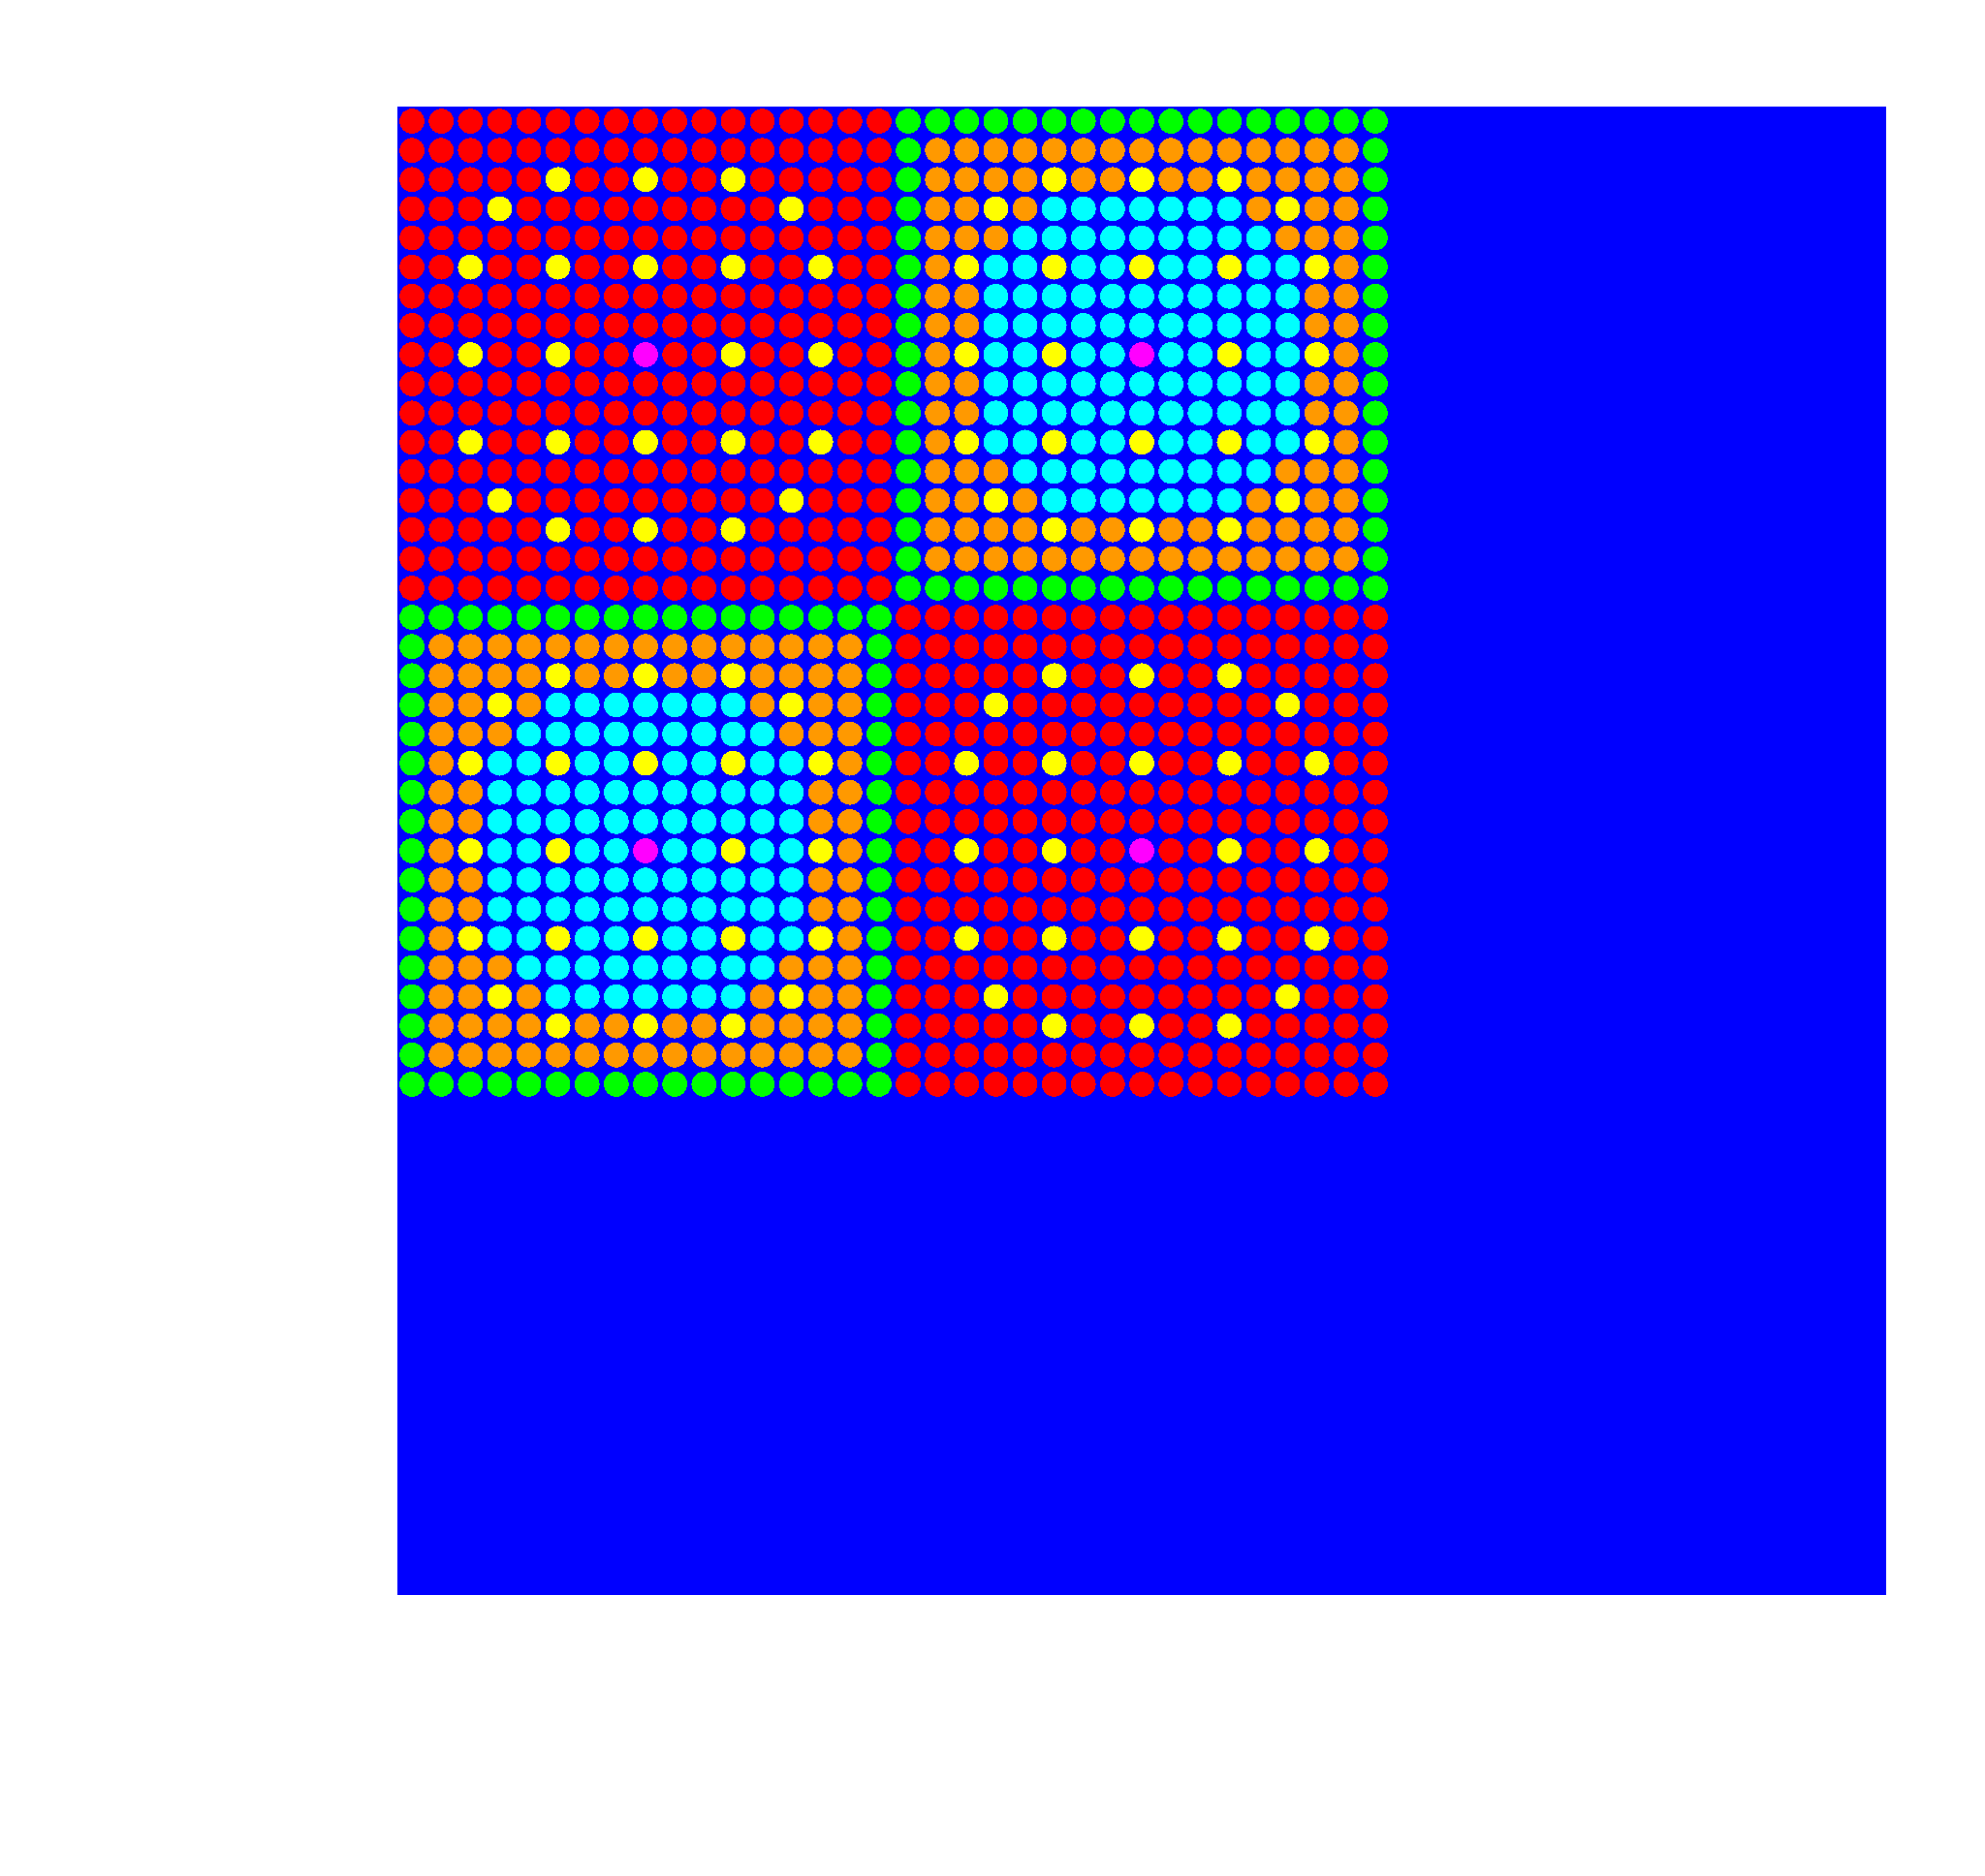
\includegraphics[width=0.45\linewidth]{\figpath/c5g7/core}
        \caption{Geometry and materials of the 2-D C5G7 benchmark. \label{fig:LSMOC:C5G7:CoreGeom}}
      \end{figure}

      This problem was studied in order to verify that the implementation of the \ac{LSA} derived in this chapter yields similar results to those found by \citet{Ferrer2016}.
      Similar meshing, ray, and direction parameters were used in this study as were used in the original study \cite{Ferrer2016}; some parameters could not be replicated exactly due to differences in the MPACT and CASMO5 codes.
      All cases used a uniform ray-spacing of 0.05 cm, and directional quadrature using 128 azimuthal angles and 6 polar angles in $\fourpi$.
      Each case was run using od\ac{CMFD} \cite{Zhu2016}.

      The fine pin cell mesh used 5 rings in the fuel region, 10 in the moderator region, and 16 azimuthal divisions in all regions.
      The fine reflector cell mesh was divided into 0.105$\times$0.105 cm$^2$ cells.
      The coarse pin cell mesh used a single fuel ring with four azimuthal divisions, and no moderator rings, using 8 azimuthal divisions in the surrounding moderator.
      The coarse reflector cell mesh was divided into 0.42$\times$0.42 cm$^2$ cells.

      Three cases were run in this study: fine mesh with \ac{FSA}, coarse mesh with \ac{FSA}, and coarse mesh with \ac{LSA}.
      To be consistent with \citet{Ferrer2016} results, it is expected that the \ac{LSA} on the coarse mesh should reduce run-time while maintaining accuracy compared to the finely mesh \ac{FSA} calculation.
      Additionally, the coarse mesh \ac{FSA} calculation should have significantly worse accuracy, thus justifying the use of the \ac{LSA}.

      \Cref{tab:LSMOC:C5G7:Results} shows very clearly that the \ac{LSA} on the coarse mesh is more accurate than the \ac{FSA} on the fine mesh.
      While \ac{FSA} on the fine mesh provides reasonable accuracy, the \ac{FSA} on the coarse mesh shows significant errors compared to the MCNP reference.
      In terms of accuracy, the results agree very closely with those reported for the original derivation of the moment-based \ac{LSA}.
      The reference pin-powers are visualized in \cref{figs:LSMOC:C5G7:Reference:PinPowers}, and the differences are shown in \cref{figs:LSMOC:C5G7:FineFS:PinPowers,figs:LSMOC:C5G7:CoarseFS:PinPowers,figs:LSMOC:C5G7:CoarseLS:PinPowers}.
      The largest pin-power differences for the fine mesh with \ac{FS} and coarse mesh with \ac{LS} are in the center assembly where pin-powers are higher.
      Interestingly, the largest pin-power differences for the coarse mesh with \ac{FS} case are in the pins bordering the radial reflector region;
        this indicates that the mesh in the reflector was not sufficient.
      Errors in the interior of the assemblies are still larger for this case than the others.

      \Cref{tab:LSMOC:C5G7:Performance} indicates that the \ac{LSA} on the coarse mesh significantly out performs the \ac{FSA} on the fine mesh;
      \ac{MOC} run-time is reduced by approximately 50\%, and memory usage is reduced by 45\%.
      However, this also shows that for this problem the \ac{LSA} solver takes just under 2 times the time of the \ac{FSA} on the same mesh (coarse).
      It is also shown, that there is very little memory overhead from using the \ac{LSA} on the same mesh as the \ac{FSA}.
      The number of iterations is quite different of that reported by \citet{Ferrer2016}; however, the iteration scheme in CASMO5 is different than that of MPACT \cite{FerrerPersoanlCommunications2018}.
      In MPACT, each iteration loops over all energy groups a single time, but in CASMO5 the thermal energy groups are iterated over multiple times.

      \begin{table}[htbp]
        \centering
        \caption{
          Accuracy comparisons for the C5G7 2-D benchmark calculation using different source approximations and meshes.
          In addition to eigenvalue difference, several metrics for comparing pin-powers are provided.
          The abbreviations are as follows:
            MPP+ = difference in maximum pin-power, MPP- = difference in minimum pin-power,
            AVE = average pin-power error, RMS = root-mean-square pin-power error,
            MRE = mean relative error.
          The number of pins with power within 68\% and 95\% of the MCNP reference results are also listed.
        }
        \label{tab:LSMOC:C5G7:Results}
        \begin{tabular}{rrrrrrrrrrr}\toprule
                 &      &                     & \multicolumn{6}{c}{Pin Powers (\%)} & \multicolumn{2}{c}{\# Pins within}\\
          Solver & Mesh & $\Delta\keff$ (pcm) & MPP+ & MPP- & MPE & AVE & RMS & MRE & 68\% & 95\%\\\midrule
          FSA    & Fine    & 8                & -0.13 & 0.89 & 0.98 & 0.18 & 0.24 & 0.15 & 494 & 763\\
          FSA    & Coarse  & 65               & -0.76 & 3.74 & 4.23 & 0.78 & 1.16 & 0.61 & 142 & 217\\
          LSA    & Coarse  & 2                &  0.02 & 0.30 & 0.66 & 0.12 & 0.16 & 0.10 & 663 & 901\\\bottomrule
        \end{tabular}
      \end{table}

      \begin{table}[htbp]
        \centering
        \caption{Performance comparisons for the C5G7 2-D benchmark calculation using different source approximations and meshes.}
        \label{tab:LSMOC:C5G7:Performance}
        \begin{tabular}{rrrrrr}\toprule
                 &      &            & \multicolumn{2}{c}{Run-time (s)} & \\\cline{4-5}
          Solver & Mesh & Iterations & MoC & MoC / iter   & Memory (MB)\\\midrule
          FSA    & Fine   & 13         & 435 & 33         & 409\\
          FSA    & Coarse & 11         &  89 &  8         & 213\\
          LSA    & Coarse & 13         & 209 & 16         & 223\\\bottomrule
        \end{tabular}
      \end{table}

      \begin{figure}[htbp]
        \centering
        \begin{subfigure}[t]{0.49\textwidth}
          \centering
          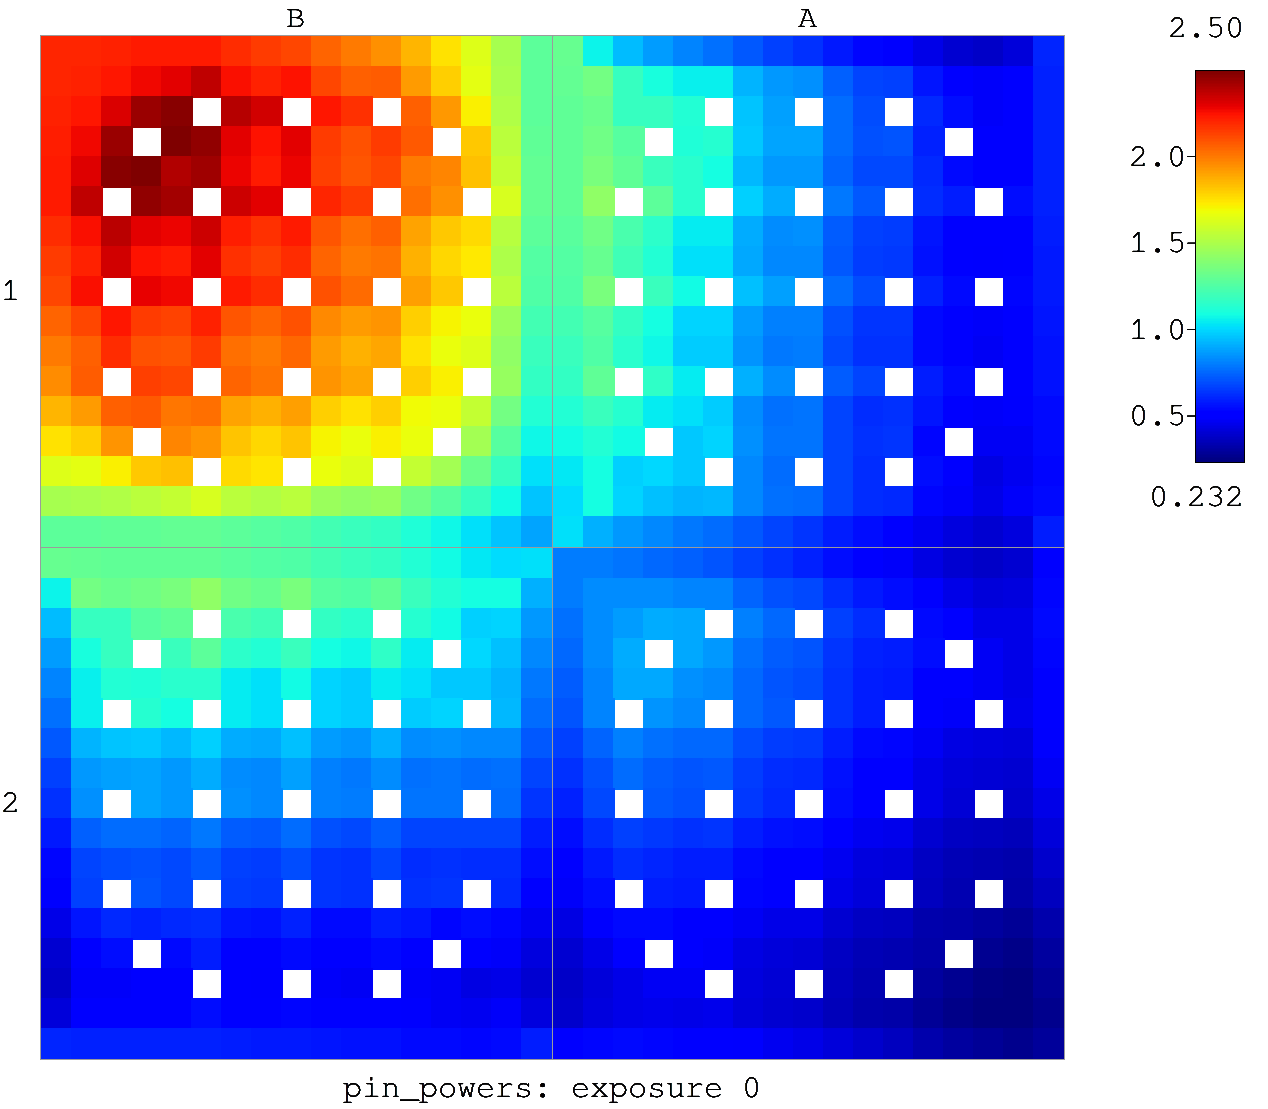
\includegraphics[width=\textwidth]{\figpath/c5g7/PinPowersCore}
          \caption{core \label{fig:LSMOC:C5G7:Reference:PinPowers:Core}}
        \end{subfigure}%
        ~
        \begin{subfigure}[t]{0.49\textwidth}
          \centering
            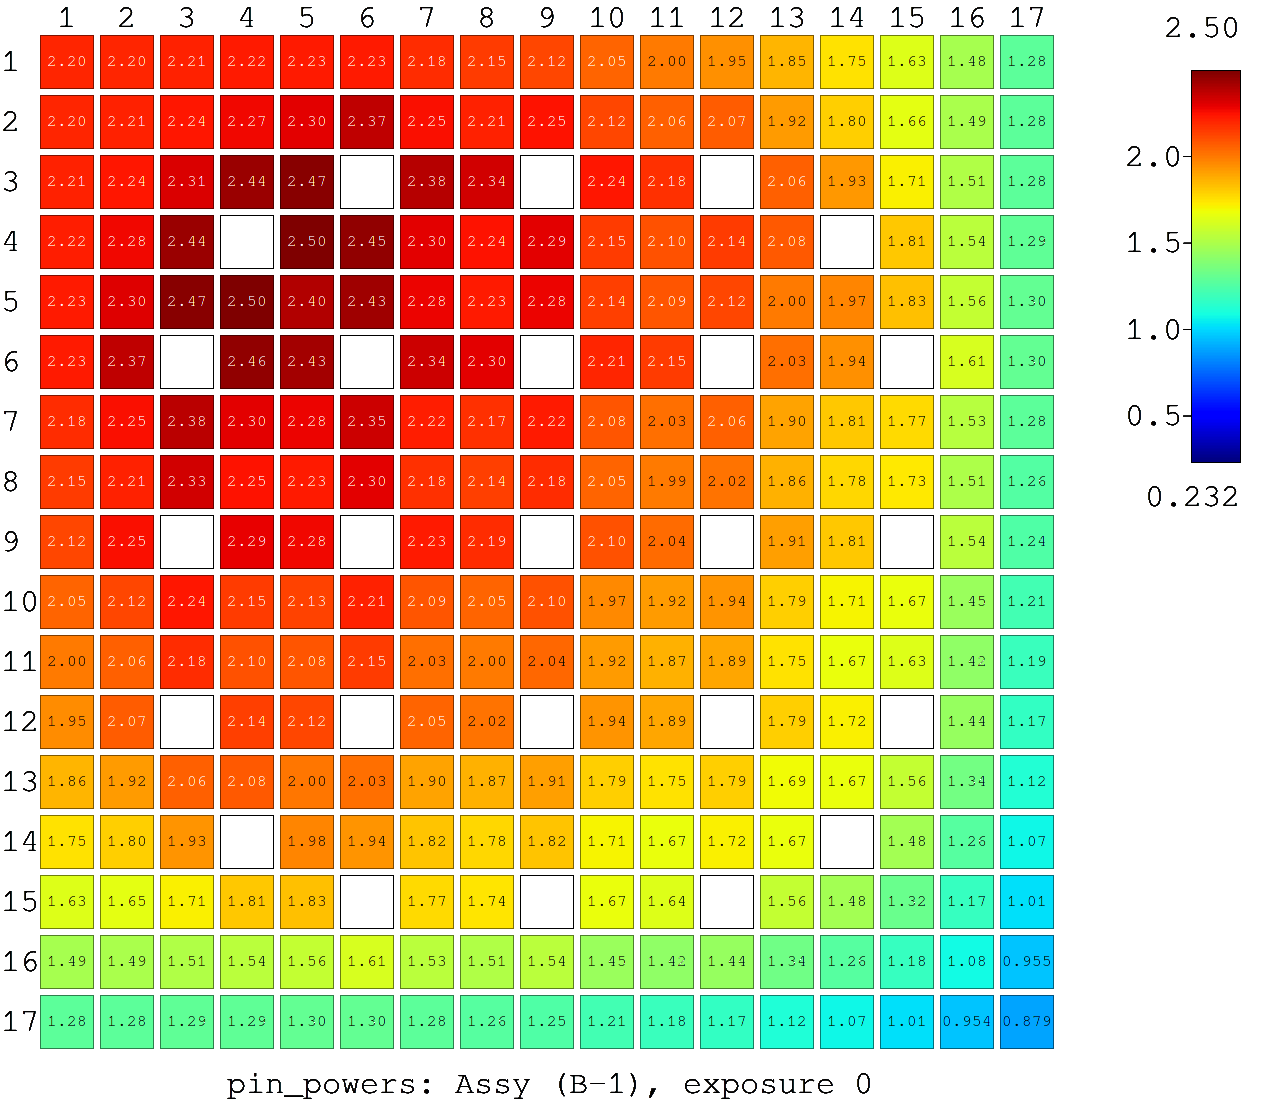
\includegraphics[width=\textwidth]{\figpath/c5g7/PinPowersAssembly}
            \caption{center assembly\label{fig:LSMOC:C5G7:Reference:PinPowers:Assembly}}
        \end{subfigure}
        \caption{Reference pin powers shown for the core and center assembly.\label{figs:LSMOC:C5G7:Reference:PinPowers}}
      \end{figure}
      \begin{figure}[htbp]
        \centering
        \begin{subfigure}[t]{0.49\textwidth}
          \centering
          \includegraphics[width=\textwidth]{\figpath/c5g7/fineFS/DiffPinPowersCore}
          \caption{core\label{fig:LSMOC:C5G7:FineFS:PinPowers:Core}}
        \end{subfigure}%
        ~
        \begin{subfigure}[t]{0.49\textwidth}
          \centering
            \includegraphics[width=\textwidth]{\figpath/c5g7/fineFS/DiffPinPowersAssembly}
            \caption{center assembly\label{fig:LSMOC:C5G7:FineFS:PinPowers:Assembly}}
        \end{subfigure}
        \caption{Pin power differences from reference shown for the core and center assembly for the fine mesh using the FSA solver.\label{figs:LSMOC:C5G7:FineFS:PinPowers}}
      \end{figure}
      \begin{figure}[htbp]
        \centering
        \begin{subfigure}[t]{0.49\textwidth}
          \centering
          \includegraphics[width=\textwidth]{\figpath/c5g7/coarseFS/DiffPinPowersCore}
          \caption{core\label{fig:LSMOC:C5G7:CoarseFS:PinPowers:Core}}
        \end{subfigure}%
        ~
        \begin{subfigure}[t]{0.49\textwidth}
          \centering
            \includegraphics[width=\textwidth]{\figpath/c5g7/coarseFS/DiffPinPowersAssembly}
            \caption{center assembly\label{fig:LSMOC:C5G7:CoarseFS:PinPowers:Assembly}}
        \end{subfigure}
        \caption{Pin power differences from reference shown for the core and center assembly for the coarse mesh using the FSA solver.\label{figs:LSMOC:C5G7:CoarseFS:PinPowers}}
      \end{figure}
      \begin{figure}[htbp]
        \centering
        \begin{subfigure}[t]{0.49\textwidth}
          \centering
          \includegraphics[width=\textwidth]{\figpath/c5g7/coarseLS/DiffPinPowersCore}
          \caption{core\label{fig:LSMOC:C5G7:CoarseLS:PinPowers:Core}}
        \end{subfigure}%
        ~
        \begin{subfigure}[t]{0.49\textwidth}
          \centering
            \includegraphics[width=\textwidth]{\figpath/c5g7/coarseLS/DiffPinPowersAssembly}
            \caption{center assembly\label{fig:LSMOC:C5G7:CoarseLS:PinPowers:Assembly}}
        \end{subfigure}
        \caption{Pin power differences from reference shown for the core and center assembly for the coarse mesh using the LSA solver.\label{figs:LSMOC:C5G7:CoarseLS:PinPowers}}
      \end{figure}
    }

    \subsection{Typical Pin Cell Depletion}{\label{ssec:LSMOC:Typical Pin Cell Depletion}
      In order to evaluate the benefits of this new formulation, the first multiphysics case studied was a typical \ac{UO2} fuel cell, as specified by \ac{VERA} progression problem 1A \cite{VERAProblems}.
      Isotopic depletion calculations were run up to 70 \ac{GWDMT} ($\sim$1820 \ac{EFPD}) at \ac{HFP} conditions.
      Using the current default meshing parameters in MPACT as a starting point, various mesh parameters were coarsened to study their affect when using the \ac{LSMOC}.
      These cases were compared against a reference case which was very finely meshed with fine ray-spacing (0.001 cm), and a Tabuchi-Yamamoto \cite{Yamamoto2005} quadrature using 128 azimuthal angles and 4 polar angles over $\fourpi$
      All other cases were run using a Tabuchi-Yamamoto quadrature with 64 azimuthal angles and 4 polar angles, with a uniform ray-spacing of 0.05 cm.
      This case used the \ac{TCP0} approximation to scattering.

      \paragraph{Default Mesh}{
        MPACT's current default meshing parameters were used as a starting point.
        Flat and linear source calculations were run on this mesh, to set a baseline for ``acceptable'' levels of error in the eigenvalue.
        Compared to the reference case, the \ac{LS} calculation had a larger maximum error in eigenvalue of 89.2 \ac{pcm}, whereas the \ac{FS} calculation had a maximum error of 65.5 \ac{pcm}.
        However, the average errors over the depletion were approximately the same: 31.6 and 33.7 \ac{pcm}, for the \ac{FS} and \ac{LS} calculations, respectively.
        The eigenvalue differences over the depletion calculation are shown in \cref{fig:LSMOC:1a:DefaultMesh:Eigenvalue}.
        The goal in this mesh refinement study is to determine acceptable meshing parameters without worse maximum or average eigenvalue errors.

        \begin{figure}
            \centering
            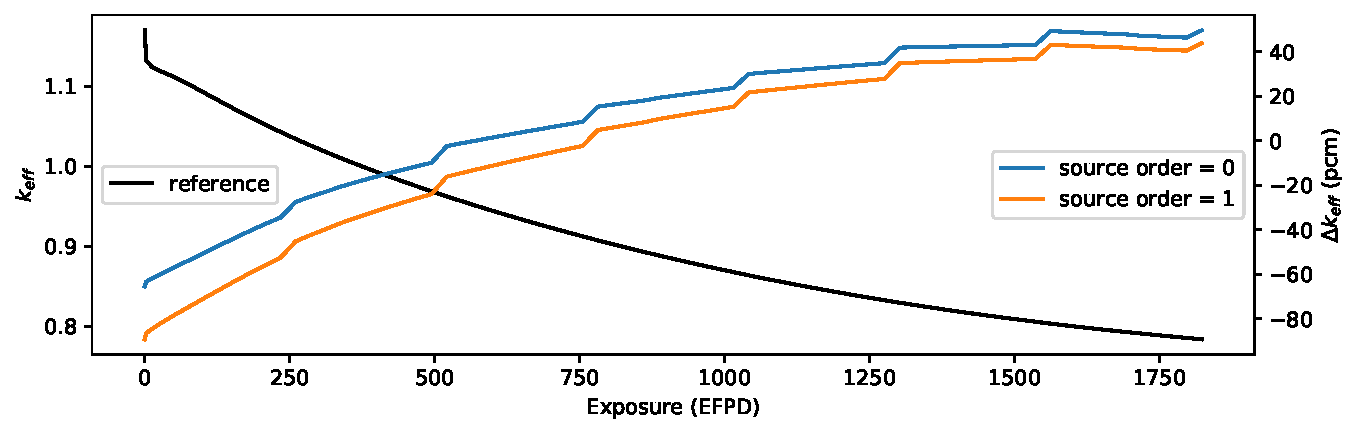
\includegraphics[width=\linewidth]{1a/DefaultMesh-Eigenvalues}
            \caption{Reference eigenvalues and differences for the default mesh pin cell case with isotopic depletion. \label{fig:LSMOC:1a:DefaultMesh:Eigenvalue}}
        \end{figure}
      }
      \paragraph{Fuel Radius}{
        During isotopic depletion, it is important to accurately capture the radial distribution of Plutonium, due to self-shielding effects.
        Plutonium is primarily produced in the outer rim of the pin, this is well known as the rim-effect.
        The default mesh uses three equal volume rings in the fuel region; however, we expect that two rings will be sufficient, when using the \ac{LSA}, if the extra ring is placed in such a way that it captures this rim-effect.
        Experimental studies of the rim-effect \cite{Lassmann1994} have found that there is a sharp rise in Plutonium at around between 80-90\% of the outer radius of the fuel.

        A series of calculations were run using two fuel rings with varying inner radius.
        The eigenvalue and Plutonium comparisons are shown in \cref{fig:LSMOC:1a:FuelRadius:Eigenvalue,fig:LSMOC:1a:FuelRadius:Pu239}.
        Comparing eigenvalues, a fractional radius between 0.825 and 0.875 seem to have little effect on the mean or worst-case eigenvalue difference.
        By comparing the concentration of Pu-239, these radii are again shown to be the most accurate; a fractional radius of 0.875 was chosen to be sufficient, and used in the remainder of the studies.

        \begin{figure}
            \centering
            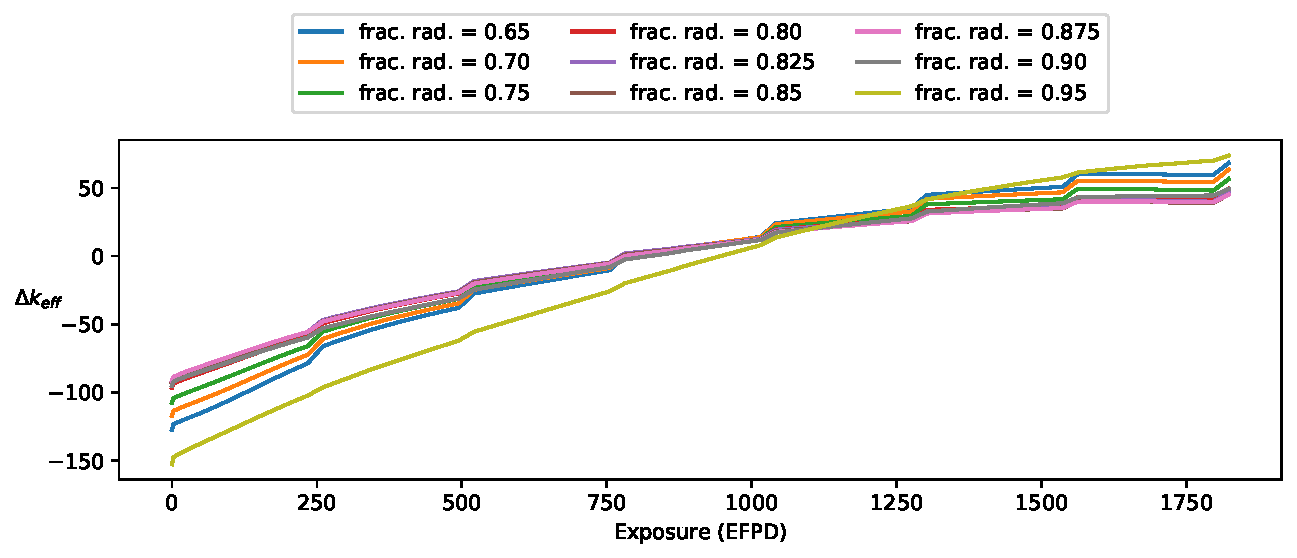
\includegraphics[width=\linewidth]{1a/FuelRadius-Eigenvalues}
            \caption{Eigenvalue comparisons for problem 1A using various inner fuel radii. \label{fig:LSMOC:1a:FuelRadius:Eigenvalue}}
        \end{figure}
        \begin{figure}
          \centering
          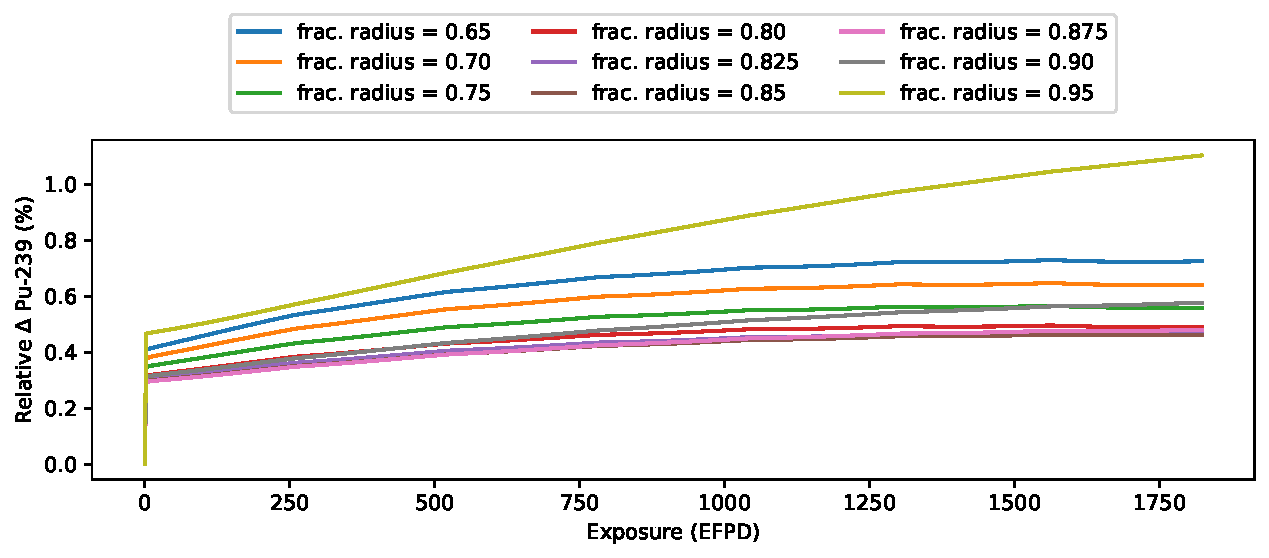
\includegraphics[width=\linewidth]{1a/FuelRadius-Pu239}
          \caption{Pu-239 concentration comparisons for problem 1A using various inner fuel radii. \label{fig:LSMOC:1a:FuelRadius:Pu239}}
        \end{figure}
      }
      \paragraph{Moderator Ring and Azimuthal Divisions} {
        The remaining mesh parameters are the azimuthal divisions in the fuel, clad, gap, and moderator regions, and the presence of an additional surrounding ring of moderator.
        While it may be sufficient to use a single azimuthal division in some regions in larger cases, due to symmetry of this single pin case, using a single azimuthal region would cause the linear components of the source to be zero (i.e. it is equivalent to the \ac{FSA}).
        It was found that the coarsening of these parameters have an insignificant affect on the resulting eigenvalue when using the \ac{LSA}, with less than 1 \ac{pcm} difference over the entire depletion.
        Thus, four azimuthal divisions in each material region, and no additional surrounding moderator ring was found to be sufficiently accurate in this case.
      }
      The coarse default and coarse meshes are displayed in \cref{figs:LSMOC:1A:Mesh}.

      \begin{figure}[h]
          \centering
          \begin{subfigure}[t]{0.45\textwidth}
              \centering
              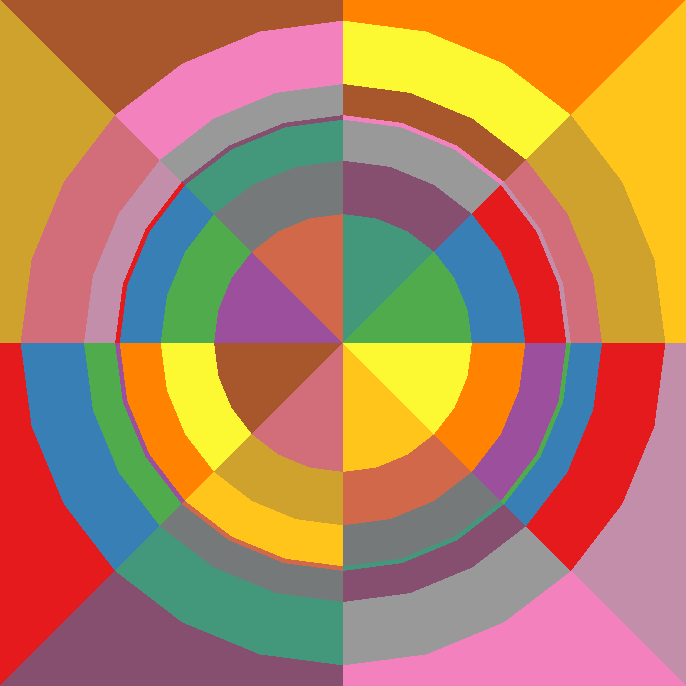
\includegraphics[width=0.9\textwidth]{1a/1a-default-trimmed}
              \caption{default mesh\label{fig:LSMOC:1a:Default Mesh}}
          \end{subfigure}%
          ~
          \begin{subfigure}[t]{0.45\textwidth}
              \centering
              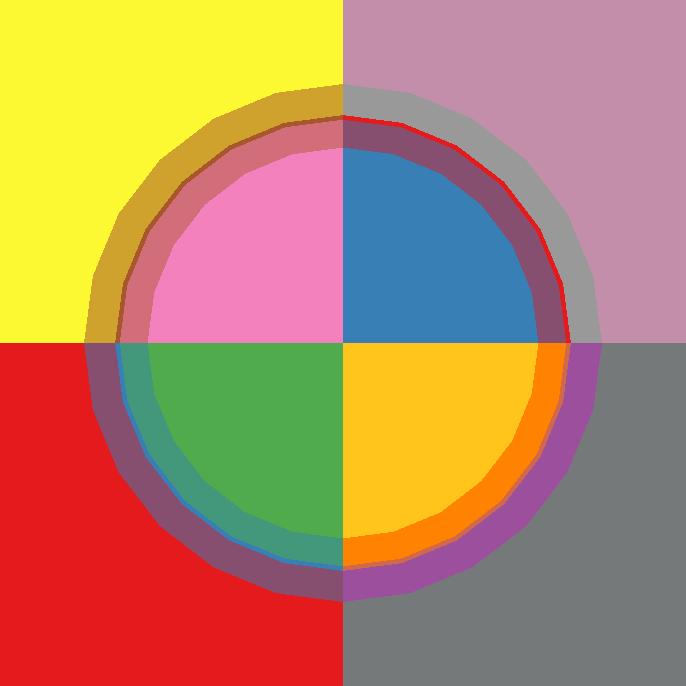
\includegraphics[width=0.9\textwidth]{1a/1a-coarse-trimmed}
              \caption{coarse mesh\label{fig:LSMOC:1a:Coarse Mesh}}
          \end{subfigure}
          \caption{VERA problem 1A (a) default and (b) coarse meshes.\label{figs:LSMOC:1A:Mesh}}
      \end{figure}
    }

    \subsection{VERA Problem 2A and 2P Depletion}{\label{ssec:LSMOC:VERA Problem 2A and 2P Depletion}
      A mesh study similar to that done in \cref{ssec:LSMOC:Typical Pin Cell Depletion} was performed on modified \ac{VERA} problems 2A and 2P \cite{VERAProblems} with isotopic depletion up to 70 \ac{GWDMT}.
      This was done to verify that the meshing parameters previously found were valid for larger problems, and determine if even coarser parameters were sufficient.
      First, problem 2A was studied; the meshing parameters of the fuel cell and guide-tube cells were studied independently.
      Both problems were simulated using the \ac{TCP0} scattering approximation.
      \subsubsection{Problem 2A}{\label{sssec:LSMOC:Problem 2A}
        \paragraph{2A - Default Mesh}{
          For this problem, a reference calculation was carried out on the lattice with a very fine mesh.
          This reference calclation also used a finer directional quadrature of 128 azimuthal angles and 4 polar angles, with a uniform ray-spacing of 0.001 cm.
          Again, the MPACT's current default mesh was used a starting point for the mesh study; the results of the \ac{FS} and \ac{LS} calculations on this default mesh are used as a baseline.
          Eigenvalue and pin-power comparisons are provided in \cref{fig:LSMOC:2A:Default Mesh:Eigenvalues,fig:LSMOC:2A:Default Mesh:PinPowers}.

          The trend in eigenvalue is similar to that found for problem 1A with the default mesh;
            the \ac{LS} calculation has a higher absolute eigenvalue difference of 51 \ac{pcm} compared to the \ac{FS} calculation with 43 \ac{pcm}.
          However, the average eigenvalue differences are similar at 24 and 21 \ac{pcm} for the \ac{FS} and \ac{LS} calculations, respectively.
          Additionally, \cref{fig:LSMOC:2A:Default Mesh:PinPowers} shows that maximum pin power differences are consistently lower for the linear source calculation.
          This indicates that local effects are predicted better by the linear source, and there is some cancellation of errors occurring in the eigenvalue.

          \begin{figure}
            \centering
            \includegraphics[width=\linewidth]{2a/DefaultMesh-Eigenvalues}
            \caption{VERA Problem 2A default mesh eigenvalue comparison. \label{fig:LSMOC:2A:Default Mesh:Eigenvalues}}
          \end{figure}
          \begin{figure}
            \centering
            \includegraphics[width=\linewidth]{2a/DefaultMesh-PinPowers}
            \caption{VERA Problem 2A default mesh pin power comparison. \label{fig:LSMOC:2A:Default Mesh:PinPowers}}
          \end{figure}
        }
        \paragraph{2A - Fuel Radius and Azimuthal Divisions}{
          For this problem, only the fractional radius found in \cref{ssec:LSMOC:Typical Pin Cell Depletion} is tested against the current default mesh.
          There was no significant affect in eigenvalue or pin powers by using the 2-ring model with an inner radius fraction of 0.875.
          Next, the varied azimuthal divisions in the fuel were tested; this time testing a single azimuthal division.
          \Cref{fig:LSMOC:2A:Fuel Azimuthals:Eigenvalues} shows that there is noticeable affect moving to a single azimuthal division;
            however, the mean difference is changed by less than 1 \ac{pcm}, and the max difference is actually improved by 3 \ac{pcm}.
          We acknowledge that this improvement is likely due to cancellation of errors. Regardless, the net effect of this change is small.

          \begin{figure}
            \centering
            \includegraphics[width=\linewidth]{2a/FuelAzimuthals-Eigenvalue}
            \caption{VERA Problem 2A eigenvalue comparison for varied fuel azimuthal divisions. \label{fig:LSMOC:2A:Fuel Azimuthals:Eigenvalues}}
          \end{figure}
        }
        \paragraph{2A - Moderator Azimuthal Divisions}{
          The azimuthal divisions of the surrounding moderator seems to have a more significant effect on the accuracy of the calculation.
          As shown by \cref{fig:LSMOC:2A:Moderator Azimuthal:Eigenvalues}, using 4 azimuthal divisions seems to be sufficient; but moving to a single division is not feasible.
          A single division ore than doubles the mean eigenvalue difference, and shows a consistent positive bias.

          \begin{figure}
            \centering
            \includegraphics[width=\linewidth]{2a/ModrAzimuthals-Eigenvalue}
            \caption{VERA Problem 2A eigenvalue comparison for varied number of surrounding moderator azimuthal divisions in the fuel cells. \label{fig:LSMOC:2A:Moderator Azimuthal:Eigenvalues}}
          \end{figure}
        }
        \paragraph{2A - Cladding and Gap Azimuthal Divisions}{
          The azimuthal divisions of the cladding and gap regions do not seem to play a significant role.
          The difference is not even visually apparent in a graph of the eigenvalue, as seen in \cref{fig:LSMOC:2A:Clad Azimuthal:Eigenvalues}.

          \begin{figure}
            \centering
            \includegraphics[width=\linewidth]{2a/CladAzimuthals-Eigenvalue}
            \caption{VERA Problem 2A eigenvalue comparison for varied number of the cladding/gap azimuthal divisions in the fuel cells. \label{fig:LSMOC:2A:Clad Azimuthal:Eigenvalues}}
          \end{figure}
        }
        \paragraph{2A - Guide-Tube Azimuthal Divisions}{
          In the 2A lattice, guide-tube pins are present; each guide-tube consists of three regions: inner moderator, cladding, and outer moderator.
          The effect of different azimuthal divisions in each of these regions was tested; the resulting eigenvalues are shown in \cref{fig:LSMOC:2A:Gtube:Inner Moderator Azimuthals:Eigenvalues,fig:LSMOC:2A:Gtube:Cladding Azimuthals:Eigenvalues,fig:LSMOC:2A:Gtube:Outer Moderator Azimuthals:Eigenvalues}.
          A single azimuthal division in each of these regions seems to be sufficient, without any significant affect on eigenvalue accuracy.
          However, 4 azimuthal divisions in the surrounding moderator was selected for moving forward due to compatibility issues with \ac{CTF}.

          \begin{figure}
            \centering
            \includegraphics[width=\linewidth]{2a/Gtube-InnerModeratorAzm-Eigenvalue}
            \caption{VERA Problem 2A eigenvalue comparison for varied number of inner moderator azimuthal divisions in the guide-tube cells. \label{fig:LSMOC:2A:Gtube:Inner Moderator Azimuthals:Eigenvalues}}
          \end{figure}
          \begin{figure}
            \centering
            \includegraphics[width=\linewidth]{2a/Gtube-CladAzm-Eigenvalue}
            \caption{VERA Problem 2A eigenvalue comparison for varied number of cladding azimuthal divisions in the guide-tube cells. \label{fig:LSMOC:2A:Gtube:Cladding Azimuthals:Eigenvalues}}
          \end{figure}
          \begin{figure}
            \centering
            \includegraphics[width=\linewidth]{2a/Gtube-OuterAzm-Eigenvalue}
            \caption{VERA Problem 2A eigenvalue comparison for varied number of outer moderator azimuthal divisions in the guide-tube cells. \label{fig:LSMOC:2A:Gtube:Outer Moderator Azimuthals:Eigenvalues}}
          \end{figure}
        }
        \paragraph{2A - Coarse Mesh Summary}{
          Coarse mesh parameters were found using this isotopic depletion calculation on \ac{VERA} problem 2A.
          The fuel cell
          \begin{itemize}
            \item{has 2 fuel rings, with the inner radius being 0.875 fraction of the outer,}
            \item{no additional moderator ring in the surrounding moderator,}
            \item{a single azimuthal division in the fuel, clad, and gap regions,}
            \item{and four azimuthal divisions in the surrounding moderator.}
          \end{itemize}
          The guide-tube cell
          \begin{itemize}
            \item{has no additional moderator ring in the surrounding moderator,}
            \item{has a single azimuthal division for the inner moderator, and cladding,}
            \item{and four azimuthal divisions for the surrounding moderator.}
          \end{itemize}
          The lattice meshes are shown in \cref{figs:LSMOC:2a:Meshes}.

          \begin{figure}[h]
              \centering
              \begin{subfigure}[t]{0.45\textwidth}
                  \centering
                  \includegraphics[width=0.9\textwidth]{2a/2a-default-trimmed}
                  \caption{default mesh\label{fig:LSMOC:2a:Default Mesh}}
              \end{subfigure}%
              ~
              \begin{subfigure}[t]{0.45\textwidth}
                  \centering
                  \includegraphics[width=0.9\textwidth]{2a/2a-coarse-trimmed}
                  \caption{coarse mesh\label{fig:LSMOC:2a:Coarse Mesh}}
              \end{subfigure}
              \caption{VERA problem 2A (a) default and (b) coarse meshes.\label{figs:LSMOC:2a:Meshes}}
          \end{figure}

          Eigenvalue comparisons are shown in \cref{fig:LSMOC:2A:Coarse Mesh:Eigenvalues}, and pin power comparisons are made in \cref{fig:LSMOC:2A:Coarse Mesh:PinPowers}.
          While it is visually apparent that the accuracy is made slightly worse than the default mesh \ac{LS} calculation, the entire goal of the this mesh study was to maintain error with the \ac{FS} calculation.
          This goal has been met, while reducing the number of cells from 3946 to 579.

          \begin{figure}
            \centering
            \includegraphics[width=\linewidth]{2a/Final-Eigenvalues}
            \caption{VERA Problem 2A coarse mesh eigenvalue comparison. \label{fig:LSMOC:2A:Coarse Mesh:Eigenvalues}}
          \end{figure}
          \begin{figure}
            \centering
            \includegraphics[width=\linewidth]{2a/Final-PinPowers}
            \caption{VERA Problem 2A coarse mesh pin power comparison. \label{fig:LSMOC:2A:Coarse Mesh:PinPowers}}
          \end{figure}
        }
      }

      \subsubsection{Problem 2P}{\label{sssec:LSMOC:Problem 2P}
        \paragraph{2P - Applying Coarse Mesh Parameters}{
          \ac{VERA} problem 2P contains several gadolinia enriched fuel rods; as the lattice is depleted, these fuel rods ``burn'' the gadolinia.
          The gadolinia is primarily burned away started at the outer radius and moving inwards as time progresses.
          This inward burning makes the pins difficult to model, and requires many radial divisions for accurate calculations; it is effectively a ``moving rim effect''.
          Additionally, because the presence of these small radial regions, a finer ray-spacing (0.01 cm) is necessary.

          To evaluate if the previously determined coarse mesh parameters are sufficient in this problem, they are applied to the regular fuel and guide-tube cells, while the gadolinia rods use the default meshing parameters.
          \Cref{fig:LSMOC:2P:Default Mesh:Eigenvalues,fig:LSMOC:2P:Default Mesh:PinPowers} show that applying the coarse mesh parameters to the fuel and guide-tube cells does not significantly worsen the eigenvalue or pin power results.
          It is worth observing that errors in this cases are significantly higher than in the problem 2A; this is likely due to the complicated radial dependence of the gadolinia rods during depletion.

          \begin{figure}
              \centering
              \includegraphics[width=\linewidth]{2p/Initial-Eigenvalues}
              \caption{Eigenvalue comparisons for VERA problem 2P with default mesh parameters and coarse mesh parameters for the fuel and guide-tube cells.\label{fig:LSMOC:2P:Default Mesh:Eigenvalues}}
          \end{figure}
          \begin{figure}
            \centering
            \includegraphics[width=\linewidth]{2p/Initial-PinPowers}
            \caption{Pin power comparisons for VERA problem 2P with default mesh parameters and coarse mesh parameters for the fuel and guide-tube cells.\label{fig:LSMOC:2P:Default Mesh:PinPowers}}
          \end{figure}
        }
        \paragraph{2P - Azimuthal Divisions}{
          It is not expected that the radial divisions in the gadolinia rods can be significantly coarsened.
          However, this is not true for the azimuthal divisions.
          We apply the same azimuthal divisions as we did for the fuel: 1 in the fuel, clad, and gap, and 4 in the surrounding moderator.
          \Cref{fig:LSMOC:2P:Gad Azm:Eigenvalues} shows the eigenvalue results are similar at all but the initial state to the previous coarse mesh parameters.
          Even at the initial state, the error is between the flat and linear source calculations on the default mesh.
          Thus, it is ``acceptable'' to coarsen the azimuthal divisions in the gadolinia pins.

          \begin{figure}
            \centering
            \includegraphics[width=\linewidth]{2p/GadAzm-Eigenvalues}
            \caption{Eigenvalue comparisons for VERA problem 2P for the default mesh, previous coarse mesh, and gadolinia rods with fewer azimuthal divisions.\label{fig:LSMOC:2P:Gad Azm:Eigenvalues}}
          \end{figure}
        }
        \paragraph{2P - Radial Divisions}{
          While it is unexpected that significant radial coarsening can occur in these pins, it is best to test this assumption.
          \Cref{fig:LSMOC:2P:Gad Rad:Eigenvalues} shows the eigenvalue errors for several different numbers of equal volume radii in the gadolinia fuel rods.
          It is clear that the number of radii can significantly affect the accuracy.
          For 8 radial divisions, the error is higher near the reactivity peak, it is still between the flat and linear source calculation errors on the default mesh.
          The goal of these mesh reduction studies was not to preserve the accuracy of the linear source on the default mesh, but to nearly match the accuracy of the flat source calculation on the default mesh.
          For this goal, 8 radial divisions seems to be sufficient.

          \begin{figure}
              \centering
              \includegraphics[width=\linewidth]{2p/GadRad-Eigenvalues}
              \caption{Eigenvalue comparisons for VERA problem 2P for varied number of radii in gadolinia rods.\label{fig:LSMOC:2P:Gad Rad:Eigenvalues}}
          \end{figure}
        }
        \paragraph{2P - Coarse Mesh Summary}{
          The coarse mesh parameters for the fuel and guide-tube cells previously found were also found to be sufficient for \ac{VERA} problem 2P.
          For the gadolinia rods, it was found to be sufficient to
          \begin{itemize}
            \item{have no additional moderator ring,}
            \item{use 8 equal volume fuel radial fuel divisions,}
            \item{a single azimuthal division in the fuel, clad, and gap regions,}
            \item{and four azimuthal divisions in the surrounding moderator.}
          \end{itemize}

          Eigenvalue comparisons are shown in \cref{fig:LSMOC:2P:Coarse Mesh:Eigenvalues}, and pin power comparisons are made in \cref{fig:LSMOC:2P:Coarse Mesh:PinPowers}.
          Using these coarse mesh parameters reduces the number of cells from 4282 to 621.
          The lattice meshes are visualized in \cref{figs:LSMOC:2p:Meshes}.

          \begin{figure}[h]
            \centering
            \begin{subfigure}[t]{0.45\textwidth}
                \centering
                \includegraphics[width=0.9\textwidth]{2p/2p-default-trimmed}
                \caption{default mesh\label{fig:LSMOC:2p:Default Mesh}}
            \end{subfigure}%
            ~
            \begin{subfigure}[t]{0.45\textwidth}
                \centering
                \includegraphics[width=0.9\textwidth]{2p/2p-coarse-trimmed}
                \caption{coarse mesh\label{fig:LSMOC:2p:Coarse Mesh}}
            \end{subfigure}
            \caption{VERA problem 2P (a) default and (b) coarse meshes.\label{figs:LSMOC:2p:Meshes}}
          \end{figure}

          \begin{figure}
            \centering
            \includegraphics[width=\linewidth]{2p/Final-Eigenvalues}
            \caption{VERA Problem 2P coarse mesh eigenvalue comparison. \label{fig:LSMOC:2P:Coarse Mesh:Eigenvalues}}
          \end{figure}
          \begin{figure}
            \centering
            \includegraphics[width=\linewidth]{2p/Final-PinPowers}
            \caption{VERA Problem 2P coarse mesh pin power comparison. \label{fig:LSMOC:2P:Coarse Mesh:PinPowers}}
          \end{figure}
        }
      }

      \subsubsection{Performance}{\label{sssec:Performance}
        Several performance metrics for the 2A and 2P lattice depletion calculations are listed in \cref{tab:LSMOC:LatticeDepletion:Performance}.
        For these two cases, compared to the default \ac{FSA} calculation, the coarse mesh \ac{LSA} calculation reduced total run-time by 17\% and 11\%.
        Total memory requirements were reduced by 14\% and 9.3\%, and also shows there is very little memory overhead from the use of the \ac{LSA}.
        Interestingly, the \ac{MOC} calculations seem to be slowed in these cases with run-times increased by 7\% and 6\%.
        The majority of the time saved comes from the reduction in the depletion calculation time; this time is reduced because with the coarse mesh, there are fewer material regions.
        The material region reduction comes only from the elimination of radial rings, not the azimuthal coarsening.

        % This shows that for these two cases the use of the \ac{LSA} on the coarse mesh reduces total run-times by 22\% and 15\%.
        % Interestingly, the \ac{MOC} calculations seem to be slowed in these cases with run-times increased by 20\% and 26\%.
        % The reduction in total run-time comes from the reduced number of source regions and cross section regions, which reduces the work necessary in the calculation of macroscopic cross sections, and isotopic depletion.
        % Additionally, memory is reduced by 12\% in each case.

        % Workstation Results
        \begin{table}[htbp]
          \caption{VERA Problems 2A and 2P: Performance metrics.\label{tab:LSMOC:LatticeDepletion:Performance}}
          \begin{tabular}{rrrrrrrrr}\toprule
                                &        &         & \multicolumn{5}{c}{Time (s)} & \\\cline{4-8}
            Problem             & Solver & Mesh    & Total & MoC & calcMacro & CMFD & Depl & Memory (MB)\\\midrule
            \multirow{4}{*}{2A} &    FSA & Default &  665 &  92 &  76 & 102 & 328 & 232\\
                                &    FSA & Coarse  &  483 &  55 &  53 &  98 & 227 & 196\\
                                &    LSA & Default &  845 & 219 &  79 & 108 & 344 & 255\\
                                &    LSA & Coarse  &  553 &  98 &  56 & 104 & 238 & 200\\\midrule
            \multirow{4}{*}{2P} &    FSA & Default & 1370 & 548 & 101 & 202 & 415 & 558\\
                                &    FSA & Coarse  & 1070 & 401 &  79 & 196 & 313 & 504\\
                                &    LSA & Default & 1834 & 965 & 103 & 200 & 428 & 591\\
                                &    LSA & Coarse  & 1217 & 579 &  74 & 190 & 294 & 506\\\bottomrule
          \end{tabular}
        \end{table}

        % NIGHTFORT RESULTS
        % \begin{table}[htbp]
        %   \caption{VERA Problems 2A and 2P: Performance metrics.\label{tab:LSMOC:LatticeDepletion:Performance}}
        %   \begin{tabular}{rrrrrrrrr}\toprule
        %                         &        &         & \multicolumn{5}{c}{Time (s)} & \\\cline{4-8}
        %     Problem             & Solver & Mesh    & Total & MoC & calcMacro & CMFD & Depl & Memory (MB)\\\midrule
        %     \multirow{4}{*}{2A} &    FSA & Default &  1400 & 171 &       186 &  150 &  772 &         228\\
        %                         &    FSA & Coarse  &   993 & 118 &       129 &  137 &  522 &         194\\
        %                         &    LSA & Default &  1680 & 373 &       186 &  151 &  768 &         251\\
        %                         &    LSA & Coarse  &  1091 & 205 &       129 &  140 &  509 &         200\\\midrule
        %     \multirow{4}{*}{2P} &    FSA & Default &  1754 & 207 &       247 &  184 &  974 &         234\\
        %                         &    FSA & Coarse  &  1286 & 144 &       180 &  167 &  690 &         198\\
        %                         &    LSA & Default &  2093 & 445 &       246 &  184 &  969 &         260\\
        %                         &    LSA & Coarse  &  1496 & 261 &       189 &  183 &  733 &         204\\\bottomrule
        %   \end{tabular}
        % \end{table}
      }
    }

    \subsection{2-D Lattices}{\label{ssec:LSMOC:2-D Lattices}
      In order to evaluate these coarse mesh parameters, they were applied to the \ac{VERA} problem 2 lattice series.
      This series contains 17 common lattice configurations, and it is expected that if the meshing parameters are sufficient for these cases, they will be sufficient in most applications.
      The eigenvalue and pin-power results compared to a very finely meshed reference case are shown in \cref{tab:LSMOC:Lattice:Eigenvalue} and \cref{tab:LSMOC:Lattice:PinPower}, respectively.

      On average, the \ac{LS} on the coarse mesh, using the parameters found in the previous sections, had accuracy comparable to the \ac{FS} on the default mesh.
      Additionally, the worst case errors were lower for the \ac{LS} on the coarse mesh.
      These results also show that the \ac{FS} on the coarse mesh is not sufficient, with significantly worse eigenvalue and pin-power comparisons.

      The run-time per iteration and number of iterations are listed in \cref{tab:LSMOC:Lattice:Iterations} and \cref{tab:LSMOC:Lattice:Run-time}, respectively.
      In most cases, the number of iterations is approximately the same; however, the \ac{LSA} solver often takes an additional iteration or two to converge for the same problem.
      As discussed in \cref{ssec:LSMOC:C5G7 Benchmark} and iteration scheme which performs more thermal-group sweeps, as is done in CASMO5, may help to improve performance of both solvers \cite{FerrerPersoanlCommunications2018}.
      In terms of computational performance, the \ac{LSA} solver reduces total run-time per iteration by 7\% on average.

      \begin{table}[htbp]
        \centering
        \caption{VERA Problem 2: Eigenvalue errors for each mesh and source approximation.\label{tab:LSMOC:Lattice:Eigenvalue}}
        \small
        \begin{tabular}{rrrrr} \toprule
                     & \multicolumn{4}{c}{$\Delta \keff$ (pcm)}\\\cline{2-5}
            Case     & FS Default & LS Default & FS Coarse & LS Coarse\\\midrule
                A    & -17  &   -51   &  44     & -36\\
                B    & -15  &   -49   &  46     & -34\\
                C    & -17  &   -51   &  44     & -36\\
                D    & -25  &   -59   &  39     & -41\\
                E    & -49  &   -40   &  -52    & -27\\
                F    & -74  &   -32   &  -120   & -26\\
                G    & -98  &   -45   &  -210   & -43\\
                H    & -78  &   17    &  -206   & 18 \\
                I    & 2    &   -43   &  82     & -24\\
                J    & -74  &   -32   &  -119   & -26\\
                K    & -61  &   -26   &  -97    & -19\\
                L    & 60   &   37    &  105    & 52 \\
                M    & 74   &   54    &  124    & 71 \\
                N    & -1   &   31    &  -45    & 43 \\
                O    & -21  &   9     &  -109   & 7  \\
                P    & -115 &   -42   &  -311   & -64\\
                Q    & -12  &   -48   &  54     & -30\\\midrule
                AVG  & 47   &   39    &  106    & 35 \\
                MAX  & 115  &   59    &  311    & 71 \\\bottomrule
        \end{tabular}
      \end{table}

      \begin{table}[htbp]
        \centering
        \caption{VERA Problem 2: Maximum pin-power errors for each mesh and source approximation.\label{tab:LSMOC:Lattice:PinPower}}
        \small
        \begin{tabular}{rrrrr} \toprule
                     & \multicolumn{4}{c}{Max Pin Power Difference (\%)}\\
            Case     & FS Default & LS Default & FS Coarse & LS Coarse\\\midrule
                A    & 0.07 & 0.05 & 0.24 & 0.08\\
                B    & 0.07 & 0.05 & 0.24 & 0.08\\
                C    & 0.07 & 0.05 & 0.24 & 0.08\\
                D    & 0.07 & 0.05 & 0.24 & 0.08\\
                E    & 0.12 & 0.05 & 0.37 & 0.08\\
                F    & 0.15 & 0.05 & 0.51 & 0.08\\
                G    & 0.19 & 0.09 & 0.59 & 0.10\\
                H    & 0.25 & 0.15 & 0.58 & 0.15\\
                I    & 0.09 & 0.05 & 0.29 & 0.08\\
                J    & 0.10 & 0.05 & 0.34 & 0.08\\
                K    & 0.17 & 0.06 & 0.55 & 0.08\\
                L    & 0.13 & 0.07 & 0.35 & 0.12\\
                M    & 0.11 & 0.06 & 0.26 & 0.11\\
                N    & 0.18 & 0.05 & 0.51 & 0.11\\
                O    & 0.15 & 0.06 & 0.43 & 0.08\\
                P    & 0.17 & 0.08 & 0.69 & 0.14\\
                Q    & 0.08 & 0.05 & 0.28 & 0.08\\\midrule
                AVG  & 0.13 & 0.06 & 0.39 & 0.09\\
                MAX  & 0.25 & 0.15 & 0.69 & 0.15\\\bottomrule
        \end{tabular}
      \end{table}

      % Workstation performance
      \begin{table}[htbp]
        \centering
        \caption{VERA Problem 2: Number of iterations.\label{tab:LSMOC:Lattice:Iterations}}
        \small
        \begin{tabular}{rrrrr}\toprule
                & \multicolumn{4}{c}{Iterations}\\\cline{2-5}
           Case & FS Default & LS Default & FS Coarse & LS Coarse\\\midrule
            A   &  10 & 10 &  9 & 10\\
            B   &  10 & 10 &  9 & 10\\
            C   &  10 & 10 &  9 & 10\\
            D   &  10 & 10 &  9 & 10\\
            E   &  12 & 12 & 11 & 12\\
            F   &  12 & 13 & 11 & 13\\
            G   &  12 & 12 & 11 & 12\\
            H   &  12 & 12 & 11 & 12\\
            I   &  10 & 11 & 10 & 11\\
            J   &  12 & 13 & 11 & 13\\
            K   &  12 & 13 & 11 & 13\\
            L   &   8 & 10 &  8 & 10\\
            M   &   8 & 10 &  8 & 10\\
            N   &  13 & 13 & 12 & 13\\
            O   &  12 & 12 & 11 & 12\\
            P   &  12 & 12 & 11 & 12\\
            Q   &  10 & 10 &  9 & 11\\\bottomrule
        \end{tabular}
      \end{table}
      \begin{table}[htbp]
        \centering
        \caption{VERA Problem 2: Run-time per iteration.\label{tab:LSMOC:Lattice:Run-time}}
        \small
        \begin{tabular}{rrrrr}\toprule
                & \multicolumn{4}{c}{Run-time per iteration (s)}\\\cline{2-5}
           Case & FS Default & LS Default & FS Coarse & LS Coarse\\\midrule
            A   &  0.56 & 0.76 & 0.46 & 0.51\\
            B   &  0.56 & 0.77 & 0.46 & 0.52\\
            C   &  0.56 & 0.77 & 0.46 & 0.51\\
            D   &  0.56 & 0.77 & 0.45 & 0.51\\
            E   &  0.53 & 0.74 & 0.43 & 0.52\\
            F   &  0.54 & 0.76 & 0.44 & 0.51\\
            G   &  0.57 & 0.78 & 0.49 & 0.55\\
            H   &  0.56 & 0.79 & 0.47 & 0.55\\
            I   &  0.56 & 0.77 & 0.44 & 0.50\\
            J   &  0.54 & 0.75 & 0.44 & 0.51\\
            K   &  0.54 & 0.75 & 0.45 & 0.51\\
            L   &  1.57 & 2.07 & 1.20 & 1.43\\
            M   &  1.58 & 2.10 & 1.19 & 1.44\\
            N   &  1.46 & 2.09 & 1.16 & 1.49\\
            O   &  0.56 & 0.78 & 0.45 & 0.51\\
            P   &  0.56 & 0.78 & 0.44 & 0.51\\
            Q   &  0.63 & 0.99 & 0.48 & 0.52\\\bottomrule
        \end{tabular}
      \end{table}

      % NIGHTFORT RESULTS
      % \begin{table}[htbp]
      %   \caption{VERA Problem 2: Performance Metrics.\label{tab:LSMOC:Lattice:Performance}}
      %   \begin{tabular}{rrrrrrrrr}\toprule
      %     Case  & \multicolumn{4}{c}{Iterations} & \multicolumn{4}{c}{run-time/iter (s/iter)}\\\midrule
      %           & FS Default & LS Default & FS Coarse & LS Coarse & FS Default & LS Default & FS Coarse & LS Coarse\\\midrule
      %       A   &  10 & 10 &  9 & 10 &     1.11   &  1.74   &  0.88   &  1.22\\
      %       B   &  10 & 10 &  9 & 10 &     1.10   &  1.75   &  0.87   &  1.22\\
      %       C   &  10 & 10 &  9 & 10 &     1.10   &  1.75   &  0.88   &  1.22\\
      %       D   &  10 & 10 &  9 & 10 &     1.10   &  1.75   &  0.87   &  1.22\\
      %       E   &  12 & 12 & 11 & 12 &     1.07   &  1.73   &  0.85   &  1.24\\
      %       F   &  12 & 13 & 11 & 13 &     1.09   &  1.74   &  0.89   &  1.29\\
      %       G   &  12 & 12 & 11 & 12 &     1.09   &  1.76   &  0.90   &  1.31\\
      %       H   &  12 & 12 & 11 & 12 &     1.10   &  1.75   &  0.91   &  1.31\\
      %       I   &  10 & 11 & 10 & 11 &     1.10   &  1.73   &  0.85   &  1.20\\
      %       J   &  12 & 13 & 11 & 13 &     1.08   &  1.74   &  0.89   &  1.32\\
      %       K   &  12 & 13 & 11 & 13 &     1.09   &  1.75   &  0.89   &  1.29\\
      %       L   &   8 & 10 &  8 & 10 &     5.00   &  7.53   &  3.63   &  5.33\\
      %       M   &   8 & 10 &  8 & 10 &     5.07   &  7.67   &  3.74   &  5.44\\
      %       N   &  13 & 13 & 12 & 13 &     4.64   &  7.67   &  3.65   &  5.68\\
      %       O   &  12 & 12 & 11 & 12 &     1.09   &  1.75   &  0.86   &  1.23\\
      %       P   &  12 & 12 & 11 & 12 &     1.10   &  1.79   &  0.86   &  1.24\\
      %       Q   &  10 & 10 &  9 & 11 &     0.40   &  0.60   &  0.37   &  0.38\\\bottomrule
      %   \end{tabular}
      % \end{table}

      \begin{table}{htbp}
        \centering
        \caption{VERA Problem 2: Mesh and ray-segment metrics.\label{tab:LSMOC:Lattices:Mesh}}
        \small
        \begin{tabular}{rrrrrrrr}\toprule
                & \multicolumn{3}{c}{\# Source Regions} &\phantom{a}& \multicolumn{3}{c}{\# Ray-Segments}\\\cline{2-4}\cline{6-8}
           Case & Default & Coarse & Reduction && Default & Coarse & Reduction\\\midrule
           A  & 3946  & 595	  & 85\%  && 715699  & 402620  & 44\%\\
           B  & 3946  & 595	  & 85\%  && 715699  & 402620  & 44\%\\
           C  & 3946  & 595	  & 85\%  && 715699  & 402620  & 44\%\\
           D  & 3946  & 595	  & 85\%  && 715699  & 402620  & 44\%\\
           E  & 4102  & 851	  & 79\%  && 728469  & 428444  & 41\%\\
           F  & 4258  & 1107  & 74\%  && 741268  & 454290  & 39\%\\
           G  & 4114  & 963	  & 77\%  && 733619  & 446641  & 39\%\\
           H  & 4114  & 963	  & 77\%  && 733204  & 446226  & 39\%\\
           I  & 3951  & 607	  & 85\%  && 715923  & 403726  & 44\%\\
           J  & 4263  & 1119  & 74\%  && 741492  & 455396  & 39\%\\
           K  & 4258  & 1107  & 74\%  && 741268  & 454290  & 39\%\\
           L  & 4106  & 675	  & 84\%  && 3632023 & 2097604 & 42\%\\
           M  & 4202  & 723	  & 83\%  && 3695367 & 2166086 & 41\%\\
           N  & 4414  & 1125  & 75\%  && 3792640 & 2367134 & 38\%\\
           O  & 4114  & 613	  & 85\%  && 730899  & 415100  & 43\%\\
           P  & 4282  & 637	  & 85\%  && 745991  & 427608  & 43\%\\
           Q  & 3946  & 595   & 85\%  && 715699  & 402620  & 44\%\\\bottomrule
        \end{tabular}
      \end{table}

      \subsubsection{Coarse Rays}{\label{sssec:LSMOC:Coarse Rays}
        In each of the these lattice calculations, the \ac{MOC} calculation takes up the majority of the runtime.
        The \ac{MOC} runtime is directly proportional to the number of track-segments that are generated during the ray-tracing.
        This number is reduced as the mesh becomes coarser; however, due to material and geometric limitations, the mesh can only be coarsened so much.
        Another parameter that affects the number of track-segments is the ray-spacing, or how far apart each ray is.
        The rays can be spaced more coarsely, but this may cause some regions to not be integrated as accurately, thus degrading overall accuracy.

        In this section, the use of coarser ray-spacing is investigated for the \ac{VERA} problem 2 series.
        Results were generated using a ray-spacing of 0.1 cm and 0.2 cm for the default mesh with the \ac{FS} solver, and for the coarse mesh with \ac{LS} solver.
        Eigenvalue and pin power comparisons are shown in \cref{tab:LSMOC:Lattice:CR:Eigenvalue} and \cref{tab:LSMOC:Lattice:CR:PinPower}, respectively.
        In most of the cases, it is possible to use a reasonably coarser ray-spacing (0.10 cm) without incurring significant error.
        The original hypothesis of this work was that using a coarser mesh would allow for the use of coarser rays; however, \cref{tab:LSMOC:Lattice:CR:Eigenvalue,tab:LSMOC:Lattice:CR:PinPower} show that this is not the case.
        The determining factor for whether or not coarser rays can be used is the presence of fine material discretizations in some rods.
        However, \cref{tab:LSMOC:Lattice:CR:Segments} shows that the use of a coarse mesh and coarse rays reduces the number of ray-segments (from the default parameters) by a much more significant fraction; meaning the expected run-time will be considerably lower.

        \begin{table}[htbp]
          \centering
          \caption{VERA Problem 2: Eigenvalue errors with coarse-rays.\label{tab:LSMOC:Lattice:CR:Eigenvalue}}
          \small
          \begin{tabular}{rrrrr} \toprule
            Case  & \multicolumn{4}{c}{$\Delta \keff$ (pcm)}\\\cline{2-5}
                  & FS (0.1 cm) & FS (0.2 cm) & LS (0.1 cm) & LS (0.2cm)\\\midrule
            A     & 42   &   34    &  21   &   18  \\
            B     & 41   &   33    &  19   &   16  \\
            C     & 42   &   34    &  21   &   18  \\
            D     & 45   &   38    &  23   &   20  \\
            E     & 4    &   -59   &  25   &   -29 \\
            F     & -22  &   -32   &  26   &   28  \\
            G     & 27   &   73    &  98   &   162 \\
            H     & -37  &   71    &  59   &   180 \\
            I     & 54   &   45    &  25   &   22  \\
            J     & -22  &   -31   &  26   &   28  \\
            K     & -5   &   -15   &  37   &   38  \\
            L     & -30  &   -171  &  70   &   -40 \\
            M     & -140 &   -220  &  -43  &   -15 \\
            N     & -95  &   -227  &  23   &   -103\\
            O     & 4    &   -36   &  27   &   -21 \\
            P     & -7   &   -35   &  39   &   -7  \\
            Q     & 43   &   35    &  22   &   19  \\\midrule
            AVG   & 39   &   70    &  36   &   45  \\
            MAX   & 140  &   227   &  98   &   180 \\\bottomrule
          \end{tabular}
        \end{table}
        \begin{table}[htbp]
          \centering
          \caption{VERA Problem 2: Maximum pin-power errors with coarse-rays.\label{tab:LSMOC:Lattice:CR:PinPower}}
          \small
          \begin{tabular}{rrrrr} \toprule
            Case  & \multicolumn{4}{c}{$\Delta \keff$ (pcm)}\\\cline{2-5}
                  & FS (0.1 cm) & FS (0.2 cm) & LS (0.1 cm) & LS (0.2cm)\\\midrule
            A     & 0.15 & 0.45 & 0.10 & 0.33\\
            B     & 0.15 & 0.45 & 0.10 & 0.33\\
            C     & 0.15 & 0.45 & 0.10 & 0.33\\
            D     & 0.15 & 0.45 & 0.10 & 0.33\\
            E     & 0.22 & 0.28 & 0.09 & 0.28\\
            F     & 0.19 & 0.31 & 0.09 & 0.42\\
            G     & 0.31 & 0.49 & 0.24 & 0.44\\
            H     & 0.35 & 0.52 & 0.24 & 0.51\\
            I     & 0.16 & 0.47 & 0.10 & 0.32\\
            J     & 0.19 & 0.31 & 0.08 & 0.42\\
            K     & 0.20 & 0.33 & 0.10 & 0.43\\
            L     & 0.79 & 0.90 & 0.80 & 1.30\\
            M     & 1.08 & 0.94 & 1.11 & 1.20\\
            N     & 0.91 & 0.85 & 0.98 & 0.98\\
            O     & 0.25 & 0.62 & 0.14 & 0.43\\
            P     & 0.30 & 0.61 & 0.20 & 0.40\\
            Q     & 0.15 & 0.46 & 0.11 & 0.32\\\midrule
            AVG   & 0.34 & 0.52 & 0.28 & 0.52\\
            MAX   & 1.08 & 0.94 & 1.11 & 1.30\\\bottomrule
          \end{tabular}
        \end{table}

        \begin{table}[htbp]
          \centering
          \caption{VERA Problem 2: Run-time per iteration with coarse rays.\label{tab:LSMOC:Lattice:CR:Run-time}}
          \small
          \begin{tabular}{rrrrr}\toprule
                  & \multicolumn{4}{c}{Run-time per iteration (s)}\\
             Case & FS (0.1 cm) & FS (0.2 cm) & LS (0.1 cm) & LS (0.2cm)\\\midrule
              A   & 0.46 & 0.41 & 0.43 & 0.37\\
              B   & 0.47 & 0.42 & 0.41 & 0.38\\
              C   & 0.46 & 0.41 & 0.42 & 0.37\\
              D   & 0.47 & 0.41 & 0.42 & 0.37\\
              E   & 0.43 & 0.38 & 0.41 & 0.40\\
              F   & 0.49 & 0.39 & 0.42 & 0.36\\
              G   & 0.47 & 0.42 & 0.44 & 0.40\\
              H   & 0.47 & 0.43 & 0.45 & 0.40\\
              I   & 0.46 & 0.40 & 0.41 & 0.37\\
              J   & 0.45 & 0.40 & 0.42 & 0.42\\
              K   & 0.49 & 0.43 & 0.45 & 0.37\\
              L   & 0.49 & 0.45 & 0.46 & 0.38\\
              M   & 0.47 & 0.43 & 0.41 & 0.35\\
              N   & 0.45 & 0.39 & 0.43 & 0.38\\
              O   & 0.46 & 0.41 & 0.42 & 0.37\\
              P   & 0.46 & 0.43 & 0.46 & 0.40\\
              Q   & 0.61 & 0.44 & 0.43 & 0.37\\\bottomrule
          \end{tabular}
        \end{table}
        \begin{table}[htbp]
          \centering
          \caption{
            VERA Problem 2: Number of ray-segments with coarse rays.
            Also shows reduction in number of segments from the default mesh with default ray parameters.\label{tab:LSMOC:Lattice:CR:Segments}}
          \small
          \begin{tabular}{rrrrr}\toprule
                  & \multicolumn{4}{c}{\# Segments (\% Reduction from default)}\\
             Case & Default (0.1 cm) & Default (0.2 cm) & Coarse (0.1 cm) & Coarse (0.2cm)\\\midrule
              A   & 371468 (48\%) & 187746 (74\%) & 208804 (71\%) & 105532 (85\%)\\
              B   & 371468 (48\%) & 187746 (74\%) & 208804 (71\%) & 105532 (85\%)\\
              C   & 371468 (48\%) & 187746 (74\%) & 208804 (71\%) & 105532 (85\%)\\
              D   & 371468 (48\%) & 187746 (74\%) & 208804 (71\%) & 105532 (85\%)\\
              E   & 378076 (48\%) & 191152 (74\%) & 222210 (69\%) & 112348 (85\%)\\
              F   & 384682 (48\%) & 194434 (74\%) & 235618 (68\%) & 119092 (84\%)\\
              G   & 380680 (48\%) & 192394 (74\%) & 231616 (68\%) & 117052 (84\%)\\
              H   & 380484 (48\%) & 192300 (74\%) & 231420 (68\%) & 116958 (84\%)\\
              I   & 371564 (48\%) & 187786 (74\%) & 209360 (71\%) & 105804 (85\%)\\
              J   & 384778 (48\%) & 194474 (74\%) & 236174 (68\%) & 119364 (84\%)\\
              K   & 384682 (48\%) & 194434 (74\%) & 235618 (68\%) & 119092 (84\%)\\
              L   & 382584 (89\%) & 193342 (95\%) & 220850 (94\%) & 111590 (97\%)\\
              M   & 389264 (89\%) & 196682 (95\%) & 228044 (94\%) & 115230 (97\%)\\
              N   & 399506 (89\%) & 201840 (95\%) & 249250 (93\%) & 125894 (97\%)\\
              O   & 379328 (48\%) & 191718 (74\%) & 215300 (71\%) & 108824 (85\%)\\
              P   & 387276 (48\%) & 195650 (74\%) & 221776 (70\%) & 112124 (85\%)\\
              Q   & 371468 (48\%) & 187746 (74\%) & 208804 (71\%) & 105532 (85\%)\\\bottomrule
          \end{tabular}
        \end{table}
      }
    }

    \subsection{Assembly with Feedback}{\label{ssec:LSMOC:Assembly with Feedback}
      \ac{VERA} problem 6 is a single 3-D \ac{PWR} assembly with \ac{TH} feedback \cite{VERAProblems}, as visualized in \cref{fig:LSMOC:P6:Problem}.
      The coarse meshing parameters from the previous sections were applied to this problem;
        these results will help to determine whether or not the coarse mesh parameters are also sufficient when \ac{TH} feedback is present.
      As a 3-D assembly, this problem has lower and upper plates, and nozzles.
      These elements were models as rectilinear grids of 0.42$\times$0.42 cm$^2$ sized cells.

      \begin{figure}[h]
        \centering
        \includegraphics[width=0.65\linewidth]{\figpath/p6/p6vis}
        \caption{VERA Problem 6: Geometry.\label{fig:LSMOC:P6:Problem}}
      \end{figure}

      This problem was run with the default and coarse meshes using the \ac{FSA} and \ac{LSA} solvers.
      A parallel spatial decomposition was applied into 58 sub-domains, each consisting of a single axial plane.
      Each case was compared against a very finely meshed case run using the \ac{LSA} solver.
      Each case used a Tabuchi-Yamamoto quadrature with 64 azimuthal angles and 4 polar angles, with a uniform ray-spacing of 0.05 cm.
      An additional case was run using the coarse mesh, \ac{LSA} solver, and 0.1 cm ray-spacing.

      Results are summarized in \cref{tab:LSMOC:P6:Results}, and performance metrics are listed in \cref{tab:LSMOC:P6:Performance}.
      It is quite clear that the \ac{LSA} solver on the coarse mesh is at least as accurate, for this problem, as the \ac{FSA} on the default mesh.
      Additionally, the \ac{FSA} on the coarse mesh performs significantly worse in every metric of \cref{tab:LSMOC:P6:Results}.
      Finally, it was shown that for this problem the use of coarser ray-spacing was possible and had very little affect on the results.
      Problem 6 has no inserted control rods or other finely meshed elements, and this is likely why using coarsely spaced rays is possible in this case.

      \Cref{tab:LSMOC:P6:Performance} might seem to imply that the \ac{LSA} solvers outperformed the \ac{FSA} solvers on the same mesh.
      This is not the case, as the \ac{LSA} cases required fewer iterations to converge.
      The iterations may differ due to non-uniform iterative convergence \footnote{due to complex eigenvalues in the spectral radius} that has previously been observed in problems with \ac{CMFD} acceleration and feedback \cite{Kochunas2017}.
      If the \ac{MOC} run-time per iteration is compared, the \ac{LSA} solver takes 79\% longer than the \ac{FSA} solver on the default mesh, but only 35\% longer on the coarse mesh.

      Because \ac{CTF} takes far longer in the first several iterations, it is not fair to compare total run-time per iteration.
      Rather, we can look at the time that the \ac{FSA} solver cases took to complete the same number of iterations the \ac{LSA} solver cases needed.
      The time to complete 9 iterations are shown in \cref{tab:LSMOC:P6:Performance}.
      These results still show that the use of the \ac{LSA} on the coarse mesh is advantageous compared to the default mesh with \ac{FSA}.
      The coarse mesh \ac{LSA} case reduced the run-time for 9 iterations by 4.8\%, but reduced \ac{MOC} run-time per iteration by 9.3\%.
      By also using coarse rays the run-time is reduced by 8.4\% for total time, and 72.7\% for \ac{MOC} time per iteration.

      The reduction in memory usage from using a coarser mesh is also an important aspect of the \ac{LSA} solvers.
      The coarse mesh \ac{LSA} case reduced total memory usage, compared to the default mesh \ac{FSA} case, by 15.5\%, and maximum process memory usage by 4.2\%.
      By using coarser ray-spacing, the reduction in total memory is significantly higher at 33.6\%, and 20.8\% reduction in maximum process memory.

      \Cref{figs:LSMOC:P6:Reference:PinPowers:Planes} shows the radial shape of the pin-power for two axial planes of the references solution.
      These planes were chosen as the highest power plane, and the plane with the highest pin-power error in the calculation using the default mesh with \ac{FSA} solver.
      The planes with the largest pin-power errors for each of the cases run are shown in \cref{figs:LSMOC:P6:LargestPinPowerErrors}.
      The pin-power errors in the case using the \ac{LSA} with coarse mesh are shown to be lower than that using the \ac{FSA} with default mesh.

      The axial power shape can be found by taking the mean radial pin-power for each axial plane.
      This reference axial power shape, and the errors in it for each of the calculations run are shown in \cref{fig:LSMOC:P6:AxialPowerShape}.
      Though the errors might seem low ($<$0.5\% in the worst case), it should be remembered that these are the radially averaged power and thus a 0.5\% error means the entire plane is mispredicted by an average of 0.5\%.
      It is also clear that the using the coarse mesh significantly worsens accuracy when using the \ac{FSA}.
      However, the \ac{LSA} calculation errors do not change significantly from changing from default to coarse mesh parameters.
      Additionally, the \ac{LSA} calculations improve accuracy considerably compared to the \ac{FSA}, with errors $<$0.1\%.

      \begin{table}[htbp]
        \centering
        \caption{
          Results for VERA problem 6 simulations using different source approximations and mesh parameters.
          MPPE is the maximum pin-power error, and MPT is the maximum pin temperature.}
        \label{tab:LSMOC:P6:Results}
        \begin{tabular}{rrrrr}\toprule
          Solver & Mesh (Ray-Spacing) & $\Delta\keff$ (pcm) & MPPE (\%) & $\Delta$ MPT (K)\\\midrule
          FSA    & Default (0.05 cm)  & 34    & 0.31 & -0.9\\
          LSA    & Default (0.05 cm)  & -7    & 0.08 & -0.3\\
          FSA    & Coarse  (0.05 cm)  & 109   & 0.85 & -3.5\\
          LSA    & Coarse  (0.05 cm)  & 13    & 0.09 &  0.0\\
          LSA    & Coarse  (0.10 cm)  & 12    & 0.17 &  0.1\\\bottomrule
        \end{tabular}
      \end{table}

      \begin{table}[htbp]
        \centering
        \caption{
          Performance metrics for VERA problem 6 using different source approximations and mesh parameters.
        }
        \label{tab:LSMOC:P6:Performance}
        \begin{tabular}{rrrrrrrrrr}\toprule
                 &                    &            & \phantom{aa}& \multicolumn{3}{c}{Run-time (s)} & \phantom{aa} &\multicolumn{2}{c}{Memory (MB)}\\\cline{5-7}\cline{9-10}
          Solver & Mesh (Ray-Spacing) & Iterations && Total & 9 Iter. & MoC  && Total & Max.\\\midrule
          FSA    & Default (0.05 cm)  & 11         && 391 & 393 & 16.1 && 12438 & 264\\
          LSA    & Default (0.05 cm)  &  9         && 390 & 399 & 23.6 && 13156 & 272\\
          FSA    & Coarse  (0.05 cm)  & 11         && 379 & 379 & 10.8 && 10381 & 248\\
          LSA    & Coarse  (0.05 cm)  &  9         && 366 & 374 & 14.6 && 10506 & 253\\
          LSA    & Coarse  (0.10 cm)  &  9         && 354 & 360 &  4.4 &&  7887 & 209\\\bottomrule
        \end{tabular}
      \end{table}

      \begin{figure}[h]
        \centering
        \begin{subfigure}[t]{0.49\textwidth}
          \centering
          \includegraphics[width=\textwidth]{\figpath/p6/reference/PinPowersMidPlane}
          \caption{Plane (193.6 cm)\label{fig:LSMOC:P6:PinPowers:MidPlane}}
        \end{subfigure}%
        ~
        \begin{subfigure}[t]{0.49\textwidth}
          \centering
            \includegraphics[width=\textwidth]{\figpath/p6/reference/PinPowersQtrPlane}
            \caption{Plane (89.2 cm)\label{fig:LSMOC:P6:PinPowers:QtrPlane}}
        \end{subfigure}
        \caption{Reference pin-powers from two planes of VERA problem 6.}
        \label{figs:LSMOC:P6:Reference:PinPowers:Planes}
      \end{figure}

      \begin{figure}[htbp]
        \centering
        \begin{subfigure}[t]{0.49\textwidth}
          \centering
          \includegraphics[width=\textwidth]{\figpath/p6/default/0/diffPinPowersLargest}
          \caption{Default - FS\label{fig:LSMOC:P6:Default-FS:LargestPinPowerErrors}}
        \end{subfigure}%
        ~
        \begin{subfigure}[t]{0.49\textwidth}
          \centering
          \includegraphics[width=\textwidth]{\figpath/p6/coarse/0/diffPinPowersLargest}
          \caption{Coarse - FS\label{fig:LSMOC:P6:Coarse-FS:LargestPinPowerErrors}}
        \end{subfigure}
        \begin{subfigure}[t]{0.49\textwidth}
          \centering
          \includegraphics[width=\textwidth]{\figpath/p6/coarse/1/diffPinPowersLargest}
          \caption{Coarse - LS\label{fig:LSMOC:P6:Coarse-LS:LargestPinPowerErrors}}
        \end{subfigure}
        \caption{VERA problem 6, planes with largest pin power errors for different meshes and source approximations.}
        \label{figs:LSMOC:P6:LargestPinPowerErrors}
      \end{figure}

      \begin{figure}[htbp]
        \centering
        \includegraphics[width=0.75\linewidth]{\figpath/p6/AxialPowerShape}
        \caption{VERA problem 6: radially averaged pin-power errors for each axial plane using different meshes and source approximations.
                 The reference axial power shape is also given. \label{fig:LSMOC:P6:AxialPowerShape}}
      \end{figure}
    }

    \subsection{Core Depletion with Feedback}{\label{ssec:LSMOC:Core Depletion with Feedback}
      The \ac{VERA} progression problem 9 is based on the Watts Bar reactor and models a typical 18-month power cycle, though with simplified power changes \cite{VERA,VERAProblems}.
      Simplified changes in power are used such that transient calculations are not necessary.
      The power levels, inlet coolant temperature, and bank D position over the cycle depletion and are shown in \cref{fig:LSMOC:P9:Operation}.
      The radial materials are shown in \cref{fig:LSMOC:P9:Radial Core}.
      This problem models a 3-D quarter core with isotopic depletion and \ac{TH} feedback, and performs a critical boron search at each state.
      As with \cref{ssec:LSMOC:Assembly with Feedback}, this calculations performed in this section use the 2D/1D method \cite{Collins2016,VERA}.
      The \ac{VERA-CS} has previously been used to simulate problem 9 using the traditional \ac{FSA} on the default mesh in MPACT, and compared well against Watts Bar plant data \cite{VERA}.
      In this section, the use of the coarse mesh with \ac{LSA} solver will be compared against the previous results.

      \begin{figure}[h]
        \centering
        \includegraphics[width=0.95\linewidth]{\figpath/p9/OperationHistory}
        \caption{VERA problem 9 power, inlet temperature, and bank D position over the 18-month cycle. \label{fig:LSMOC:P9:Operation}}
      \end{figure}

      \begin{figure}[h]
        \centering
        \includegraphics[width=0.55\linewidth]{\figpath/p9/radial-core}
        \caption{VERA problem 9: Visualization of the radial core materials. \label{fig:LSMOC:P9:Radial Core}}
      \end{figure}

      The simulation used the graph partitioning spatial decomposition methods described in \cref{ch:Spatial Decomposition} with 692 spatial domains.
      A Tabuchi-Yamamoto quadrature set with 32 azimuthal and 4 polar angles over $\fourpi$ was used with 0.05 cm ray-spacing.
      The TCP0 scattering approximation was also used in this case.
      These parameters are the same as those which were previously shown to yield results which agree closely with plant data \cite{VERA}.
      The default mesh contains a total of 51513673 source-regions, while the coarse mesh contains a total of 19743263 source-regions.
      Unfortunately, the author forgot to include the coarse reflector (rectangular) pin parameters found in \cref{ssec:LSMOC:Assembly with Feedback}, which would have further reduced the number of source-regions to 14932511.
      This may have resulted in considerably better performance for the coarse mesh calculations; however, as these calculations are computationally expensive, they were not re-run.

      Transverse leakage splitting, sometimes used to help iteration stability (\cref{sssec:3T:Transverse Leakage Splitting}), was disabled for these simulations.
      In this problem, transverse leakage splitting was confirmed not to be necessary for convergence, and generally has negative impacts on accuracy.
      Additionally, the use of transverse leakage splitting caused instability when using the \ac{LSA}.
      In MPACT, the splitting factor is determined by the average source in a region; however, when this is applied to the linear source this guarantees that half the region will till have a negative source.

      \Cref{fig:LSMOC:P9:Boron} shows the reference critical boron levels and the errors of the coarse mesh solutions over the cycle.
      The \ac{FSA} coarse mesh solution tends to over-predict the boron levels, while the \ac{LSA} coarse mesh solution tends to under-predict.
      The maximum boron difference is about 3 ppm for the \ac{FSA} solution, and about 1.75 for the \ac{LSA} solution.
      Each calculation finds that the core becomes sub-critical at the same state; for the last five sub-critical states the maximum eigenvalues are within 10 pcm of the reference.

      The maximum pin-power errors are shown in \cref{fig:LSMOC:P9:Max Pin Power Errors}.
      The \ac{LSA} shows clear benefits over the \ac{FSA}, with the maximum pin-power difference being lower for all but two states where errors are similar.
      Additionally, the maximum error is within 1\% using the \ac{LSA} solver, but reaches over 1.2\% for the \ac{FSA} solver.
      \Cref{fig:LSMOC:P9:Max Pin Temperature} shows the maximum pin temperature, and the errors for the coarse mesh cases.
      The errors for each of the coarse mesh solutions follows similar trends, but the \ac{FSA} results seem to show a slight negative bias.
      Generally, the temperatures are within 2 K of the reference maximum.

      Detailed profiles of the pin-powers are provided for the beginning, middle, and end of cycles in \cref{figs:LSMOC:P9:Default-FS:PinPowers:BOC,figs:LSMOC:P9:Default-FS:PinPowers:MOC,figs:LSMOC:P9:Default-FS:PinPowers:EOC}, respectively.
      A radial profile is shown for the mid-plane, and an axial profile is shown for the assembly which was hottest at the beginning of the cycle.
      The pin-power difference profiles for the coarse mesh solutions are shown in \cref{figs:LSMOC:P9:Coarse-FS:PinPowers:BOC,figs:LSMOC:P9:Coarse-FS:PinPowers:MOC,figs:LSMOC:P9:Coarse-FS:PinPowers:EOC} for the \ac{FSA} solver, and \cref{figs:LSMOC:P9:Coarse-LS:PinPowers:BOC,figs:LSMOC:P9:Coarse-LS:PinPowers:MOC,figs:LSMOC:P9:Coarse-LS:PinPowers:EOC} for the \ac{LSA} solver.
      At the beginning of the cycle, the \ac{FSA} solver tends to over-predict power near the center of the core and under predict near the peripherals, while the \ac{LSA} solver shows the opposite trend.
      These figures, along with \cref{figs:LSMOC:P9:AxialPowerShape}, also show that using the radial \ac{LSA} is able to better capture the power-shape axially.

      \begin{figure}[htbp]
        \centering
        \includegraphics[width=0.95\linewidth]{\figpath/p9/Boron}
        \caption{VERA problem 9: Critical boron levels for the FSA solver on the default mesh, and errors for the coarse mesh solutions. \label{fig:LSMOC:P9:Boron}}
      \end{figure}
      \begin{figure}[htbp]
        \centering
        \includegraphics[width=0.95\linewidth]{\figpath/p9/PinPower-Max}
        \caption{VERA problem 9: Maximum pin-power errors (compared to default mesh with FSA solver) for coarse mesh solutions. \label{fig:LSMOC:P9:Max Pin Power Errors}}
      \end{figure}
      \begin{figure}[htbp]
        \centering
        \includegraphics[width=0.95\linewidth]{\figpath/p9/MaxPinTemperature}
        \caption{VERA problem 9: Maximum pin temperature for the FSA solver on the default mesh, and errors for the coarse mesh solutions. \label{fig:LSMOC:P9:Max Pin Temperature}}
      \end{figure}

      \begin{figure}[htbp]
        \centering
        \begin{subfigure}[t]{0.425\textwidth}
          \centering
          \includegraphics[width=0.9\textwidth]{\figpath/p9/default/0/CorePinPowers-BOC}
          \caption{Radial\label{fig:LSMOC:P9:Default-FS:CorePinPowers:BOC}}
        \end{subfigure}%
        \begin{subfigure}[t]{0.425\textwidth}
          \centering
            \includegraphics[width=0.475\textwidth]{\figpath/p9/default/0/AxialPinPowersHot-BOC}
            \caption{Axial\label{fig:LSMOC:P9:Default-FS:AxialPinPowers:BOC}}
        \end{subfigure}
        \caption{VERA Problem 9: (Reference) Default mesh with FSA solver pin-powers for the beginning of the cycle.\label{figs:LSMOC:P9:Default-FS:PinPowers:BOC}}
        \begin{subfigure}[t]{0.425\textwidth}
          \centering
          \includegraphics[width=0.9\textwidth]{\figpath/p9/default/0/CorePinPowers-MOC}
          \caption{Radial\label{fig:LSMOC:P9:Default-FS:CorePinPowers:MOC}}
        \end{subfigure}%
        \begin{subfigure}[t]{0.425\textwidth}
          \centering
            \includegraphics[width=0.475\textwidth]{\figpath/p9/default/0/AxialPinPowersHot-MOC}
            \caption{Axial\label{fig:LSMOC:P9:Default-FS:AxialPinPowers:MOC}}
        \end{subfigure}
        \caption{VERA Problem 9: (Reference) Default mesh with FSA solver pin-powers for a state in the middle of the cycle.\label{figs:LSMOC:P9:Default-FS:PinPowers:MOC}}
        \begin{subfigure}[t]{0.425\textwidth}
          \centering
          \includegraphics[width=0.9\textwidth]{\figpath/p9/default/0/CorePinPowers-EOC}
          \caption{Radial\label{fig:LSMOC:P9:Default-FS:CorePinPowers:EOC}}
        \end{subfigure}%
        \begin{subfigure}[t]{0.425\textwidth}
          \centering
            \includegraphics[width=0.475\textwidth]{\figpath/p9/default/0/AxialPinPowersHot-EOC}
            \caption{Axial\label{fig:LSMOC:P9:Default-FS:AxialPinPowers:EOC}}
        \end{subfigure}
        \caption{VERA Problem 9: (Reference) Default mesh with FSA solver pin-powers for the end of the cycle.\label{figs:LSMOC:P9:Default-FS:PinPowers:EOC}}
      \end{figure}

      \begin{figure}[htbp]
        \centering
        \begin{subfigure}[t]{0.425\textwidth}
          \centering
          \includegraphics[width=0.9\textwidth]{\figpath/p9/coarse/0/CorePinPowers-BOC}
          \caption{Radial\label{fig:LSMOC:P9:Coarse-FS:CorePinPowers:BOC}}
        \end{subfigure}%
        \begin{subfigure}[t]{0.425\textwidth}
          \centering
            \includegraphics[width=0.475\textwidth]{\figpath/p9/coarse/0/AxialPinPowersHot-BOC}
            \caption{Axial\label{fig:LSMOC:P9:Coarse-FS:AxialPinPowers:BOC}}
        \end{subfigure}
        \caption{VERA Problem 9: Coarse mesh with FSA solver pin-power errors for the beginning of the cycle.\label{figs:LSMOC:P9:Coarse-FS:PinPowers:BOC}}
        \begin{subfigure}[t]{0.425\textwidth}
          \centering
          \includegraphics[width=0.9\textwidth]{\figpath/p9/coarse/0/CorePinPowers-MOC}
          \caption{Radial\label{fig:LSMOC:P9:Coarse-FS:CorePinPowers:MOC}}
        \end{subfigure}%
        \begin{subfigure}[t]{0.425\textwidth}
          \centering
            \includegraphics[width=0.475\textwidth]{\figpath/p9/coarse/0/AxialPinPowersHot-MOC}
            \caption{Axial\label{fig:LSMOC:P9:Coarse-FS:AxialPinPowers:MOC}}
        \end{subfigure}
        \caption{VERA Problem 9: Coarse mesh with FSA solver pin-power errors for a state in the middle of the cycle.\label{figs:LSMOC:P9:Coarse-FS:PinPowers:MOC}}
        \begin{subfigure}[t]{0.425\textwidth}
          \centering
          \includegraphics[width=0.9\textwidth]{\figpath/p9/coarse/0/CorePinPowers-EOC}
          \caption{Radial\label{fig:LSMOC:P9:Coarse-FS:CorePinPowers:EOC}}
        \end{subfigure}%
        \begin{subfigure}[t]{0.425\textwidth}
          \centering
            \includegraphics[width=0.475\textwidth]{\figpath/p9/coarse/0/AxialPinPowersHot-EOC}
            \caption{Axial\label{fig:LSMOC:P9:Coarse-FS:AxialPinPowers:EOC}}
        \end{subfigure}
        \caption{VERA Problem 9: Coarse mesh with FSA solver pin-power errors for the end of the cycle.\label{figs:LSMOC:P9:Coarse-FS:PinPowers:EOC}}
      \end{figure}

      \begin{figure}[htbp]
        \centering
        \begin{subfigure}[t]{0.425\textwidth}
          \centering
          \includegraphics[width=0.9\textwidth]{\figpath/p9/coarse/1/CorePinPowers-BOC}
          \caption{Radial\label{fig:LSMOC:P9:Coarse-LS:CorePinPowers:BOC}}
        \end{subfigure}%
        \begin{subfigure}[t]{0.425\textwidth}
          \centering
            \includegraphics[width=0.475\textwidth]{\figpath/p9/coarse/1/AxialPinPowersHot-BOC}
            \caption{Axial\label{fig:LSMOC:P9:Coarse-LS:AxialPinPowers:BOC}}
        \end{subfigure}
        \caption{VERA Problem 9: Coarse mesh with LSA solver pin-power errors for the beginning of the cycle.\label{figs:LSMOC:P9:Coarse-LS:PinPowers:BOC}}
        \begin{subfigure}[t]{0.425\textwidth}
          \centering
          \includegraphics[width=0.9\textwidth]{\figpath/p9/coarse/1/CorePinPowers-MOC}
          \caption{Radial\label{fig:LSMOC:P9:Coarse-LS:CorePinPowers:MOC}}
        \end{subfigure}%
        \begin{subfigure}[t]{0.425\textwidth}
          \centering
            \includegraphics[width=0.475\textwidth]{\figpath/p9/coarse/1/AxialPinPowersHot-MOC}
            \caption{Axial\label{fig:LSMOC:P9:Coarse-LS:AxialPinPowers:MOC}}
        \end{subfigure}
        \caption{VERA Problem 9: Coarse mesh with LSA solver pin-power errors for a state in the middle of the cycle.\label{figs:LSMOC:P9:Coarse-LS:PinPowers:MOC}}
        \begin{subfigure}[t]{0.425\textwidth}
          \centering
          \includegraphics[width=0.9\textwidth]{\figpath/p9/coarse/1/CorePinPowers-EOC}
          \caption{Radial\label{fig:LSMOC:P9:Coarse-LS:CorePinPowers:EOC}}
        \end{subfigure}%
        \begin{subfigure}[t]{0.425\textwidth}
          \centering
            \includegraphics[width=0.475\textwidth]{\figpath/p9/coarse/1/AxialPinPowersHot-EOC}
            \caption{Axial\label{fig:LSMOC:P9:Coarse-LS:AxialPinPowers:EOC}}
        \end{subfigure}
        \caption{VERA Problem 9: Coarse mesh with LSA solver pin-power errors for the end of the cycle.\label{figs:LSMOC:P9:Coarse-LS:PinPowers:EOC}}
      \end{figure}

      \begin{figure}[h]
        \centering
        \begin{subfigure}[t]{0.49\textwidth}
          \centering
          \includegraphics[width=0.95\textwidth]{\figpath/p9/AxialPowerShape-BOC}
          \caption{Beginning of cycle\label{fig:LSMOC:P9:AxialPowerShape:BOC}}
        \end{subfigure}%
        ~
        \begin{subfigure}[t]{0.49\textwidth}
          \centering
          \includegraphics[width=0.95\textwidth]{\figpath/p9/AxialPowerShape-MOC}
          \caption{Middle of cycle\label{fig:LSMOC:P9:AxialPowerShape:MOC}}
        \end{subfigure}
        \begin{subfigure}[t]{0.49\textwidth}
          \centering
          \includegraphics[width=0.95\textwidth]{\figpath/p9/AxialPowerShape-EOC}
          \caption{End of cycle\label{fig:LSMOC:P9:AxialPowerShape:EOC}}
        \end{subfigure}%
        \caption{
          VERA problem 9: Radially averaged pin-power at beginning, middle, and end of the cycle for the reference solution.
          Errors are shown for the coarse mesh solutions.
          \label{figs:LSMOC:P9:AxialPowerShape}
          }
      \end{figure}

      Several performance metrics are listed in \cref{tab:LSMOC:P9:Performance}.
      For the calculations with 696 spatial domains, the coarse \ac{LSA} uses 20\% more core-hours than the default \ac{FSA} calculation.
      However, the use of the coarse mesh saves a considerable amount of memory: 249 GB.
      Additionally, it is not clear from these results that there is not an advantage from using the \ac{LSA}.
      Each of the coarse mesh cases required nearly 10\% more iterations, likely because of iterative inefficiency from the spatial decomposition (see \cref{ch:Spatial Decomposition}) which is different for the different meshes.
      In fact, even the \ac{FSA} coarse mesh calculation was slightly slower than the \ac{FSA} calculation on the default mesh.

      \begin{table}[htbp]
        \centering
        \caption{VERA problem 9: Performance metrics.\label{tab:LSMOC:P9:Performance}}
        \begin{tabular}{rrrrrrrrr}\toprule
                 &      & \multicolumn{2}{c}{Iterations} & & & \multicolumn{3}{c}{Memory (GB)}\\\cline{3-4}\cline{7-9}
          Solver & Mesh    & Outer &   CTF & Total Time (hrs) & Core-Hours & Average & Max. & Total\\\midrule
             FSA & Default &   895 & 58180 &            57.4  &      39954 &    2.67 & 3.21 & 1858\\
             FSA &  Coarse &   969 & 58788 &            58.5  &      40681 &    2.16 & 3.00 & 1505\\
             LSA &  Coarse &   958 & 59167 &            68.7  &      47835 &    2.31 & 3.19 & 1609\\\bottomrule
        \end{tabular}
      \end{table}

      These results have shown that the mesh that was found in the previous mesh-convergence study are sufficient for this quarter-core cycle depletion with \ac{TH} feedback.
      This along with the results of previous sections have shown that the coarse mesh parameters are sufficient for a large range of problems, and should be considered as new default parameters when using the \ac{LSA} in MPACT.
      [Mention performance]
      [Radial Coupling?]
    }
  }
  \section{Conclusions}{\label{sec:Conclusions}
    In this chapter, techniques for more stable and efficient exponential calculations for the \ac{LSMOC}, and a new formulation of the \ac{LSMOC} that is more efficient in calculations with non-constant cross-sections, were presented.
    Previously, due to the tabulation error, the exponential functions in \ac{LSMOC} could cause problems to become unstable when they contained near-void regions, such as the fuel-clad gap.
    This could be solved by using more accurate tables, but at the expense of performance.
    Instead, a different function, that is not scaled by the inverse transport cross section in the transmission calculation, can be tabulated and used to calculate the other exponential functions.
    This solved the issue which caused the instability and reduced the cost of exponential computations in \ac{LSMOC} calculations by 10\% and total \ac{MOC} time by 3\%.

    The improved formulation is equivalent to the previous formulation, but is found in such a way that the group-dependent coefficients, $\C$, can be eliminated.
    This reduces memory usage, as the $\C$ terms are no longer need to be stored, which was at least as expensive as storing an additional current term on the fine mesh.
    Additionally, the $\C$ terms no longer need to be computed (previous results have indicated this takes around 15-20\% of the time a transport sweep take \cite{Fitzgerald2019}).
    This is particularly advantageous in cases with non-constant cross sections, such as multi-physics calculations.
    In calculations with \ac{TH} feedback, the cross sections can change each iteration, meaning the new formulation removes a 15-20\% \ac{MOC} overhead.

    The improved \ac{LSMOC} formulation was used in calculations to generate results for a variety of steady-state single and multi-physics calculations.
    These cases were used to determine possible default meshing parameters for MPACT.
    The determined coarse meshing parameters were shown to sufficient for a 3-D quarter core cycle depletion with \ac{TH} feedback.
    It was shown that the \ac{LSA} allowed for significant reduction in the number of source regions, memory usage, and reduced overall run-time in many of these cases.

    While it is known the use of the \ac{LSA} allows for a coarser mesh while maintaining accuracy and typically reducing run-times, this work has led to two additional conclusions.
    First, the maintained accuracy and reduced run-times seem to hold even in the presence of additional physics such as isotropic depletion, and \ac{TH} feedback.
    Additionally, it was hypothesized that the use of a coarser mesh may allow for coarser ray-spacing.
    However, this work has demonstrated that this is not the case; the determining factor for whether or not coarse rays are possible, without negatively impacting accuracy, is the presence of fine material discretizations such as control rods, or other strong absorbing elements.
    In reactors, these problematic elements only make up a small fraction of the total number of pins, and is is expected, that the additional detail provided by using finer ray-spacing is need only locally within the elements.
    This motivates the use of a ray-tracing technique that allows for finer \emph{effective} ray-spacing to be used in these elements, while coarser ray-spacing is used elsewhere.
    The macroband method seems to fit this bill for 2-D calculations, but there exists no similar ray-tracing technique for 3-D calculations.
    \Cref{ch:MacroRay} will provide details on the extension of the macroband method for 3-D calculations.
  }

  % References
  \printbibliography
}
    \chapter{MacroRay Three-Dimensional Ray-tracing Technique}{\label{ch:MacroRay}
  %%% Multi-group Energy quantities %%%
\DeclareDocumentCommand{\gprime}{}{g^{\prime}}
% Cross-sections
\DeclareDocumentCommand{\xs}{ O{t} O{\loc} O{g}}{\ensuremath{\CrossSection_{#1}^{#3}(#2)}}
\DeclareDocumentCommand{\xst}{ O{\loc} O{g} }{\xs[t][#1][#2]}
\DeclareDocumentCommand{\xsa}{ O{\loc} O{g} }{\xs[a][#1][#2]}
\DeclareDocumentCommand{\xsf}{ O{\loc} O{\gprime} }{\xs[f][#1][#2]}
\DeclareDocumentCommand{\xss}{ o O{\loc} O{\dirprime\vdot\dir} O{\gprime \to g} }{
    \IfNoValueOrEmptyTF{#1}
    {\xs[s][#2,#3][#4]}
    {\xs[s,#1][#2][#4]}
}
\DeclareDocumentCommand{\spect}{ O{\loc} O{g} }{\ensuremath{\Spectrum^{#2}(#1)}}
\DeclareDocumentCommand{\nufis}{ O{\loc} O{\gprime} }{ \ensuremath{\nu\xsf[#1][#2]}}
\DeclareDocumentCommand{\D}{ O{\loc} O{g} }{\ensuremath{D^{#2}(#1)}}

% Flux
\DeclareDocumentCommand{\aflux}{ O{\loc} O{\dir} O{g} }{\ensuremath{\AngularFlux^{#3}(#1,#2)}}
\DeclareDocumentCommand{\sflux}{ O{\loc} O{\gprime} }{\ensuremath{\ScalarFlux^{#2}(#1)}}
\DeclareDocumentCommand{\current}{ O{\loc} O{g} }{\ensuremath{\Current^{#2}(#1)}}
\DeclareDocumentCommand{\fluxmoma}{ O{\ell} O{n} O{\loc} O{g} }{\ensuremath{\ScalarFlux^{#2,#4}_{#1}(#3)}}

% Source
\DeclareDocumentCommand{\source}{ O{\loc} O{\dir} O{g} }{\ensuremath{q^{#3}(#1,#2)}}
\DeclareDocumentCommand{\sourcemoma}{ O{\ell} O{n} O{\loc} O{g} }{\ensuremath{q^{#2,#4}_{#1}(#3)}}

  %%% Discrete Ordinates Quantities %%%
\DeclareDocumentCommand{\mprime}{}{m^{\prime}}
\DeclareDocumentCommand{\dirm}{ O{m} }{\dir_{#1}}
\DeclareDocumentCommand{\wt}{ O{m} }{\Weight_{#1}}

% Quadrature set
\DeclareDocumentCommand{\angquad}{ O{N} }{ \mathcal{M}_{#1} }

% Cross-Sections
\DeclareDocumentCommand{\xss}{ o O{\loc} O{ m^{\prime}\!\to m} O{\gprime\!\to g} }{
    \IfNoValueOrEmptyTF{#1}
    {\xs[s,#3][#2][#4]}
    {\xs[s,#1][#2][#4]}
}

% Flux
\DeclareDocumentCommand{\aflux}{ O{\loc} O{m} O{g}}{\ensuremath{\AngularFlux^{#3}_{#2}\!\left(#1\right)}}

% Source
\DeclareDocumentCommand{\source}{ O{\loc} O{m} O{g} }{\ensuremath{q^{#3}_{#2}\!\left(#1\right)}}

  %%% MOC quantities %%%
% Geometric
\DeclareDocumentCommand{\Length}{}{s}
\DeclareDocumentCommand{\NormalizedLength}{}{t}
\DeclareDocumentCommand{\len}{ O{} }{\Length_{#1}}
\DeclareDocumentCommand{\segl}{ O{mki} }{\Length_{#1}}
\DeclareDocumentCommand{\nlen}{ O{m} }{\NormalizedLength_{#1}}
\DeclareDocumentCommand{\nsegl}{ O{mki} }{\NormalizedLength_{#1}}

\DeclareDocumentCommand{\centroid}{ O{\loc} O{i} }{#1_{#2}^{\text{c}}}
\DeclareDocumentCommand{\locIn}{ O{\loc} O{mki} }{{#1}_{#2}^{\text{in}}}
\DeclareDocumentCommand{\locOut}{ O{\loc} O{mki} }{{#1}_{#2}^{\text{out}}}
\DeclareDocumentCommand{\locCent}{ O{\loc} O{mki} }{{#1}_{#2}^{\text{c}}}
\DeclareDocumentCommand{\M}{ o O{i}}{%
    \IfNoValueOrEmptyTF{#1}
        {\vec{M}_{#2}}
        {M_{#2,#1}}
}
\DeclareDocumentCommand{\C}{o O{i} O{g}}{%
    \IfNoValueOrEmptyTF{#1}
        {\vec{C}_{#2}^{#3}}
        {C_{#2,#1}^{#3}}
}


% Integration
\DeclareAutoPairedDelimiter{\MOCTrackIntegral}{\langle}{\rangle_{mki}}
\DeclareAutoPairedDelimiter{\MOCSingleAngleIntegral}{\langle}{\rangle_{mi}}
\DeclareAutoPairedDelimiter{\MOCIntegral}{\langle}{\rangle_{i}}

% Cross-sections
\DeclareDocumentCommand{\xs}{ O{t} O{i} O{g}}{\ensuremath{\CrossSection_{#1,#2}^{#3}}}
\DeclareDocumentCommand{\xst}{ O{i} O{g} }{\xs[t][#1][#2]}
\DeclareDocumentCommand{\xsa}{ O{i} O{g} }{\xs[a][#1][#2]}
\DeclareDocumentCommand{\xsf}{ O{i} O{\gprime} }{\xs[f][#1][#2]}
\DeclareDocumentCommand{\xss}{ o O{i} O{m'\to m} O{\gprime \to g} }{
    \IfNoValueOrEmptyTF{#1}
    {\xs[s][#2,#3][#4]}
    {\xs[s,#1][#2][#4]}
}

\DeclareDocumentCommand{\spect}{ O{i} O{g} }{\ensuremath{\Spectrum^{#2}_{#1}}}
\DeclareDocumentCommand{\nufis}{ O{i} O{\gprime} }{ \ensuremath{\nu\xsf[#1][#2]}}
\DeclareDocumentCommand{\D}{ O{i} O{g} }{\ensuremath{D^{#2}_{#1}}}
\DeclareDocumentCommand{\opt}{ O{m} O{g} }{\OpticalThickness_{#1}^{#2}}
\DeclareDocumentCommand{\segopt}{ O{mki} O{g} }{\opt[#1][#2]}

% MOC Parameters
\DeclareDocumentCommand{\tA}{ O{a} }{\ensuremath{\delta\!A_{#1}}}
\DeclareDocumentCommand{\Weight}{}{w}
\DeclareDocumentCommand{\wt}{ O{m} }{\Weight_{#1}}
\DeclareDocumentCommand{\wtbar}{ O{m} }{\overline{\Weight}_{#1}}
\DeclareDocumentCommand{\renorm}{ O{i} }{\ensuremath{\xi_{#1}}}

% Flux
\DeclareDocumentCommand{\aflux}{ O{mki} O{g} O{\len} }{
    \IfNoValueOrEmptyTF{#3}
    {\AngularFlux^{#2}_{#1}}
    {\ensuremath{\AngularFlux^{#2}_{#1}\!\left(#3\right)}}
}
\DeclareDocumentCommand{\afluxin}{ O{mki} O{g} }{\AngularFlux^{#2,\text{in}}_{#1}}
\DeclareDocumentCommand{\afluxout}{ O{mki} O{g} }{\AngularFlux^{#2,\text{out}}_{#1}}
\DeclareDocumentCommand{\sflux}{ O{g} O{i} }{\ScalarFlux_{#2}^{#1}}
\DeclareDocumentCommand{\current}{ O{i} O{g} }{\Current^{#2}_{#1}}
\DeclareDocumentCommand{\tfluxF}{ O{mki} O{g} }{ \overline{\AngularFlux}_{#1}^{#2} }          % Average flux-moment along track
\DeclareDocumentCommand{\tfluxL}{ O{mki} O{g} }{  \widehat{\AngularFlux}_{#1}^{#2} }          % Linear flux-moment along track
\DeclareDocumentCommand{\dflux}{ O{mki} O{g} }{ \Delta\AngularFlux_{#1}^{#2} }                % Difference of angular flux along track
\DeclareDocumentCommand{\sfluxF}{ O{i} O{g} }{ \overline{\ScalarFlux}_{#1}^{#2} }             % Average scalar flux
% \DeclareDocumentCommand{\sfluxL}{ o O{i} O{g} }{ % Linear expansion coeff (Scalar Flux)
%     \IfNoValueOrEmptyTF{#1}
%         {\lvec{\widehat{\ScalarFlux}}_{#2}^{#3}}
%         {\widehat{\ScalarFlux}_{#2,#1}^{#3}}
% }
\DeclareDocumentCommand{\sfluxL}{ O{i} O{g} o }{ % Linear expansion coeff (Scalar Flux)
    \IfNoValueOrEmptyTF{#3}
        {\lvec{\widehat{\ScalarFlux}}_{#1}^{#2}}
        {\widehat{\ScalarFlux}_{#1,#3}^{#2}}
}
% \DeclareDocumentCommand{\sfluxL}{ m O{i} O{g} }{\widehat{\ScalarFlux}_{#2,#1}^{#3} }          % Linear expansion coeff (Scalar flux)
\DeclareDocumentCommand{\afluxmom}{ O{\ell} O{n} O{i} O{\gprime} }{\FluxMoment_{#3,#1}^{#4,#2}}

% Source
\DeclareDocumentCommand{\source}{ O{mki} O{g} O{\len} }{\ensuremath{q^{#2}_{#1}\!\left(#3\right)}}
\DeclareDocumentCommand{\tsrcF}{ O{mki} O{g} }{ \overline{q}_{#1}^{#2} }          % Average source along track
\DeclareDocumentCommand{\tsrcL}{ O{mi} O{g} }{ \widehat{q}_{#1}^{#2} }          % Linear source along track
\DeclareDocumentCommand{\src}{ O{i} O{g} }{ \Source_{#1}^{#2}}                          % Generic source
\DeclareDocumentCommand{\srcF}{ O{i} O{g} }{ q_{#1}^{#2} }             % Average source
\DeclareDocumentCommand{\srcL}{ o O{i} O{g} }{ % Linear expansion coeff (Source)
    \IfNoValueOrEmptyTF{#1}
        {\lvec{\widehat{q}}_{#2}^{#3}}
        {\widehat{q}_{#2,#1}^{#3}}
}

% Linear source operators / functions
\DeclareDocumentCommand{\FluxToSource}{ O{g} }{\mathcal{S}^{#1}}
  \def\figpath{chapters/MacroRay/figures/}
  \graphicspath{ {\figpath} }

  The primary motivation of the three-dimensional macroray ray-tracing technique is to reduce the number of tracks generated for 3-D \ac{MOC} applications.
  The number of track-segments is very strongly correlated with the run-time of a \ac{MOC} calculation \footnote{if the \ac{MOC} calculation performs an entirely separate calculation (i.e does not use the chord-classification method) for each track-segment, this is expected to be directly proportional (ignoring overhead)}.
  The 2-D macroband ray-tracing method had been shown to allow for coarser ray-spacing compared to traditional methods, but has never been extended for use in 3-D \ac{MOC} calculations.
  This work seeks to fill that gap, and perform an investigation into the extension from 2-D to 3-D macroband-like ray-tracing.
  The ray-tracing technique is referred to as the \emph{macroray}, because the 3-D ``macro''paths are no longer bands, but instead parallel-pipes.

  This work implemented a 3-D ray-tracing and transport solver library in MPACT based on the macroray method.
  The initial step in this implementation was to implement a 2-D version \footnote{which did not support \ac{CMFD}}.
  This also serves to confirm the results of previous studies on 2-D macroband \cite{Yamamoto2005,Fevotte2007}.
  % These results will be presented in \cref{sec:MacroRay:Results2D}, while 3-D results are presented in \cref{sec:macroRay:Results3D}.

  \section{MacroRay Technique}{\label{sec:MR:MacroRay Technique}
    The macroray ray-tracing technique is a 3-D extension of the macroband method; in order to describe this new ray-tracing technique it is first necessary to describe the macroband method.
    \Cref{ssec:RT:Macroband} gave a brief summary of the history of macroband, as well as some benefits of the method.
    This section will serve to describe the macroband method in more detail, and show how the method is extended to 3-D.

    \subsection{Macroband Technique}{\label{ssec:MR:Macroband Technique}
      The macroband was first used in the \acf{CP} code HELIOS, and was considered to be essential for the stability of the method \cite{Villarino1992}.
      Unlike the traditional uniform/equidistant ray-tracing methods, the macroband method guarantees that each ray within a macroband will pass through the same regions, and not have any regions within its' bounds that are not crossed by the rays.
      This means that the placement of rays, and their widths, are determined by the internal geometry of the pin or subdomain that is being traced.
      Because there are no material discontinuities within a macroband, the track-segment average values are expected to be smooth in the transverse direction.
      This allows for the use of more advanced transverse integration, such as Gauss-Legendre quadrature integration \cite{Yamamoto2005}.

      The macroband method ray-tracing is described in \cref{alg:Macroband:Ray-tracing}.
      A downside of this method, is that each ray has a unique width which requires additional storage.
      However, all rays within a macroband pass through the same segments, so the region index for each segment only needs to be stored once, reducing memory by a larger amount.
      The process is shown visually in \cref{fig:MR:Macroband Process}.

      \begin{algorithm}[ht]
        \centering
        \caption{Macroband ray-tracing procedure for a pin-cell.\label{alg:Macroband:Ray-tracing}}
        \begin{algorithmic}[1]
          \State{Begin with a pin-cell geometry/mesh, and a direction of flight $\dirm$.}
          \State{Create a list of points, $P$, containing:
            \begin{enumerate}
              \item{corners,}
              \item{mesh intersections,}
              \item{and tangent points.}
            \end{enumerate}
          }
          \State{Sort the points by signed distance in normal direction, $\widehat{n}_m$, from center of pin}
          \State{The macrobands are bounded in the transverse direction by these distances}
          \ForAll{Macrobands}
            \State{Determine quadrature points and widths in transverse direction}
            \State{Place rays at these points with these widths}
            \State{Trace each ray}
          \EndFor
        \end{algorithmic}
      \end{algorithm}

      \begin{figure}[ht]
        \centering
        \begin{subfigure}[t]{0.33\linewidth}
          \centering
          \def\svgwidth{0.95\linewidth}
          \input{\figpath/Macroband/MacroBandProcess1.pdf_tex}
          \caption{Determine intersection and tangent points}
        \end{subfigure}%
        \hfill
        \begin{subfigure}[t]{0.33\linewidth}
          \centering
          \def\svgwidth{0.95\linewidth}
          \input{\figpath/Macroband/MacroBandProcess2.pdf_tex}
          \caption{Determine macroband boundaries (through identified points)}
        \end{subfigure}%
        \hfill
        \begin{subfigure}[t]{0.33\linewidth}
          \centering
          \def\svgwidth{0.95\linewidth}
          \input{\figpath/Macroband/MacroBandProcess3.pdf_tex}
          \caption{Perform ray-tracing within macroband boundaries}
        \end{subfigure}
        \caption{Ray-tracing process for macroband.}
        \label{fig:MR:Macroband Process}
      \end{figure}
    }
    There have been different approaches to 3-D ray-tracing for \ac{MOC}; the most common approach is to first generate 2-D tracking data, forming characteristic planes.
    Then 2-D tracking data is generated for each of the characteristic planes.
    This process was described in detail in \cref{ssec:RT:Three-Dimensional Ray-Tracing Techniques}, and will be referred to as the 2D/2D ray-tracing approach.
    This was the approach taken for this thesis work, but other approaches may have significant advantages; these will be discussed in \cref{ssec:MR:Interface Angular Flux Approximation}.

    Although previous works have investigated the 2-D macroband ray-tracing method \cite{Yamamoto2005,Fevotte2007,Yamamoto2008}, there have not been any studies in the extension of macroband to 3-D \ac{MOC} calculations.
    Here, the macroray ray-tracing technique uses the macroband method for both the 2-D radial track generation, and 2-D track generation within each characteristic plane.
    The setup procedure of the macrorays guarantee that their rays pass through the same regions, just as the macroband's did.
    However, it is no longer guaranteed that any region which is contained within the volume of a macroband will be passed through.
    This leads to some issues which will be discussed in \cref{ssec:MR:Interface Angular Flux Approximation}.

    Similarly to the macroband method, the macroray method is fundamentally incompatible with the \ac{DNPL} ray-tracing technique.
    The \ac{MRMB} technique can be used to store tracking data for unique geometric subsystems (typically a pin cell), greatly reducing
    Although tracking data can be generated for unique geometry subsystems (\ac{MRMB} \cite{Yamamoto2005}), some approximation of the angular flux is necessary on interfaces.
    Generally, the macroray and macroband methods, which provide more accurate integration, exchange regional numerical dispersion for interface numerical dispersion \cite{Sanchez2012}.
    It is the point of view of the author, that this is generally considered a favorable trade-off, as the engineering quantities of interest are primarily determined through regional integration.

    \subsection{Chord-Classification}{\label{ssec:MR:Chord-Classification}
      The chord-classification ray-tracing method \cite{Sciannandrone2016} was described in detail in \cref{sssec:RT:Chord-Classification}.
      One of the key criticisms of this method, by \citet{Gunow2018}, was that full 3-D tracking data needed to be generated prior to the classification of rays.
      However, with the addition of the macroray ray-tracing method, classification can be done automatically.

      During the axial ray-tracing along a characteristic plane, the computational mesh is used to determine the axial macrobands.
      Each ray within the macroray is guaranteed to pass through the same regions and surfaces; this means that each ray within an axial macroband is guaranteed to be of the same chord classification.
      This is demonstrated visually in \cref{fig:RT:Chord-Classification Macroray}.
      The chord-classification drastically cuts down on the amount of memory used to store 3-D tracking data, and also may reduce the amount of computational work.
      The work is reduced because the exponential functions (see \cref{sec:LSMOC:Exponential Tabulation}) are determined by the material and segment length.
      For vertical-to-vertical or horizontal-to-horizontal macroray segments, the segment lengths of all rays are the same, thus only a single exponential calculation is necessary.

      The chord-classification approach was taken in this work, rather than on-the-fly ray-tracing \cite{Gunow2018}.
      This was done due to the ease of implementation (because of automatic classification), and because of the criticisms of on-the-fly ray-tracing described in \cref{ssec:RT:On-the-Fly Ray-Tracing}.

      \begin{figure}[h]
        \centering
        \def\svgwidth{0.45\linewidth}
        \input{\figpath/ChordClassificationMacroBand.pdf_tex}
        \caption{3-D example of chord-classification with Macroray ray-tracing. Colored (red and blue) characteristic tracks represent groups of ``V-chords'', rays between two vertical surfaces.}
        \label{fig:RT:Chord-Classification Macroray}
      \end{figure}
    }

    \subsection{Interface Angular Flux Approximation}{\label{ssec:MR:Interface Angular Flux Approximation}
      In \cref{sssec:RT:Interface Flux Approximations} different approaches to approximating the angular flux on the boundaries was outlined for a 2-D macroband-based \ac{MOC} calculation.
      A ``fraction contribution'' sub-boundary averaging technique was described and chosen as the approach for this work.
      In this approach, each surface of the subsystems (pin cells) is divided into sub-boundaries based on the direction of flight.
      Each ray's width is considered, and partial intersections with each surface are computed and used to determine the ray's fractional contribution to each sub-boundary.
      And in the reverse direction (going from sub-boundary to ray), each sub-boundaries fractional contribution to each ray is determined.
      It was shown that this method conserved the total area-integrated angular flux on each surface.

      However, in 3-D this approach becomes considerably more complicated due to the nature of 3-D geometries and the 2D/2D ray-tracing approach.
      This cause of the issues stems from the fact that each ray, as viewed in the direction of flight, is rectangular.
      Each ray is rectangular because in the radial ray-tracing step, the ray is considered within the bounds of the width in the radially transverse direction, and in the axial ray-tracing on the characteristic plane the ray is again constrained in a height in the axially transverse direction.
      The rectangular ray projection is demonstrated for a single ray in \cref{figs:MR:MacroRayProjections}.

      For 3-D extruded cartesian pin cells, it is impossible (in arbitrary directions) to ``span''\footnote{in this context, ``span'' will be used to describe the idea that each ray's entire area projects onto some surface, and the entire surface is filled with ray projections.} the surfaces of our system.
      Because each ray is rectangular, parts of the pin cell's surfaces will not be ``hit'' by the projection of any ray, and parts of some rays will live entirely outside the problem domain.
      This issue is visualized in \cref{fig:MR:MacroRayProjectionProblem}; it should also be noted that the area outside the domain, and the surface area without any covering rays are not equal in area unless the ray is in the center of the radial width.

      \begin{figure}[htbp]
          \centering
          \begin{subfigure}[t]{0.45\textwidth}
              \centering
              \def\svgwidth{0.70\linewidth}
              \input{\figpath/MacroRayProjections.pdf_tex}
              \caption{2-D ray viewed from above\label{fig:MR:MacroRayProjections}}
          \end{subfigure}%
          \begin{subfigure}[t]{0.45\textwidth}
              \centering
              \def\svgwidth{0.70\linewidth}
              \input{\figpath/MacroRayProjectionsDOF.pdf_tex}
              \caption{3-D ray viewed in direction of flight\label{fig:MR:MacroRayProjectionsDOF}}
          \end{subfigure}
          \caption{Example of the projected rectangular area formed in the 2D/2D ray-tracing approach.}
          \label{figs:MR:MacroRayProjections}
      \end{figure}

      \begin{figure}[htbp]
        \centering
        \def\svgwidth{0.25\linewidth}
        \input{\figpath/MacroRayProjectionsDOFProblem.pdf_tex}
        \caption{
            An example of a ray that causes issues with the fractional contribution interface flux approximation when using 2D/2D ray-tracing.
            The highlighted red area is the area of the ray outside the domain (which projects to no surface), and the blue highlighted area is an area on the surface that will not be hit by any ray.}
        \label{fig:MR:MacroRayProjectionProblem}
      \end{figure}

      The rays not ``spanning'' our system causes issues with the conservation of surface flux as described in \cref{sssec:RT:Interface Flux Approximations}.
      Previously, the average angular flux in a sub-boundary was determined by
      \begin{equation}\label{eq:MR:Old SubBoundary Flux}
        \psi_s^i = \suml[j] \frac{A(S_i\cap R_j)}{A(S_i)}\psi_r^j.
      \end{equation}
      It was shown that by summing over all sub-boundaries, the total flux passing through the surface was conserved.
      However, because the rays are no longer guaranteed to span the system's surfaces, the summation of intersected ray areas is no longer equal to the sub-boundary areas:
      \begin{equation}\label{eq:MR:Area Imbalance}
        \suml[j] A(S_i\cap R_j) \leq A(S_i).
      \end{equation}
      Generally, these areas are very close, and in the limit of infinite rays they are equivalent; but, the motivation of this work has been to reduce the number of rays, so this issue needs to be addressed.
      \Cref{sssec:MR:MacroRay Area Correction} describes how this issue was addressed in this work, and \cref{sssec:MR:Alternative Approaches} describes possible alternative approaches.

      \subsubsection{MacroRay Area Correction}{\label{sssec:MR:MacroRay Area Correction}
        Two ideas were investigated in order to address the issue of the rays not spanning the surface areas.
        Here, it should be emphasized that the first approach is \emph{incorrect}.
        It will be described in this section because it seems like a reasonable choice for this correction; in fact, it was not realized for some time in this work that the first approach was incorrect.

        The sub-boundary averaging method of this work has been referred to as a ``fractional contribution'' approach.
        This comes from \cref{eq:MR:Old SubBoundary Flux} where $A(S_i \cap R_j) / A(S_i)$ is the fractional contribution of flux from ray $j$ into sub-boundary $i$.
        In 2-D, these fractions will sum to one, because our rays span the surfaces of our system:
        \begin{equation}\label{eq:MR:2-D Fractional Unity}
          \suml[j] \frac{A(S_i \cap R_j)}{A(S_i)} = 1.
        \end{equation}

        The first approach taken attempted to preserve this property of fractional contributions summing to unity.
        This is done by ignoring ray areas outside the domain and surface areas that are not covered by ray projections; the sub-boundary and ray fluxes are determined by
        \begin{subequations}\label[subeqs]{eqs:MR:Flux A1}
          \begin{equation}\label{eq:MR:SubBoundary Flux A1}
            \psi_s^i = \suml[j] \frac{A(S_i \cap R_j)}{\suml[k] A(S_i \cap R_k)}\psi_r^j = \suml[j] \frac{A(S_i \cap R_j)}{A_p(S_i)}\psi_r^j,
          \end{equation}
          \begin{equation}\label{eq:MR:Ray Flux A1}
            \psi_r^j = \suml[i] \frac{A(S_i \cap R_j)}{\suml[k] A(S_k \cap R_j)}\psi_s^i = \suml[i] \frac{A(S_i \cap R_j)}{A_p(R_j)}\psi_s^i,
          \end{equation}
        \end{subequations}
        respectively.
        For convenience, let us define the ``total projected area'' as the sum of intersections for that object, for example the total projected area of a ray would be defined by
        \begin{equation}\label{eq:MR:Projected Area Ray}
          A_p(R_j) \defined \suml[i] A(S_i \cap R_j),
        \end{equation}
        and similarly for $A_p(S_i)$.
        Through these definitions the new fractional contributions sum to unity:
        \begin{subequations}\label[subeqs]{eqs:MR:Fractions A1}
          \begin{equation}\label{eq:MR:SubBoundary Fractions A1}
            \suml[j] \frac{A(S_i \cap R_j)}{A_p(S_i)} = 1,
          \end{equation}
          and
          \begin{equation}\label{eq:MR:Ray Fractions A1}
            \suml[i] \frac{A(S_i \cap R_j)}{A_p(R_j)} = 1.
          \end{equation}
        \end{subequations}

        While this may seem reasonable \footnote{at least at first to the author}, this is not actually the property we need to preserve for compatibility with \ac{CMFD} acceleration.
        The surface-integrated angular flux needs to be preserved, but in this first approach this is not the case.
        \begin{subequations}\label[subeqs]{eqs:MR:Flux Conservation A1}
          \begin{equation}\label{eq:MR:SubBoundary Flux Conservation A1}
            \psi_t^s = \suml[i] A(S_i) \psi_s^i
                     = \suml[i] A(S_i) \suml[j] \frac{A(S_i \cap R_j)}{A_p(S_i)}\psi_r^j
                     \neq \psi_t^r,
          \end{equation}
          \begin{equation}\label{eq:MR:Ray Flux Conservation A1}
            \psi_t^r = \suml[j] A(R_j) \psi_r^j
                     = \suml[j] A(R_j) \suml[i] \frac{A(S_i \cap R_j)}{A_p(R_j)}\psi_s^i.
                     \neq \psi_t^s,
          \end{equation}
        \end{subequations}
        Note that the true areas $A(S_i)$ and $A(R_j)$ must be used to sum the fluxes in order to integrate over the entire surface (or ray areas).

        This approach actually works for many problems, and while small differences between the solutions of transport and accelerated transport calculations, they are usually small.
        However, for larger problems, the \ac{CMFD} acceleration \emph{may} become unstable and cause the iteration scheme to diverge; though this generally only occurs if the convergence criteria is relatively low ($\leq 10^{-6}$).
        Nevertheless, compatibility with \ac{CMFD} acceleration, or other acceleration methods, is necessary if this method is ever to be used.
        This leads to the approach used for the remained of this work.

        As this section has emphasized, the property that is important to conserve is the surface-integrated angular flux.
        The surface-integrated angular flux can be found by integrating over sub-boundaries, or over rays; it is necessary for these to be equal:
        \begin{equation}\label{eq:MR:Surface-Integrated Angular Flux}
          \psi_t = \suml[i] A(S_i) \psi_s^i = \suml[j] A(R_j) \psi_r^j.
        \end{equation}
        The sub-boundary flux, $\psi_s^i$, should be dependent on the ray fluxes, $\psi_r^j$, and should also follow a similar form as \cref{eq:MR:Old SubBoundary Flux}.

        Let us examine the sub-boundary flux in order to show how the surface-integrated angular flux may be preserved.
        Insert a corrective multiplicative term into the summation of \cref{eq:MR:Old SubBoundary Flux},
        \begin{equation}\label{eq:MR:SubBoundary Flux:Derivation 1}
          \psi_s^i = \suml[j] k_s^{j} \frac{A(S_i \cap R_j)}{A(S_i)} \psi_r^j.
        \end{equation}
        Substituting this form into \cref{eq:MR:Surface-Integrated Angular Flux} yields,
        \begin{equation}\label{eq:MR:Surface-Integrated Angular Flux:Derivation 2}
          \psi_t = \suml[i] A(S_i) \suml[j] k_s^{j} \frac{A(S_i \cap R_j)}{A(S_i)} \psi_r^j = \suml[j] A(R_j) \psi_r^j.
        \end{equation}
        So, $k_s^{j}$ should be chosen such that
        \begin{equation}\label{eq:MR:ks factor condition}
          \suml[i] k_s^{j} A(S_i \cap R_j) = A(R_j),
        \end{equation}
        solved by
        \begin{equation}\label{eq:MR:ks factor}
          k_s^{j} = \frac{A(R_j)}{\suml[i] A(S_i \cap R_j)} = \frac{A(R_j)}{A_p(R_j)}.
        \end{equation}
        The sub-boundary flux can then be determined by
        \begin{subequations}\label[subeqs]{eqs:MR:Flux}
          \begin{equation}\label{eq:MR:SubBoundary Flux}
            \psi_s^i = \suml[j] \frac{A(R_j)}{A_p(R_j)}\frac{A(S_i \cap R_j)}{A(S_i)}\psi_r^j,
          \end{equation}
          and similarly, the ray flux can be determined by
          \begin{equation}\label{eq:MR:Ray Flux}
            \psi_r^j = \suml[i] \frac{A(S_i)}{A_p(S_i)}\frac{A(S_i \cap R_j)}{A(R_j)}\psi_s^i.
          \end{equation}
        \end{subequations}
        As this was derived from \cref{eq:MR:Surface-Integrated Angular Flux}, these forms guarantee that the surface-integrated angular flux is conserved.
        It should also be noted that if the surfaces are spanned by the rays the factors, $A(R_j)/A_p(R_j)$ and $A(S_i)/A_p(S_i)$, are one, giving back the original form of the equations.
      }

      \subsubsection{Alternative Approaches}{\label{sssec:MR:Alternative Approaches}
        The approach described in \cref{sssec:MR:MacroRay Area Correction} provided a correction to \cref{eq:MR:Old SubBoundary Flux} such that the surface-integrated angular flux is conserved.
        This approach seems to be valid when operating in the 2D/2D (rectangular) ray-tracing procedure, but there are alternative options.
        The reason a correction was necessary is because due to the nature of 3-D geometry and 2D/2D ray-tracing, the ray are no longer guaranteed to span the system's surfaces.
        It is possible to have an alternative ray-tracing approach (still based on the macroray) which does span the system's surfaces.

        The choice of rectangular rays was arbitrary, but this choice may be exchanged for any shape, such as triangular, or even arbitrarily shaped rays.
        Non-rectangular rays were not investigated as part of this work, and to the best of our knowledge, have not been investigated by any works.
        As previously mentioned, 3-D \ac{MOC} codes up to this point have used the uniform ray-spacing assumption in order to comply with constraints of \ac{MRT} and \ac{DNPL}.
        When rays are uniformly spaced and have \ac{DNPL}, the shape of the ray is largely ignored because the procedures only care about the ray's centroid.
        It only becomes important when you consider the integration volume of the ray, such as in the sub-boundary averaging method with fractional contributions.

        If rays are constructed so that they span the system's surfaces, there is no need to correct \cref{eq:MR:Old SubBoundary Flux}.
        It is not clear at this point whether or not this would have benefits for the accuracy of the method.
        However, it is possible to also preserves some of the desirable features for general geometries of the macroband which were lost in the transition to 3-D (in the 2D/2D ray-tracing framework).
        If the geometry is not locally extruded (in this work this was an assumption), then it is possible for macrorays to have some of their transverse area in a region that none of its' rays pass through.
        Examples of how non-rectangular rays might be used are shown in \cref{figs:MR:Alternatives}.

        \begin{figure}[h]
          \centering
          \begin{subfigure}[t]{0.32\textwidth}
            \centering
            \def\svgwidth{0.85\linewidth}
            \input{\figpath/MacroRayProjectionsGeom.pdf_tex}
            \caption{geometry\label{fig:MR:Alternatives:Geom}}
          \end{subfigure}%
          \begin{subfigure}[t]{0.32\textwidth}
            \centering
            \def\svgwidth{0.85\linewidth}
            \input{\figpath/MacroRayProjectionsDOFAlternative.pdf_tex}
            \caption{Axially stacked rays\label{fig:MR:Alternative 1}}
          \end{subfigure}%
          \begin{subfigure}[t]{0.32\textwidth}
            \centering
            \def\svgwidth{0.85\linewidth}
            \input{\figpath/MacroRayProjectionsDOFAlternative2.pdf_tex}
            \caption{General triangular rays\label{fig:MR:Alternative 2}}
          \end{subfigure}
          \caption{
            Two alternative (non-rectangular) ray-tracing ideas.
            (a) shows the geometry for clarity.
            (b) shows an example of rays which are generated to be axially aligned in a characteristic plane, but consider the full volume they pass through.
            (c) shows an example of triangulated rays.
            In both (b) and (c) the rays are formed by rhombuses or triangles, but if there were a cylinder in this pin, it is possible they could have curved boundaries as well.
          }
          \label{figs:MR:Alternatives}
        \end{figure}
      }
    }
  }

  % \section{MacroMoC Transport Library}{\label{sec:MacroMOC Transport Library}
  %   This work involved the implementation of a transport library based on the macroband and macroray ray-tracing techniques.
  %   This library is a sub-package dependent on MPACT for geometry, data, and iteration; the library was responsible for performing the ray-tracing, storage of tracking data, and the transport sweep calculations.
  %   The library was first implemented (without \ac{CMFD} support) for 2-D transport calculations using the macroband method.
  %   The library was then extended for 3-D transport calculations using the macroray method, with chord-classification.

  %   The library does not support the full range of geometries supported by MPACT; in particular, the graph-based geometry used for \acp{BWR} \cite{MPACTBWR2017} is not supported.
  %   Additionally, the directional quadratures were assumed to be product quadratures.
  % }



  % \section{Results - 2-D}{\label{sec:MacroRay:Results2D}
  %   This section will present 2-D macroband calculation results, which will help to give an estimate of what may be expected in 3-D.
  %   Each of these calculations was run without \ac{CMFD} acceleration, and with a Tabuchi-Yamamoto quadrature \cite{TabuchiYamamotoQuad} 64 azimuthal and 4 polar angles over $\fourpi$.
  %   Additionally, each case is run with the \ac{LSMOC} formulation described in \cref{ch:Improved Linear Source Formulation for Multi-physics and 2D/1D Applications}.
  %   Previous results \cite{Yamamoto2005} have shown that the use of a Gauss-Legendre quadrature for placing the macroband rays has significant accuracy benefits compared to spacing them uniformly within each band.

  %   % \subsection{C5G7 Pin-Cell}{\label{ssec:MB:C5G7 Pin-Cell}
  %   %   A single \ac{UO2} C5G7 \cite{Smith2006} pin-cell was used as an initial starting point to test the macroband method implemented in this work.
  %   %   This problem is relatively simple, and it is not expected to see significant difference between macroband and \ac{MRT} in this case.
  %   %   However, it can be used to test the
  %   % }

  %   \subsection{VERA Problem 1E}{\label{ssec:MB:VERA Problem 1E}
  %     VERA progression problem 1E \cite{VERAProblems} is a single \ac{IFBA} pin with a very thin coating of strong absorber.
  %     This case was selected for a 2-D study, as the previous \ac{LSMOC} results indicated that such pins, when in a lattice, prevented the use of coarse ray-spacing in the lattice calculations.
  %     If the macroband method can reduce the effective ray-spacing necessary for an accurate \ac{IFBA} pin calculation, this is a strong indication it will help in the lattice problems.
  %     Two different approaches were tested to determine the number of rays within a macroband: first, the width of the band is divided by the ray-spacing and the ceiling is taken.
  %     The second approach is to place a fixed number of rays within each band.

  %     \Cref{fig:MB:1e:keff-vs-rayspacing,fig:MB:1e:dk-vs-nSegs} show the eigenvalue results for a variety of effective ray-spacing, and the eigenvalue errors for the the number of ray-segments.
  %     Effective ray-spacing is computed by averaging the widths of all rays in the problem.
  %     In this case, the eigenvalue error is taken as the difference from the converged \ac{MRT} result.
  %     These figures show a clear advantages for the macroband ray-tracing method;
  %       even for the coarsest macroband spacing, the resulting eigenvalue was within 150 pcm of the converged result.
  %     The method using a fixed number of rays in each macroband seems to have an advantage when using coarse ray-spacings, and converges slightly faster than the width-determined number of rays per band.

  %     The convergence of the eigenvalue as more rays (segments) are added is very close to monotonic for the macroband methods.
  %     This is certainly not the case for the \ac{MRT} method, which sees very large swings in the eigenvalue from small changes in the ray-spacing, as shown by the large spikes in \cref{fig:MB:1e:pdk-vs-rayspacing}.
  %     The large spikes on the right of this plot show that for small changes in the ray-spacing, a large ($>2000$ pcm) reactivity swing can occur when using \ac{MRT}, whereas both macroband approaches have low differences between cases with similar ray-spacing.
  %     The lack of these large changes, allows the solver to act as more of a ``black box'', where the user does not need knowledge of the method to use it.
  %     Additionally, because of the near monotonic convergence behavior, it may be possible to use Richardson extrapolation to further reduce costs.

  %     \begin{figure}[htbp]
  %       \centering
  %       \includegraphics[width=0.95\linewidth]{\figpath/results/2D/1e/keff-vs-rayspacing}
  %       \caption{VERA Problem 1E: Eigenvalue results for different ray-tracing methods. \label{fig:MB:1e:keff-vs-rayspacing}}
  %     \end{figure}
  %     \begin{figure}[htbp]
  %       \centering
  %       \includegraphics[width=0.95\linewidth]{\figpath/results/2D/1e/dk-vs-nSegs}
  %       \caption{VERA Problem 1E: Eigenvalue errors for different ray-tracing methods. \label{fig:MB:1e:dk-vs-nSegs}}
  %     \end{figure}
  %     \begin{figure}[htbp]
  %       \centering
  %       \includegraphics[width=0.95\linewidth]{\figpath/results/2D/1e/pdk-vs-rayspacing}
  %       \caption{VERA Problem 1E: Convergence of eigenvalue for different ray-tracing methods. \label{fig:MB:1e:pdk-vs-rayspacing}}
  %     \end{figure}
  %   }

  %   \subsection{VERA Problem 2}{\label{ssec:MB:VERA Problem 2}
  %     In \cref{ch:Improved Linear Source Formulation for Multi-physics and 2D/1D Applications}, the \ac{VERA} problem 2 lattices were tested with the improve \ac{LSA} formulation.
  %     One hypothesis going in, was that the use of the coarser mesh may allow for the use of coarser rays, thus much less work.
  %     However, it was found that the presence of any element with fine material discontinuities, such as control rods, or \acf{IFBA} rods, prevented the use of coarser rays while maintaining accuracy.
  %     In \cref{ssec:MB:VERA Problem 1E}, the macroband method was shown to be very advantageous compared to \ac{MRT} for a single \ac{IFBA} rod.
  %     In this section, the macroband method will be tested on two lattices from the \ac{VERA} problem 2 series that contain \ac{IFBA} rods: M, and N.

  %     [Paste results]

  %     % Two of the lattices, that presented issues for coarse ray spacing in \cref{ch:Improved Linear Source Formulation for Multi-physics and 2D/1D Applications}, were selected for study with the macroband: M and N.
  %     % Each of these cases has several \ac{IFBA} pins within the lattice, which require finer ray-spacing for accurate results.
  %   }
  % }

  % \section{Results}{\label{sec:MacroRay:Results3D}
  %   \subsection{C5G7 Pin-Cell}{\label{ssec:MR:C5G7 Pin-Cell}
  %     In this section, the results of 3-D \ac{MOC} calculations using the macroray ray-tracing method will be presented for a C5G7 \ac{UO2} pin-cell with different boundary conditions.
  %     A Chebyshev-Gauss product quadrature was used in each calculation, but the different boundary conditions will require different orders.
  %     For each case, a reference solution was generated using the openMC Monte Carlo code \cite{OpenMC}.
  %     The reference solution was generated with 500 batches of 50000 particles, with 50 inactive batches.
  %     2-D results have demonstrated that advantage of using fixed number of rays per macroband, thus a similar approach will be taken in these calculations.

  %     \subsubsection{Reflective}{\label{sssec:MR:C5G7:Pin:Reflective}
  %       First, a 1 cm tall pin-cell with reflective boundary conditions on all sides was used to verify that the 3-D macroray methods were generating correct results.
  %       This problem is equivalent to a 2-D transport problem, but for these calculations it will be solved using 3-D \ac{MOC}.
  %       This case used 16 azimuthal angles and varying numbers of polar angles from one to six.



  %     }

  %     \subsubsection{Vacuum-Top}{\label{sssec:MR:C5G7:Pin:Vacuum-Top}
  %       The same pin-cell was then run using similar conditions but with a vacuum boundary condition on the top surface.
  %       This case is meant to demonstrate that the macroray method is able to correctly handle an actual 3-D \ac{MOC} calculation.
  %     }
  %   }

  %   \subsection{VERA Problem 1E}{\label{ssec:MR:VERA Problem 1E}
  %     \ac{VERA} progression problem 1E is a relatively challenging pin-cell problem for transport methods due to the thin coating of boron on the fuel rod.
  %     This problem demonstrated clear advantages for the 2-D macroband method; in this section the problem is used to demonstrate the same for the 3-D macroray method.

  %     \subsubsection{Reflective}{\label{sssec:MR:1E:Reflective}

  %     }

  %     \subsubsection{Vacuum-Top}{\label{sssec:MR:1E:Vacuum-Top}

  %     }
  %   }

  %   \subsection{Shielded Fuel-Box}{\label{ssec:MR:Shielded Fuel-Box}
  %     The shielded fuel-box problem was created for this work to more clearly demonstrate the benefits of the macroray method for more general problems.
  %     This problem consists of a 0.4$\times$0.4$\times$0.4 cm$^3$ fuel block surrounded on all sides by $0.1$ cm of a shielding material.
  %     This entire shielded cube is surrounded by 0.5$\times$0.5$\times$0.5 cm$^3$ cubes of moderator (26 in total).
  %     The calculation uses the C5G7 benchmark cross sections; the fuel is the 8.7\% \ac{MOX}, the shielding material uses the control rod cross sections.
  %     A 2-D cross-sectional view of the problem is shown in [REF].

  %     [PICTURE OF PROBLEM].

  %   }
  % }

  \section{Results}{\label{sec:MR:Results}
    This section will present results using the macroray ray-tracing method, and comparing it against the \acf{MRT} method.
    All results presented use the \ac{LSA} approximation developed in \cref{ch:Improved Linear Source Formulation for Multi-physics and 2D/1D Applications}.

    \subsection{VERA Problem 1E}{\label{ssec:MR:VERA Problem 1E}
        % VERA progression problem 1E \cite{VERAProblems} is a single \ac{IFBA} pin with a very thin coating of strong absorber.
        % This case was selected for a 2-D study, as the previous \ac{LSMOC} results indicated that such pins, when in a lattice, prevented the use of coarse ray-spacing in the lattice calculations.
        % If the macroband method can reduce the effective ray-spacing necessary for an accurate \ac{IFBA} pin calculation, this is a strong indication it will help in the lattice problems.
        % Two different approaches were tested to determine the number of rays within a macroband: first, the width of the band is divided by the ray-spacing and the ceiling is taken.
        % The second approach is to place a fixed number of rays within each band.

      \ac{VERA} progression problem 1E \cite{VERAProblems} is a single \ac{IFBA} pin with a very thin coating of boron on the fuel.
      The boron will shield the pin from incident thermal neutrons, significantly dampening the reactivity.
      These rods are used in reactor designs, and as the fuel cycle continues the boron will be depleted and the reactivity will increase.

      Such a thin coating which has a very significant impact on the reactivity can be a difficult problem for transport methods.
      The \ac{MOC} is able to handle this case, but generally requires very fine ray-spacing in order to resolve these thin coating regions.
      This makes \ac{VERA} problem 1E a perfect test case for the macroband and macroray methods, which will automatically place rays through these thin regions.
      Ideally, this would allow coarser ray-spacing to be used elsewhere in the pin.

      \subsubsection{VERA Problem 1E: 2-D}{\label{sssec:MR:1E:2-D}
        Each calculation in this section used a Tabuchi-Yamamoto \cite{TabuchiYamamotoQuad} directional quadrature with 64 azimuthal angles and 4 polar angles over $\fourpi$.
        Additionally, a self-shielding calculation was run to compute macroscopic cross sections for the problem.
        Two different approaches were tested to determine the number of rays within a macroband: first, the width of the band is divided by the ray-spacing and the ceiling is taken.
        The second approach is to place a fixed number of rays within each band.

        \Cref{fig:MB:1e:keff-vs-rayspacing,fig:MB:1e:dk-vs-nSegs} show the eigenvalue results for a variety of effective ray-spacing, and the eigenvalue errors for the the number of ray-segments.
        Effective ray-spacing is computed by averaging the widths of all rays in the problem.
        In this case, the eigenvalue error is taken as the difference from the converged \ac{MRT} result.
        These figures show a clear advantages for the macroband ray-tracing method;
          even for the coarsest macroband spacing, the resulting eigenvalue was within 150 pcm of the converged result.
        The method using a fixed number of rays in each macroband seems to have an advantage when using coarse ray-spacings, and converges slightly faster than the width-determined number of rays per band.

        The convergence of the eigenvalue as more rays (segments) are added is very close to monotonic for the macroband methods.
        This is certainly not the case for the \ac{MRT} method, which sees very large swings in the eigenvalue from small changes in the ray-spacing, as shown by the large spikes in \cref{fig:MB:1e:pdk-vs-rayspacing}.
        The large spikes on the right of this plot show that for small changes in the ray-spacing, a large ($>2000$ pcm) reactivity swing can occur when using \ac{MRT}, whereas both macroband approaches have low differences between cases with similar ray-spacing.
        The lack of these large changes, allows the solver to act as more of a ``black box'', where the user does not need knowledge of the method to use it.
        Additionally, because of the near monotonic convergence behavior, it may be possible to use Richardson extrapolation to further reduce costs.

        \begin{figure}[hp]
          \centering
          \includegraphics[width=0.95\linewidth]{\figpath/results/2D/1e/keff-vs-rayspacing}
          \caption{VERA Problem 1E: Eigenvalue results for different 2-D ray-tracing methods. \label{fig:MB:1e:keff-vs-rayspacing}}
        \end{figure}
        \begin{figure}[hp]
          \centering
          \includegraphics[width=0.95\linewidth]{\figpath/results/2D/1e/dk-vs-nSegs}
          \caption{VERA Problem 1E: Eigenvalue errors for different 2-D ray-tracing methods. \label{fig:MB:1e:dk-vs-nSegs}}
        \end{figure}
        \begin{figure}[hp]
          \centering
          \includegraphics[width=0.95\linewidth]{\figpath/results/2D/1e/pdk-vs-rayspacing}
          \caption{VERA Problem 1E: Convergence of eigenvalue for different 2-D ray-tracing methods. \label{fig:MB:1e:pdk-vs-rayspacing}}
        \end{figure}
      }

      \subsubsection{VERA Problem 1E: 3-D}{\label{sssec:MR:1E:3-D}
        MPACT currently lacks a multigroup sweeper for 3-D self-shielding calculations, so this calculation was run without self-shielding.
        This will lead to a significantly different converged eigenvalue than for the 2-D case.
        However, even without self-shielding, this case can be used to show the benefits of the macroray ray-tracing method in 3-D \ac{MOC} calculations.
        Due to the 3-D rays, it is no longer useful to compare the results as a function of ray-spacing, as there is now the effective axial and effective radial ray-spacing.
        As it is a far better metric for the amount of work, all the 3-D results will simply use the number of track-segments for accuracy comparisons.
        Each calculation was run using od\ac{CMFD} acceleration \cite{Zhu2016}, and a directional quadrature with 64 azimuthal angles and 6 polar angles over $\fourpi$.

        \Cref{fig:MR:1e:3D:keff-vs-nSegs,fig:MR:1e:3D:pdf-vs-nSegs} show the $k$-eigenvalue as a function of the number of track segments, and the sequential differences in eigenvalue for each refinement of rays.
        These results compare the traditional \ac{MRT} method against the macroray method with a fixed number of rays in each radial and axial band (different amounts in radial and axial).
        A Gauss-Legendre quadrature was used to determine ray placement and width within each band.
        As this problem is axially homogeneous, a single ray was used in each axial band, and an axial ray-spacing of 0.75 cm was used for the \ac{MRT} method.

        These results suggest that the macroray method is able to converge toward the final result at a faster rate than the traditional \ac{MRT} method;
          the eigenvalue change between successive calculations (refining the number of rays) drops below 10 pcm with around 5.6 million segments, whereas the \ac{MRT} method was unable to converge within 10 pcm even using 14 million.
        Additionally, it is clear that the near-monotonic convergence behavior which the macroband had in 2-D holds in 3-D.

        The \ac{MRT} calculations were not continued past 14 million segments, as using finer ray-spacing resulted in significantly increased run-times, much of which was spent in the actual ray-tracing procedures.
        While the macroray does significantly simplify the ray-tracing procedure, the author believes that these long ray-tracing run-times in \ac{MRT} are likely due to unoptimized code, rather than an inherent flaw in the method.
        For 5.6 million segments, the macroray ray-tracing procedures took under 10 seconds, while for 4.8 million segments in the \ac{MRT} took 190 seconds.

        \begin{figure}[htbp]
          \centering
          \includegraphics[width=0.95\linewidth]{\figpath/results/3D/1e/keff-vs-nSegs}
          \caption{VERA Problem 1E: Eigenvalue results for different ray-tracing methods. \label{fig:MR:1e:3D:keff-vs-nSegs}}
        \end{figure}
        \begin{figure}[htbp]
          \centering
          \includegraphics[width=0.95\linewidth]{\figpath/results/3D/1e/pdk-vs-nSegs}
          \caption{VERA Problem 1E: Convergence of eigenvalue for different ray-tracing methods. \label{fig:MR:1e:3D:pdf-vs-nSegs}}
        \end{figure}
      }
    }

    \subsection{Shielded Fuel Box}{\label{ssec:MR:Shielded Fuel Box}
      The shielded fuel-box problem was created for this work to more clearly demonstrate the benefits of the macroray method for problems which pose challenges to the traditional ray-tracing methods.
      This problem consists of a 0.4$\times$0.4$\times$0.4 cm$^3$ fuel block surrounded on all sides by $0.1$ cm of a shielding material.
      This entire shielded cube is surrounded by 0.5$\times$0.5$\times$0.5 cm$^3$ cubes of moderator (26 in total).
      The calculation uses the C5G7 benchmark cross sections; the fuel is the 8.7\% \ac{MOX}, the shielding material uses the control rod cross sections.
      A 2-D cross-sectional view of the problem is shown in \cref{fig:MR:Shielded-Box Diagram}, and reflective boundary conditions are used on each face.
      This problem is meant to be similar to \ac{VERA} problem 1E, though the surrounding material was made thicker so that resolving the region did not require an extreme number of rays.

      The OpenMC Monte Carlo code \cite{OpenMC} was used to generate a reference eigenvalue to compare the results against.
      The reference solution was generated with 500 batches of 50000 particles, with 50 inactive batches.
      This yielded a reference eigenvalue with 4 pcm uncertainty.
      Each calculation used a Chebyshev-Chebyshev directional quadrature with 24 azimuthal and 12 polar angles over $\fourpi$;
        this quadrature was chosen, rather than a Chebyshev-Gauss, as the problem has the same axial and radial descriptions.
      Similarly, the radial and axial ray-spacing used by the \ac{MRT} are the same for each calculation, and the number of rays per radial or axial band are the same.

      \begin{figure}[h]
        \centering
        \includegraphics[width=0.75\linewidth]{\figpath/results/3D/shielded-box/ShieldedBox}
        \caption{Cross-sectional diagram of the shielded-box problem from x-y, x-z, or y-z directions. \label{fig:MR:Shielded-Box Diagram}}
      \end{figure}

      \begin{figure}[hp]
        \centering
        \includegraphics[width=0.95\linewidth]{\figpath/results/3D/shielded-box/keff-vs-nSegs}
        \caption{Shielded-Box Problem: Eigenvalue results for different 3-D ray-tracing methods. \label{fig:MR:SB:keff-vs-nSegs}}
      \end{figure}
      \begin{figure}[hp]
        \centering
        \includegraphics[width=0.95\linewidth]{\figpath/results/3D/shielded-box/dk-vs-nSegs}
        \caption{Shielded-Box Problem: Eigenvalue errors for different 3-D ray-tracing methods. \label{fig:MR:SB:dk-vs-nSegs}}
      \end{figure}
      \begin{figure}[hp]
        \centering
        \includegraphics[width=0.95\linewidth]{\figpath/results/3D/shielded-box/pdk-vs-nSegs}
        \caption{Shielded-Box Problem: Convergence of eigenvalue for different 3-D ray-tracing methods. \label{fig:MR:SB:pdk-vs-nSegs}}
      \end{figure}

      The results of the ray-tracing methods are summarized in \cref{fig:MR:SB:keff-vs-nSegs,fig:MR:SB:dk-vs-nSegs}.
      The traditional \ac{MRT} method is able to generate very large eigenvalue errors when a coarse ray-spacing is used;
        in fact, for the first several ray-spacing values used, the eigenvalue estimate was near critical even though the reference is very sub-critical.
      This shows a major flaw in the \ac{MRT} methods, they don't consider the internal geometry and allow for such coarse spacings that the results can be entirely useless.
      In contrast, the macroray method enforces a minimum number of rays which seems to give somewhat reasonable results.

      \Cref{fig:MR:SB:pdk-vs-nSegs} shows the change in eigenvalue for each sequential calculation (a refinement in the number of rays/segments).
      This figure shows that for the very coarse ray-spacings, that resulted in a near critical eigenvalue, don't have very large differences.
      An inexperienced user may believe that the solution is near convergence, which is certainly not the case.
      Once the ray-spacing is smaller than the thickness of the shielding the results become reasonable, although still further off from the reference than the macroray method for the same number of segments.
      However, a user without knowledge of the \ac{MOC} would likely not be aware that this is a requirement of the user input.
      Although this was demonstrated with very coarse ray-spacings, a similar effect would likely be present if the shielding were thinner than the default ray-spacing of MPACT.
      This shows a clear advantage for the macroray method, in that it allows the user to use the method without detailed knowledge of the method.
    }

    \subsection{C5G7}{\label{ssec:MR:C5G7}
      % The C5G7 [CITATION] benchmark was the primary benchmark case used to evaluate the initial capability of the macroray ray-tracing method.
      % The benchmark is commonly used as part of the verification of neutronics codes, both 2-D and 3-D.

      The C5G7 \cite{Smith2002,Smith2006} benchmarks are a set of benchmark problems commonly used to help the verification of 2-D and 3-D transport methods.
      The original benchmark specified a 3-D problem, and a second benchmark reduced the axial size of this problem and added configurations with inserted control rods.
      In this work, each of the three extended 3-D benchmark problems are solved using both the traditional ray-tracing method (\ac{MRT}), and the new macroray ray-tracing method.
      \cref{figs:MR:C5G7:Layout} shows the configuration of the C5G7 core benchmark cases; the different problems differ only in their axial description.
      The radial layout of each fuel assembly is shown in \cref{fig:MR:C5G7:RadialAssemblyLayout}.

      The \ac{LSA} was used for all of the calculations in this work, and the meshing parameters used were found to be sufficient in previous studies on the \ac{LSA} [CITATION].
      In the axial direction, the problem was meshed into 2.38 cm slices.
      The rods (fuel, guide-tubes, and control rods), used a single radius of 0.540 cm, with 4 azimuthal divisions, and 8 azimuthal divisions in the surrounding moderator.
      The reflector pins used a radial mesh of 0.42$\times$0.42 cm$^2$.
      A Chebyshev-Gauss directional quadrature with 64 azimuthal angles and 8 polar angles over $\fourpi$ was used, as it was shown to yield good agreement in previous works with 3-D \ac{MOC} \cite{Kochunas2013}.
      A pin-wise modular ray-tracing was used, with each ray-tracing module being 1.26$\times$1.26$\times$2.38 cm$^3$.

      \begin{figure}[htbp]
        \centering
        \begin{subfigure}[t]{0.45\textwidth}
          \centering
          \includegraphics[width=0.9\textwidth]{\figpath/results/3D/C5G7/Diagrams/C5G7-RadialLayout}
          % \caption{\label{fig:MR:C5G7:RadialLayout}}
        \end{subfigure}%
        ~
        \begin{subfigure}[t]{0.45\textwidth}
          \centering
          \includegraphics[width=0.9\textwidth]{\figpath/results/3D/C5G7/Diagrams/C5G7-AxialLayout}
          % \caption{fig-2\label{fig:fig-2}}
        \end{subfigure}
        \begin{subfigure}[t]{0.65\textwidth}
          \centering
          \includegraphics[width=0.9\textwidth]{\figpath/results/3D/C5G7/Diagrams/C5G7-Legend}
          % \caption{fig-2\label{fig:fig-2}}
        \end{subfigure}
        \caption{C5G7 extended benchmark core layouts. \label{figs:MR:C5G7:Layout}}
      \end{figure}

      \begin{figure}[htbp]
        \centering
        \includegraphics[width=0.85\linewidth]{\figpath/results/3D/C5G7/Diagrams/C5G7-RadialAssemblies}
        \caption{C5G7 Assembly layouts.\label{fig:MR:C5G7:RadialAssemblyLayout}}
      \end{figure}


      % \subsubsection{C5G7 Pin-Cells}{\label{sssec:MR:C5G7:Pin-Cells}

      % }

      % \subsubsection{C5G7 Mini-Case}{\label{sssec:MR:C5G7:Mini-Case}

      % }

      \subsubsection{C5G7 Benchmark: Unrodded}{\label{sssec:MR:C5G7:Unrodded}
        The unrodded case has no control rods inserted into the fuel, but control rods are present in the axial reflector region above the fuel region.
        This is shown in \cref{fig:MR:C5G7:Unrodded}.

        \begin{figure}[htbp]
          \centering
          \includegraphics[width=0.85\linewidth]{\figpath/results/3D/C5G7/Diagrams/C5G7-Unrodded}
          \caption{C5G7 Benchmark: Unrodded core configuration. \label{fig:MR:C5G7:Unrodded}}
        \end{figure}
      }

      \subsubsection{C5G7 Benchmark: Rodded A}{\label{sssec:MR:C5G7:Rodded A}
        The C5G7 rodded A case has control rods partially inserted 14.28 cm, one third of the fuel height, into the central \ac{UO2} assembly.
        The remaining \ac{UO2} assembly and \ac{MOX} assemblies have no inserted control rods.
        The core layout is depicted in \cref{fig:MR:C5G7:Rodded A}.
        \begin{figure}[htbp]
          \centering
          \includegraphics[width=0.85\linewidth]{\figpath/results/3D/C5G7/Diagrams/C5G7-RoddedB}
          \caption{C5G7 Benchmark: Rodded A core configuration. \label{fig:MR:C5G7:Rodded A}}
        \end{figure}
      }

      \subsubsection{C5G7 Benchmark: Rodded B}{\label{sssec:MR:C5G7:Rodded B}
        The C5G7 rodded B case has control rods partially inserted into three of the four fuel assemblies.
        Each of the \ac{MOX} assemblies has control rods inserted 14.28 cm.
        The center \ac{UO2} assembly has control rods inserted 28.56 cm, two thirds of the fuel height; the outer \ac{UO2} assembly has no inserted control rods.
        This layout is depicted in \cref{fig:MR:C5G7:Rodded B}.

        \begin{figure}[htbp]
          \centering
          \includegraphics[width=0.85\linewidth]{\figpath/results/3D/C5G7/Diagrams/C5G7-RoddedB}
          \caption{C5G7 Benchmark: Rodded B core configuration. \label{fig:MR:C5G7:Rodded B}}
        \end{figure}
      }
    }
  }

  \section{Conclusions}{\label{sec:MR:Conclusions}

  }
  % References
  \printbibliography
}
    \chapter{Summary, Conclusions, and Future Work}{
  \label{ch:Conclusions}
  This chapter will give a brief summary of the motivations for this work, and what was done.
  The key findings for each study will be listed.
  Finally, possible paths for future research in these topics will be given.

  \section{Summary of Work}{\label{sec:Summary of Work}
    % 1. Spatial Decomposition
    %   - Motivations:
    %     * Load imbalance -> inefficient parallel calculations
    %     * Load imbalance particularly bad if LS and large reflector region!
    %     * Unable to use arbitrary number of processors...
    %   - What was done:
    %     * Graph partitioning methods implemented for spatial decomp in MPACT
    %       (Why not METIS?)
    %     * 2-D methods studied
    %     * Different 3-D schemes studied
    % 2. Linear Source
    %   - Motivations:
    %     * Reduce transport cost (run-time, memory)
    %     * Reduced mesh -> other things (physics) are also cheaper
    %     * Unstable if exponential table is not large (F2) in problems with near-void regions
    %     * Inefficient in multiphysics (damn C coefficients)
    %   - What was done:
    %     * Use a modified exponential form: eliminates source of instability
    %     * Re-formulate LSA implicitly to eliminate C coefficients
    %     * Coarse mesh parameters were found for
    %       - Shown to be sufficient for large 3-D quarter core cycle depletion
    % 3. MacroRay
    %   - Motivations:
    %     * Primary driver of transport run-time is number of segments
    %     * Unable to use coarser rays if there are small strong absorber regions ANYWHERE in your problem
    %     * Macroband showed some promising results in 2-D (though not studied a lot)
    %     * No studies on advanced transverse integration in 3-D
    %   - What was done
    %     * A 3-D extension of the macroband was implemented (2-D/2-D ray-tracing approach)
    %     * Using sub-boundary averaging for treatment of interface and boundary flux
    %     * Tested on several 3-D transport benchmarks
    \subsection{Summary: Spatial Decomposition}{\label{ssec:Summary:Spatial Decomposition}
      Prior to this work, MPACT \cite{MPACT2016} use an automated spatial decomposition method based on the fuel assemblies.
      This method was limited, and only allowed for specific numbers of spatial domains to be used.
      Additionally, such methods have been shown, in other codes, to result in very poor load balance, particularly when a large coarsely meshed radial reflector is present \cite{Gunow2018}.
      Stimpson \cite{StimpsonPartitioning2017} improved MPACT's parallel capabilities, allowing for a problem to be decomposed into groups of ray-tracing modules.
      However, that work did not introduce a method for generating better spatial decompositions, and relied on the user to enter a decomposition map.
      This was tedious for the user, and ofter resulted in non-optimal decompositions.

      This dissertation's work on spatial decomposition sought to develop decomposition methods to
      \begin{enumerate}
        \item{improve load-balance,}
        \item{improve user experience (no additional work),}
        \item{and, allow for less restrictions on the number of domains.}
      \end{enumerate}
      These improvements can be made by utilizing graph partitioning methods, which have been highly studied in computer science \cite{Elsner1997}.
      Software libraries exist for performing graph partitioning (METIS \cite{METIS}, Zoltan \cite{Boman2012}, etc.).
      However, due to MPACT's strict requirements on the decomposition (see \cref{sec:Spatial Decomposition:Spatial Decomposition in MPACT}), these libraries could not easily be used in MPACT.
      Several graph partitioning methods were implemented in MPACT.
      For unweighted graphs, and not conforming to MPACT's restrictions, these method were shown to be comparable to METIS \cite{Fitzgerald2017}.

      The methods were then applied to MPACT and made to conform with the restrictions MPACT places on its' spatial decomposition \cite{Fitzgerald2019a}.
      This work introduced a new graph partitioning method based on the recursive expansion methods, and an improvement to the Kernighan-Lin \cite{Kernighan1970} algorithm for the application to \ac{MOC}.
      These new methods, as well as the \acf{RSB} and \acf{RIB} were used to decompose a 2-D transport problem and resource comparisons of the simulations were compared.
      In 3-D several different decomposition approaches were investigated, and a 3-D core was decomposed.
      For the 3-D calculations, only metrics of the decomposition were compared, rather than actual simulation results.
    }

    \subsection{Summary: Linear Source}{\label{ssec:Summary:Linear Source}
      In the past, \acf{MOC} codes have used the \acf{FSA}, but more recently codes have been using the \acf{LSA} \cite{Halsall1993,Petkov1999,Santandrea2002,Tang2009,Rabiti2009,Hebert2016,Ferrer2016,Gunow2018}.
      The general goal of these \acp{LSA} is to coarsen the computational mesh, leading to overall improved run-times.
      However, many of these previous \acp{LSA} have been \emph{ad-hoc}.
      Several of these methods \cite{Santandrea2002,Hebert2016,Ferrer2016} have been based on particle conservation.
      The \ac{LSA} developed by \citet{Ferrer2016} was implemented into the MPACT code \cite{Fitzgerald2018,Fitzgerald2019}.

      Once implemented in MPACT, the \ac{LSA} was tested on several problems, and two flaws were observed.
      The first was an implementation detail; typically, exponential functions in the \ac{MOC} are approximated so reduce run-time \cite{Yamamoto2004}.
      However, when the exponential functions in the \ac{LSA} were approximated in problems with near-void regions, such as the fuel-clad gap, iterative instability was observed.
      Different methods for addressing this instability were studied in this work \cite{Fitzgerald2018}.

      The second flaw, was that for problems with multiple physics (\acf{TH} feedback, or isotropic depletion) or in the 2D/1D approximation \cite{Collins2016}, the method was far less efficient.
      This was due to the changing macroscopic cross sections, which led to coefficients needing to be recalculated every state-point, or even every iteration.
      This work sought to eliminate the need to recompute these coefficients by eliminating their dependence on the cross section \cite{Fitzgerald2019}.
      The elimination of the group-dependent coefficients in the \ac{LSA} was achieved by re-formulating the method \cref{ch:Improved Linear Source Formulation for Multi-physics and 2D/1D Applications}.
    }

    \subsection{Summary: MacroRay}{\label{ssec:Summary:MacroRay}
      Three-dimensional \ac{MOC} calculations are generally considered to be too expensive for use in realistic calculations; the methods rarely see use outside academia or national laboratories.
      The primary factor in determining \ac{MOC} run-time is the number of track segments.
      By using a coarser ray-spacing, far fewer track-segments are generated and can significantly improve run-time (\cref{sec:Improved Linear Source Formulation for Multi-physics and 2D/1D Applications}).
      However, the presence of small strong absorber regions anywhere in a problem can prevent the use of coarser rays.
      This motivates the use of a ray-tracing method which is able to use different effective ray-spacings in regions with different requirements.

      The macroband \cite{Villarino1992,Petkov1999,Yamamoto2005,Fevotte2007} is a ray-tracing method which bases the placement of rays on the computational mesh of the problem.
      This method forces the use of finer ray-spacing where small regions are present, and allows for coarser ray-spacing where there are not small regions.
      With the use of non-uniform ray-spacing \cite{Yamamoto2005}, these methods can reduce the number of rays necessary for accurate integration.
      However, the method is not compatible with \acf{DNPL}, meaning that an approximation of the angular flux at interfaces is necessary, unlike the traditional \acf{MRT} ray-tracing methods.

      While the macroband has been previously studied for 2-D \ac{MOC}, there has been no extension or investigation of the method for 3-D \ac{MOC} calculations.
      This dissertation seeks to fill that gap, and provides one possible extension of the macroband to 3-D problems.
      This extension, the macroray ray-tracing method, was implemented in a library dependent on MPACT, and tested on several 3-D transport problems.
      The method was compared against the traditional \ac{MRT} ray-tracing method, with a particular focus on accuracy versus the number of track-segments.
    }
  }

  \section{Conclusions}{\label{sec:Conclusions}
    % 1. Spatial Decomposition
    %   - Greatly improved user experience:
    %     * Able to use any number of radial domains (must be same for each level in 2D/1D)
    %     * Automatic
    %     * Improves load-balance compared with manual decompositions
    %   - Load-balance greatly improved over current methods
    %   - Iterative efficiency decreased due to ``jagged'' domains (re-entrant rays)
    %   - CMFD solvers need to be improved...for large cases this becomes significantly more expensive than transport
    %     * Other groups have not seen this
    % 2. Linear Source
    %   - Exponentials:
    %     * Instability no longer observed for problems with near-void regions
    %     * Exponential and MOC run-times improved
    %   - Improved Formulation:
    %     * IMO: A more elegant form
    %     * Same number of operations (assuming FMA instructions are available)
    %     * Run-times improved by 10-15\% in multiphysics cases (T/H feedback)
    % 3. MacroRay
    %   - Uniform convergence behavior is nice
    %   - Much more of a ``black-box'' solver (I don't really need to know what my problem looks like)
    %   - Implementation is (unfortunately) inefficient:
    %     * However, this method has NOT had years of optimization like the MRT
    %     * Particularly bad in MPI communication (What\%):
    %       - Can be improved:
    %         * Fewer wait alls
    %         * Collected communication
    %     * Interface flux:
    %       - Setting/getting flux to/from the interfaces takes up a large chunk of time (What\%)
    %     * Actual transport is quite fast (What\%)
    %     * Number of segments improved for accurate result?
    %   - Compared to MIT still not great.



    \subsection{Conclusions: Spatial Decomposition}{\label{ssec:Conclusions:Spatial Decomposition}
      The use of graph partitioning for spatial decomposition in MPACT has been very successful.
      The methods have greatly improved user experience, as they allow for an arbitrary number of radial domains in 2D/1D calculations \footnote{or an arbitrary number of domains in 3-D \ac{MOC} calculations}.
      Unlike previous capabilities in MPACT, these methods also require no additional effort from the user.
      User feedback has been very positive on these methods, and the default partitioning in MPACT is now the \ac{REB} graph partitioning method.

      For 2-D (or 2D/1D) calculations, the three graph partitioning methods tested did not yield significantly different results.
      However, for general 3-D decompositions, the \ac{RSB} and \ac{RIB} generally performed better than the \ac{REB} method for low to medium numbers of domains.
      The \ac{REB} method showed significant advantage for highly decomposed cores.
      These methods greatly improved the parallel efficiency of the \ac{MOC} calculation (per iteration).

      However, as more spatial domains are used, the convergence rate decreases and more iterations are necessary.
      This problem is present in previous methods, but seems to be worsened by using the graph partitioning methods; this is likely due to re-entrant rays becoming possible in this methods.
      Additionally, the parallel scaling of the \ac{CMFD} solvers in MPACT is far worse than that of the \ac{MOC} solvers.
      In fact, for highly decomposed cores, the \ac{CMFD} acceleration takes up more run-time than the \ac{MOC}.
    }

    \subsection{Conclusions: Linear Source}{\label{ssec:Conclusions:Linear Source}
      The modified exponential function used to address the instability in \ac{LSMOC} calculations with near void regions was successful.
      Problems that previously demonstrated instabilities were no longer unstable, even when using an interpolation table with the same accuracy as that used with \ac{FS} calculations.
      Additionally, the study performed on more accurate tables showed that using an interpolation table for a single function and computing other functions was more efficient than tabulating the three functions.
      This was able to improve exponential calculation time by 9\% and total \ac{MOC} run-time by 3\%, compared to the previous method of tabulating all three functions.

      The improved formulation of the \ac{LSA} was able to entirely eliminate the group-dependent coefficients by reducing them to only spatial dependent terms.
      In fact, these terms were reduced to a form of the same matrix used to transform from spatial moments to the spatial expansion coefficients.
      It is the author's opinion that the form found in this work is more elegant than those previously presented, and does not introduce any additional operations (assuming a modern computer architecture, with \acf{FMA} instructions).
      The elimination of the group-dependence in these coefficients was able to reduce run-times in multiphysics calculations by up to 15\%, as the recomputation of these coefficients was no longer necessary.

      Mesh sensitivity studies were performed on several \ac{VERA} progression problems \cite{VERAProblems}.
      Coarse mesh parameters were found, which maintained accuracy, while reducing the number of source regions in realistic calculations by up to 85\%.
      On \ac{VERA} problem 9, a 3-D cycle depletion of a quarter core with \ac{TH} feedback showed 10\% improvement in total run-time, and 30\% reduction in memory.
      Previous studies have shown that the \ac{LSA} was able to improve run-times in neutronics only calculations \cite{Ferrer2016,Gunow2018};
      this work has shown that the use of the improved formulation allows for advantages over the \ac{FSA} even in cases with multiple physics.
    }

    \subsection{Conclusions: MacroRay}{\label{ssec:Conclusions:MacroRay}
      The macroray ray-tracing method was a novel ray-tracing method studied as part of this dissertation work.
      The aim of this method was to allow for maintained accuracy while reducing the number of track-segments generated during ray-tracing, and thus reducing the amount of work during computation.
      The underlying idea was to use advanced transverse integration methods to improve the integration accuracy within each region.
      A similar idea, the macroband, had been studied in 2-D, but no extension to 3-D has been made.

      The method was shown to reduce the number of track-segments necessary for calculations in some cases with thin strong absorbers.
      Though in benchmarks without these features the method did not show significant advantages over traditional ray-tracing methods.
      Unlike traditional ray-tracing methods, this method exhibits near uniform convergence with number of segments.
      This means as the number of rays is increased, the user can expect that the result will become closer to the converged result.
      Additionally, because of the dependence on internal geometry for ray-tracing, rays are forced through thin regions;
        this means the method can be used as more of a ``black box'' solver, without requiring knowledge of the method by the user.
    }
  }

  \section{Future Work}{\label{sec:Future Work}

    \subsection{Future Work: Spatial Decomposition}{\label{ssec:Future Work:Spatial Decomposition}
      The spatial decomposition in MPACT has several avenues for future improvement.
      This most obvious is to improve the parallel efficiency of the \ac{CMFD} solvers; \ac{CMFD} begins to dominate run-time as large numbers of spatial domains are used.
      The next is that, the methods of this work created and partitioned a graph that only considered the computational expenses of \ac{MOC}.
      As \ac{CMFD} becomes a significant component of run-time in highly decomposed cases, it is warranted to investigate constructing a graph that considers both \ac{MOC} and \ac{CMFD} costs.
      Finally, it may be possible to modify the graph partitioning methods to avoid ``jagged'' domains, which negatively impact convergence, without negatively affecting load-balance.
    }

    \subsection{Future Work: Linear Source}{\label{ssec:Future Work:Linear Source}
      The \ac{LSA} has been shown to allow for significantly coarser meshes while maintaining accuracy.
      While unlikely to improve run-times for 2-D calculations, some groups have begun to investigate quadratic axial sources for 3-D \ac{MOC} calculations [CITATION].
      The use of these methods would allow the axial mesh to be significantly coarsened.
      Due to the success of the \ac{LSA}, a quadratic axial source may be able to improve run-times for axially large calculations, such as reactors.
      It may also be possible to extend \citetp{Ferrer2012b} work for an arbitrary source-order \ac{MOC} for general geometries.

      Finally, the use of \acp{GPGPU} has been studied for \ac{FSMOC} calculations [CITATION], but not for the \ac{LSMOC}.
      Many recent computing clusters require codes to utilize \acp{GPGPU}; if this method is to see continued use, the efficient implementation on \acp{GPGPU} is a necessity.
      Even if clusters are ignored, \acp{GPGPU} allow for significant speed-up of \ac{MOC} calculations, and it is the author's opinion that all modern \ac{MOC} codes should utilize them.
    }

    \subsection{Future Work: MacroRay}{\label{ssec:Future Work:MacroRay}
      While the macroray was shown to reduce the number of segments for some cases, it is generally still slower than the solvers using the traditional ray-tracing methods.
      This is not entirely surprising, as the traditional solvers have been heavily optimized over the past decade of the \ac{CASL} project, whereas the macroray solver was a first-pass implementation for this research.
      Nonetheless, if the method is to be used the efficiency of the implementation must be improved; in particular, the MPI communication, and the cost of the interface approximations must be made more efficient.
      One possibility to improve these, is to use a different approximation of the flux on the interfaces.
      While this work has been initial research into the use of the macroray method, if the method is to be considered for use in production, it will need to be implemented efficiently on \acp{GPGPU}.

      Additionally, one of the primary difficulties in this work was due to the choice of rectangular rays in the 2D-2D ray-tracing approach.
      The use of 2D-2D ray-tracing is common for \ac{MRT} method, but may not be the best choice for macroray methods.
      Indeed, there is a good argument against its' use due to the fact that rays are guaranteed not to ``span'' the problem's surfaces.
      A reasonable next step for this work would be to investigate the use of non-rectangular rays, which eliminate the need for some of the fix-ups used in this work.
    }
    % 1. Spatial Decomposition
    %   - Improved CMFD solvers (underway)
    %   - Deeper investigation into iterative inefficiencies (can we make this not as bad)
    % 2. Linear source
    %   - Quadratic axial source for 3-D MOC problems
    %   - Arbitrary higher-order source in MOC? (Generic extension of Ferrer's thesis work)
    %   - GPU
    % 3. MacroRay
    %   - Investigation of:
    %     * Non-rectangular rays
    %     * Other interface flux approximations
    %   - Improved efficiency:
    %     * MPI
    %     * Interface
    %     * Transport?
    %     * GPU?
  }

  % References
  \printbibliography
}
\end{document}